% =====================================================================
%  ERS/SRS -- SIMPA: Sistema Inteligente de Mantenimiento de Palma Africana
%  Entrega 3 (2A) -- Especificacion completa + componente empirico
%  Equipo AHMRV -- ISR-401 -- UTEQ -- Periodo 2026-2027 PPA
%
%  COMPILACION (ejecutar en este orden, desde 01_ERS/):
%     pdflatex ERS_SRS_2A_v1.0.tex
%     bibtex   ERS_SRS_2A_v1.0
%     pdflatex ERS_SRS_2A_v1.0.tex
%     pdflatex ERS_SRS_2A_v1.0.tex
%
%  NOTA: no se usa babel-spanish para garantizar la reproducibilidad
%  en cualquier instalacion base de TeX Live. Si el equipo tiene
%  texlive-lang-spanish puede descomentar la linea correspondiente.
% =====================================================================

\documentclass[11pt,a4paper]{article}

\usepackage[utf8]{inputenc}
\usepackage[T1]{fontenc}
% \usepackage[spanish,es-tabla]{babel}   % opcional
\renewcommand{\contentsname}{Tabla de contenido}
\renewcommand{\listfigurename}{Índice de figuras}
\renewcommand{\listtablename}{Índice de tablas}
\renewcommand{\tablename}{Tabla}
\renewcommand{\figurename}{Figura}
\renewcommand{\refname}{Referencias}

\usepackage{amsmath}   % requerido por \text{} en la fórmula del WSJF
\usepackage[margin=2.2cm]{geometry}
\usepackage{graphicx}
\usepackage{longtable}
\usepackage{array}
\usepackage{booktabs}
\usepackage{xcolor}
\usepackage{colortbl}
\usepackage{fancyhdr}
\usepackage{enumitem}
\usepackage{caption}
\usepackage{lastpage}
\usepackage{titlesec}
\usepackage{url}
\usepackage[hidelinks]{hyperref}

\definecolor{uteqverde}{RGB}{0,102,51}
\definecolor{grisclaro}{RGB}{242,242,242}

% \id: identificadores en monoespaciada con puntos de corte tras - _ y /
\newcommand{\idbreak}{\discretionary{}{}{}}
\newcommand{\id}[1]{\texttt{\begingroup\hyphenpenalty=10000\relax#1\endgroup}}
\renewcommand{\id}[1]{\texttt{#1}}
\newcolumntype{L}[1]{>{\raggedright\arraybackslash}p{#1}}
\newcolumntype{C}[1]{>{\centering\arraybackslash}p{#1}}

\sloppy
\setlength{\emergencystretch}{3em}
\setlength{\tabcolsep}{4pt}

% --- Control de figuras: ninguna excede el area util de la pagina
\usepackage[htt]{hyphenat}   % permite dividir identificadores en \texttt
\usepackage[export]{adjustbox}
\setkeys{Gin}{keepaspectratio,max width=\textwidth,max height=0.86\textheight}
% --- Mas tolerancia para que los floats no se acumulen al final
\renewcommand{\topfraction}{0.9}
\renewcommand{\bottomfraction}{0.8}
\renewcommand{\textfraction}{0.07}
\renewcommand{\floatpagefraction}{0.7}

\pagestyle{fancy}
\fancyhf{}
\lhead{\small ERS/SRS -- SIMPA v3.0}
\rhead{\small Equipo AHMRV -- ISR-401}
\cfoot{\small Página \thepage\ de \pageref{LastPage}}
\renewcommand{\headrulewidth}{0.4pt}

\titleformat{\section}{\normalfont\large\bfseries\color{uteqverde}}{\thesection.}{0.6em}{}
\titleformat{\subsection}{\normalfont\normalsize\bfseries}{\thesubsection}{0.6em}{}
\titleformat{\subsubsection}{\normalfont\small\bfseries}{\thesubsubsection}{0.6em}{}

% =====================================================================
%  MACRO PARA REQUISITOS FUNCIONALES (plantilla de 8 atributos)
%  Uso: \RF{ID}{Nombre}{Descripcion}{Actor/Origen}{Entradas/Salidas}
%          {Pre/Postcondiciones}{Prioridad}{Criterio de verificacion}
% =====================================================================
\newcommand{\RF}[8]{%
\begin{longtable}{|L{3.5cm}|L{12.0cm}|}
\hline
\rowcolor{grisclaro}\multicolumn{2}{|p{15.7cm}|}{\textbf{#1 --- #2}}\\
\hline
\textbf{Identificador} & \id{#1} \\ \hline
\textbf{Nombre} & #2 \\ \hline
\textbf{Descripción} & #3 \\ \hline
\textbf{Actor / Origen (evidencia)} & #4 \\ \hline
\textbf{Entradas / Salidas} & #5 \\ \hline
\textbf{Pre / Postcondiciones} & #6 \\ \hline
\textbf{Prioridad (MoSCoW)} & #7 \\ \hline
\textbf{Criterio de verificación} & #8 \\ \hline
\caption{#1 --- #2}
\end{longtable}
\vspace{-0.3cm}
}

\begin{document}

% =====================================================================
%  PORTADA
% =====================================================================
\begin{titlepage}
\centering
\vspace*{0.8cm}
{\Large\bfseries UNIVERSIDAD TÉCNICA ESTATAL DE QUEVEDO\par}
\vspace{0.3cm}
{\large Facultad de Ciencias de la Computación\par}
{\large Carrera de Software (Rediseño)\par}
\vspace{1.2cm}
\rule{\textwidth}{1.2pt}\par
\vspace{0.5cm}
{\LARGE\bfseries\color{uteqverde} ESPECIFICACIÓN DE REQUISITOS DE SOFTWARE\par}
\vspace{0.4cm}
{\Large\bfseries SIMPA --- Sistema Inteligente de Mantenimiento\\[0.2cm] de Palma Africana\par}
\vspace{0.4cm}
{\large Entrega 3 (2A) --- Especificación completa\par}
\vspace{0.5cm}
\rule{\textwidth}{1.2pt}\par
\vspace{1.0cm}

{\large\bfseries Organización cliente:\par}
{\large Palmicultora M (seudónimo)\par}
{\normalsize Cantón El Empalme, provincia del Guayas, Ecuador\par}
\vspace{0.8cm}

{\bfseries Equipo AHMRV --- Paralelo 4to ``A''\par}
\vspace{0.3cm}
\begin{tabular}{ll}
Villafuerte Rosero Allan Noe & Analista Líder \\
Huilcapi León Denisses Fabiola & Documentadora \\
Rizzo Vélez Edson Nagib & Verificador \\
Macías Herrera Josthyn Esteban & Modelador \\
Arboleda Yanza Francisco Javier & Apoyo Modelado \\
Alcívar Vélez Anderson Adonis & Apoyo Repositorio \\
\end{tabular}

\vspace{0.9cm}
{\bfseries Asignatura:} Ingeniería de Requerimientos (ISR-401) --- 4to Nivel\par
{\bfseries Docente:} Ing. Gleiston Cicerón Guerrero Ulloa, PhD\par
{\bfseries Estándar:} ISO/IEC/IEEE 29148:2018\par
{\bfseries Versión:} 3.0 \qquad {\bfseries Fecha:} 3 de agosto de 2026\par

\vspace{0.8cm}
{\bfseries Repositorio del proyecto:}\par
\url{https://github.com/AlanNVR/Villafuerte_Grupo_AHMRV/tree/main/AHMRV}

\vfill
{\small Quevedo --- Los Ríos --- Ecuador\par}
\end{titlepage}

% =====================================================================
%  HISTORIAL DE VERSIONES
% =====================================================================
\section*{Historial de versiones}
\addcontentsline{toc}{section}{Historial de versiones}

\begin{longtable}{|C{1.4cm}|C{2.2cm}|L{3.0cm}|L{7.6cm}|}
\hline
\rowcolor{grisclaro}\textbf{Versión} & \textbf{Fecha} & \textbf{Autor} & \textbf{Descripción del cambio} \\
\hline
\endhead
1.0 & 01/06/2026 & Equipo AHMRV & Elaboración inicial de la Entrega 1 (1A): planificación y elicitación. \\ \hline
1.1 & 23/06/2026 & Equipo AHMRV & Incorporación de correcciones docentes de la 1A: diagrama de contexto, actas formales, trazabilidad de requisitos brutos. \\ \hline
2.0 & 26/06/2026 & Equipo AHMRV & Entrega 2 (1B): requisitos específicos, modelado UML, priorización MoSCoW y matriz de trazabilidad parcial. \\ \hline
\rowcolor{grisclaro}3.0 & 03/08/2026 & Equipo AHMRV & \textbf{Entrega 3 (2A).} Correcciones del informe docente de la 1B incorporadas (véase §1.6). Segunda ronda de campo con cinco nuevos participantes (EV-04 a EV-08) y una nueva organización fuente. Ampliación a 39 RF y 18 RNF sobre las nueve características de ISO/IEC 25010:2023. Incorporación del requisito de explicabilidad, del mapeo a la LOPDP, de las historias de usuario en formato Connextra con escenarios Gherkin y del modelado organizacional i*. Renumeración del catálogo de evidencias (véase §1.7). Migración del documento a \LaTeX. \\ \hline
\caption{Historial de versiones del documento}
\end{longtable}

\vspace{0.4cm}
\noindent\fbox{\parbox{0.97\textwidth}{%
\small\textbf{Regla de acumulación.} Este documento contiene y reemplaza a las Entregas 1 (1A) y 2 (1B).
Las secciones heredadas fueron revisadas e incorporan las observaciones del docente registradas en el
informe individual de la Entrega 2 (1B), fechado el 01/07/2026. La trazabilidad de dichas correcciones
se detalla en la sección §1.6.}}

\newpage
\tableofcontents
\newpage
\listoffigures
\listoftables
\newpage

% =====================================================================
%  1. INTRODUCCION
% =====================================================================
\section{Introducción}

\subsection{Propósito del documento}

El presente documento especifica los requisitos funcionales, no funcionales y legales del
\textbf{Sistema Inteligente de Mantenimiento de Palma Africana (SIMPA)}, siguiendo la estructura
del estándar ISO/IEC/IEEE 29148:2018 \cite{iso29148}. Su propósito es establecer una comprensión
común, verificable y sin ambigüedad de lo que el sistema debe hacer, de las restricciones bajo las
que debe operar y de la evidencia de campo que sustenta cada decisión de especificación.

El documento está dirigido a: el \textbf{cliente} (propietario y administración de la organización
Palmicultora M), el \textbf{equipo de desarrollo} responsable del diseño e implementación, los
\textbf{verificadores} encargados de validar el cumplimiento de cada criterio de aceptación, y los
\textbf{revisores académicos} de la asignatura ISR-401.

La redacción de los requisitos sigue los criterios de calidad de Pohl \cite{pohl2010} y de Wiegers y
Beatty \cite{wiegers2013}, y el vocabulario del cuerpo de conocimiento SWEBOK v4.0 \cite{swebok4} y
del sílabo CPRE \cite{ireb2023}. La atención a la verificabilidad y a la ausencia de ambigüedad
responde a la evidencia empírica de que estos son los defectos de requisitos más costosos en la
práctica industrial \cite{mendez2017,montgomery2022}, y de que la ambigüedad se origina con
frecuencia en el conocimiento tácito no explicitado durante las entrevistas de elicitación
\cite{ferrari2016}.

A diferencia de las entregas anteriores, esta versión incorpora el principio de \emph{trazabilidad
evidencial estricta}: ningún requisito de este documento se enuncia sin la referencia explícita al
identificador de evidencia (\id{EV-XX}) que lo respalda, y toda evidencia referenciada reposa
físicamente dentro del repositorio del proyecto.

\subsection{Alcance del producto}

\subsubsection{Nombre y descripción general}

\textbf{SIMPA} es una aplicación móvil Android con respaldo en la nube, destinada a la gestión,
el monitoreo y el diagnóstico asistido del cultivo de palma africana (\emph{Elaeis guineensis} y
sus híbridos interespecíficos) en una explotación agrícola de aproximadamente cien hectáreas.

El sistema centraliza información que actualmente se registra de forma manual en libretas y se
transmite de forma informal por mensajería instantánea, e incorpora componentes de inteligencia
artificial para el análisis de imágenes de la palma y de sus racimos.

\subsubsection{Alcance de esta versión}

SIMPA v1 opera sobre \textbf{una sola unidad productiva}: la finca Palmicultora M. La organización
cliente administra además una segunda finca bajo la misma dirección técnica, cuyos documentos
operativos se emplean en este documento como evidencia del proceso de planificación
(\id{EV-11}); no obstante, la operación multi-finca se declara explícitamente como
\textbf{trabajo futuro} y no forma parte del alcance de esta versión.

\subsubsection{Funcionalidades principales}

\begin{itemize}[nosep]
  \item Gestión de plantaciones, lotes y variedades de palma.
  \item Planificación semanal de labores con seguimiento de cumplimiento y arrastre de pendientes.
  \item Registro de labores agrícolas por unidad de avance (coronas, bancos, plantas, jornales).
  \item Registro del proceso de polinización asistida y conteo georreferenciado de flores polinizadas.
  \item Análisis de imágenes mediante IA para detección de plagas y enfermedades, diagnóstico de
        deficiencias nutricionales y clasificación de madurez del racimo.
  \item Generación de alertas tempranas con explicación comprensible para personal no especializado.
  \item Registro de la calificación de calidad emitida por la planta extractora y trazabilidad
        del lote rechazado hasta la cuadrilla responsable.
  \item Estimación de producción y generación de reportes diarios, semanales y anuales.
\end{itemize}

\subsubsection{Exclusiones explícitas}

El sistema \textbf{no} realizará: control automático del sistema de riego; aplicación automática de
fertilizantes o pesticidas; operación de drones o maquinaria agrícola; gestión de nómina, contabilidad
o facturación; comercialización de la producción; ni el procesamiento industrial del fruto en la
planta extractora.

\subsection{Definiciones, acrónimos y abreviaturas}

\begin{longtable}{|L{3.6cm}|L{11.8cm}|}
\hline
\rowcolor{grisclaro}\textbf{Término} & \textbf{Definición} \\
\hline
\endhead
Antesis & Etapa de floración en la que la flor femenina está receptiva para la polinización; se reconoce por coloración amarilla o negra (\id{EV-03}). \\ \hline
Banco & Unidad de superficie despejada alrededor de la base de la palma; unidad de medida de avance en labores de limpieza (\id{EV-11}). \\ \hline
Chapia & Labor de corte de maleza en la calle del cultivo. \\ \hline
Corona & Área circular limpia alrededor del tronco de la palma; también, la labor de mantenerla despejada. \\ \hline
Coarí × La Mé & Híbrido interespecífico de palma aceitera, resistente a la pudrición del cogollo; variedad sembrada en Palmicultora M (\id{EV-02}). \\ \hline
Desprendimiento & Caída espontánea de frutos del racimo; indicador operativo de madurez usado por la industria extractora (\id{EV-04}, \id{EV-08}). \\ \hline
Estrategus & Coleóptero que perfora el suelo y daña el meristema de la palma joven (\id{EV-02}). \\ \hline
Explicabilidad & Capacidad de un sistema con IA de comunicar a la persona usuaria las razones de una decisión automática, en términos que dicha persona pueda comprender \cite{chazette2020}. \\ \hline
Flecha & Hoja no abierta en el ápice de la palma; su acumulación indica déficit hídrico (\id{EV-01}). \\ \hline
Guía de remisión & Documento de transporte exigido por la normativa ecuatoriana para el traslado de mercancía; su ausencia expone al productor a sanción (\id{EV-04}). \\ \hline
Guineensis & \emph{Elaeis guineensis}, variedad africana de palma aceitera; umbral de madurez de 3 frutos desprendidos (\id{EV-04}). \\ \hline
Jornal & Unidad de trabajo equivalente a una jornada-persona; unidad de planificación en los documentos de la organización (\id{EV-11}). \\ \hline
Lote & Subdivisión operativa de la plantación; unidad de asignación de labores y de trazabilidad. \\ \hline
LOPDP & Ley Orgánica de Protección de Datos Personales del Ecuador \cite{lopdp}. \\ \hline
Meristema & Tejido de crecimiento de la palma; su daño provoca la muerte de la planta. \\ \hline
MoSCoW & Técnica de priorización: \emph{Must}, \emph{Should}, \emph{Could}, \emph{Won't}. \\ \hline
Pedúnculo & Base leñosa del racimo; si supera 5 cm absorbe aceite durante la extracción (\id{EV-04}). \\ \hline
Racimo (RFF) & Racimo de fruta fresca; unidad de cosecha y de comercialización. \\ \hline
RNF & Requisito no funcional; criterio de calidad según ISO/IEC 25010:2023 \cite{iso25010}. \\ \hline
Ticket de pesaje & Comprobante emitido por la extractora con peso bruto, tara, neto y calificación de calidad del lote entregado (\id{EV-04}). \\ \hline
\caption{Glosario del dominio del problema}
\end{longtable}

\subsection{Referencias}

Las referencias bibliográficas se listan al final del documento en formato IEEE y se gestionan
íntegramente en el archivo \id{referencias.bib}. El documento cita 31 fuentes primarias, de las
cuales 12 corresponden al período 2023--2026, conforme al mínimo exigido de 25 fuentes con al
menos 10 recientes.

\subsection{Nota sobre el uso de herramientas de asistencia en la redacción}

Conforme a la advertencia global de la guía de la Entrega 3, se deja constancia de que toda
afirmación sustantiva de este documento está anclada a evidencia primaria del repositorio o a
referencia bibliográfica revisada por pares. El uso de modelos grandes de lenguaje se limitó a
tareas de asistencia en la redacción y el formato. Esta delimitación es coherente con las guías
sistemáticas de uso de estos modelos en tareas de ingeniería de requisitos
\cite{vogelsang2024,arora2024} y con la revisión sistemática de Cheng \emph{et al.}
\cite{cheng2026}, que constituye además el marco del componente empírico descrito en la §6.

\subsection{Visión general del documento}

La organización del documento sigue la estructura de ISO/IEC/IEEE 29148:2018 \cite{iso29148},
complementada con las prácticas de especificación descritas por Sommerville \cite{sommerville2016}.
La sección §2 describe el contexto del sistema, sus usuarios y el modelado organizacional. La §3
especifica los requisitos funcionales, no funcionales, legales y las restricciones de diseño. La §4
presenta el modelado UML. La §5 desarrolla la priorización y la trazabilidad extendida. La §6
describe el prototipo funcional. Los apéndices contienen el plan de ingeniería de requisitos, las
evidencias de campo, la clasificación completa y la matriz de trazabilidad.

\subsection{Incorporación de las observaciones de la Entrega 2 (1B)}

Conforme al gatekeeper G2 de la guía de la Entrega 3, este documento parte de la 1B corregida. La
siguiente tabla traza cada observación del informe docente del 01/07/2026 con la acción adoptada.

\begin{longtable}{|C{1.0cm}|L{6.6cm}|L{7.8cm}|}
\hline
\rowcolor{grisclaro}\textbf{\#} & \textbf{Observación del docente (1B)} & \textbf{Acción adoptada en la 2A} \\
\hline
\endhead
1 & Audio de la entrevista al administrador general declarado solo mediante enlace externo a YouTube, sin archivo dentro del repositorio. & Archivo de audio incorporado físicamente al repositorio mediante Git LFS; ficha técnica con duración, códec y hash SHA-256 publicada en zona pública. \\ \hline
2 & Videos de dos entrevistas declarados solo mediante enlaces externos. & Videos incorporados como archivos dentro del contenedor cifrado \id{02\_Evidencias/00\_Restringido/}, con hash registrado en \id{checksums.sha256}. \\ \hline
3 & Ausencia de fotografías de la aplicación real del cuestionario. & Incorporadas en \id{02\_Evidencias/} \id{Cuestionario/Fotos\_Aplicacion/}, con rostros fuera de encuadre. \\ \hline
4 & Ausencia de documentos originales de la organización. & Incorporados los planes semanales de labores de dos unidades productivas (\id{EV-11}), anonimizados conforme a la §4.1 de la guía. \\ \hline
5 & Archivo de evidencia fotográfica con tamaño de 2 bytes (\emph{placeholder}). & Archivo reemplazado por la imagen real y verificado mediante inspección de cabecera binaria. \\ \hline
6 & Consentimientos publicados con cédula y firma visibles. & Copias públicas enmascaradas conforme a la §4.1; originales íntegros trasladados a la zona restringida cifrada. \\ \hline
\caption{Trazabilidad de las correcciones de la Entrega 2 (1B)}
\end{longtable}

\subsection{Nota sobre la renumeración del catálogo de evidencias}

La segunda ronda de campo incorporó cinco nuevas entrevistas. Para mantener la continuidad de las
entrevistas de la primera ronda (\id{EV-01} a \id{EV-03}), las evidencias no-entrevista de la 1B se
desplazaron según la siguiente equivalencia, registrada también en \id{CHANGELOG.md}:

\begin{center}
\begin{tabular}{|c|c|l|}
\hline
\rowcolor{grisclaro}\textbf{ID en la 1B} & \textbf{ID en la 2A} & \textbf{Contenido} \\ \hline
\id{EV-04} & \id{EV-09} & Observación de campo \\ \hline
\id{EV-05} & \id{EV-10} & Cuestionario, aplicación piloto ($n=4$) \\ \hline
\end{tabular}
\end{center}

\vspace{0.3cm}
\noindent Las referencias \id{EV-04} a \id{EV-08} corresponden ahora a las entrevistas de la segunda
ronda. El catálogo completo se detalla en el Apéndice B.1.

% =====================================================================
%  2. DESCRIPCION GENERAL
% =====================================================================
\newpage
\section{Descripción general}

\subsection{Perspectiva del producto y límite del sistema}

SIMPA es un sistema \textbf{nuevo}. No reemplaza a un sistema informático previo: sustituye un
conjunto de prácticas manuales. La evidencia de campo documenta el proceso actual (AS-IS) de la
siguiente manera:

\begin{itemize}[nosep]
  \item El registro diario de avance se anota en una libreta personal por cada trabajador y se
        entrega verbalmente al encargado al final de la jornada (\id{EV-05}, \id{EV-06}).
  \item El reporte hacia la administración se transmite por mensajería instantánea; la
        organización no emplea ninguna otra herramienta digital (\id{EV-07}).
  \item La detección de anomalías depende de la inspección visual y de la experiencia del personal
        técnico; el recorrido completo de la plantación toma una semana (\id{EV-01}).
  \item La supervisión presencial del asistente de administración ocurre dos veces por semana, lo
        que introduce una latencia de hasta tres días entre el aviso y la verificación (\id{EV-07}).
\end{itemize}

El límite del sistema se representa en la Figura~\ref{fig:contexto}. SIMPA intercambia información
con cinco entidades externas: el dispositivo móvil (cámara y GPS), la estación meteorológica, la
base de conocimiento de plagas, el servicio de análisis de imágenes y la \textbf{planta extractora},
actor incorporado en esta entrega a partir de \id{EV-04} y \id{EV-08}.

\begin{figure}[!htbp]
\centering
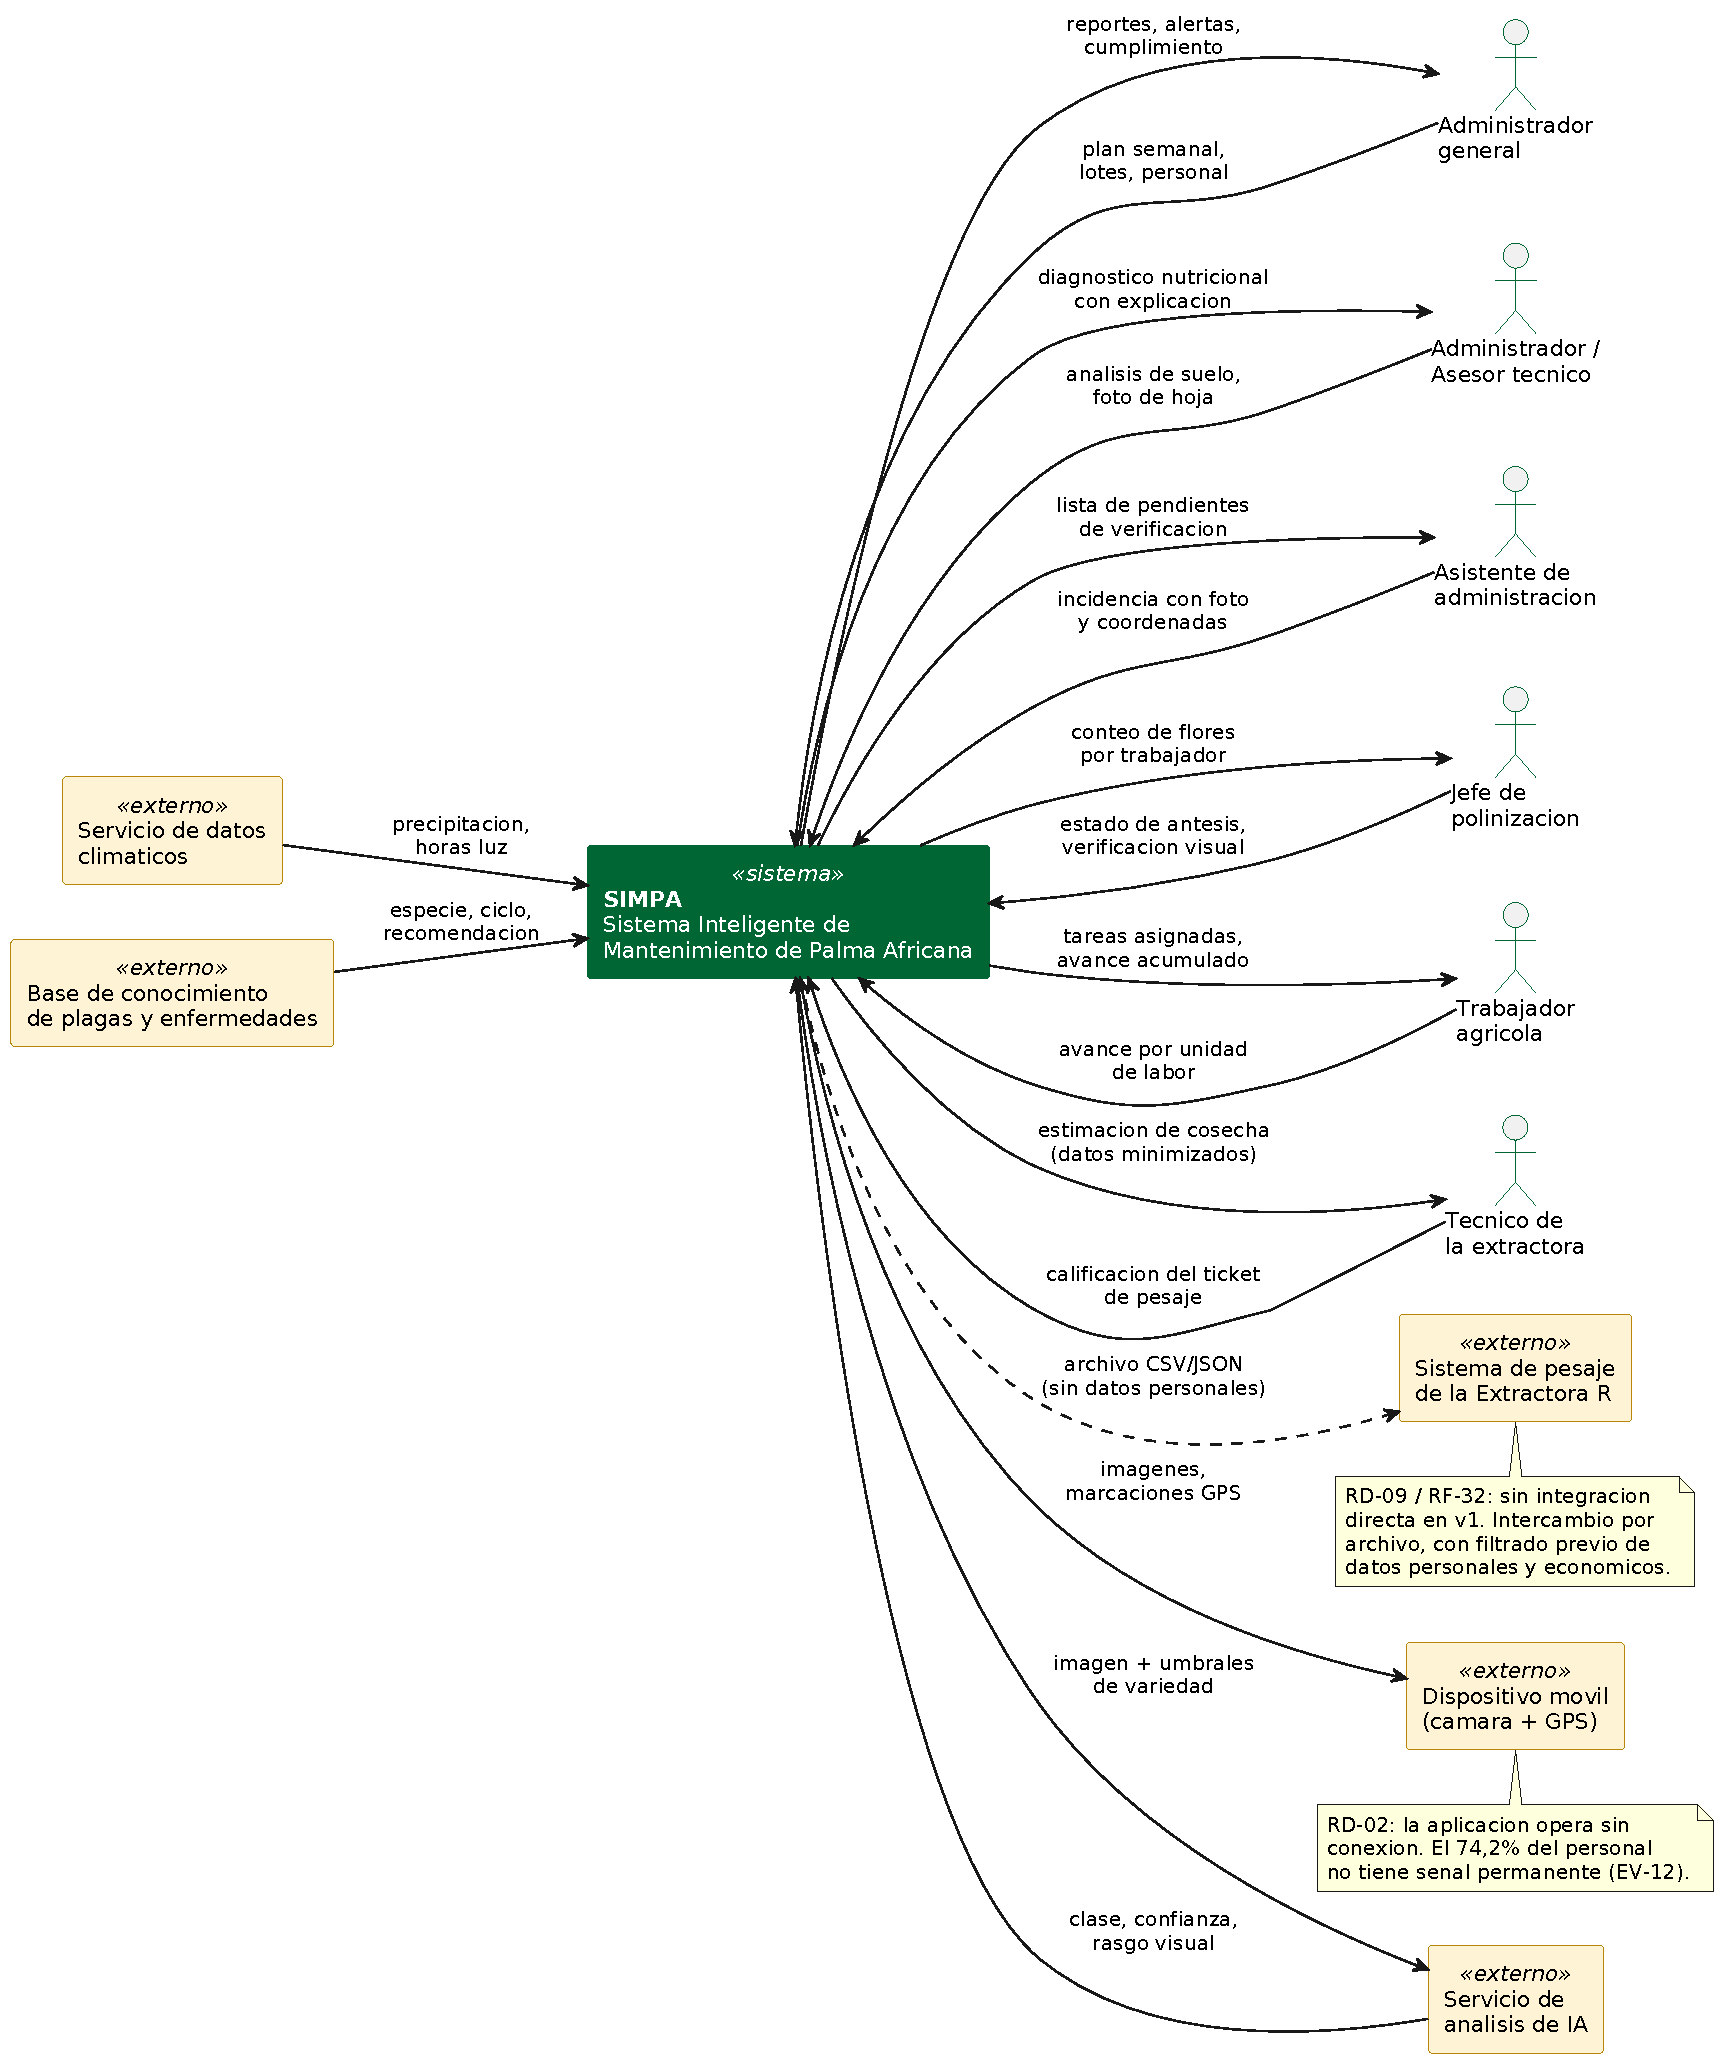
\includegraphics[width=1.0\textwidth]{img/contexto}
\caption{Diagrama de contexto del SIMPA (límite del sistema).}
\label{fig:contexto}
\end{figure}

\subsection{Funciones del producto}

Las funciones de alto nivel se agrupan en seis bloques: (i) gestión de la estructura productiva;
(ii) planificación y seguimiento de labores; (iii) registro operativo de campo; (iv) diagnóstico
asistido por IA; (v) control de calidad y relación con la extractora; y (vi) reportes y estimación
de producción. El detalle se especifica en la §3.2.

\subsection{Clases y características de los usuarios}

\begin{longtable}{|L{3.0cm}|L{5.4cm}|L{3.2cm}|L{2.8cm}|}
\hline
\rowcolor{grisclaro}\textbf{Perfil} & \textbf{Descripción} & \textbf{Competencia digital} & \textbf{Frecuencia de uso} \\
\hline
\endhead
Administrador general & Supervisión global del cultivo, decisiones de inversión y evaluación del personal (\id{EV-01}). & Media & Diaria \\ \hline
Administrador / Asesor técnico & Dirección técnica del cultivo; define nutrición, sanidad y manejo agrícola (\id{EV-02}). & Media & Semanal \\ \hline
Asistente de administración & Seguimiento de los trabajos de campo, verificación fotográfica de afectaciones, visitas dos veces por semana (\id{EV-07}). & \textbf{Alta} & Bisemanal \\ \hline
Jefe de polinización & Dirige la polinización asistida y controla su calidad (\id{EV-03}). & Media & Diaria \\ \hline
Trabajador agrícola & Ejecuta chapia, corona, polinización y cosecha; registra su avance (\id{EV-05}, \id{EV-06}). & \textbf{Baja} & Diaria \\ \hline
Técnico de la extractora & Califica la fruta recibida y asesora al productor sobre calidad (\id{EV-04}, \id{EV-08}). & Media-alta & Semanal \\ \hline
\caption{Clases de usuarios del SIMPA}
\end{longtable}

\noindent
La brecha de competencia digital entre el asistente de administración y el trabajador agrícola es
un hallazgo relevante para el diseño. El primero declaró estar familiarizado con este tipo de
tecnología y anticipó que \emph{``la dificultad podría presentarse principalmente con el personal de
campo que realiza labores manuales''} (\id{EV-07}). Esta observación sustenta la restricción
\id{RD-06} y el requisito de usabilidad \id{RNF-08}.

\subsection{Mapa de partes interesadas (matriz poder/interés)}

\begin{longtable}{|L{4.2cm}|C{1.8cm}|C{1.8cm}|L{3.4cm}|C{2.2cm}|}
\hline
\rowcolor{grisclaro}\textbf{Parte interesada} & \textbf{Poder} & \textbf{Interés} & \textbf{Estrategia} & \textbf{Evidencia} \\
\hline
\endhead
Propietario de la organización & Alto & Alto & Gestionar de cerca & \id{EV-02} \\ \hline
Administrador general & Alto & Alto & Gestionar de cerca & \id{EV-01} \\ \hline
Administrador / Asesor técnico & Alto & Alto & Gestionar de cerca & \id{EV-02} \\ \hline
Asistente de administración & Medio & Alto & Mantener informado & \id{EV-07} \\ \hline
Jefe de polinización & Medio & Alto & Mantener informado & \footnotesize \id{EV-03} \\ \hline
Planta extractora & \textbf{Alto} & Medio & \textbf{Mantener satisfecho} & \id{EV-04}, \id{EV-08} \\ \hline
Trabajadores agrícolas & Bajo & Alto & Mantener informados & \id{EV-05}, \id{EV-06} \\ \hline
Agrocalidad (ente regulador) & Alto & Bajo & Monitorear & \footnotesize \id{EV-04} \\ \hline
\caption{Mapa de partes interesadas con clasificación poder/interés}
\end{longtable}

\noindent
La incorporación de la planta extractora como parte interesada de \textbf{poder alto} es la
modificación más significativa respecto de la 1B. La extractora fija unilateralmente los criterios
de aceptación de la fruta, aplica castigos económicos sobre el lote y puede rechazar la carga
completa (\id{EV-04}). Su clasificación como parte de alto poder e interés medio refleja que, si
bien no es usuaria directa del SIMPA, sus criterios determinan el valor económico de la producción.

\subsection{Modelado organizacional i*}

\subsubsection{Diagrama de Dependencia Estratégica (SD)}

El modelo SD representa las dependencias entre actores del dominio, independientemente del sistema.
La Tabla~\ref{tab:sd} resume las dependencias identificadas a partir de la evidencia.

\begin{longtable}{|L{3.4cm}|L{3.4cm}|L{2.4cm}|L{4.4cm}|}
\hline
\rowcolor{grisclaro}\textbf{Actor dependiente} & \textbf{Actor depositario} & \textbf{Tipo} & \textbf{Elemento de dependencia} \\
\hline
\endhead
Propietario & Administrador general & Objetivo & Rendimiento de 40--45 t/ha/año (\id{EV-02}) \\ \hline
Administrador general & Jefe de campo & Recurso & Reporte diario de avance (\id{EV-07}) \\ \hline
Administrador general & Trabajador agrícola & Tarea & Ejecución de la labor presupuestada (\id{EV-11}) \\ \hline
Administrador general & Asistente de administración & Objetivo-blando & Oportunidad en la detección de afectaciones (\id{EV-07}) \\ \hline
Trabajador agrícola & Administrador general & Recurso & Asignación de lote y pago por avance (\id{EV-05}, \id{EV-06}) \\ \hline
Extractora & Cuadrilla de cosecha & Objetivo-blando & Fruta con desprendimiento suficiente (\id{EV-04}) \\ \hline
Extractora & Productor & Recurso & Estimación de tonelaje para planificar capacidad (\id{EV-04}) \\ \hline
Productor & Extractora & Recurso & Ticket de pesaje con calificación de calidad (\id{EV-04}) \\ \hline
Jefe de polinización & Polinizador & Tarea & Aplicación correcta del polinizante (\id{EV-03}) \\ \hline
\caption{Dependencias estratégicas (modelo i* SD)}
\label{tab:sd}
\end{longtable}

\noindent\textbf{Nota sobre la notación.} Los modelos i* se representan con la notación estándar de
Yu: objetivo (\emph{goal}) en rectángulo redondeado, objetivo-blando (\emph{softgoal}) en nube,
tarea (\emph{task}) en hexágono y recurso (\emph{resource}) en rectángulo. En el modelo SD, la
lectura de cada dependencia es \emph{depender} $\rightarrow$ \emph{dependum} $\rightarrow$
\emph{dependee}. Cada diagrama incorpora su leyenda.

\begin{figure}[!htbp]
\centering
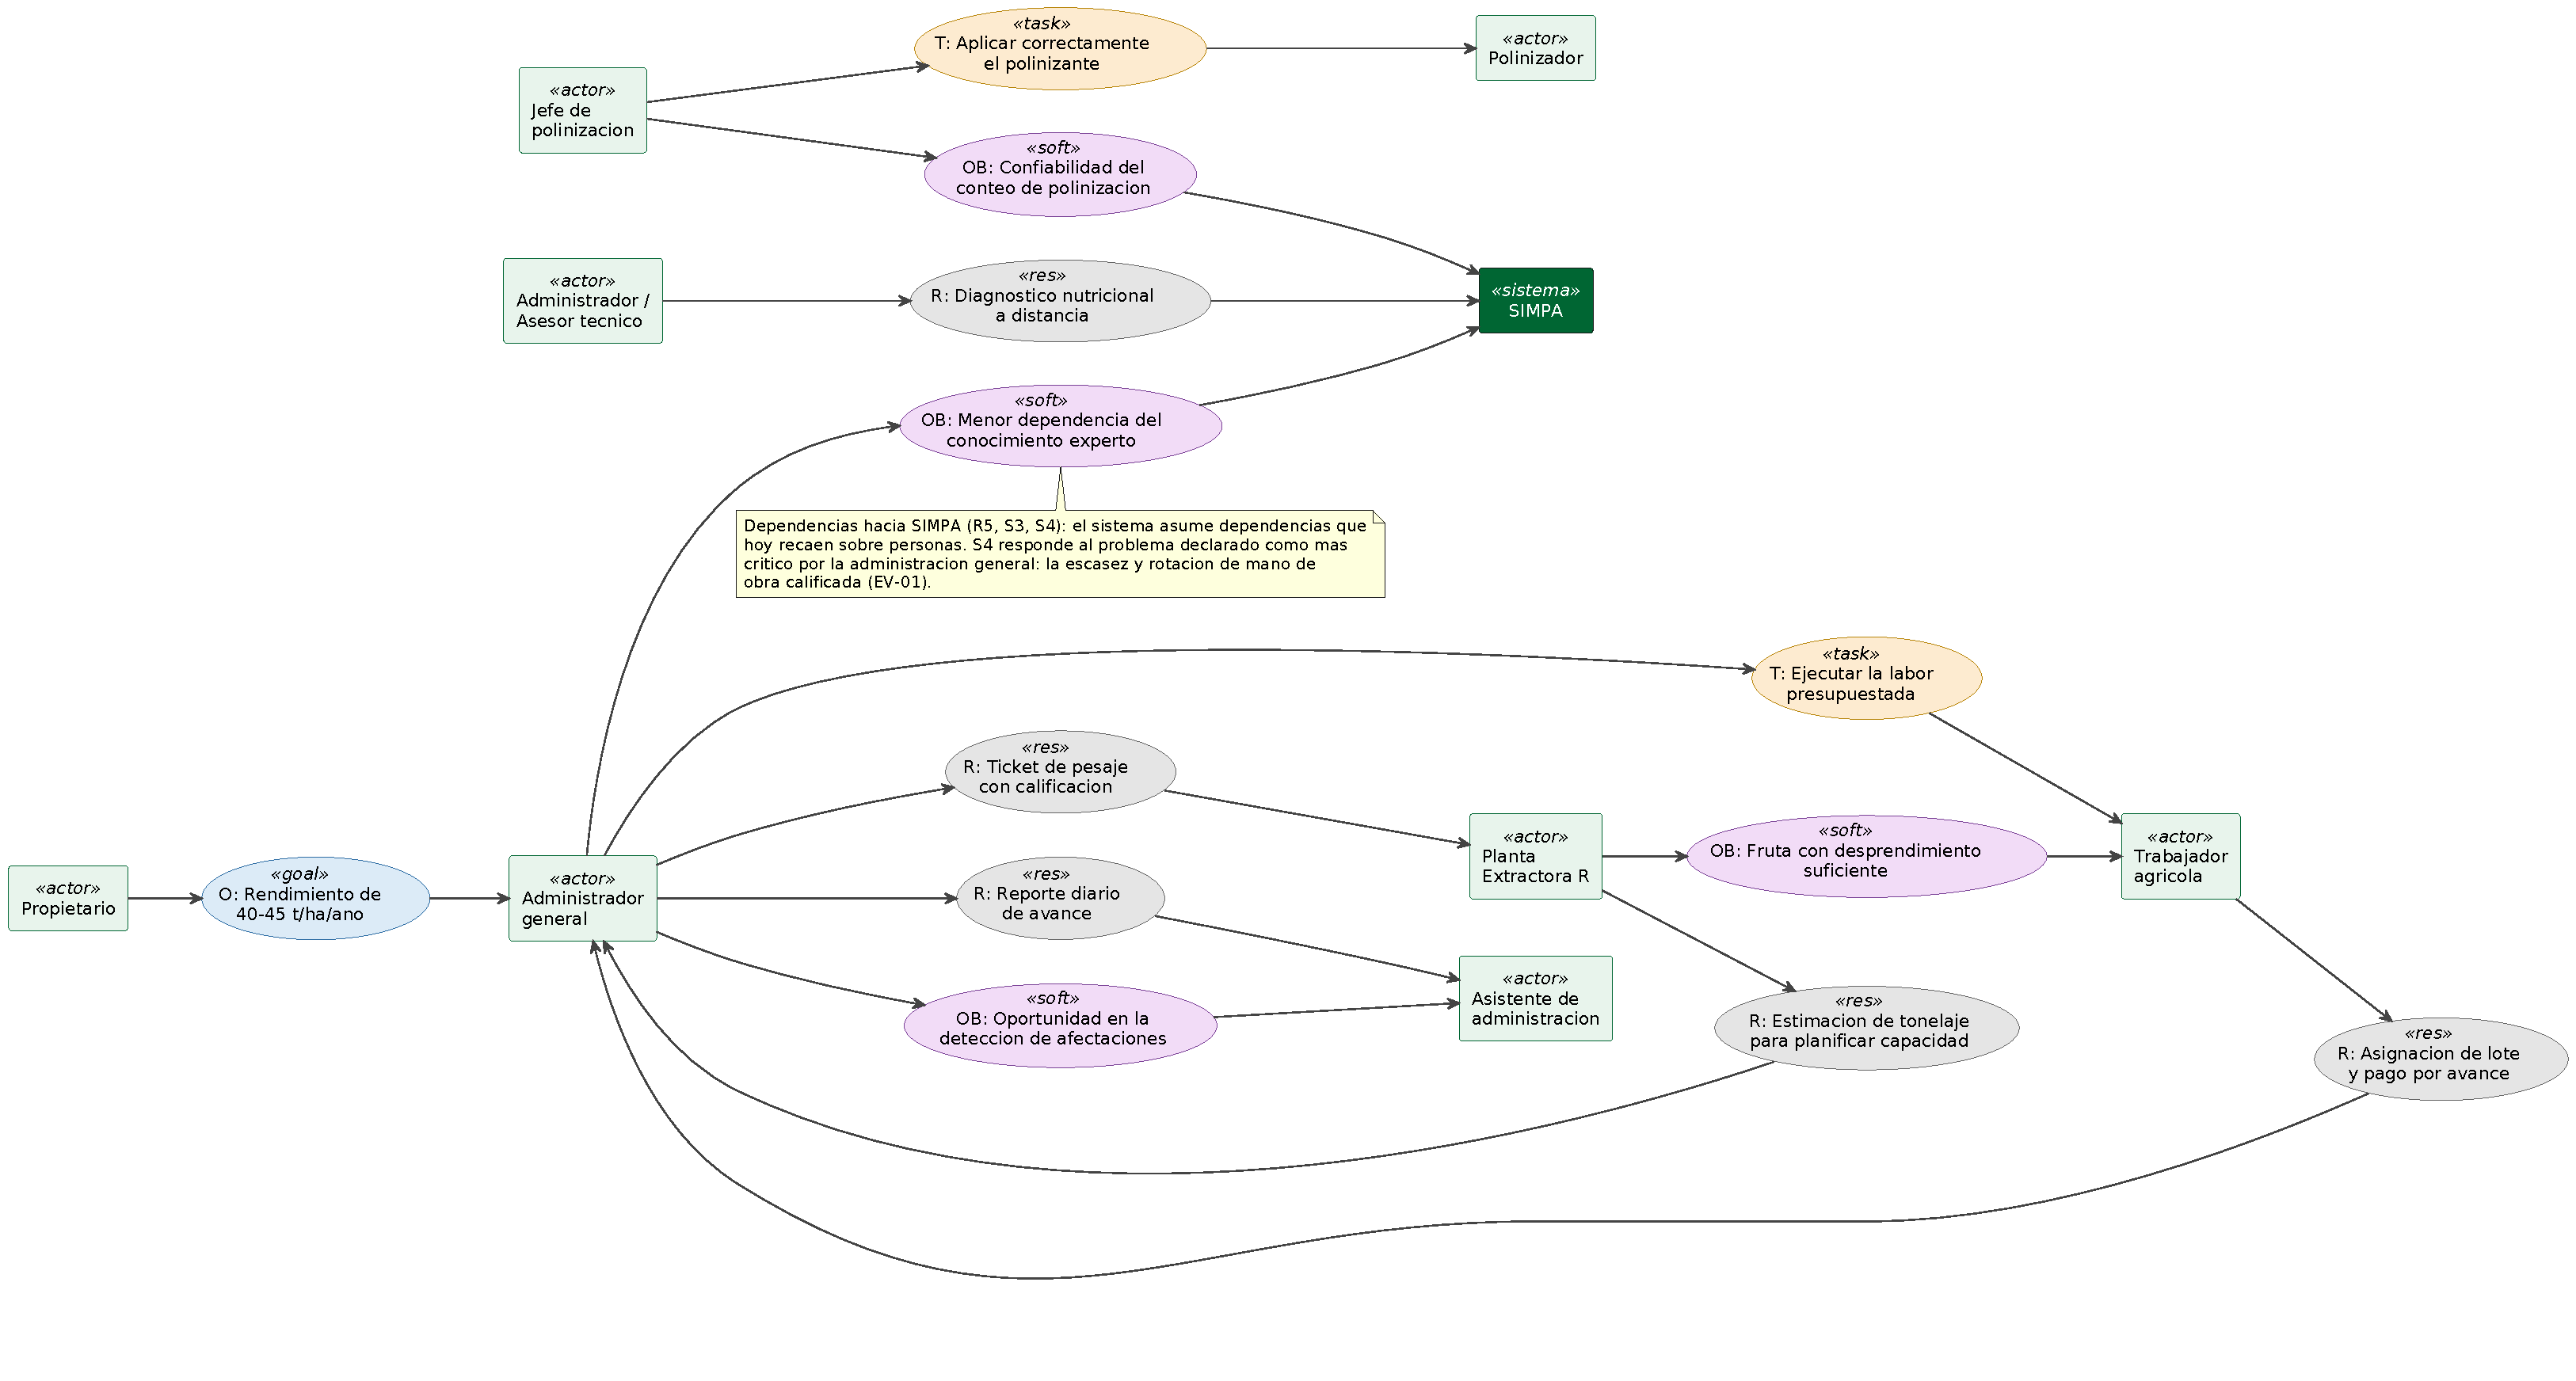
\includegraphics[width=1.0\textwidth]{img/istar_sd}
\caption{Diagrama de Dependencia Estratégica (i* SD) del dominio de Palmicultora M.}
\label{fig:sd}
\end{figure}

\subsubsection{Diagrama de Razón Estratégica (SR)}

El modelo SR profundiza en el actor \textbf{Administrador general}, cuyo objetivo raíz
\emph{``mantener el cultivo en estado productivo''} se descompone en cuatro tareas: supervisar
equipos de trabajo, controlar el estado sanitario, asegurar la humedad del suelo y verificar el
cumplimiento del presupuesto semanal. Sobre estas tareas actúan tres objetivos-blandos derivados de
la evidencia: \emph{oportunidad del diagnóstico} (\id{EV-01}: el recorrido completo toma una
semana), \emph{confiabilidad del conteo} (\id{EV-03}: el conteo manual afecta el rendimiento del
polinizador) y \emph{reducción de la dependencia del conocimiento experto} (\id{EV-01},
\id{EV-02}: la escasez de mano de obra calificada es el principal problema de gestión).

\begin{figure}[!htbp]
\centering
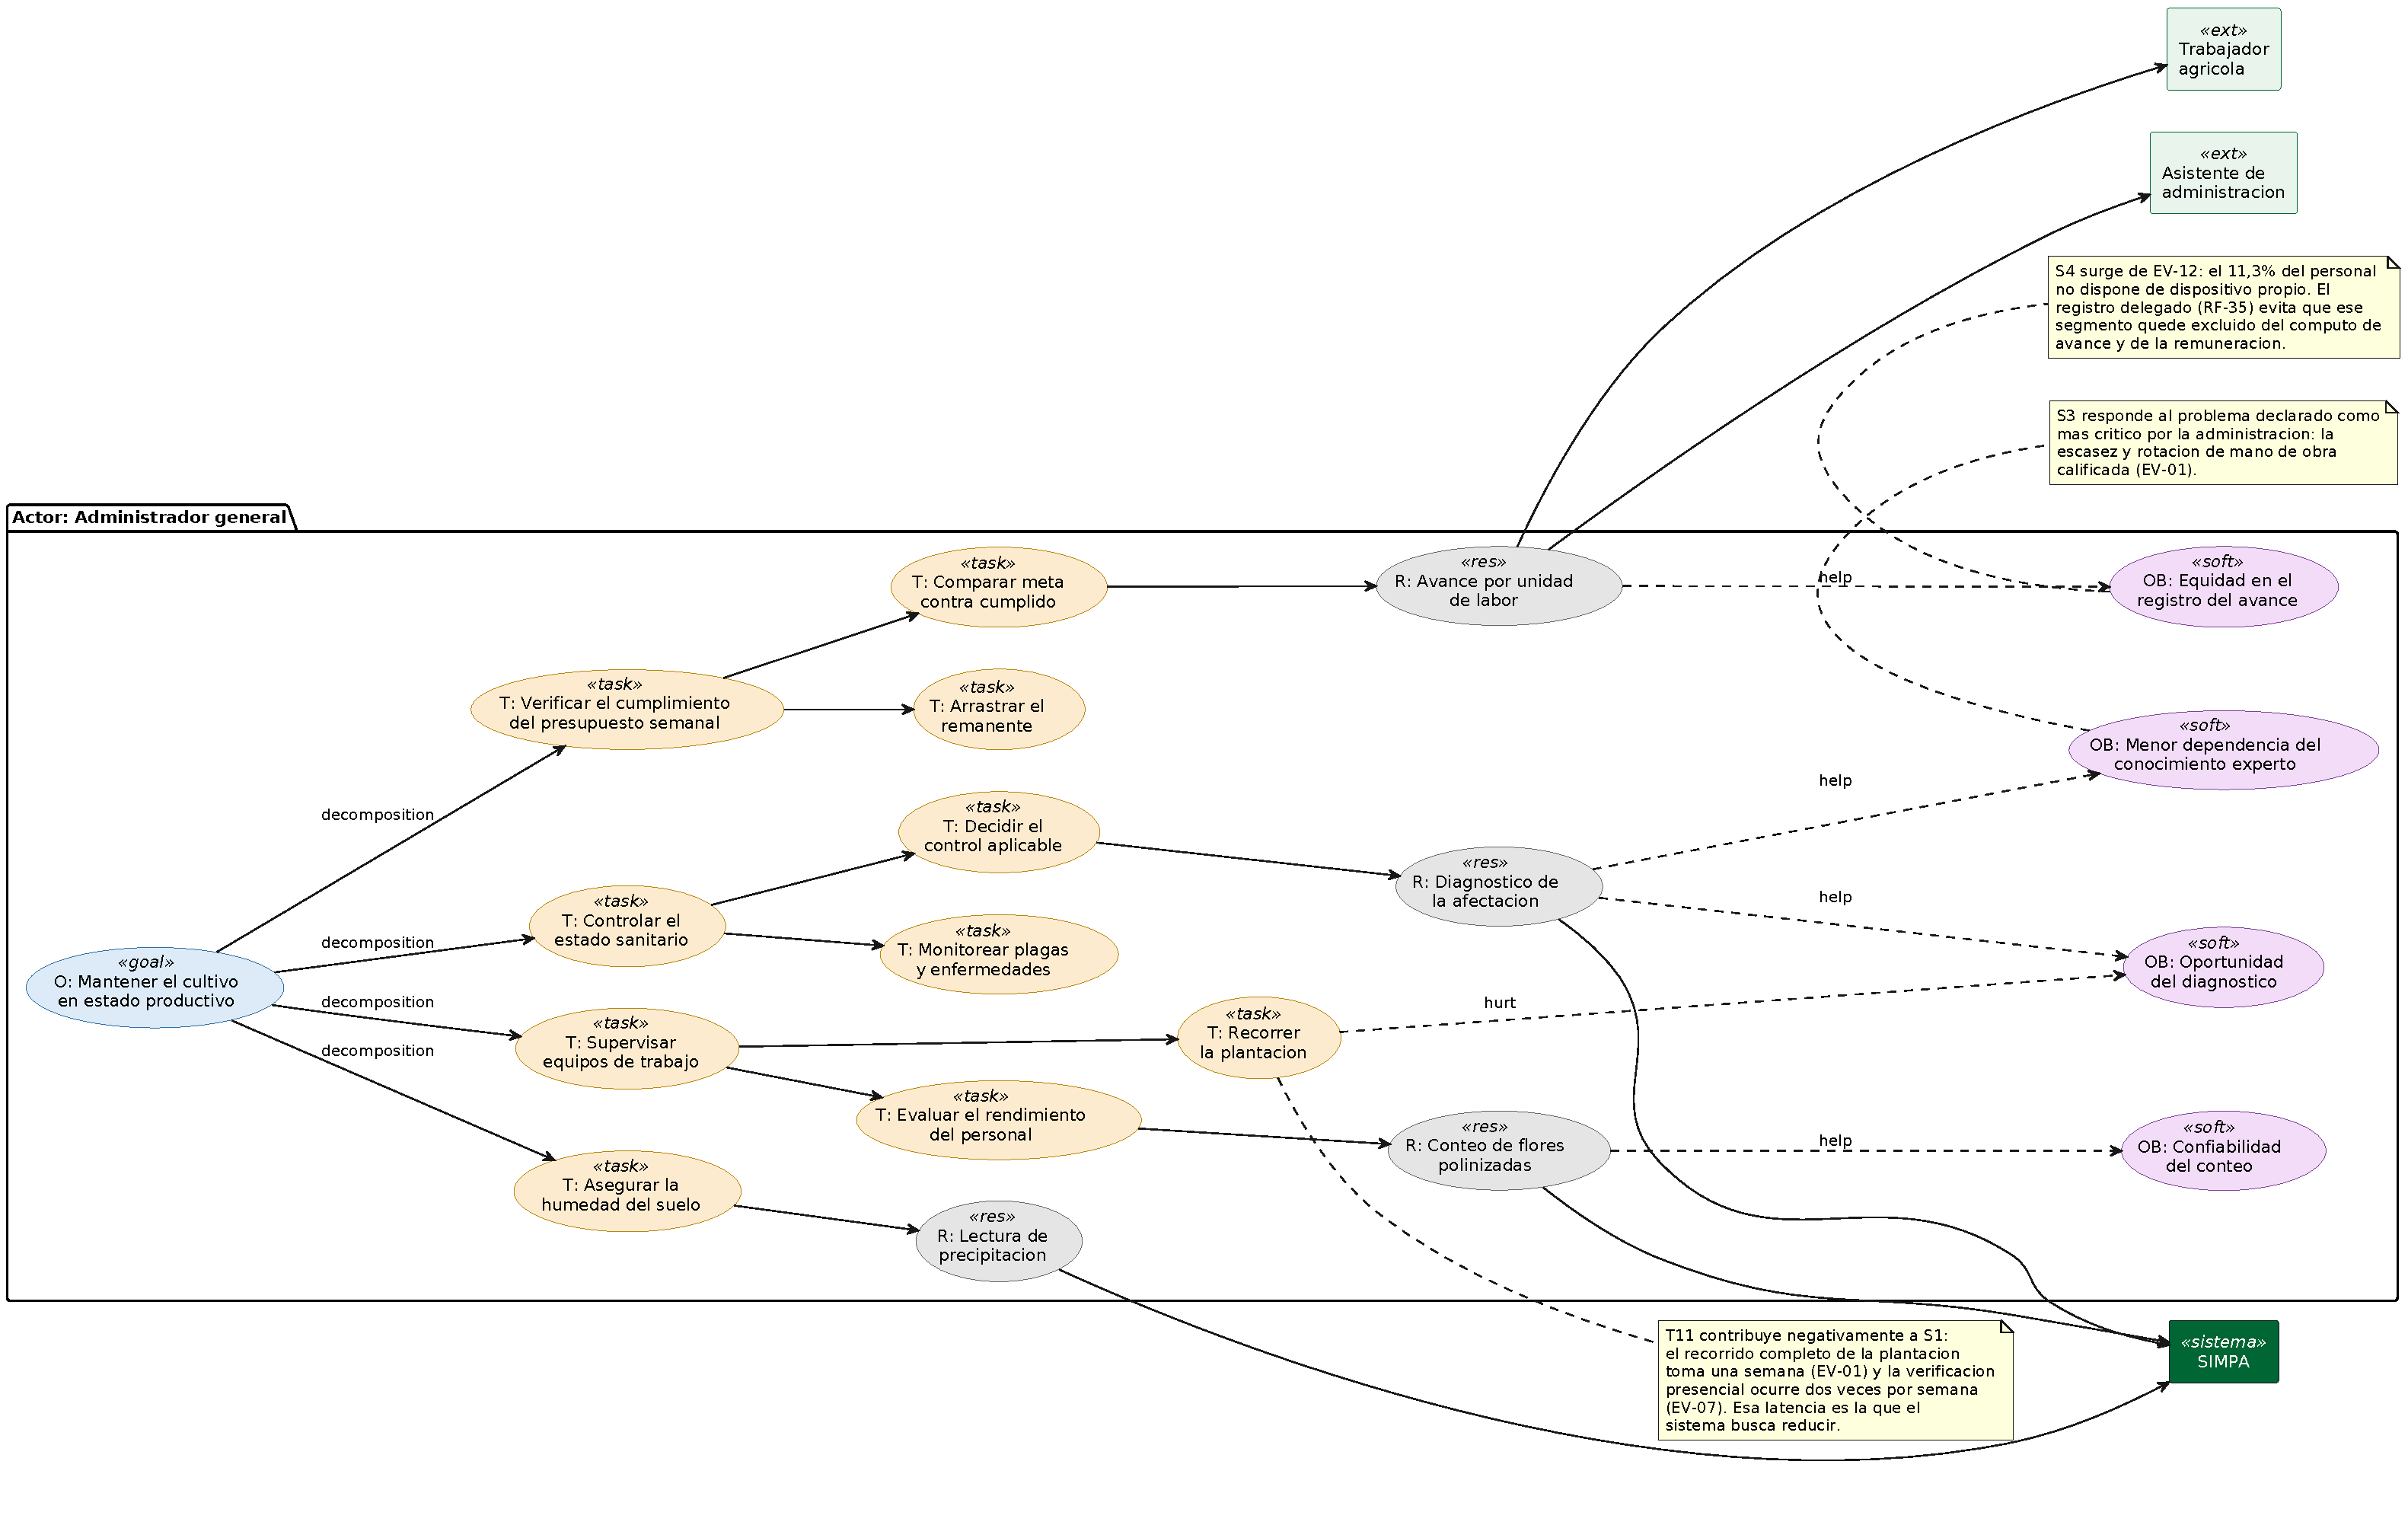
\includegraphics[width=1.0\textwidth]{img/istar_sr}
\caption{Diagrama de Razón Estratégica (i* SR) del actor Administrador general.}
\label{fig:sr}
\end{figure}

\subsection{Entorno operativo}

\textbf{Entorno físico.} Plantación de aproximadamente cien hectáreas dividida en seis lotes
(\id{EV-11}), con campamento y oficina administrativa. Condiciones de exposición solar directa,
humedad alta y jornadas que se extienden entre las 06:00 y las 18:00 según el clima (\id{EV-06}).

\textbf{Conectividad.} Existe internet satelital parcial; la conexión estable se limita al
campamento (\id{EV-07}). La aplicación ampliada del cuestionario ($n=62$, \id{EV-12}) precisa esta
condición: el 25{,}8\% de las personas respondientes declara disponer de señal siempre, el 51{,}6\%
solo a veces, el 21{,}0\% casi nunca y el 1{,}6\% nunca. Es decir, \textbf{el 74{,}2\% no cuenta con
conectividad permanente} en su zona de trabajo. Esta distribución --- y no la ausencia total de
señal --- es la que determina la arquitectura \emph{offline-first} del sistema: la aplicación debe
ser plenamente funcional sin conexión y sincronizar de forma oportunista.

\textbf{Plataforma.} Aplicación móvil Android para campo; panel web para administración; backend en
la nube con API REST y servicio de inferencia de IA.

\subsection{Suposiciones y dependencias}

\textbf{Suposiciones.} Las imágenes capturadas tienen calidad suficiente para el análisis; la
organización mantiene la práctica de planificación semanal documentada (\id{EV-11}); la
organización proveerá un mecanismo de registro asistido para el personal sin dispositivo propio.

\vspace{0.2cm}
\noindent\fbox{\parbox{0.97\textwidth}{%
\small\textbf{Suposición invalidada por la evidencia.} Las entregas anteriores asumían que la
totalidad del personal disponía de teléfono inteligente propio. La aplicación ampliada del
cuestionario ($n=62$, \id{EV-12}) refuta esa suposición: \textbf{el 11{,}3\% de las personas
respondientes declara no usar teléfono inteligente}. Esta constatación motiva la restricción
\id{RD-10} y el requisito \id{RF-35}, que habilitan el registro delegado para dicho segmento. De no
haberse corregido, el sistema habría excluido a aproximadamente una de cada nueve personas
destinatarias.}}

\textbf{Dependencias.} Disponibilidad del servicio de inferencia de IA; disponibilidad de datos
climáticos; vigencia del consentimiento informado de los trabajadores para el tratamiento de datos
de geolocalización.

\textbf{Riesgos.} Baja calidad de imagen en condiciones de contraluz; resistencia al uso de
tecnología por parte del personal de campo (\id{EV-07}); variabilidad del criterio de madurez entre
variedades, que exige parametrización (\id{EV-04}).


\subsection[Resultados del cuestionario aplicado (n=62)]{Resultados del cuestionario aplicado ($n=62$)}

El cuestionario se aplicó al personal de campo en dos rondas con \textbf{instrumento idéntico}, con
el fin de preservar la comparabilidad: una aplicación piloto de cuatro respondientes
(\id{EV-10}, 30/06/2026) y una aplicación ampliada de 62 respondientes (\id{EV-12}).

\textbf{Definición del perfil dominante.} La guía de la Entrega 3 exige $n \geq 30$ por perfil
dominante. En este estudio el perfil dominante es el de \textbf{trabajador agrícola de campo}, con
$n = 60$ (96{,}8\% de la muestra), estratificado en cuatro sub-perfiles según la labor principal.
Los estratos individuales no alcanzan por separado el umbral de 30; se declara explícitamente que el
análisis por estrato tiene carácter exploratorio y se reporta como limitación en la §7.

\begin{longtable}{|L{6.8cm}|C{2.0cm}|C{2.0cm}|L{3.6cm}|}
\hline
\rowcolor{grisclaro}\textbf{Variable} & \textbf{Valor} & \textbf{\%} & \textbf{Implicación} \\
\hline
\endhead
\multicolumn{4}{|l|}{\textbf{Perfil de la muestra}} \\ \hline
Polinización & 18 & 29{,}0 & Estrato mayor \\ \hline
Control fitosanitario & 18 & 29{,}0 & Estrato mayor \\ \hline
Labores de mantenimiento & 13 & 21{,}0 & --- \\ \hline
Riego & 11 & 17{,}7 & --- \\ \hline
Otra & 2 & 3{,}2 & Excluido del perfil dominante \\ \hline
\multicolumn{4}{|l|}{\textbf{Registro actual de la labor}} \\ \hline
En papel & 42 & 67{,}7 & Sustenta \id{RF-04}, \id{RF-28} \\ \hline
Lo anota la administración & 13 & 21{,}0 & Sustenta \id{RF-35} \\ \hline
No se registra & 6 & 9{,}7 & Pérdida de información \\ \hline
\multicolumn{4}{|l|}{\textbf{Mayor dificultad declarada} (selección múltiple)} \\ \hline
Detectar plagas o enfermedades a tiempo & 25 & 40{,}3 & Sustenta \id{RF-07}, \id{RF-12} \\ \hline
El clima & 21 & 33{,}9 & Sustenta \id{RF-17} \\ \hline
Llevar la cuenta de lo realizado & 13 & 21{,}0 & Sustenta \id{RF-28}, \id{RF-29} \\ \hline
Saber qué producto aplicar & 13 & 21{,}0 & Sustenta \id{RF-09} \\ \hline
Comunicación con la administración & 6 & 9{,}7 & Sustenta \id{RF-30} \\ \hline
\multicolumn{4}{|l|}{\textbf{Capacidad tecnológica}} \\ \hline
Usa teléfono inteligente & 55 & 88{,}7 & \textbf{11{,}3\% no lo usa}: \id{RD-10} \\ \hline
Comodidad con aplicaciones (media 1--5) & 3{,}14 & --- & Sustenta \id{RNF-08}, \id{RD-06} \\ \hline
Señal de internet permanente & 16 & 25{,}8 & \textbf{74{,}2\% sin señal permanente}: \id{RD-02} \\ \hline
\multicolumn{4}{|l|}{\textbf{Aceptación}} \\ \hline
No le preocupa el registro por GPS & 46 & 74{,}2 & \textbf{25{,}8\% con reservas}: \id{RL-03} \\ \hline
Usaría la aplicación & 53 & 85{,}5 & Adopción esperada \\ \hline
\caption{Resultados del cuestionario ampliado ($n=62$, \id{EV-12})}
\end{longtable}

\textbf{Utilidad percibida de las funciones propuestas.} Cada persona respondiente valoró cinco
funciones en escala de 1 a 5. El orden resultante confirma la priorización MoSCoW de la §5.

\begin{longtable}{|L{7.6cm}|C{1.8cm}|C{1.8cm}|C{2.6cm}|}
\hline
\rowcolor{grisclaro}\textbf{Función propuesta} & \textbf{Media} & \textbf{Mediana} & \textbf{Requisito} \\
\hline
\endhead
Recibir alertas ante un problema del cultivo & \textbf{4{,}31} & 5 & \id{RF-12} \\ \hline
Foto $\rightarrow$ detectar plaga o enfermedad & \textbf{4{,}27} & 5 & \id{RF-07} \\ \hline
Foto $\rightarrow$ detectar deficiencia nutricional & 4{,}10 & 4 & \id{RF-08} \\ \hline
Registrar labores en el teléfono & 3{,}95 & 4 & \id{RF-04}, \id{RF-28} \\ \hline
Conteo automático de flores por GPS & 3{,}94 & 4 & \id{RF-14} \\ \hline
\caption{Utilidad percibida de las funciones propuestas ($n=62$, escala 1--5)}
\end{longtable}

\noindent
Las dos funciones mejor valoradas ---alertas y detección de plagas por imagen--- coinciden con la
dificultad más declarada por el personal (detectar plagas a tiempo, 40{,}3\%) y con la necesidad
expresada de forma independiente por la administración general (\id{EV-01}) y la asesoría técnica
(\id{EV-02}). Esta convergencia entre tres fuentes distintas ---cuestionario, entrevista operativa y
entrevista directiva--- sustenta la clasificación \emph{Must} de \id{RF-07} y \id{RF-12}.

\textbf{Datos faltantes.} La pregunta sobre comodidad con aplicaciones registró 37 respuestas
válidas de 62 ($40{,}3\%$ de no respuesta). Este valor se reporta como limitación y no se emplea
para inferencia; la media de 3{,}14 se presenta únicamente como indicio descriptivo.

% =====================================================================
%  3. REQUISITOS ESPECIFICOS
% =====================================================================
\newpage
\section{Requisitos específicos}

Esta sección especifica 39 requisitos funcionales, 18 requisitos no funcionales cuantificados sobre
las nueve características de calidad de ISO/IEC 25010:2023 \cite{iso25010}, 9 restricciones de
diseño y el mapeo de requisitos legales a la LOPDP \cite{lopdp}.

\subsection{Interfaces externas}

\subsubsection{Interfaces de usuario}

Las pantallas principales se especifican mediante prototipos de alta fidelidad identificados
\id{MU-01} a \id{MU-08}, incrustados en el Apéndice F y disponibles como archivos PNG en
\id{03\_Modelado/Mockups/}. La Tabla~\ref{tab:mockups} traza cada prototipo con los requisitos que
soporta.

\begin{longtable}{|C{1.6cm}|L{5.6cm}|L{7.6cm}|}
\hline
\rowcolor{grisclaro}\textbf{ID} & \textbf{Pantalla} & \textbf{Requisitos soportados} \\
\hline
\endhead
\id{MU-01} & Inicio de sesión & \id{RF-01} \\ \hline
\id{MU-02} & Panel principal & \id{RF-12}, \id{RF-19}, \id{RF-26} \\ \hline
\id{MU-03} & Captura y análisis de imagen (IA) & \id{RF-07}, \id{RF-08}, \id{RF-09}, \id{RF-21} \\ \hline
\id{MU-04} & Registro de labor y polinización & \id{RF-04}, \id{RF-13}, \id{RF-14}, \id{RF-28} \\ \hline
\id{MU-05} & Detalle de lote & \id{RF-02}, \id{RF-05}, \id{RF-06}, \id{RF-11} \\ \hline
\id{MU-06} & Mapa de recorridos y polinización (GPS) & \id{RF-14}, \id{RF-15}, \id{RF-30} \\ \hline
\id{MU-07} & Reportes y estimación & \id{RF-18}, \id{RF-19}, \id{RF-32} \\ \hline
\id{MU-08} & Alertas & \id{RF-12}, \id{RF-22} \\ \hline
\caption{Trazabilidad entre prototipos de interfaz y requisitos funcionales}
\label{tab:mockups}
\end{longtable}

\subsubsection{Interfaces de hardware}

Cámara del dispositivo móvil (captura de imagen para los tres componentes de IA); receptor GPS
(conteo georreferenciado y registro de recorridos); dispositivo Android 9.0 o superior; servidor o
servicio en la nube para almacenamiento e inferencia.

\subsubsection{Interfaces de software}

API REST sobre HTTPS con carga útil JSON entre cliente móvil, panel web y backend; servicio de
inferencia de IA; servicio de autenticación con control de acceso basado en roles; base de datos
relacional; servicio de datos climáticos.

\subsubsection{Interfaces de comunicación}

Se incorpora en esta entrega la \textbf{interfaz de intercambio con la planta extractora}. La
evidencia \id{EV-04} documenta que la extractora opera un sistema interno propio que emite un ticket
de pesaje con peso bruto, tara, neto y calificación de calidad, y que lo remite al productor por
correo electrónico. El SIMPA no se integra directamente con ese sistema en la versión v1; el
intercambio se realiza mediante exportación de archivos en formato estructurado, conforme a
\id{RF-32} y a la restricción de minimización de datos \id{RD-09}.

\subsection{Requisitos funcionales}

Cada requisito se documenta con la plantilla de ocho atributos e incluye la referencia explícita al
identificador de evidencia que lo respalda, conforme a la §3.3 de la guía de la Entrega 3.

\subsubsection{Bloque I --- Gestión de la estructura productiva}

\RF{RF-01}{Autenticación y control de acceso por rol}
{El sistema debe permitir el inicio de sesión y restringir las funciones disponibles según el rol de la persona usuaria (administrador general, administrador/asesor técnico, asistente de administración, jefe de polinización, trabajador agrícola).}
{Administrador general · \id{EV-01}, \id{EV-07}, \id{EV-09}}
{\textbf{Entrada:} credenciales de acceso. \textbf{Salida:} sesión activa con menú correspondiente al rol, o mensaje de error.}
{\textbf{Pre:} la persona usuaria está registrada y activa. \textbf{Post:} accede únicamente a las funciones autorizadas para su rol.}
{Must}
{Una cuenta con rol \emph{trabajador agrícola} no puede acceder a ninguna función de administración; el acceso se concede exclusivamente con credenciales válidas.}

\RF{RF-02}{Gestión de plantaciones y lotes}
{El sistema debe permitir registrar, editar y consultar la plantación y sus lotes, con variedad sembrada, área en hectáreas, número de palmas y fecha de siembra.}
{Administrador general · \id{EV-01}, \id{EV-02}, \id{EV-11}}
{\textbf{Entrada:} datos identificativos y productivos del lote. \textbf{Salida:} lote almacenado y disponible en el listado.}
{\textbf{Pre:} persona usuaria con permiso de administración. \textbf{Post:} el lote queda disponible para asociar labores, diagnósticos y cosechas.}
{Must}
{Tras registrar un lote, este aparece en el listado y puede seleccionarse como destino de una labor, un diagnóstico y un registro de cosecha.}

\RF{RF-03}{Gestión de personal y equipos de trabajo}
{El sistema debe permitir registrar al personal y organizarlo por equipos funcionales: administración, polinización, control fitosanitario, riego y labores agrícolas.}
{Administrador general · \id{EV-01}, \id{EV-11}}
{\textbf{Entrada:} datos laborales de la persona trabajadora y equipo asignado. \textbf{Salida:} persona registrada y vinculada a un equipo.}
{\textbf{Pre:} persona usuaria con permiso de administración. \textbf{Post:} queda disponible para asignación de labores y cálculo de avance.}
{Must}
{Cada persona registrada queda asociada al menos a un equipo y aparece como asignable en el registro de labores.}

\RF{RF-10}{Gestión de variedades de palma}
{El sistema debe registrar la variedad sembrada por lote y emplearla para parametrizar los umbrales de diagnóstico y de madurez, así como las advertencias sobre polinizadores naturales.}
{Administrador / Asesor técnico · \id{EV-01}, \id{EV-02}, \id{EV-04}}
{\textbf{Entrada:} variedad asignada al lote y sus parámetros. \textbf{Salida:} umbrales aplicables a los módulos de diagnóstico y clasificación.}
{\textbf{Pre:} el lote existe. \textbf{Post:} los módulos de IA operan con los umbrales de la variedad correspondiente.}
{Must}
{Para un lote de variedad \emph{guineensis}, el umbral de madurez aplicado es de 3 frutos desprendidos; para un lote de variedad híbrida, de 5.}

\subsubsection{Bloque II --- Planificación y seguimiento de labores}

\RF{RF-26}{Planificación semanal de labores con presupuesto}
{El sistema debe permitir registrar el presupuesto semanal de labores por lote, expresado en la unidad de avance correspondiente, y contrastarlo con el avance efectivamente cumplido al cierre de la semana.}
{Administrador general · \id{EV-11}}
{\textbf{Entrada:} semana, lote, tipo de labor y meta en unidades. \textbf{Salida:} plan semanal y reporte comparativo presupuestado \emph{versus} cumplido.}
{\textbf{Pre:} los lotes y los tipos de labor están registrados. \textbf{Post:} el plan queda disponible para el seguimiento diario y el cierre semanal.}
{Must}
{Al cierre de una semana, el sistema muestra para cada labor planificada la meta, el avance cumplido y el porcentaje de cumplimiento.}

\RF{RF-27}{Arrastre de labor incompleta a la semana siguiente}
{Cuando una labor planificada no alcanza su meta al cierre de la semana, el sistema debe generar automáticamente el remanente como pendiente en el plan de la semana siguiente, conservando la referencia a la labor de origen.}
{Administrador general · \id{EV-11}}
{\textbf{Entrada:} cierre de la semana con avance inferior a la meta. \textbf{Salida:} labor pendiente creada en la semana siguiente con la cantidad remanente.}
{\textbf{Pre:} existe un plan semanal cerrado con cumplimiento parcial. \textbf{Post:} el remanente aparece en el plan siguiente marcado como continuación.}
{Should}
{Dada una meta de 1.123 coronas con 800 cumplidas, el sistema genera en la semana siguiente una labor pendiente de 323 coronas vinculada a la original.}

\RF{RF-34}{Registro de solicitud de insumos asociada al plan}
{El sistema debe permitir registrar los insumos requeridos para ejecutar el plan semanal y su estado de provisión.}
{Administrador general · \id{EV-11}}
{\textbf{Entrada:} insumo, cantidad y semana asociada. \textbf{Salida:} listado de requerimientos por semana con su estado.}
{\textbf{Pre:} existe un plan semanal. \textbf{Post:} el requerimiento queda asociado a la semana y consultable por la administración.}
{Could}
{Un insumo registrado como requerimiento de la semana aparece en el listado de la semana correspondiente con su estado de provisión.}

\RF{RF-36}{Catálogo codificado de labores con tarifa por unidad}
{El sistema debe mantener un catálogo de tipos de labor con su código identificador, su unidad de medida asociada (jornal, hora, avance o tonelada) y su tarifa vigente, de modo que la tarifa aplicable a un registro de avance se obtenga del catálogo y no se ingrese de forma manual en cada registro.}
{Administrador general · \id{EV-13}}
{\textbf{Entrada:} código de labor, unidad de medida, tarifa y fecha de vigencia. \textbf{Salida:} catálogo consultable y tarifa aplicable a cada registro de avance.}
{\textbf{Pre:} persona usuaria con permiso de administración. \textbf{Post:} los registros de avance posteriores emplean la tarifa vigente a su fecha.}
{Must}
{Registrada una labor de tipo corona con tarifa por unidad de avance, el cálculo del valor de un registro de 400 unidades corresponde al producto entre la cantidad y la tarifa vigente en la fecha del registro.}

\RF{RF-37}{Liquidación semanal de presupuesto contra ejecución}
{El sistema debe generar, al cierre de cada semana, una liquidación que contraste por grupo de labor la cantidad presupuestada, la cantidad ejecutada y el valor resultante, y que totalice el gasto presupuestado frente al gasto real.}
{Administrador general · \id{EV-13}, \id{EV-11}}
{\textbf{Entrada:} plan semanal y registros de avance del período. \textbf{Salida:} liquidación por grupo con totales y diferencia entre presupuestado y real.}
{\textbf{Pre:} existe un plan semanal y registros de avance asociados. \textbf{Post:} la liquidación queda disponible para aprobación.}
{Must}
{Para una semana con plan y avances registrados, el sistema presenta por cada grupo de labor la cantidad, la tarifa, el valor y el total, y calcula la diferencia entre el gasto presupuestado y el real.}

\RF{RF-38}{Registro de labor no presupuestada}
{El sistema debe permitir registrar labores ejecutadas que no figuraban en el plan de la semana, identificándolas de forma diferenciada para que no se confundan con el cumplimiento de las metas planificadas.}
{Administrador general · \id{EV-13}}
{\textbf{Entrada:} labor, cantidad, lote y motivo. \textbf{Salida:} registro marcado como no presupuestado, excluido del cálculo de cumplimiento del plan.}
{\textbf{Pre:} existe un plan semanal publicado. \textbf{Post:} la labor computa en el gasto real pero no en el cumplimiento de las metas.}
{Should}
{Una labor registrada como no presupuestada aparece en el grupo correspondiente de la liquidación y no altera el porcentaje de cumplimiento del plan.}

\RF{RF-39}{Aprobación de la liquidación semanal}
{El sistema debe requerir la aprobación explícita de la persona administradora para cerrar la liquidación de una semana, dejando constancia de quién aprobó y en qué fecha, tras lo cual los registros del período no admiten modificación sin trazabilidad.}
{Administrador general · \id{EV-13}}
{\textbf{Entrada:} liquidación semanal completa. \textbf{Salida:} liquidación cerrada con constancia de aprobación.}
{\textbf{Pre:} la liquidación de la semana está generada. \textbf{Post:} el período queda cerrado; toda modificación posterior genera entrada en bitácora.}
{Should}
{Aprobada una liquidación, el sistema registra la identidad de quien aprueba y la fecha, e impide modificar los registros del período sin dejar constancia.}


\RF{RF-35}{Registro delegado para personal sin dispositivo propio}
{El sistema debe permitir que una persona con rol de supervisión registre el avance de labor en nombre de una persona trabajadora que no dispone de teléfono inteligente, dejando constancia de quién efectuó el registro y en nombre de quién.}
{Jefe de campo / Asistente de administración · \id{EV-12}, \id{EV-05}}
{\textbf{Entrada:} identificación de la persona trabajadora, labor, cantidad y unidad. \textbf{Salida:} avance registrado a nombre de la persona trabajadora, con marca de registro delegado.}
{\textbf{Pre:} la persona registradora tiene rol de supervisión y la persona trabajadora está registrada. \textbf{Post:} el avance computa para la persona trabajadora y la bitácora conserva la identidad de quien lo registró.}
{Must}
{Un avance registrado de forma delegada aparece atribuido a la persona trabajadora en su consolidado, y la bitácora identifica a la persona supervisora que lo ingresó.}

\subsubsection{Bloque III --- Registro operativo de campo}

\RF{RF-04}{Registro de labores agrícolas}
{El sistema debe permitir registrar las labores ejecutadas por lote: chapia, corona, control químico de malezas, eliminación de flores andróginas, sanidad vegetal, poda, riego, polinización y cosecha.}
{Trabajador agrícola / Jefe de campo · \id{EV-01}, \id{EV-02}, \id{EV-05}, \id{EV-06}, \id{EV-11}}
{\textbf{Entrada:} tipo de labor, lote, fecha y persona responsable. \textbf{Salida:} labor registrada y asociada al lote, la fecha y la persona.}
{\textbf{Pre:} el lote y la persona trabajadora existen. \textbf{Post:} la labor queda en el historial del lote y computa para el avance.}
{Must}
{Una labor registrada queda vinculada a su lote, fecha y responsable, y es recuperable mediante consulta del historial del lote.}

\RF{RF-28}{Registro de avance por unidad de labor}
{El sistema debe registrar el avance diario de cada persona trabajadora en la unidad propia de cada labor: coronas, bancos, plantas, matas, jornales, racimos o toneladas, según corresponda al tipo de labor.}
{Trabajador agrícola · \id{EV-05}, \id{EV-06}, \id{EV-11}}
{\textbf{Entrada:} labor, cantidad ejecutada y unidad. \textbf{Salida:} avance diario acumulado por persona, lote y semana.}
{\textbf{Pre:} existe una labor asignada. \textbf{Post:} el avance queda registrado y disponible para el cálculo de cumplimiento y de remuneración por avance.}
{Must}
{Para una jornada de chapia, el sistema registra el número de matas ejecutadas y lo acumula al total semanal de la persona trabajadora.}

\RF{RF-29}{Consulta de avance acumulado y estimación de remuneración}
{El sistema debe permitir a la persona trabajadora consultar en su propio dispositivo el avance acumulado de la quincena y la estimación de remuneración correspondiente al trabajo por avance.}
{Trabajador agrícola · \id{EV-06}, \id{EV-07}}
{\textbf{Entrada:} identificación de la persona trabajadora y período. \textbf{Salida:} avance acumulado por labor y estimación de remuneración del período.}
{\textbf{Pre:} existen registros de avance en el período. \textbf{Post:} se muestra el consolidado sin posibilidad de edición por parte de la persona trabajadora.}
{Should}
{Una persona trabajadora consulta su avance quincenal y obtiene el desglose por labor y el valor estimado, coincidente con la suma de sus registros diarios.}

\RF{RF-05}{Registro de monitoreo fitosanitario}
{El sistema debe permitir registrar el monitoreo del estado fitosanitario por lote y marcar las incidencias detectadas.}
{Técnico fitosanitario · \id{EV-01}, \id{EV-02}, \id{EV-09}}
{\textbf{Entrada:} lote, observaciones y estado. \textbf{Salida:} registro de monitoreo y, si procede, alerta asociada.}
{\textbf{Pre:} persona usuaria autenticada. \textbf{Post:} el monitoreo queda disponible para consulta y reportes.}
{Must}
{El sistema almacena cada monitoreo con fecha y lote, y permite filtrar los lotes que presentan incidencia abierta.}

\RF{RF-30}{Reporte de incidencia desde campo con evidencia fotográfica y georreferencia}
{El sistema debe permitir reportar una afectación desde el campo adjuntando fotografía y coordenadas del punto exacto, de modo que la verificación posterior no dependa del recuerdo de la persona que reportó.}
{Asistente de administración · \id{EV-07}}
{\textbf{Entrada:} fotografía, lote, coordenadas y descripción. \textbf{Salida:} incidencia registrada y georreferenciada, visible en el mapa del lote.}
{\textbf{Pre:} persona usuaria autenticada con GPS disponible. \textbf{Post:} la incidencia queda pendiente de verificación con su ubicación exacta.}
{Must}
{Una incidencia reportada en campo es recuperable posteriormente con su fotografía y sus coordenadas, y su ubicación se muestra sobre el mapa del lote.}

\RF{RF-31}{Lista de verificación de pendientes por visita}
{El sistema debe mantener, para cada persona con rol de supervisión, una lista de actividades pendientes de verificación en su próxima visita a campo, alimentada por las incidencias reportadas.}
{Asistente de administración · \id{EV-07}}
{\textbf{Entrada:} incidencias reportadas y no verificadas. \textbf{Salida:} lista de pendientes ordenada por antigüedad y criticidad.}
{\textbf{Pre:} existen incidencias sin verificar. \textbf{Post:} la lista se actualiza al marcar cada pendiente como verificado.}
{Should}
{Al reportarse una incidencia, esta aparece en la lista de pendientes de la persona supervisora y desaparece al marcarse como verificada.}

\RF{RF-06}{Seguimiento de etapas del cultivo}
{El sistema debe registrar y dar seguimiento a la etapa del cultivo por lote: siembra, mantenimiento, polinización y cosecha.}
{Administrador general · \id{EV-01}}
{\textbf{Entrada:} etapa y fecha de transición por lote. \textbf{Salida:} línea de tiempo de etapas del lote.}
{\textbf{Pre:} el lote existe. \textbf{Post:} la etapa actual queda actualizada.}
{Should}
{Cada lote muestra su etapa actual y el historial completo de transiciones con sus fechas.}

\RF{RF-11}{Registro de análisis de suelo y foliar}
{El sistema debe registrar los resultados de los análisis de suelo y foliar por lote, incluyendo nitrógeno, fósforo, potasio y elementos menores, para guiar la fertilización.}
{Administrador / Asesor técnico · \id{EV-02}, \id{EV-04}}
{\textbf{Entrada:} valores del análisis por lote y fecha. \textbf{Salida:} registro histórico y comparativo por lote.}
{\textbf{Pre:} el lote existe. \textbf{Post:} el análisis queda asociado al lote y consultable por fecha.}
{Should}
{Tras registrar un análisis, sus valores quedan asociados al lote y pueden compararse con los análisis previos del mismo lote.}

\RF{RF-17}{Registro y consulta de datos climáticos}
{El sistema debe registrar y permitir consultar los datos climáticos del cultivo: milímetros de lluvia medidos con pluviómetro y datos de estaciones meteorológicas.}
{Administrador general / Asesor técnico · \id{EV-01}, \id{EV-02}, \id{EV-03}}
{\textbf{Entrada:} lectura de precipitación y fecha. \textbf{Salida:} histórico climático y consulta de lluvia acumulada por período.}
{\textbf{Pre:} persona usuaria autenticada. \textbf{Post:} la lectura queda incorporada al registro climático del cultivo.}
{Should}
{El sistema permite consultar la precipitación acumulada en un rango de fechas definido por la persona usuaria.}

\subsubsection{Bloque IV --- Polinización asistida}

\RF{RF-13}{Registro del proceso de polinización}
{El sistema debe registrar la polinización por lote, incluyendo el estado de la antesis (coloración amarilla o negra) y la verificación visual de la aplicación del polinizante.}
{Jefe de polinización / Polinizador · \id{EV-03}}
{\textbf{Entrada:} lote, estado de antesis y verificación visual. \textbf{Salida:} registro de polinización asociado al lote, fecha y persona.}
{\textbf{Pre:} el lote se encuentra en etapa de polinización. \textbf{Post:} el registro queda disponible para el control de calidad de la labor.}
{Must}
{El sistema permite registrar la polinización indicando el estado de antesis y consultar los lotes polinizados en una fecha dada.}

\RF{RF-14}{Conteo georreferenciado de flores polinizadas}
{El sistema debe calcular automáticamente, a partir de las marcaciones georreferenciadas registradas durante la jornada, el número de flores polinizadas por cada persona trabajadora, sin requerir el ingreso manual planta por planta.}
{Polinizador · \id{EV-03}}
{\textbf{Entrada:} marcaciones georreferenciadas de la jornada. \textbf{Salida:} total diario de flores polinizadas por persona y lote.}
{\textbf{Pre:} sesión iniciada con rastreo GPS activo. \textbf{Post:} el conteo queda registrado sin intervención manual por planta.}
{Must}
{Al cierre de la jornada, el sistema calcula el total de flores polinizadas por persona a partir de las marcaciones GPS, sin registro manual individual.}

\RF{RF-15}{Registro y visualización de recorridos del personal}
{El sistema debe registrar y mostrar los recorridos georreferenciados del personal en campo, con el fin de verificar la cobertura efectiva de las labores asignadas.}
{Administrador general · \id{EV-01}, \id{EV-02}, \id{EV-03}}
{\textbf{Entrada:} secuencia de ubicaciones durante la jornada. \textbf{Salida:} recorrido representado sobre el mapa del lote, por persona y fecha.}
{\textbf{Pre:} la persona trabajadora ha otorgado consentimiento para el tratamiento de datos de geolocalización (véase \id{RL-03}). \textbf{Post:} el recorrido queda disponible para supervisión.}
{Should}
{La administración puede visualizar el recorrido de una persona trabajadora en una fecha determinada, siempre que exista consentimiento vigente.}

\RF{RF-16}{Evaluación de desempeño del personal}
{El sistema debe calcular indicadores de desempeño por persona trabajadora a partir del avance registrado, la cobertura de los recorridos y la calidad resultante de la fruta cosechada en los lotes bajo su responsabilidad.}
{Administrador general · \id{EV-01}, \id{EV-02}, \id{EV-03}}
{\textbf{Entrada:} registros de avance, recorridos y calificaciones de calidad del período. \textbf{Salida:} indicador de desempeño por persona y período.}
{\textbf{Pre:} existen registros suficientes en el período. \textbf{Post:} el indicador queda disponible para consulta de la administración.}
{Should}
{Para un período dado, el sistema calcula un indicador de desempeño por persona a partir de sus registros, sin intervención manual.}

\subsubsection{Bloque V --- Diagnóstico asistido por inteligencia artificial}

\noindent\textbf{Viabilidad técnica de los componentes de IA.} Los tres requisitos de análisis de
imagen de este bloque no son especulativos: la literatura reciente documenta implementaciones
equivalentes en el mismo cultivo. La clasificación de madurez de racimos de palma aceitera
\emph{sobre dispositivos móviles} mediante aprendizaje profundo ha sido reportada por Suharjito
\emph{et al.} \cite{suharjito2021}, y la revisión de Goh \emph{et al.} \cite{goh2025} sistematiza
los métodos disponibles y sus tasas de acierto. Existen además conjuntos de datos públicos de
racimos capturados en exteriores \cite{omar2024} y aproximaciones basadas en segmentación y
características texturales \cite{rosbi2024} que evitan la dependencia del color, consistente con la
restricción \id{RD-07}. Rizzo \emph{et al.} \cite{rizzo2023} ofrecen el panorama general de la
clasificación de madurez de frutos, y Kipli \emph{et al.} \cite{kipli2023} documentan aplicaciones
de detección y conteo de palmas. Zaki \emph{et al.} \cite{zaki2025} sitúan estas tecnologías dentro
de la transformación digital del sector palmicultor. Estas fuentes sustentan los valores objetivo
fijados en \id{RNF-01} y \id{RNF-02}.

\vspace{0.3cm}
\RF{RF-07}{Detección de plagas y enfermedades por análisis de imagen}
{El sistema debe analizar una fotografía de la palma e identificar la presencia de plagas o enfermedades, indicando el tipo probable de afectación.}
{Técnico fitosanitario / Trabajador agrícola · \id{EV-01}, \id{EV-02}, \id{EV-08}}
{\textbf{Entrada:} fotografía de la palma o de la hoja. \textbf{Salida:} clasificación de la afectación con nivel de confianza y explicación asociada (véase \id{RNF-16}).}
{\textbf{Pre:} la imagen cumple los requisitos mínimos de calidad. \textbf{Post:} el diagnóstico queda asociado al lote y a la fecha.}
{Must}
{Ante un conjunto de imágenes de prueba con afectación previamente conocida, el sistema devuelve la clasificación correspondiente y la registra con su lote y fecha.}

\RF{RF-08}{Diagnóstico de deficiencias nutricionales por análisis de imagen}
{El sistema debe analizar la fotografía de una hoja y estimar la deficiencia nutricional presente, sugiriendo la corrección correspondiente.}
{Administrador / Asesor técnico · \id{EV-02}, \id{EV-04}}
{\textbf{Entrada:} fotografía de la hoja. \textbf{Salida:} deficiencia estimada, recomendación de fertilización y explicación asociada.}
{\textbf{Pre:} imagen válida y lote con variedad asignada. \textbf{Post:} el diagnóstico nutricional queda registrado en el historial del lote.}
{Must}
{Ante una hoja con deficiencia previamente conocida, el sistema indica la deficiencia, propone una corrección y almacena el registro.}

\RF{RF-09}{Ficha técnica de plaga con recomendación de control}
{El sistema debe presentar, para cada plaga detectada, su especie o familia, su ciclo de evolución y la acción de control recomendada según la etapa del insecto.}
{Técnico fitosanitario · \id{EV-01}, \id{EV-02}}
{\textbf{Entrada:} plaga identificada por \id{RF-07}. \textbf{Salida:} ficha con especie, ciclo y acción recomendada diferenciada por etapa.}
{\textbf{Pre:} existe un diagnóstico de plaga. \textbf{Post:} la recomendación queda disponible y registrada junto al diagnóstico.}
{Should}
{Para una plaga detectada en estado adulto, el sistema recomienda trampeo; para la misma plaga en estado larval, recomienda aplicación de insecticida.}

\RF{RF-21}{Clasificación de madurez del racimo por desprendimiento}
{El sistema debe estimar el estado de madurez de un racimo a partir de una fotografía de su parte basal, empleando el conteo de frutos desprendidos como criterio y aplicando el umbral correspondiente a la variedad del lote. El sistema no debe emplear el color del fruto como criterio de clasificación.}
{Técnico de la extractora / Cosechador · \id{EV-04}, \id{EV-08}}
{\textbf{Entrada:} fotografía de la parte basal del racimo y variedad del lote. \textbf{Salida:} estado estimado (verde, maduro, sobremaduro) con nivel de confianza y explicación.}
{\textbf{Pre:} el lote tiene variedad asignada (\id{RF-10}). \textbf{Post:} la estimación queda asociada al racimo, el lote y la fecha.}
{Must}
{Para un lote de variedad híbrida, un racimo con menos de 5 frutos desprendidos se clasifica como verde; con 5 o más, como maduro. Para variedad \emph{guineensis} el umbral aplicado es de 3.}

\RF{RF-12}{Generación de alertas tempranas}
{El sistema debe generar alertas ante la detección de plagas, enfermedades, deficiencias nutricionales o condiciones anómalas, dirigidas al rol responsable de su atención.}
{Técnico / Administrador general · \id{EV-01}, \id{EV-02}}
{\textbf{Entrada:} diagnóstico o incidencia registrada. \textbf{Salida:} alerta con lote, tipo, criticidad y fecha, visible para el rol correspondiente.}
{\textbf{Pre:} existe una incidencia o diagnóstico positivo. \textbf{Post:} la alerta queda registrada con estado abierto hasta su atención.}
{Must}
{Al registrarse un diagnóstico positivo, el sistema genera una alerta asociada al lote, visible para la administración, con estado y fecha.}

\subsubsection{Bloque VI --- Calidad de la fruta y relación con la extractora}

\RF{RF-22}{Estimación y alerta preventiva de porcentaje de fruta verde}
{El sistema debe estimar, antes del despacho de un lote cosechado, el porcentaje de racimos clasificados como verdes, y emitir una alerta cuando dicho porcentaje se aproxime al umbral a partir del cual la planta extractora aplica penalización.}
{Administrador general / Técnico de la extractora · \id{EV-04}, \id{EV-08}}
{\textbf{Entrada:} clasificaciones de madurez del lote cosechado (\id{RF-21}). \textbf{Salida:} porcentaje estimado de fruta verde y alerta si supera el umbral configurado.}
{\textbf{Pre:} existen racimos clasificados en el lote. \textbf{Post:} la alerta queda registrada antes del despacho.}
{Must}
{Configurado un umbral del 3\%, un lote cuya estimación de fruta verde alcance o supere ese valor genera una alerta previa al despacho.}

\RF{RF-23}{Registro de la calificación de calidad emitida por la extractora}
{El sistema debe permitir registrar los datos del ticket de pesaje emitido por la planta extractora: peso bruto, tara, peso neto y calificación de calidad (tamaño del fruto, fruta verde, sobremadura, malformada y pedúnculo largo).}
{Administrador general · \id{EV-04}}
{\textbf{Entrada:} datos del ticket de pesaje. \textbf{Salida:} registro de entrega asociado al lote y a la fecha, con su calificación.}
{\textbf{Pre:} existe un despacho registrado. \textbf{Post:} la calificación queda asociada al lote de origen y disponible para análisis histórico.}
{Should}
{Registrado un ticket, sus valores quedan asociados al lote de origen y son consultables en el histórico de entregas.}

\RF{RF-24}{Trazabilidad de la calificación hasta la cuadrilla responsable}
{El sistema debe permitir rastrear una calificación desfavorable de la extractora hasta el lote de origen, la fecha de corte y la cuadrilla de cosecha responsable, con el fin de distinguir si el problema proviene de la cosecha o del manejo del cultivo.}
{Técnico de la extractora / Administrador general · \id{EV-04}, \id{EV-08}}
{\textbf{Entrada:} identificación del despacho calificado. \textbf{Salida:} lote, fecha de corte, cuadrilla y labores asociadas al período.}
{\textbf{Pre:} el despacho tiene calificación registrada y el lote tiene labores registradas. \textbf{Post:} se muestra la cadena completa de trazabilidad.}
{Should}
{Dado un despacho con penalización por fruta verde, el sistema identifica el lote, la fecha de corte y la cuadrilla que ejecutó la cosecha.}

\RF{RF-25}{Control de la ventana entre corte y entrega}
{El sistema debe registrar la fecha y hora de corte de cada lote cosechado y calcular el tiempo transcurrido hasta la entrega en la planta extractora, emitiendo una advertencia cuando dicho intervalo supere el valor recomendado para la variedad.}
{Técnico de la extractora · \id{EV-04}}
{\textbf{Entrada:} marca temporal de corte y de entrega. \textbf{Salida:} intervalo calculado y advertencia si excede el umbral configurado.}
{\textbf{Pre:} existe un registro de cosecha con marca temporal. \textbf{Post:} el intervalo queda registrado junto al despacho.}
{Should}
{Configurado un umbral de 24 horas, un despacho entregado 30 horas después del corte genera la advertencia correspondiente.}

\RF{RF-33}{Registro de la guía de remisión del despacho}
{El sistema debe permitir registrar el número y la fecha de la guía de remisión asociada a cada despacho de fruta, y advertir cuando un despacho se registre sin ella.}
{Técnico de la extractora · \id{EV-04}}
{\textbf{Entrada:} número y fecha de la guía de remisión. \textbf{Salida:} despacho con guía asociada, o advertencia de ausencia.}
{\textbf{Pre:} existe un despacho registrado. \textbf{Post:} la guía queda vinculada al despacho.}
{Could}
{Un despacho registrado sin número de guía de remisión genera una advertencia visible para la administración antes de su cierre.}

\subsubsection{Bloque VII --- Reportes, estimación e histórico}

\RF{RF-18}{Estimación de producción y rendimiento}
{El sistema debe estimar la producción futura a partir del censo de flores, el número de racimos en desarrollo y el rendimiento propio de la variedad sembrada.}
{Administrador general / Asesor técnico · \id{EV-01}, \id{EV-02}}
{\textbf{Entrada:} censo de flores, conteo de racimos y variedad. \textbf{Salida:} estimación de producción por lote y período.}
{\textbf{Pre:} existe al menos un censo registrado. \textbf{Post:} la estimación queda disponible para la planificación.}
{Must}
{A partir de un censo y de la variedad del lote, el sistema calcula una estimación de producción consultable por lote y período.}

\RF{RF-32}{Compartición de la estimación de cosecha con la planta extractora}
{El sistema debe permitir exportar la estimación de cosecha del período hacia la planta extractora, limitando la información compartida al conteo de racimos y al peso promedio estimado, con exclusión de cualquier dato personal o económico.}
{Técnico de la extractora · \id{EV-04}}
{\textbf{Entrada:} período y lotes seleccionados. \textbf{Salida:} archivo estructurado con conteo de racimos y peso promedio estimado.}
{\textbf{Pre:} existe una estimación calculada. \textbf{Post:} el archivo queda disponible para su envío, sin contener datos personales.}
{Should}
{El archivo exportado contiene exclusivamente conteo de racimos y peso promedio por período, y no incluye ningún campo de identificación personal ni información económica.}

\RF{RF-19}{Generación de reportes}
{El sistema debe generar reportes diarios, consolidados semanales y estadísticas anuales sobre el estado del cultivo, las labores ejecutadas, el personal y la producción.}
{Administrador general · \id{EV-01}, \id{EV-02}, \id{EV-11}}
{\textbf{Entrada:} tipo de reporte y período. \textbf{Salida:} reporte consolidado, exportable a PDF y a hoja de cálculo.}
{\textbf{Pre:} existen registros en el período seleccionado. \textbf{Post:} el reporte queda disponible para consulta o exportación.}
{Must}
{El sistema genera el consolidado semanal de labores y producción del período seleccionado y permite exportarlo.}

\RF{RF-20}{Historial de actividades, diagnósticos y eventos}
{El sistema debe mantener un historial consultable y filtrable de todas las actividades, diagnósticos, alertas y entregas asociadas a cada lote.}
{Administrador general / Técnico · \id{EV-01}}
{\textbf{Entrada:} filtros por lote, fecha y tipo de evento. \textbf{Salida:} historial cronológico filtrado.}
{\textbf{Pre:} existen registros previos. \textbf{Post:} se muestra el historial conforme a los filtros aplicados.}
{Should}
{La persona usuaria puede recuperar, filtrando por lote y rango de fechas, el historial completo de actividades y diagnósticos registrados.}

\subsection{Requisitos no funcionales (ISO/IEC 25010:2023)}

Los dieciocho requisitos no funcionales se organizan según las nueve características de calidad del
producto de ISO/IEC 25010:2023 \cite{iso25010}. Cada uno se enuncia con métrica, valor objetivo y
criterio de verificación observable.

{\setlength{\tabcolsep}{4pt}
\begin{longtable}{|C{1.2cm}|L{2.4cm}|L{5.8cm}|L{3.1cm}|L{2.2cm}|}
\hline
\rowcolor{grisclaro}\textbf{ID} & \textbf{Característica} & \textbf{Requisito cuantificado} & \textbf{Criterio de verificación} & \textbf{Origen} \\
\hline
\endhead
\id{RNF-01} & Adecuación funcional & La clasificación de madurez del racimo alcanza una exactitud $\geq 85\%$ y una exhaustividad $\geq 80\%$ sobre la clase ``verde'' en el conjunto de prueba. & Matriz de confusión sobre conjunto etiquetado independiente de $\geq 200$ imágenes. & \footnotesize \id{EV-04} \\ \hline
\id{RNF-02} & Adecuación funcional & La detección de plagas alcanza una exactitud $\geq 80\%$ sobre las cinco afectaciones más frecuentes del cultivo. & Evaluación sobre conjunto etiquetado por la persona asesora técnica. & \footnotesize \id{EV-01}, \id{EV-02} \\ \hline
\id{RNF-03} & Eficiencia de desempeño & Las operaciones de registro y consulta responden en $\leq 3$ s para el percentil 95, con hasta 50 sesiones concurrentes. & Prueba de carga con 50 usuarios virtuales. & \footnotesize Derivado \\ \hline
\id{RNF-04} & Eficiencia de desempeño & El diagnóstico por imagen entrega resultado en $\leq 10$ s con ancho de banda $\geq 5$ Mbps. & Tiempo medio sobre 20 análisis consecutivos. & \footnotesize \id{EV-01}, \id{EV-02} \\ \hline
\id{RNF-05} & Eficiencia de desempeño & El registro GPS captura la ubicación con precisión $\leq 10$ m y período de muestreo $\leq 30$ s. & Contraste de 10 puntos con referencia geodésica. & \footnotesize \id{EV-03} \\ \hline
\id{RNF-06} & Compatibilidad & La exportación hacia la planta extractora se emite en formato CSV o JSON conforme al esquema documentado, sin campos de identificación personal. & Validación del archivo exportado contra el esquema publicado. & \footnotesize \id{EV-04} \\ \hline
\id{RNF-07} & Compatibilidad & La aplicación móvil opera en Android 9.0 o superior; el panel web, en las dos últimas versiones estables de Chrome, Edge y Firefox. & Instalación y ejecución sin error en los entornos declarados. & \footnotesize Derivado \\ \hline
\id{RNF-08} & Interacción de usuario & Una persona sin experiencia previa completa el registro de labor y el análisis de imagen con una tasa de éxito $\geq 90\%$ tras una inducción $\leq 10$ minutos. & Prueba de usabilidad con $\geq 5$ participantes de perfil trabajador agrícola. & \id{EV-05}, \id{EV-06}, \id{EV-07} \\ \hline
\id{RNF-09} & Interacción de usuario & La totalidad de la interfaz se presenta en español, con etiquetas correspondientes a la terminología del glosario y sin abreviaturas técnicas no definidas. & Inspección de la totalidad de las pantallas contra el glosario de la §1.3. & \id{EV-01}, \id{EV-07} \\ \hline
\id{RNF-10} & Fiabilidad & El servicio de respaldo presenta una disponibilidad mensual $\geq 99\%$, equivalente a una indisponibilidad $\leq 7$ h 18 min. & Monitoreo de disponibilidad durante 30 días. & \footnotesize Derivado \\ \hline
\id{RNF-11} & Fiabilidad & La aplicación opera sin conexión y sincroniza el 100\% de los registros pendientes al restablecerse la conectividad, sin pérdida ni duplicación. & 20 operaciones ejecutadas sin conexión, verificadas tras la sincronización. & \id{EV-07}, \id{EV-10} \\ \hline
\id{RNF-12} & Fiabilidad & Ante pérdida de señal GPS, el sistema conserva el registro parcial y lo marca como de precisión degradada, sin descartar la jornada. & Simulación de pérdida de señal durante una jornada de polinización. & \footnotesize \id{EV-03} \\ \hline
\id{RNF-13} & Seguridad & Las credenciales se almacenan mediante función de derivación de clave con sal; la totalidad del tráfico emplea TLS 1.2 o superior. & Inspección del almacén de credenciales y análisis del tráfico. & \footnotesize Derivado \\ \hline
\id{RNF-14} & Seguridad & Los datos de geolocalización se cifran en reposo y su acceso queda registrado en bitácora con identificación de la persona usuaria, fecha y motivo. & Auditoría de la bitácora tras 10 accesos de prueba. & \footnotesize \cite{lopdp} Art. 37 \\ \hline
\id{RNF-15} & Mantenibilidad & El sistema presenta arquitectura modular con cobertura de pruebas automatizadas $\geq 60\%$ en la capa de lógica de negocio. & Reporte de cobertura de la herramienta de integración continua. & \footnotesize Derivado \\ \hline
\rowcolor{grisclaro}\id{RNF-16} & Interacción de usuario & \textbf{Explicabilidad} --- véase la especificación ampliada en la §3.3.1. & Prueba con 6 participantes (3 técnicos, 3 no técnicos). & \footnotesize \id{EV-01}, \id{EV-02}, \id{EV-07} \\ \hline
\id{RNF-17} & Portabilidad & La migración del servicio de inferencia a un proveedor alternativo no requiere modificar el cliente móvil, al mediar una interfaz de servicio desacoplada. & Sustitución del proveedor en entorno de prueba sin cambios en el cliente. & \footnotesize Derivado \\ \hline
\id{RNF-18} & Flexibilidad & Los umbrales de madurez, de porcentaje de fruta verde y de ventana corte-entrega son parametrizables por variedad y por lote sin recompilar la aplicación. & Modificación de los tres umbrales desde la configuración y verificación de su efecto. & \footnotesize \id{EV-04} \\ \hline
\caption{Requisitos no funcionales cuantificados según ISO/IEC 25010:2023}
\end{longtable}}

\subsubsection{RNF-16 --- Requisito de explicabilidad de los componentes de inteligencia artificial}

Conforme al gatekeeper G7 de la guía de la Entrega 3, todo componente basado en inteligencia
artificial recibe tratamiento de explicabilidad como requisito no funcional, siguiendo la taxonomía
de Chazette y Schneider \cite{chazette2020} y el marco de calidad de Chazette, Brunotte y Speith
\cite{chazette2021,chazette2022}.

\textbf{Justificación empírica.} La necesidad de explicación no es una imposición normativa sino un
hallazgo de campo. La persona administradora general señaló el valor del sistema para
\emph{``las personas que no tienen tanto conocimiento en el tema de plagas''} (\id{EV-01}); la
persona asesora técnica solicitó que el sistema indique \emph{``qué le falta y qué se debe
aplicar''} (\id{EV-02}); y el asistente de administración anticipó que la dificultad de adopción se
concentraría en el personal de labores manuales (\id{EV-07}). Los tres coinciden en que el valor del
diagnóstico automático depende de que la persona destinataria pueda comprender y actuar sobre él.

\begin{longtable}{|L{3.4cm}|L{12.0cm}|}
\hline
\rowcolor{grisclaro}\multicolumn{2}{|l|}{\textbf{RNF-16 --- Explicabilidad del diagnóstico asistido por IA}}\\
\hline
\textbf{Componentes alcanzados} & \id{RF-07} (detección de plagas), \id{RF-08} (diagnóstico nutricional) y \id{RF-21} (clasificación de madurez). \\ \hline
\textbf{Requisito} & Para cada decisión automática, el sistema debe presentar una explicación que incluya: (i) el rasgo visual que sustentó la clasificación, expresado en la terminología del dominio; (ii) el nivel de confianza en escala cualitativa de tres niveles; y (iii) la acción recomendada. La explicación se presenta en $\leq 2$ s tras el resultado, con una extensión $\leq 60$ palabras, en español y sin terminología no incluida en el glosario. \\ \hline
\textbf{Tipos de explicación} & \emph{Causal} para el diagnóstico nutricional (qué signo foliar indica qué deficiencia); \emph{por contraste} para la clasificación de madurez (por qué maduro y no verde, con referencia al umbral de la variedad); \emph{por ejemplos} para la detección de plagas (imagen de referencia de la afectación identificada). \\ \hline
\textbf{Métrica} & Comprensión reportada $\geq 4/5$ en escala Likert por participantes de perfil no técnico, y tiempo hasta la decisión de acción $\leq 60$ s. \\ \hline
\textbf{Criterio de verificación} & Prueba de validación con 6 participantes por ronda (3 de perfil técnico y 3 de perfil no técnico), replicando el tamaño muestral de \cite{chazette2022}; se mide la cobertura de dimensiones del marco, la satisfacción percibida y el acuerdo entre rondas. \\ \hline
\textbf{Origen} & \footnotesize \id{EV-01}, \id{EV-02}, \id{EV-07} \\ \hline
\caption{RNF-16 --- Especificación ampliada del requisito de explicabilidad}
\end{longtable}

\subsection{Requisitos legales}

El SIMPA trata datos personales de personas trabajadoras en relación de dependencia, incluyendo
datos de geolocalización obtenidos de forma continua durante la jornada. Esta condición hace que el
cumplimiento de la LOPDP \cite{lopdp} no sea accesorio sino estructural al diseño del sistema.

\begin{longtable}{|C{1.5cm}|C{1.8cm}|L{6.0cm}|L{5.4cm}|}
\hline
\rowcolor{grisclaro}\textbf{ID} & \textbf{Artículo} & \textbf{Obligación} & \textbf{Requisito que la implementa} \\
\hline
\endhead
\id{RL-01} & Art. 7 & Consentimiento libre, específico e informado para el tratamiento. & Aceptación explícita y registrada en el alta de la persona usuaria, con constancia de fecha y versión del texto aceptado. \\ \hline
\id{RL-02} & Art. 10 & Principio de minimización: solo los datos necesarios para la finalidad declarada. & \id{RF-32} limita la exportación al conteo de racimos y peso promedio, excluyendo datos personales. \\ \hline
\id{RL-03} & Art. 7, 10 & Consentimiento específico para el tratamiento de datos de geolocalización. & \id{RF-15} condiciona la visualización de recorridos a la existencia de consentimiento vigente y revocable. \\ \hline
\id{RL-04} & Art. 12 & Derecho de acceso de la persona titular a sus datos. & \id{RF-29} permite a la persona trabajadora consultar su propio avance; se añade función de exportación de sus datos personales. \\ \hline
\id{RL-05} & Art. 13 & Derecho de rectificación. & Función de corrección de registros de labor con conservación de la versión previa en bitácora. \\ \hline
\id{RL-06} & Art. 14 & Derecho de eliminación. & Supresión de los datos personales al término de la relación laboral, conservando los datos productivos de forma disociada. \\ \hline
\id{RL-07} & Art. 37 & Medidas de seguridad apropiadas. & \id{RNF-13} y \id{RNF-14}: cifrado en tránsito y en reposo, control de acceso por rol. \\ \hline
\id{RL-08} & Art. 40 & Registro de las actividades de tratamiento. & \id{RNF-14}: bitácora de acceso a datos de geolocalización con identificación, fecha y motivo. \\ \hline
\caption{Trazabilidad de requisitos legales: LOPDP $\rightarrow$ requisito del sistema}
\end{longtable}

\vspace{0.3cm}
\noindent\fbox{\parbox{0.97\textwidth}{%
\small\textbf{Nota sobre la aceptación del rastreo por parte del personal.} La aplicación ampliada
del cuestionario ($n=62$, \id{EV-12}) registró que el 74{,}2\% de las personas respondientes no
manifiesta preocupación por el registro de su recorrido. Sin embargo, \textbf{el 25{,}8\% restante
sí expresa alguna preocupación} (17{,}7\% ``me preocupa un poco'' y 8{,}1\% ``me preocupa mucho'').
Este resultado no autoriza a tratar el rastreo como una funcionalidad pacíficamente aceptada: una de
cada cuatro personas destinatarias manifiesta reservas. En consecuencia, \id{RL-03} exige
consentimiento específico, \textbf{revocable en cualquier momento y sin consecuencia laboral}, y
\id{RF-15} condiciona la visualización de recorridos a su vigencia. La revocación no impide el uso
del resto del sistema.}}

\subsection{Restricciones de diseño}

\begin{longtable}{|C{1.5cm}|L{6.8cm}|L{6.6cm}|}
\hline
\rowcolor{grisclaro}\textbf{ID} & \textbf{Restricción} & \textbf{Justificación / Origen} \\
\hline
\endhead
\id{RD-01} & El cliente de campo se ejecuta sobre dispositivos Android 9.0 o superior. & El personal ya dispone de teléfono inteligente propio (\id{EV-05}, \id{EV-06}, \id{EV-07}). \\ \hline
\id{RD-02} & La aplicación opera sin conexión y sincroniza de forma diferida. & La conexión estable se limita al campamento (\id{EV-07}); ninguna persona respondiente declaró señal permanente (\id{EV-10}). \\ \hline
\id{RD-03} & El sistema depende de la cámara y del receptor GPS del dispositivo. & El análisis por imagen y el conteo georreferenciado son funciones nucleares. \\ \hline
\id{RD-04} & Los datos se emplean exclusivamente con fines académicos, bajo consentimiento firmado y con anonimización previa a toda publicación. & Marco ético del proyecto y LOPDP \cite{lopdp}. \\ \hline
\id{RD-05} & El respaldo reside en la nube con API REST; la inferencia de IA y la consolidación requieren conectividad. & Decisión de arquitectura: procesamiento centralizado del modelo. \\ \hline
\id{RD-06} & La interfaz debe ser operable por personas con baja alfabetización tecnológica, en español y sin dependencia de lectura extensa. & Perfil del personal de labores manuales (\id{EV-05}, \id{EV-06}, \id{EV-07}). \\ \hline
\id{RD-07} & La clasificación de madurez no puede fundarse en el color del fruto. & Criterio técnico expreso de la planta extractora: el color induce a error (\id{EV-08}). \\ \hline
\id{RD-08} & Los umbrales de decisión deben ser parametrizables por variedad. & Los umbrales de madurez difieren entre \emph{guineensis} e híbrido (\id{EV-04}). \\ \hline
\id{RD-09} & Ninguna exportación hacia terceros puede incluir datos personales ni información económica de la organización. & Principio de minimización (\id{RL-02}) y criterio expreso de la contraparte (\id{EV-04}). \\ \hline
\id{RD-10} & El sistema debe admitir el registro delegado del avance para el personal que no dispone de dispositivo propio, sin que ello degrade su consolidado ni su remuneración por avance. & El 11{,}3\% de las personas respondientes declara no usar teléfono inteligente (\id{EV-12}); excluirlas comprometería la equidad del registro. \\ \hline
\caption{Restricciones de diseño del SIMPA}
\end{longtable}

% =====================================================================
%  4. MODELADO DEL SISTEMA CON UML
% =====================================================================
% =====================================================================
%  SECCION 4 -- MODELADO DEL SISTEMA CON UML
%  Se incluye desde ERS_SRS_2A_v1.0.tex mediante % =====================================================================
%  SECCION 4 -- MODELADO DEL SISTEMA CON UML
%  Se incluye desde ERS_SRS_2A_v1.0.tex mediante % =====================================================================
%  SECCION 4 -- MODELADO DEL SISTEMA CON UML
%  Se incluye desde ERS_SRS_2A_v1.0.tex mediante \input{seccion4_uml}
%  Requiere las imagenes en img/ generadas desde 03_Modelado/Diagramas_UML/
% =====================================================================

\newpage
\section{Modelado del sistema con UML}

El modelado emplea UML 2.5. Conforme a la §3.4 de la guía de la Entrega 3, se presentan ocho
diagramas: casos de uso general, especificación textual de diez casos de uso, clases refinado con
atributos y operaciones, tres diagramas de secuencia para los casos de uso \emph{Must}, actividad,
estados, componentes y despliegue. Todos se elaboraron en PlantUML y se entregan por triplicado
(fuente \id{.puml}, PNG a 300 dpi y SVG) en \id{03\_Modelado/Diagramas\_UML/}.

% ---------------------------------------------------------------------
\subsection{Diagrama general de casos de uso}

El diagrama presenta ocho actores y dieciocho casos de uso. Los actores primarios corresponden a los
seis perfiles de usuario de la §2.3; los actores secundarios son el servicio de análisis de IA y el
receptor GPS del dispositivo.

\begin{figure}[!htbp]
\centering
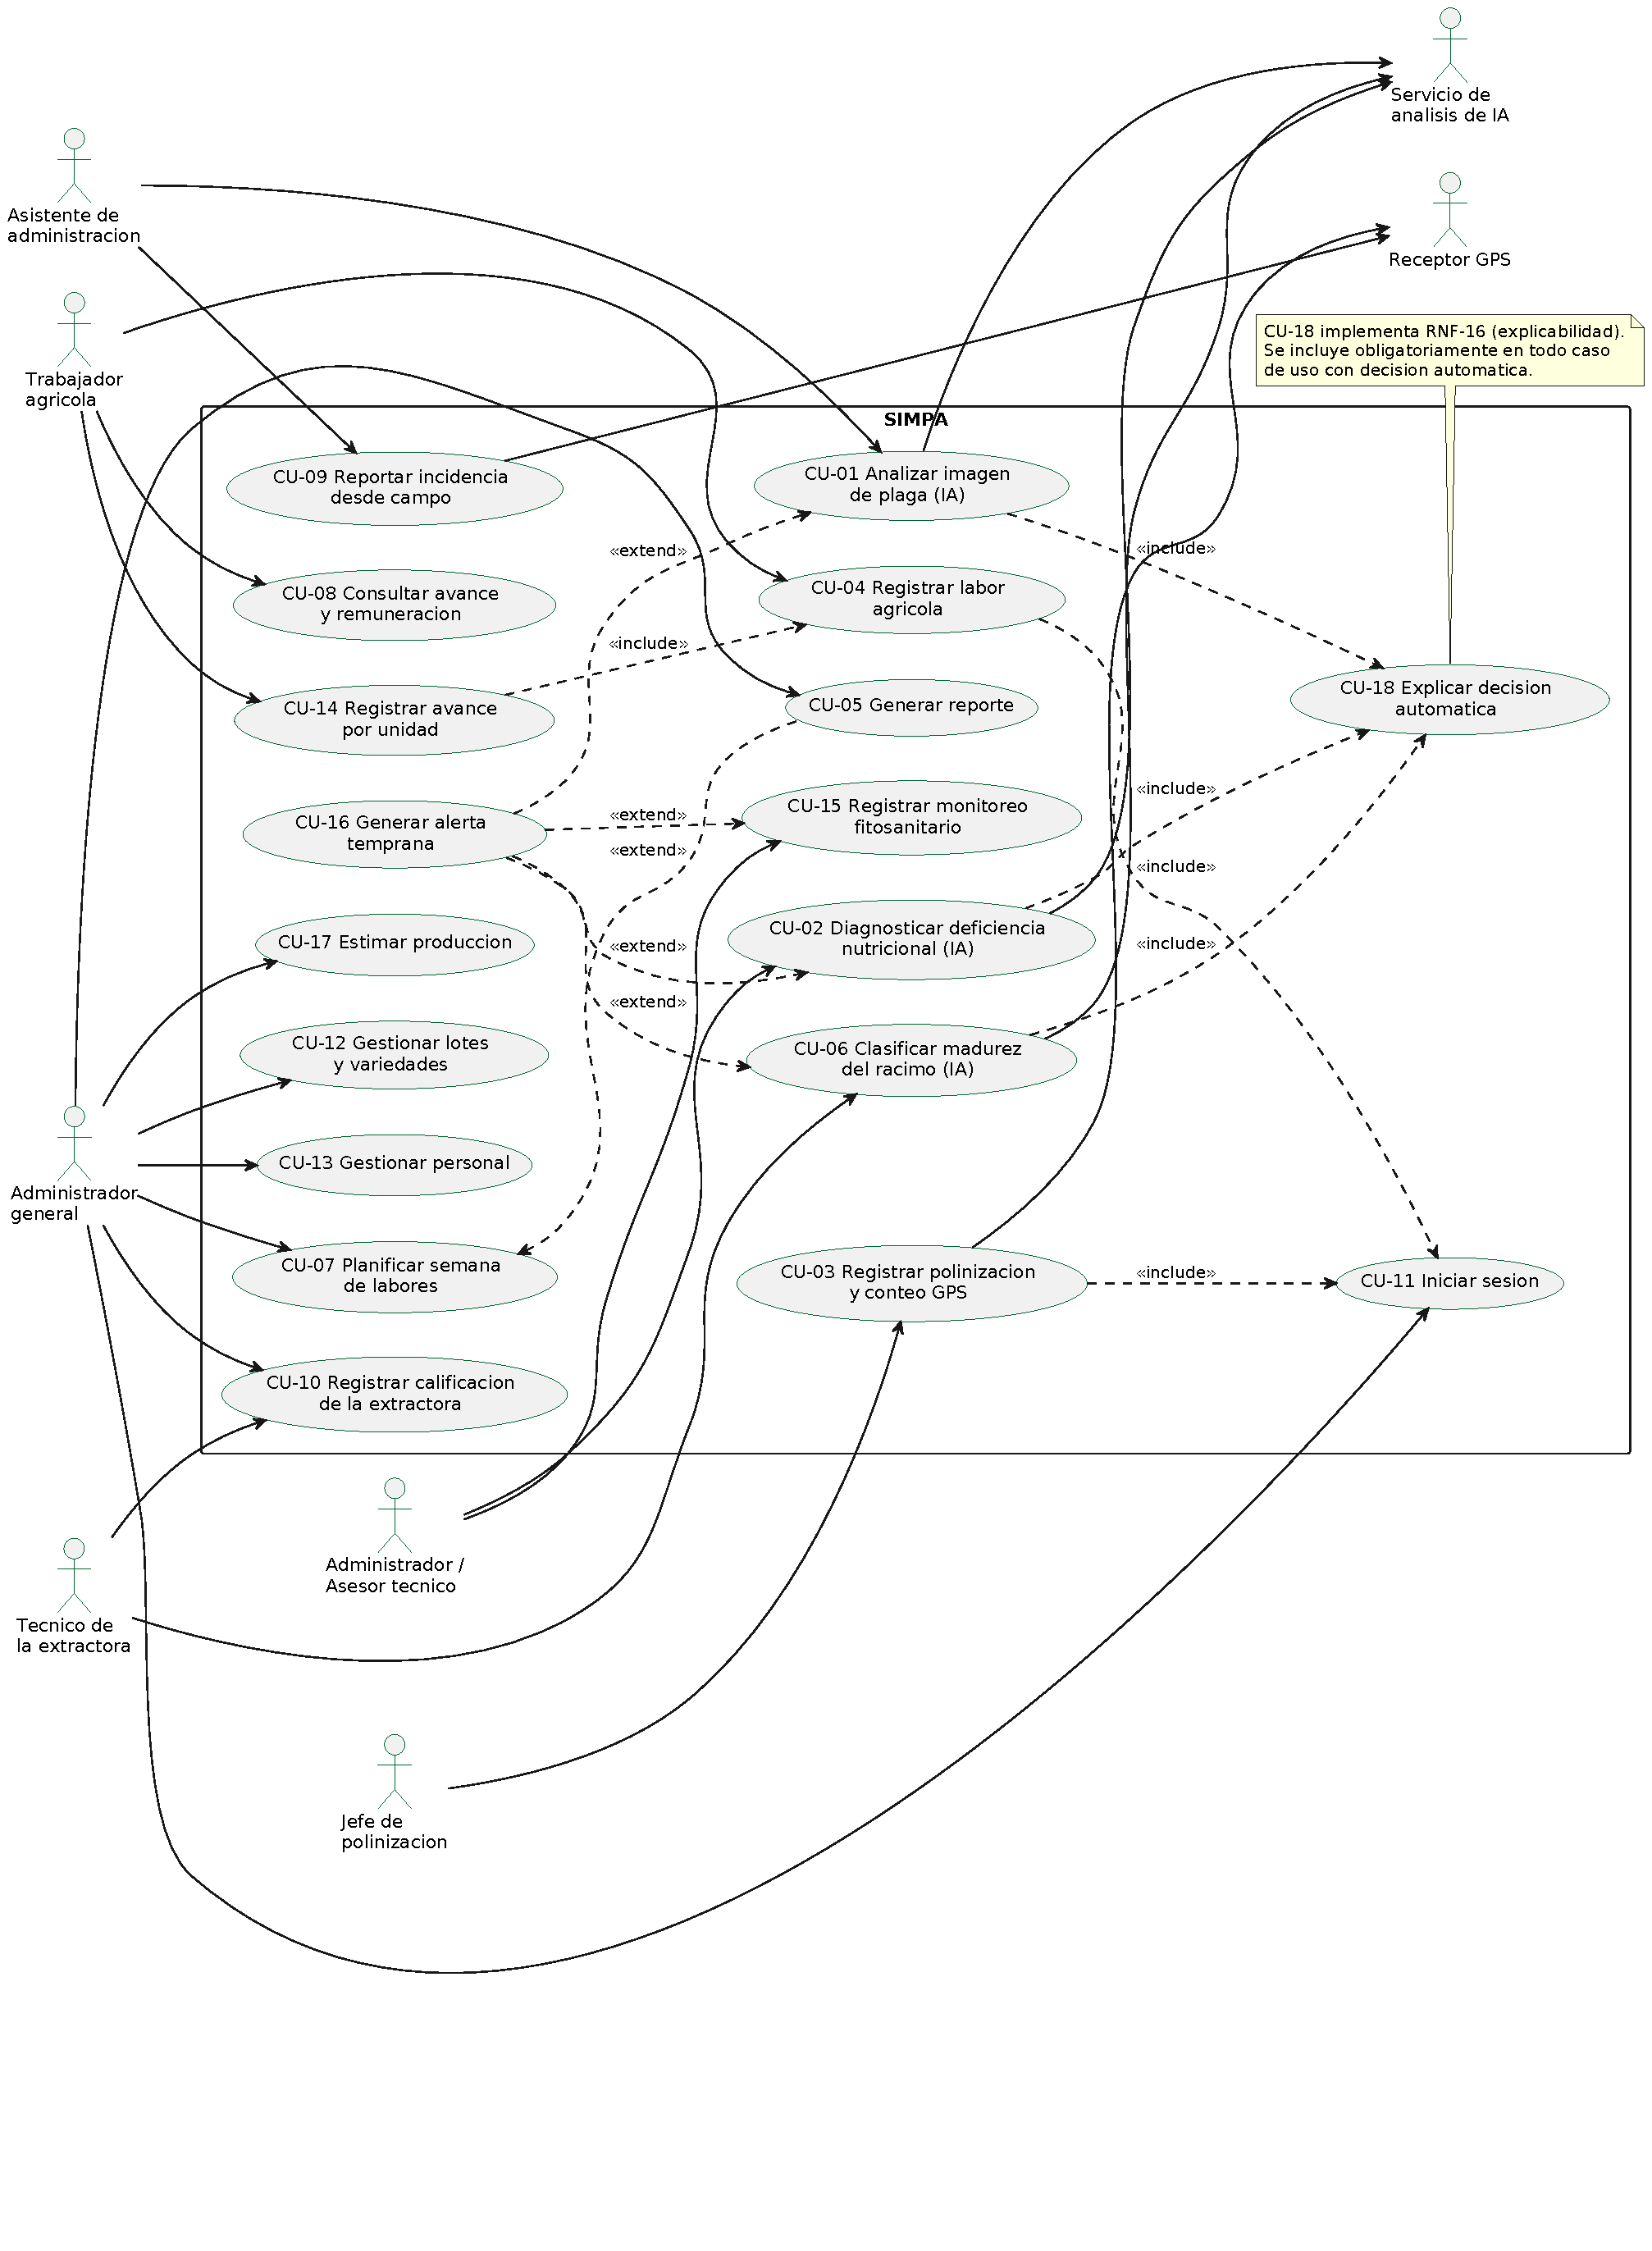
\includegraphics[width=0.91\textwidth]{img/casos_uso_general}
\caption{Diagrama general de casos de uso del SIMPA, con los ocho actores y el límite del sistema.}
\label{fig:cu_general}
\end{figure}

\noindent\textbf{Relaciones de inclusión y extensión.} \id{CU-14} incluye a \id{CU-04}, dado que el
registro de avance presupone una labor registrada. \id{CU-04} y \id{CU-03} incluyen a \id{CU-11},
por requerir sesión autenticada. Los tres casos de uso con decisión automática ---\id{CU-01},
\id{CU-02} y \id{CU-06}--- incluyen obligatoriamente a \id{CU-18}, que materializa el requisito de
explicabilidad \id{RNF-16}: no existe decisión automática sin explicación asociada. \id{CU-16}
extiende a los casos de diagnóstico y de monitoreo, puesto que la alerta se genera únicamente si el
resultado es positivo.

% ---------------------------------------------------------------------
\subsection{Especificación textual de los casos de uso}

Se especifican diez casos de uso, correspondientes a la totalidad de los requisitos funcionales de
prioridad \emph{Must}. Cada especificación incluye actores, precondiciones, postcondiciones, flujo
principal, al menos un flujo alternativo y al menos una excepción.

% --- CU-01
\begin{longtable}{|L{3.4cm}|L{12.0cm}|}
\hline
\rowcolor{grisclaro}\multicolumn{2}{|l|}{\textbf{CU-01 --- Analizar imagen para detectar plaga o enfermedad}}\\
\hline
\textbf{Requisitos} & \id{RF-07}, \id{RF-09}, \id{RF-12}, \id{RNF-16} \\ \hline
\textbf{Actores} & Primario: técnico fitosanitario / asistente de administración. Secundario: servicio de análisis de IA. \\ \hline
\textbf{Precondición} & Persona usuaria autenticada; lote seleccionado; cámara disponible. \\ \hline
\textbf{Postcondición} & El diagnóstico y su explicación quedan registrados y asociados al lote y a la fecha. \\ \hline
\textbf{Flujo principal} & 1. La persona usuaria selecciona el lote y la opción \emph{Analizar imagen}. \newline 2. Captura la fotografía de la palma o de la hoja. \newline 3. El sistema valida la calidad de la imagen. \newline 4. El sistema envía la imagen al servicio de IA con los parámetros de la variedad del lote. \newline 5. El servicio devuelve la clase de afectación, el nivel de confianza y el rasgo visual determinante. \newline 6. El sistema genera la explicación conforme a \id{RNF-16}. \newline 7. El sistema muestra el resultado, la explicación y la recomendación de control, y registra el diagnóstico. \\ \hline
\textbf{Flujo alternativo A} & \emph{Sin conectividad.} En el paso 4 el sistema almacena la imagen localmente y encola el análisis; al restablecerse la conexión lo ejecuta y notifica el resultado (\id{RNF-11}). \\ \hline
\textbf{Flujo alternativo B} & \emph{Confianza insuficiente.} Si el nivel de confianza es inferior al umbral configurado, el sistema no emite clasificación: informa que el resultado no es concluyente y sugiere repetir la captura o consultar a la asesoría técnica. \\ \hline
\textbf{Excepción E1} & Imagen de calidad insuficiente: el sistema solicita repetir la captura indicando el defecto detectado. \\ \hline
\textbf{Excepción E2} & Servicio de IA no disponible: el análisis queda en estado pendiente y la persona usuaria es notificada. \\ \hline
\textbf{Extensión} & Si el resultado es positivo, se ejecuta \id{CU-16} (generar alerta temprana). \\ \hline
\caption{CU-01 --- Analizar imagen para detectar plaga o enfermedad}
\end{longtable}

% --- CU-02
\begin{longtable}{|L{3.4cm}|L{12.0cm}|}
\hline
\rowcolor{grisclaro}\multicolumn{2}{|l|}{\textbf{CU-02 --- Diagnosticar deficiencia nutricional por imagen}}\\
\hline
\textbf{Requisitos} & \id{RF-08}, \id{RF-11}, \id{RNF-16} \\ \hline
\textbf{Actores} & Primario: administrador / asesor técnico. Secundario: servicio de análisis de IA. \\ \hline
\textbf{Precondición} & Persona usuaria autenticada; lote seleccionado con variedad asignada. \\ \hline
\textbf{Postcondición} & El diagnóstico nutricional y su recomendación quedan registrados en el historial del lote. \\ \hline
\textbf{Flujo principal} & 1. La persona usuaria selecciona \emph{Diagnóstico nutricional} y el lote. \newline 2. Captura la fotografía de la hoja. \newline 3. El sistema valida la imagen y la envía al servicio de IA. \newline 4. El servicio estima el elemento deficiente. \newline 5. El sistema genera una explicación de tipo causal, indicando qué signo foliar sustenta la estimación. \newline 6. El sistema muestra la deficiencia, la recomendación de fertilización y la explicación, y registra el diagnóstico. \\ \hline
\textbf{Flujo alternativo A} & La persona usuaria adjunta una imagen existente de la galería en lugar de capturarla. \\ \hline
\textbf{Flujo alternativo B} & \emph{Contraste con análisis de laboratorio.} Si el lote tiene un análisis de suelo o foliar registrado (\id{RF-11}), el sistema contrasta la estimación con los valores medidos y señala la discrepancia si la hubiere. \\ \hline
\textbf{Excepción E1} & Imagen no válida: el sistema solicita repetir la captura. \\ \hline
\textbf{Excepción E2} & Lote sin variedad asignada: el sistema advierte que la estimación puede no ser aplicable y solicita completar el dato. \\ \hline
\textbf{Extensión} & Si la deficiencia estimada es severa, se ejecuta \id{CU-16}. \\ \hline
\caption{CU-02 --- Diagnosticar deficiencia nutricional por imagen}
\end{longtable}

% --- CU-03
\begin{longtable}{|L{3.4cm}|L{12.0cm}|}
\hline
\rowcolor{grisclaro}\multicolumn{2}{|l|}{\textbf{CU-03 --- Registrar polinización y conteo georreferenciado}}\\
\hline
\textbf{Requisitos} & \id{RF-13}, \id{RF-14}, \id{RNF-05}, \id{RNF-12}, \id{RL-03} \\ \hline
\textbf{Actores} & Primario: polinizador. Secundario: receptor GPS. \\ \hline
\textbf{Precondición} & Lote en etapa de polinización; sesión iniciada; consentimiento de geolocalización vigente. \\ \hline
\textbf{Postcondición} & La polinización y el conteo diario quedan registrados por persona, lote y fecha, sin ingreso manual planta por planta. \\ \hline
\textbf{Flujo principal} & 1. El polinizador inicia la jornada en el lote. \newline 2. El sistema verifica la vigencia del consentimiento de geolocalización. \newline 3. El sistema activa el rastreo con período de muestreo de 30 s. \newline 4. Durante la jornada, el sistema almacena las marcaciones georreferenciadas. \newline 5. El polinizador registra el estado de la antesis y la verificación visual. \newline 6. Al cierre, el sistema calcula el número de flores polinizadas a partir de las marcaciones. \newline 7. El sistema almacena el registro y muestra el total a la persona trabajadora. \\ \hline
\textbf{Flujo alternativo A} & \emph{Consentimiento revocado.} Si el consentimiento no está vigente, el sistema no activa el rastreo y habilita el registro manual del número de flores, sin penalización para la persona trabajadora (\id{RL-03}). \\ \hline
\textbf{Flujo alternativo B} & \emph{Sin conectividad.} Las marcaciones se almacenan localmente y se sincronizan al reconectar (\id{RNF-11}). \\ \hline
\textbf{Excepción E1} & Precisión GPS superior a 10 m: el sistema conserva el dato marcándolo como de precisión degradada y advierte a la persona usuaria, sin descartar la jornada (\id{RNF-12}). \\ \hline
\textbf{Excepción E2} & Pérdida total de señal GPS durante la jornada: el sistema conserva el tramo registrado y solicita completar el conteo de forma manual para el tramo faltante. \\ \hline
\caption{CU-03 --- Registrar polinización y conteo georreferenciado}
\end{longtable}

% --- CU-04
\begin{longtable}{|L{3.4cm}|L{12.0cm}|}
\hline
\rowcolor{grisclaro}\multicolumn{2}{|l|}{\textbf{CU-04 --- Registrar labor agrícola}}\\
\hline
\textbf{Requisitos} & \id{RF-04}, \id{RF-28}, \id{RF-35} \\ \hline
\textbf{Actores} & Primario: trabajador agrícola. Alternativo: jefe de campo (registro delegado). \\ \hline
\textbf{Precondición} & Lote y persona trabajadora registrados; persona usuaria autenticada. \\ \hline
\textbf{Postcondición} & La labor y su avance quedan en el historial del lote y computan para el cumplimiento del plan semanal. \\ \hline
\textbf{Flujo principal} & 1. La persona usuaria selecciona el lote y el tipo de labor. \newline 2. Ingresa la cantidad ejecutada en la unidad correspondiente. \newline 3. El sistema valida que la unidad corresponda al tipo de labor. \newline 4. El sistema registra la labor asociada al lote, la fecha y la persona responsable. \newline 5. El sistema actualiza el avance acumulado del período y el cumplimiento de la meta semanal. \\ \hline
\textbf{Flujo alternativo A} & \emph{Registro delegado.} Si la persona trabajadora no dispone de dispositivo propio, el jefe de campo registra el avance en su nombre; el sistema conserva en bitácora la identidad de quien efectuó el registro (\id{RF-35}, \id{RD-10}). \\ \hline
\textbf{Flujo alternativo B} & \emph{Sin conectividad.} La labor se almacena localmente y se sincroniza al reconectar. \\ \hline
\textbf{Excepción E1} & Datos incompletos: el sistema impide guardar y señala los campos faltantes. \\ \hline
\textbf{Excepción E2} & Unidad incompatible con el tipo de labor: el sistema rechaza el registro e indica la unidad esperada. \\ \hline
\caption{CU-04 --- Registrar labor agrícola}
\end{longtable}

% --- CU-05
\begin{longtable}{|L{3.4cm}|L{12.0cm}|}
\hline
\rowcolor{grisclaro}\multicolumn{2}{|l|}{\textbf{CU-05 --- Generar reporte}}\\
\hline
\textbf{Requisitos} & \id{RF-19}, \id{RF-26} \\ \hline
\textbf{Actores} & Primario: administrador general. \\ \hline
\textbf{Precondición} & Existen registros en el período seleccionado. \\ \hline
\textbf{Postcondición} & El reporte queda disponible para consulta o exportación. \\ \hline
\textbf{Flujo principal} & 1. La persona administradora selecciona el tipo de reporte y el período. \newline 2. El sistema consolida labores, avance, producción y alertas del período. \newline 3. El sistema genera y presenta el reporte. \newline 4. La persona administradora lo consulta o lo exporta a PDF o a hoja de cálculo. \\ \hline
\textbf{Flujo alternativo A} & Filtrado por lote, por equipo o por persona trabajadora. \\ \hline
\textbf{Flujo alternativo B} & \emph{Reporte de cumplimiento semanal.} El sistema contrasta el plan de la semana con lo ejecutado y destaca las metas no alcanzadas y su remanente. \\ \hline
\textbf{Excepción E1} & Sin registros en el período: el sistema informa la ausencia de datos y propone un período alternativo con información disponible. \\ \hline
\caption{CU-05 --- Generar reporte}
\end{longtable}

% --- CU-06
\begin{longtable}{|L{3.4cm}|L{12.0cm}|}
\hline
\rowcolor{grisclaro}\multicolumn{2}{|l|}{\textbf{CU-06 --- Clasificar la madurez del racimo}}\\
\hline
\textbf{Requisitos} & \id{RF-21}, \id{RF-22}, \id{RD-07}, \id{RD-08}, \id{RNF-01}, \id{RNF-16} \\ \hline
\textbf{Actores} & Primario: cosechador / técnico de la extractora. Secundario: servicio de análisis de IA. \\ \hline
\textbf{Precondición} & Lote con variedad asignada; persona usuaria autenticada. \\ \hline
\textbf{Postcondición} & La clasificación queda asociada al racimo, al lote y a la fecha, y actualiza el porcentaje estimado de fruta verde del lote. \\ \hline
\textbf{Flujo principal} & 1. La persona usuaria selecciona el lote y la opción \emph{Clasificar racimo}. \newline 2. El sistema recupera el umbral de desprendimiento de la variedad del lote. \newline 3. La persona usuaria captura la fotografía de la parte basal del racimo. \newline 4. El servicio de IA cuenta los frutos desprendidos, sin emplear el color como criterio (\id{RD-07}). \newline 5. El sistema compara el conteo con el umbral de la variedad y determina el estado. \newline 6. El sistema genera una explicación por contraste, indicando el conteo obtenido y el umbral aplicable. \newline 7. El sistema registra la clasificación y actualiza el porcentaje de fruta verde del lote. \\ \hline
\textbf{Flujo alternativo A} & \emph{Verificación previa al despacho.} La persona usuaria solicita el porcentaje estimado de fruta verde del lote; si alcanza o supera el umbral de penalización, el sistema emite alerta preventiva y desaconseja el despacho (\id{RF-22}). \\ \hline
\textbf{Flujo alternativo B} & \emph{Sobremadurez.} Si el conteo excede ampliamente el umbral, el sistema clasifica el racimo como sobremaduro y advierte sobre el incremento de acidez. \\ \hline
\textbf{Excepción E1} & Lote sin variedad asignada: el sistema no clasifica y solicita completar el dato, dado que el umbral depende de la variedad. \\ \hline
\textbf{Excepción E2} & Parte basal no visible en la imagen: el sistema solicita repetir la captura indicando el encuadre requerido. \\ \hline
\caption{CU-06 --- Clasificar la madurez del racimo}
\end{longtable}

% --- CU-07
\begin{longtable}{|L{3.4cm}|L{12.0cm}|}
\hline
\rowcolor{grisclaro}\multicolumn{2}{|l|}{\textbf{CU-07 --- Planificar la semana de labores}}\\
\hline
\textbf{Requisitos} & \id{RF-26}, \id{RF-27}, \id{RF-34}, \id{RF-37} a \id{RF-39} \\ \hline
\textbf{Actores} & Primario: administrador general. \\ \hline
\textbf{Precondición} & Lotes y tipos de labor registrados. \\ \hline
\textbf{Postcondición} & El plan de la semana queda publicado y disponible para el seguimiento diario. \\ \hline
\textbf{Flujo principal} & 1. La persona administradora crea el plan de la semana. \newline 2. Para cada lote, define las labores previstas con su meta y unidad. \newline 3. El sistema incorpora automáticamente los remanentes arrastrados de la semana anterior. \newline 4. La persona administradora registra los insumos requeridos. \newline 5. El sistema publica el plan y lo hace visible al jefe de campo. \\ \hline
\textbf{Flujo alternativo A} & \emph{Cierre de semana.} Al cierre, el sistema calcula el cumplimiento de cada meta; si es parcial, genera el remanente como labor pendiente de la semana siguiente, vinculada a la de origen (\id{RF-27}). \\ \hline
\textbf{Flujo alternativo B} & Ajuste del plan durante la semana en curso, conservando la versión previa en bitácora. \\ \hline
\textbf{Flujo alternativo C} & \emph{Liquidación y aprobación.} Al cierre, el sistema genera la liquidación que contrasta cantidad presupuestada, cantidad ejecutada, tarifa y valor por grupo de labor, totaliza el gasto presupuestado frente al real, e incorpora las labores no presupuestadas en su grupo diferenciado (\id{RF-37}, \id{RF-38}). La persona administradora aprueba la liquidación y el período queda cerrado (\id{RF-39}). \\ \hline
\textbf{Excepción E1} & Meta expresada en unidad incompatible con el tipo de labor: el sistema rechaza la meta e indica la unidad esperada. \\ \hline
\textbf{Excepción E2} & Existe un plan publicado para la misma semana: el sistema advierte y solicita confirmación antes de sustituirlo. \\ \hline
\caption{CU-07 --- Planificar la semana de labores}
\end{longtable}

% --- CU-08
\begin{longtable}{|L{3.4cm}|L{12.0cm}|}
\hline
\rowcolor{grisclaro}\multicolumn{2}{|l|}{\textbf{CU-08 --- Consultar avance acumulado y remuneración estimada}}\\
\hline
\textbf{Requisitos} & \id{RF-29}, \id{RF-36}, \id{RL-04} \\ \hline
\textbf{Actores} & Primario: trabajador agrícola. \\ \hline
\textbf{Precondición} & Existen registros de avance de la persona trabajadora en el período. \\ \hline
\textbf{Postcondición} & Se presenta el consolidado del período, sin posibilidad de edición por parte de la persona trabajadora. \\ \hline
\textbf{Flujo principal} & 1. La persona trabajadora accede a \emph{Mi avance}. \newline 2. Selecciona el período (quincena en curso por defecto). \newline 3. El sistema agrega sus registros de avance por tipo de labor. \newline 4. El sistema obtiene del catálogo la tarifa vigente de cada tipo de labor a la fecha de cada registro y calcula la remuneración estimada correspondiente al trabajo por avance. \newline 5. El sistema presenta el desglose por labor y el total estimado. \\ \hline
\textbf{Flujo alternativo A} & \emph{Ejercicio del derecho de acceso.} La persona trabajadora solicita la exportación de sus datos personales; el sistema genera el archivo conforme al Art. 12 de la LOPDP (\id{RL-04}). \\ \hline
\textbf{Flujo alternativo B} & \emph{Discrepancia.} La persona trabajadora marca un registro como discrepante; el sistema notifica a la administración sin modificar el dato original, y la corrección se tramita mediante \id{RL-05}. \\ \hline
\textbf{Excepción E1} & Sin registros en el período: el sistema informa la ausencia de datos. \\ \hline
\textbf{Excepción E2} & La labor carece de tarifa vigente en el catálogo (\id{RF-36}) a la fecha del registro: el sistema muestra el avance en unidades, omite la estimación monetaria e indica que la tarifa no está vigente para esa fecha. \\ \hline
\caption{CU-08 --- Consultar avance acumulado y remuneración estimada}
\end{longtable}

% --- CU-09
\begin{longtable}{|L{3.4cm}|L{12.0cm}|}
\hline
\rowcolor{grisclaro}\multicolumn{2}{|l|}{\textbf{CU-09 --- Reportar incidencia desde el campo}}\\
\hline
\textbf{Requisitos} & \id{RF-30}, \id{RF-31}, \id{RF-12} \\ \hline
\textbf{Actores} & Primario: asistente de administración / trabajador agrícola. Secundario: receptor GPS. \\ \hline
\textbf{Precondición} & Persona usuaria autenticada; cámara y GPS disponibles. \\ \hline
\textbf{Postcondición} & La incidencia queda registrada con fotografía y coordenadas, e incorporada a la lista de pendientes de verificación. \\ \hline
\textbf{Flujo principal} & 1. La persona usuaria selecciona \emph{Reportar incidencia}. \newline 2. Captura la fotografía de la afectación. \newline 3. El sistema obtiene las coordenadas del punto. \newline 4. La persona usuaria selecciona el lote y describe la afectación. \newline 5. El sistema registra la incidencia georreferenciada. \newline 6. El sistema la incorpora a la lista de pendientes de la persona supervisora. \\ \hline
\textbf{Flujo alternativo A} & \emph{Análisis asistido.} La persona usuaria solicita el análisis de la fotografía; se ejecuta \id{CU-01} y el diagnóstico se asocia a la incidencia. \\ \hline
\textbf{Flujo alternativo B} & \emph{Verificación en visita.} La persona supervisora recorre su lista de pendientes, ubica la incidencia por sus coordenadas y la marca como verificada o descartada. \\ \hline
\textbf{Excepción E1} & GPS no disponible: el sistema registra la incidencia solicitando la selección manual del lote y la marca como de ubicación aproximada. \\ \hline
\textbf{Excepción E2} & Sin conectividad: la incidencia se encola y se sincroniza al reconectar, conservando el instante original de captura. \\ \hline
\caption{CU-09 --- Reportar incidencia desde el campo}
\end{longtable}

% --- CU-10
\begin{longtable}{|L{3.4cm}|L{12.0cm}|}
\hline
\rowcolor{grisclaro}\multicolumn{2}{|l|}{\textbf{CU-10 --- Registrar la calificación de la planta extractora}}\\
\hline
\textbf{Requisitos} & \id{RF-23}, \id{RF-24}, \id{RF-25}, \id{RF-33} \\ \hline
\textbf{Actores} & Primario: administrador general. \\ \hline
\textbf{Precondición} & Existe un despacho registrado con su fecha de corte. \\ \hline
\textbf{Postcondición} & La calificación queda asociada al lote de origen y disponible para el análisis de trazabilidad. \\ \hline
\textbf{Flujo principal} & 1. La persona administradora selecciona el despacho. \newline 2. Ingresa los datos del ticket de pesaje: peso bruto, tara y neto. \newline 3. Ingresa la calificación de calidad: tamaño del fruto, porcentaje de fruta verde, sobremadura, malformación y pedúnculo largo. \newline 4. El sistema calcula el intervalo entre el corte y la entrega. \newline 5. El sistema registra la calificación y la asocia al lote de origen. \\ \hline
\textbf{Flujo alternativo A} & \emph{Análisis de trazabilidad.} Ante una calificación desfavorable, la persona administradora consulta la cadena lote $\rightarrow$ fecha de corte $\rightarrow$ cuadrilla, y contrasta con las labores del período para distinguir si el origen está en la cosecha o en el manejo del cultivo (\id{RF-24}). \\ \hline
\textbf{Flujo alternativo B} & \emph{Ausencia de guía de remisión.} Si el despacho se registra sin número de guía, el sistema advierte antes del cierre (\id{RF-33}). \\ \hline
\textbf{Excepción E1} & El intervalo entre corte y entrega supera el valor recomendado para la variedad: el sistema registra la advertencia junto al despacho (\id{RF-25}). \\ \hline
\textbf{Excepción E2} & La suma de pesos es inconsistente (neto distinto de bruto menos tara): el sistema rechaza el registro e indica la inconsistencia. \\ \hline
\caption{CU-10 --- Registrar la calificación de la planta extractora}
\end{longtable}

% ---------------------------------------------------------------------
\subsection{Diagrama de clases refinado}

El modelo del dominio comprende veinticinco clases con atributos y operaciones. Incorpora tres
jerarquías de herencia (\id{Persona}--\id{Usuario} y la especialización de \id{Diagnostico} en sus
tres variantes), cuatro relaciones de composición y asociaciones con multiplicidad explícita. No
corresponde a un diseño de base de datos, sino al modelo conceptual del dominio del problema.

\begin{figure}[!htbp]
\centering
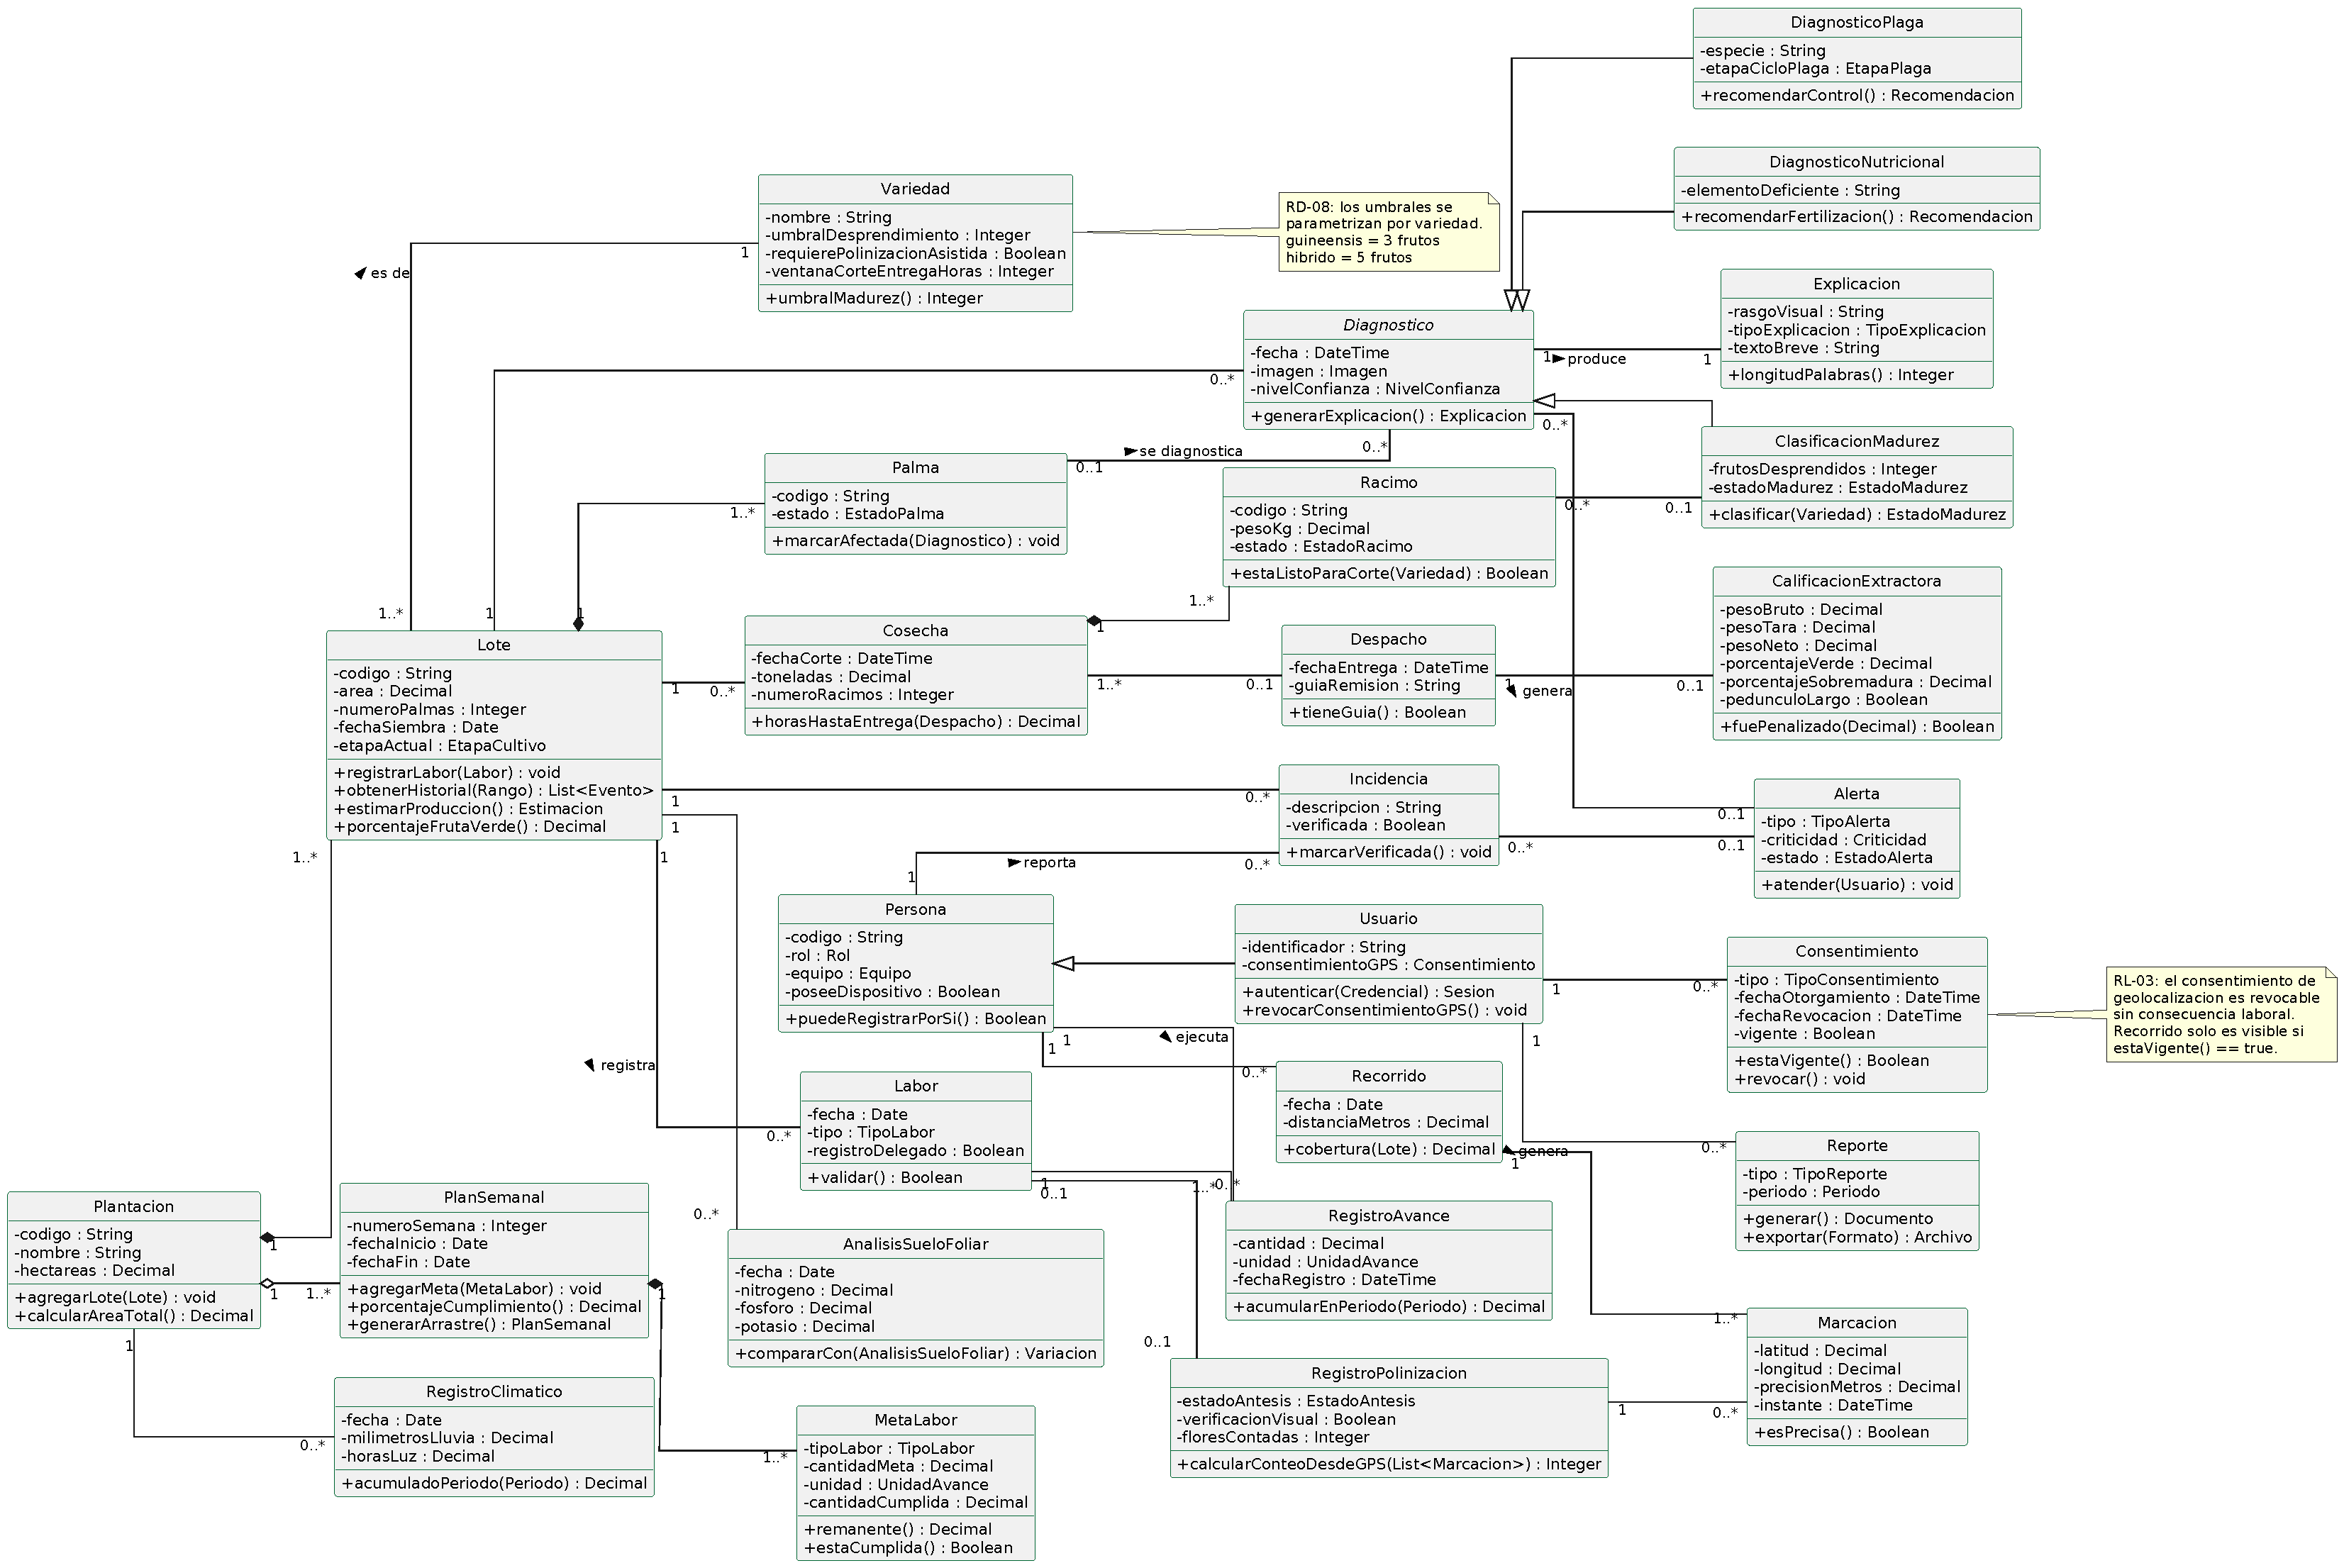
\includegraphics[width=1.0\textwidth]{img/clases_refinado}
\caption{Diagrama de clases refinado del SIMPA, con atributos y operaciones.}
\label{fig:clases}
\end{figure}

\noindent\textbf{Decisiones de modelado relevantes.} La clase \id{Consentimiento} se modela como
entidad de primer orden y no como atributo booleano de \id{Usuario}, porque el Art. 7 de la LOPDP
exige que el consentimiento sea específico por finalidad y revocable, lo que obliga a conservar su
historia. La clase \id{Variedad} concentra los umbrales de decisión ---desprendimiento, ventana
corte-entrega y necesidad de polinización asistida--- en lugar de fijarlos en la lógica de los
módulos de IA, conforme a \id{RD-08}. La clase \id{Explicacion} se asocia de forma obligatoria a
\id{Diagnostico} con multiplicidad 1:1, de modo que el modelo impide estructuralmente la existencia
de una decisión automática sin explicación (\id{RNF-16}). La clase \id{RegistroAvance} se separa de
\id{Labor} porque una labor puede acumular avances de varias personas y días, patrón observado en
los documentos de planificación semanal (\id{EV-11}).

% ---------------------------------------------------------------------
\subsection{Diagramas de secuencia}

Se presentan los diagramas de secuencia de los tres casos de uso \emph{Must} de mayor complejidad
de interacción.

\begin{figure}[!htbp]
\centering
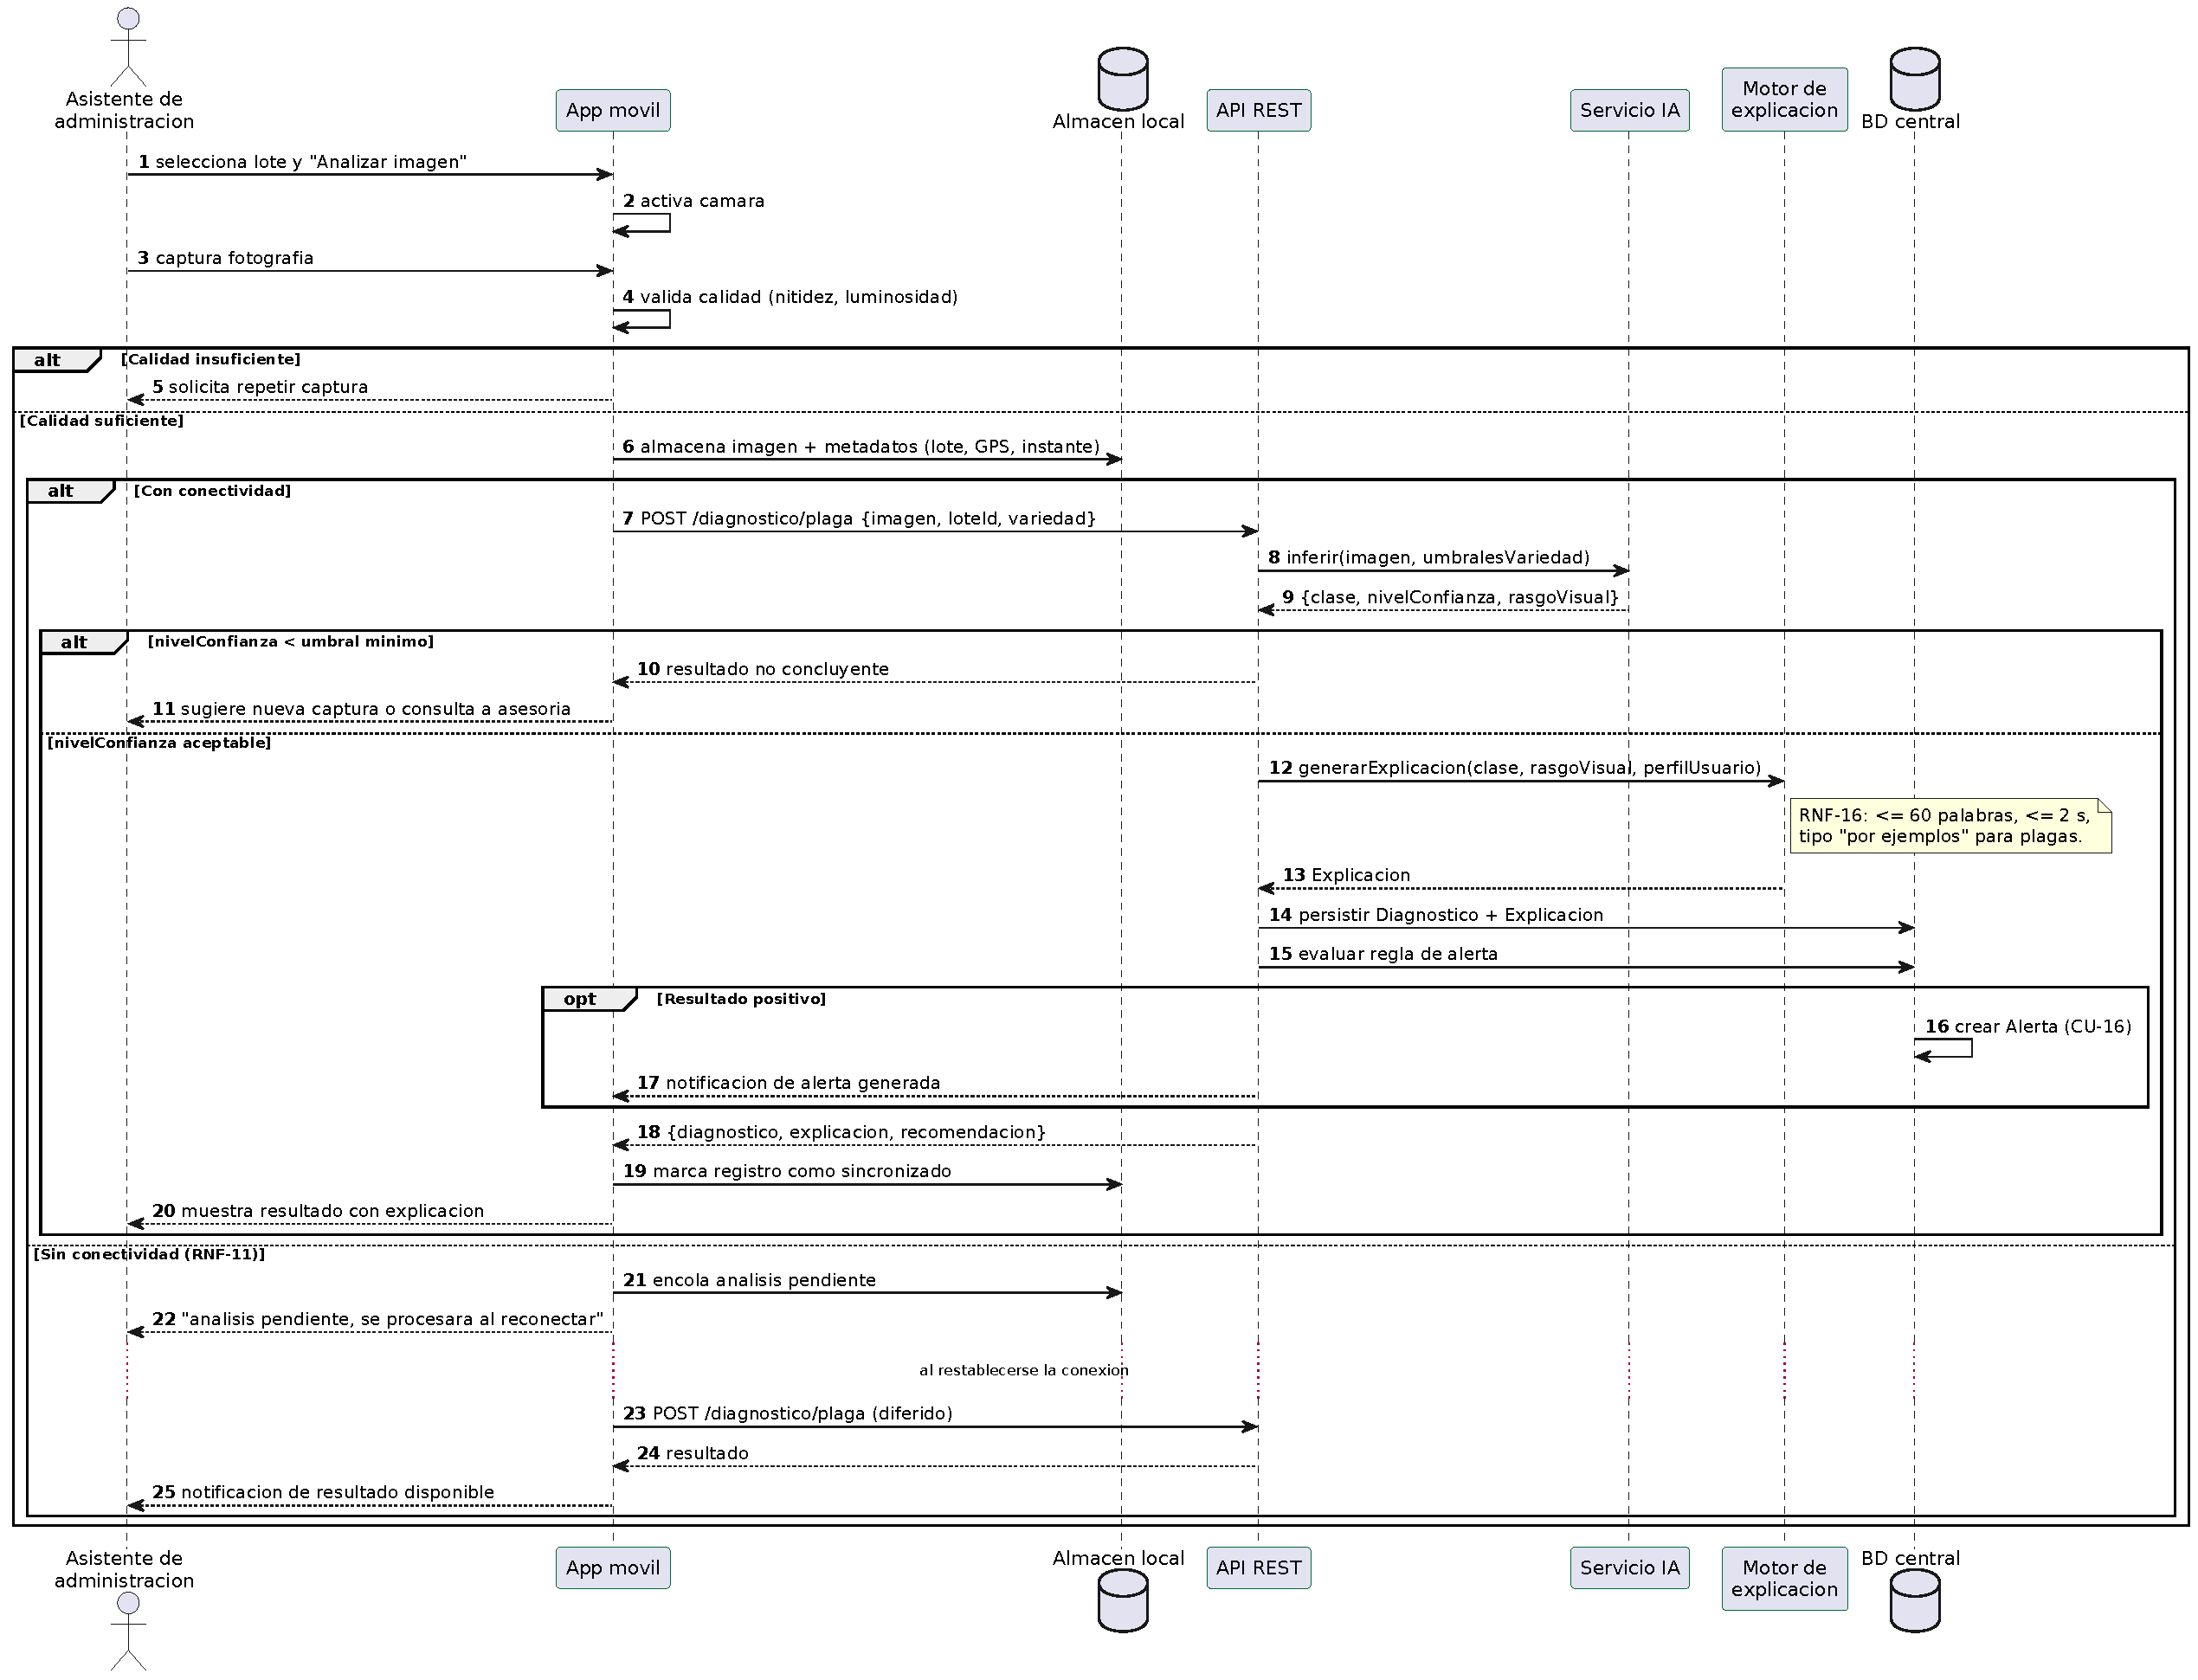
\includegraphics[width=1.0\textwidth]{img/secuencia_CU01}
\caption{Diagrama de secuencia del CU-01: análisis de imagen para detección de plaga, con las ramas de baja confianza y de operación sin conectividad.}
\label{fig:seq01}
\end{figure}

\begin{figure}[!htbp]
\centering
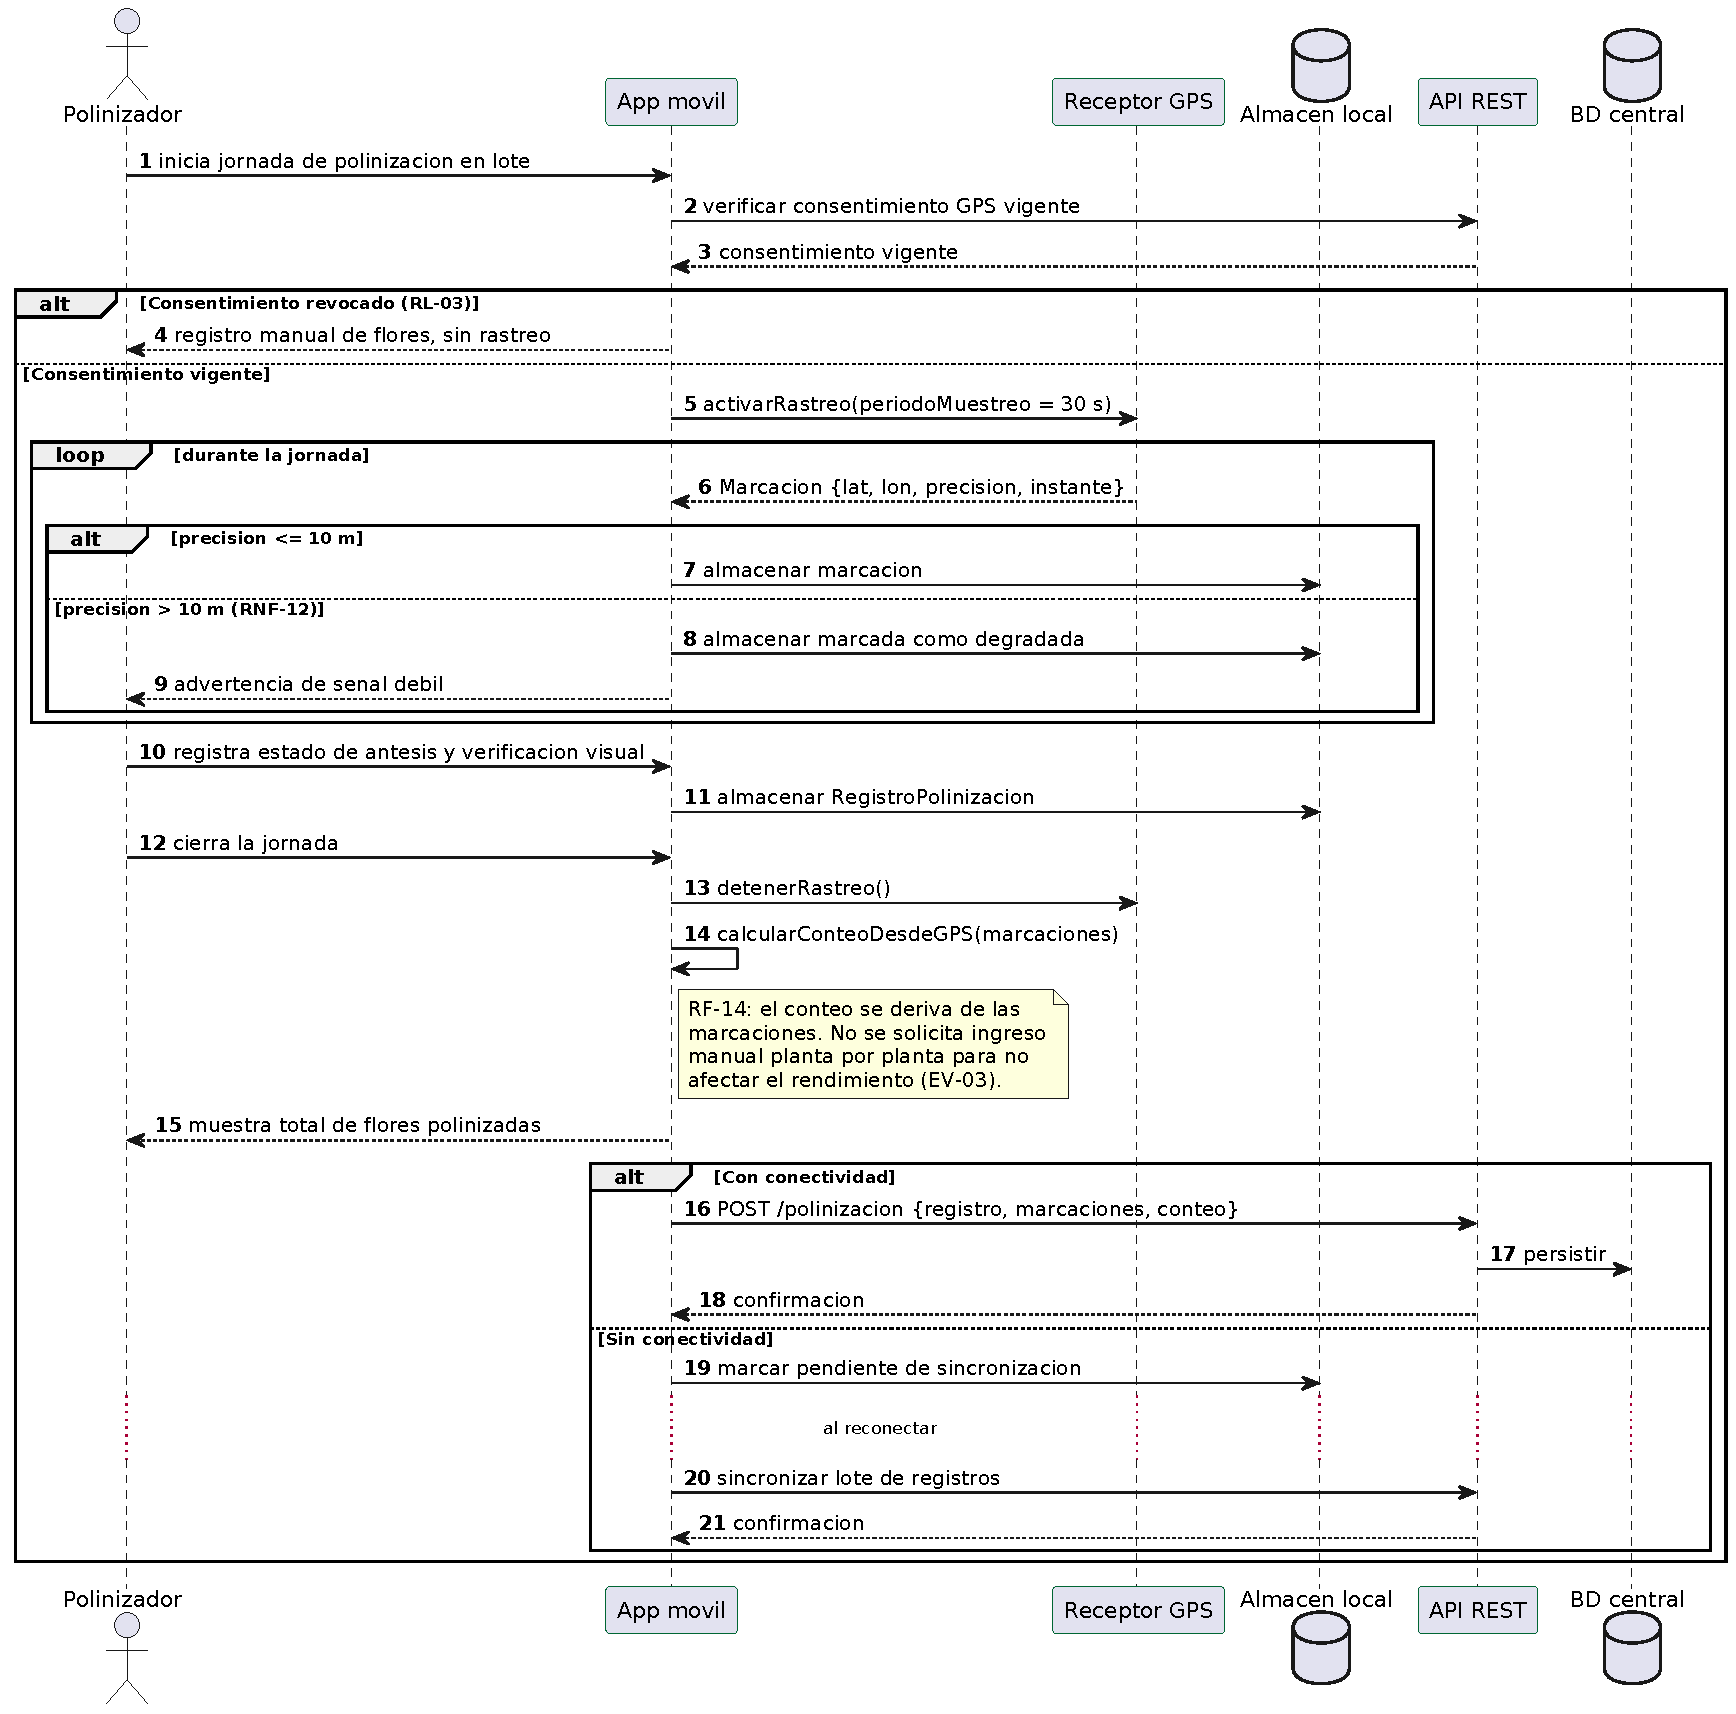
\includegraphics[width=1.0\textwidth]{img/secuencia_CU03}
\caption{Diagrama de secuencia del CU-03: registro de polinización y conteo georreferenciado, con verificación de consentimiento y manejo de precisión degradada.}
\label{fig:seq03}
\end{figure}

\begin{figure}[!htbp]
\centering
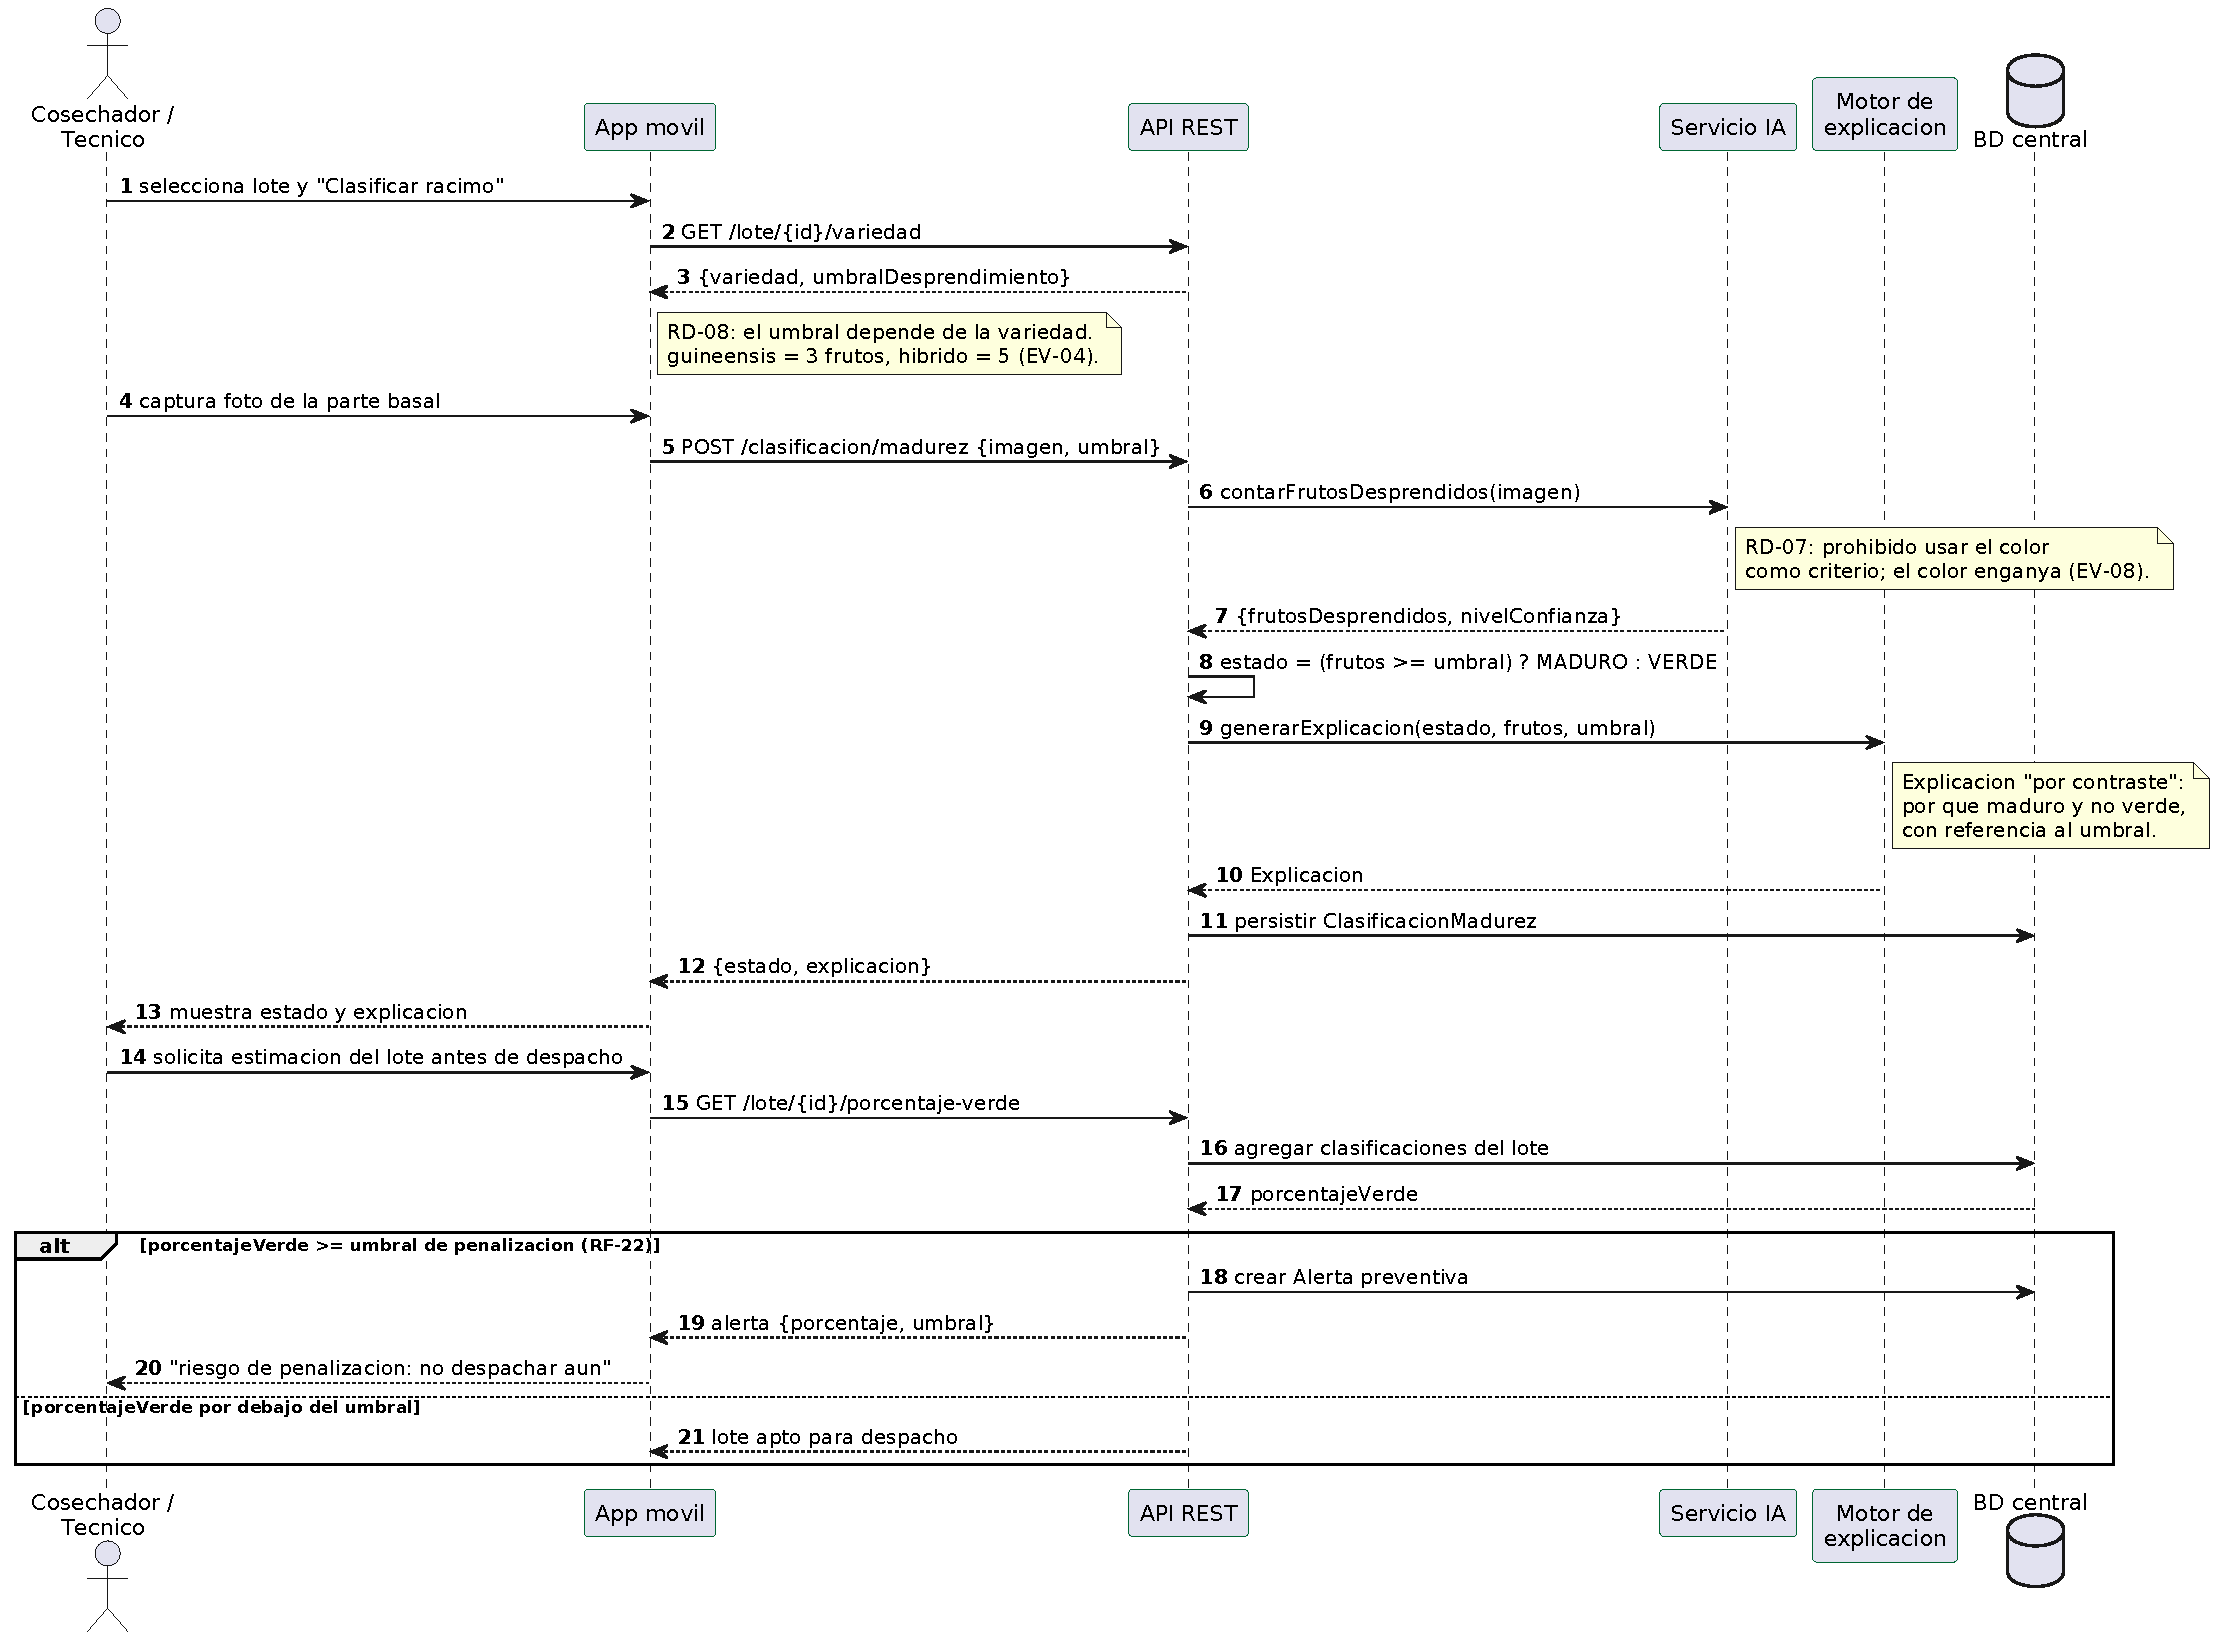
\includegraphics[width=1.0\textwidth]{img/secuencia_CU06}
\caption{Diagrama de secuencia del CU-06: clasificación de madurez del racimo y alerta preventiva de porcentaje de fruta verde.}
\label{fig:seq06}
\end{figure}

% ---------------------------------------------------------------------
\subsection{Diagrama de actividad}

El diagrama modela el ciclo semanal completo de planificación y ejecución, que constituye el proceso
central de la organización según los documentos operativos (\id{EV-11}). Incorpora la bifurcación
por disponibilidad de dispositivo (\id{RF-35}), la bifurcación por conectividad (\id{RNF-11}) y el
mecanismo de arrastre de labor incompleta (\id{RF-27}).

\begin{figure}[!htbp]
\centering
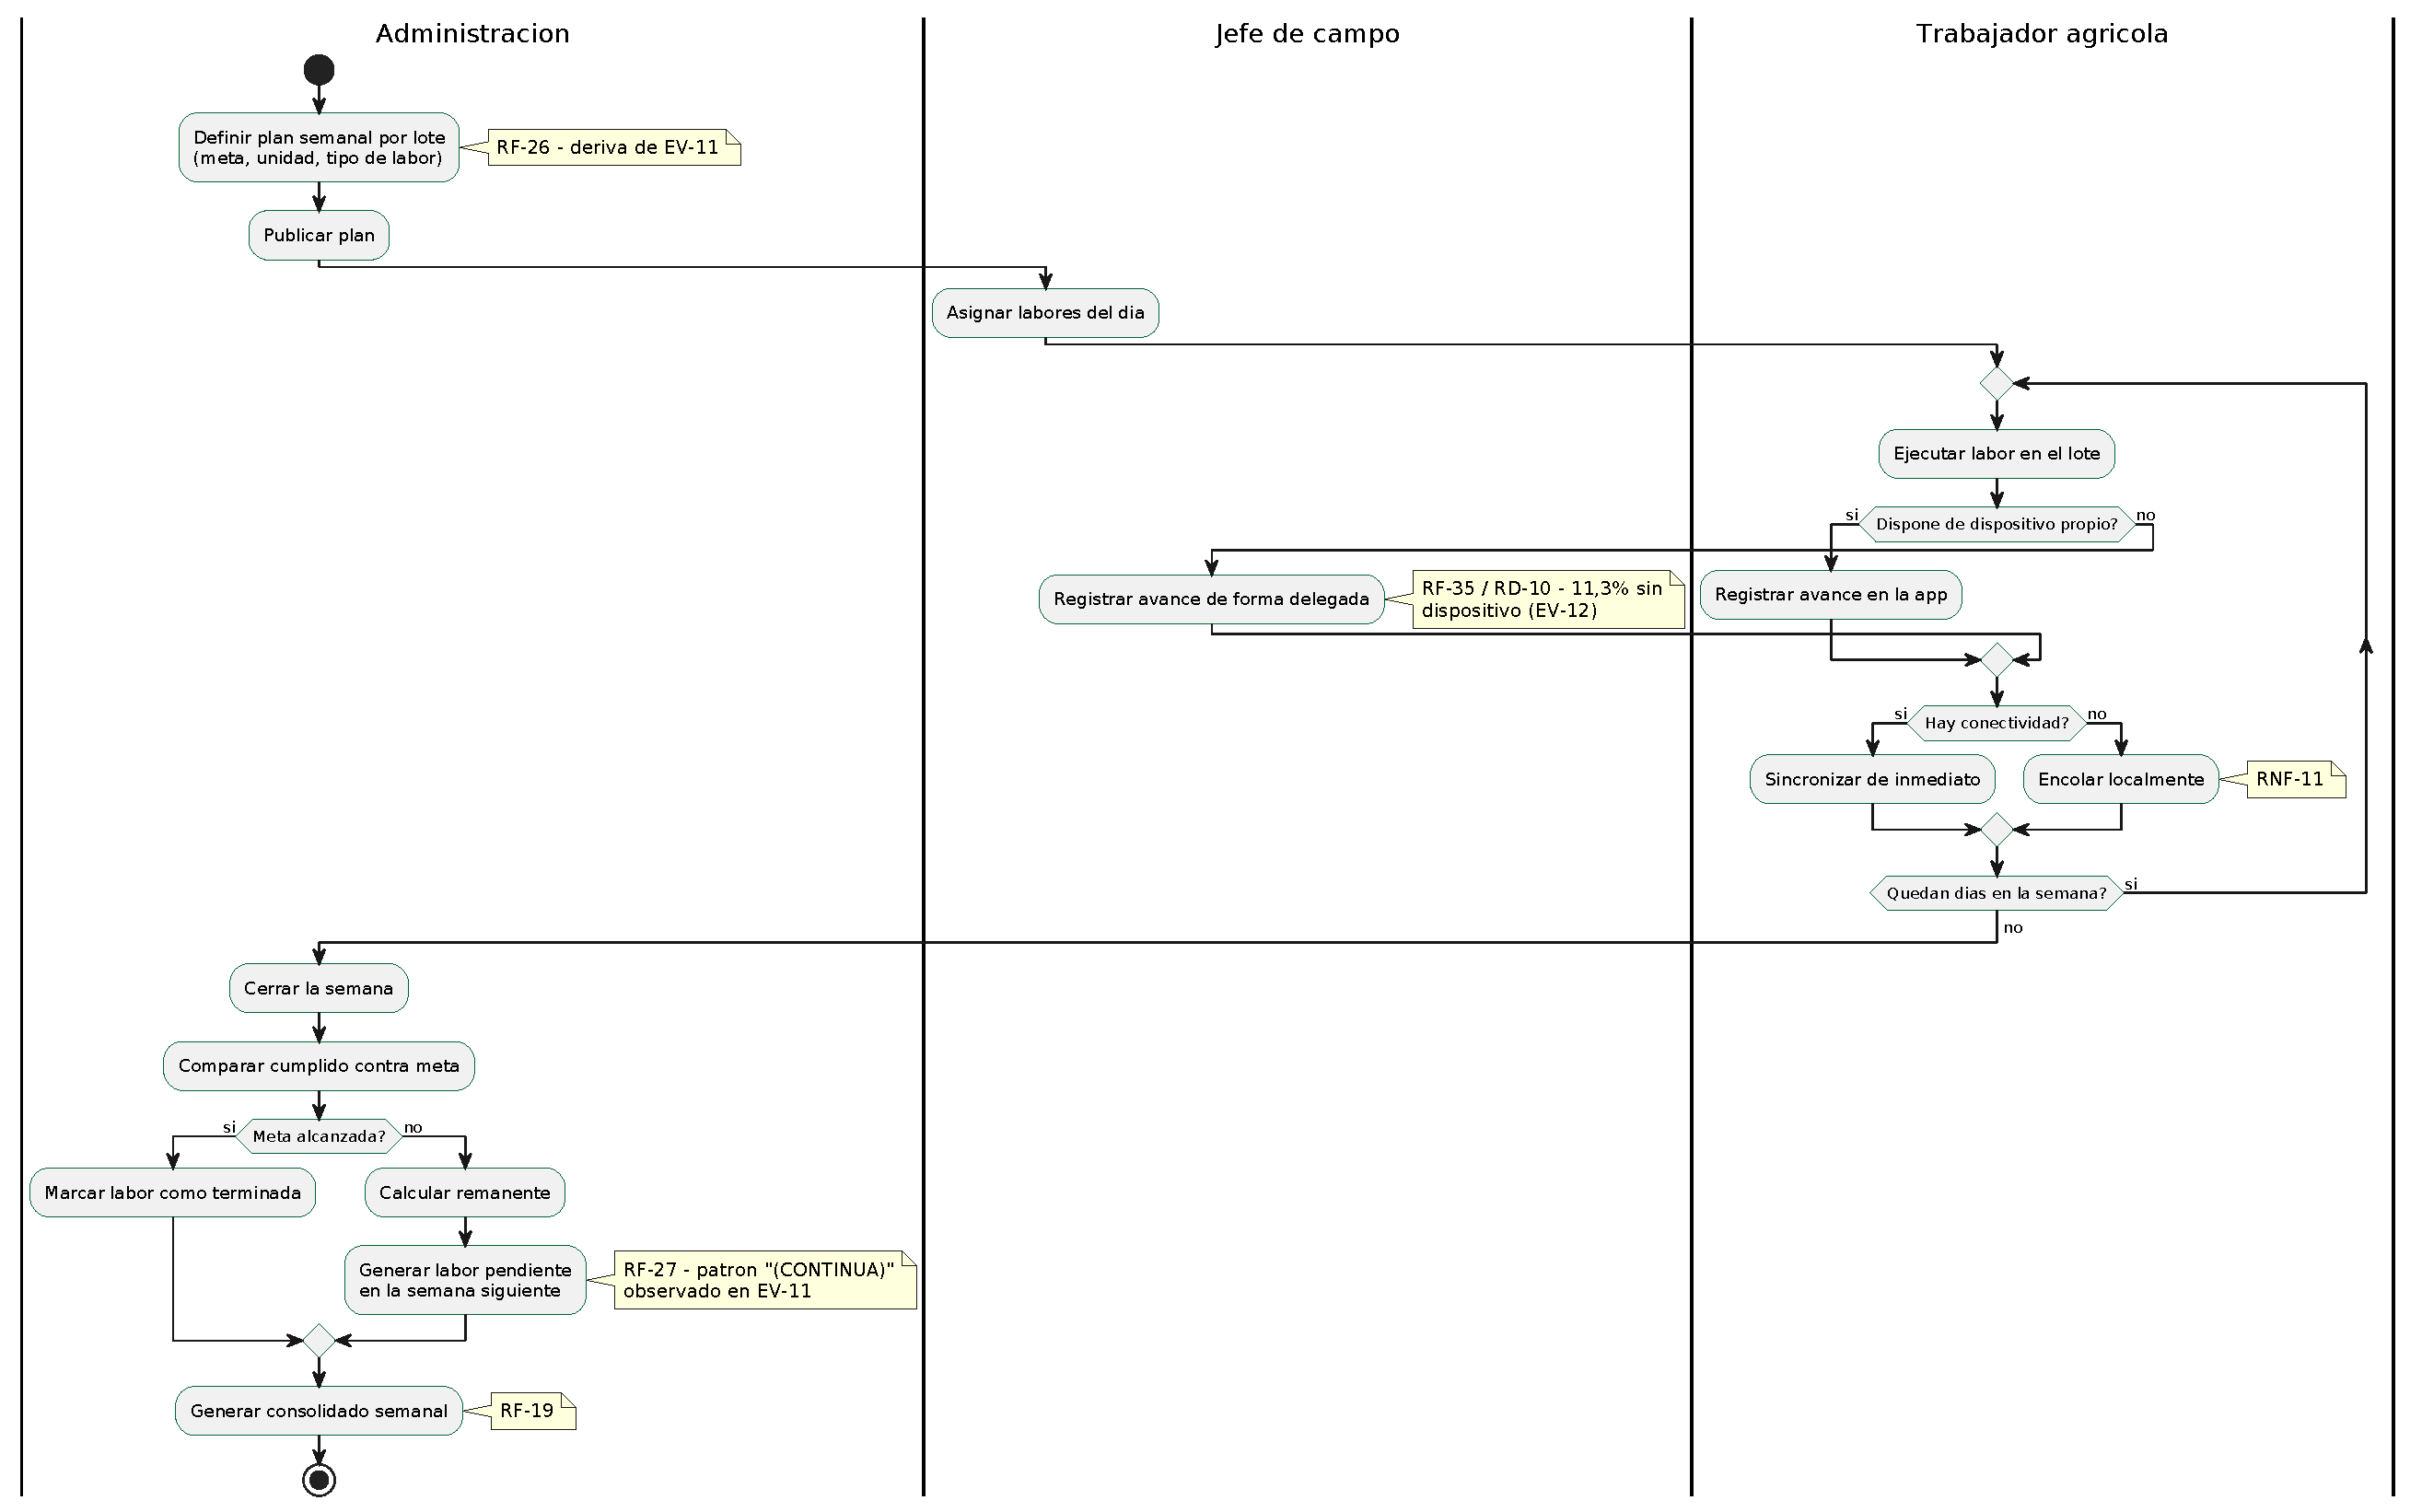
\includegraphics[width=1.0\textwidth]{img/actividad_ciclo_semanal}
\caption{Diagrama de actividad del ciclo semanal de planificación y ejecución de labores.}
\label{fig:actividad}
\end{figure}

% ---------------------------------------------------------------------
\subsection{Diagramas de estados}

Se modelan las dos entidades del dominio con ciclo de vida no trivial: el \textbf{racimo}, cuya
trayectoria determina el valor económico de la producción, y la \textbf{alerta}, cuyo ciclo refleja
la latencia real de verificación documentada en \id{EV-07}.

\begin{figure}[!htbp]
\centering
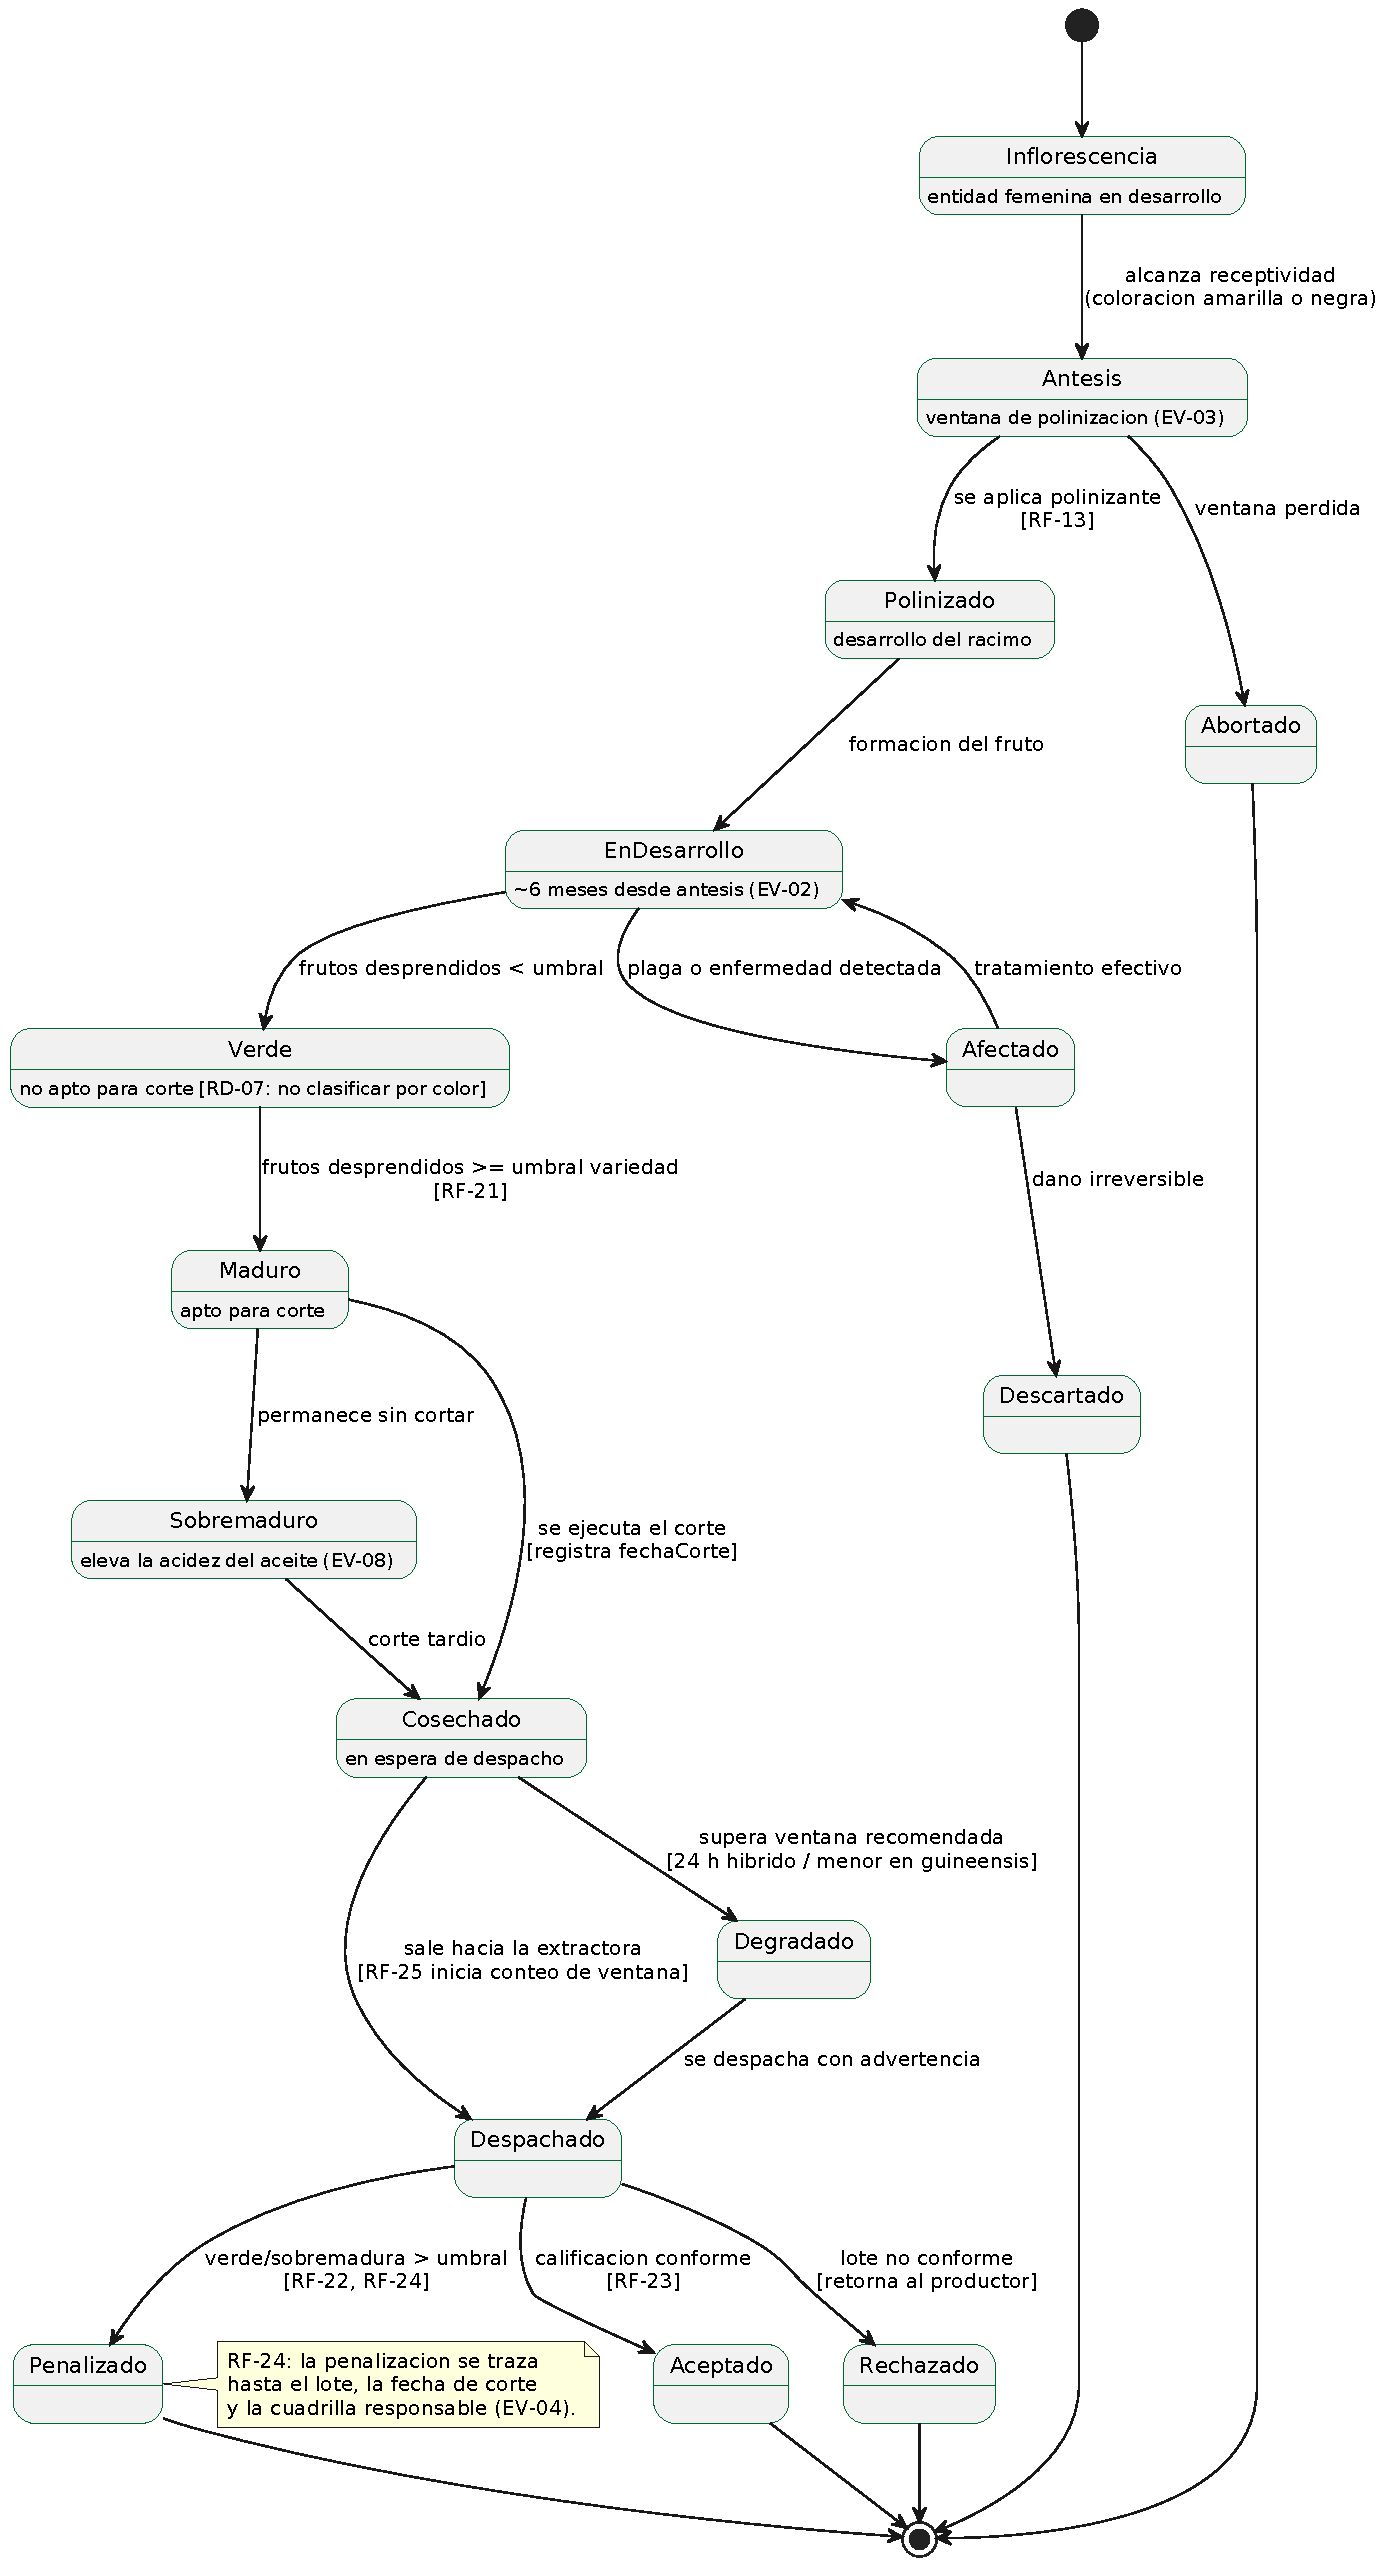
\includegraphics[width=0.67\textwidth]{img/estados_racimo}
\caption{Diagrama de estados del racimo, desde la inflorescencia hasta la calificación en la planta extractora.}
\label{fig:est_racimo}
\end{figure}

\begin{figure}[!htbp]
\centering
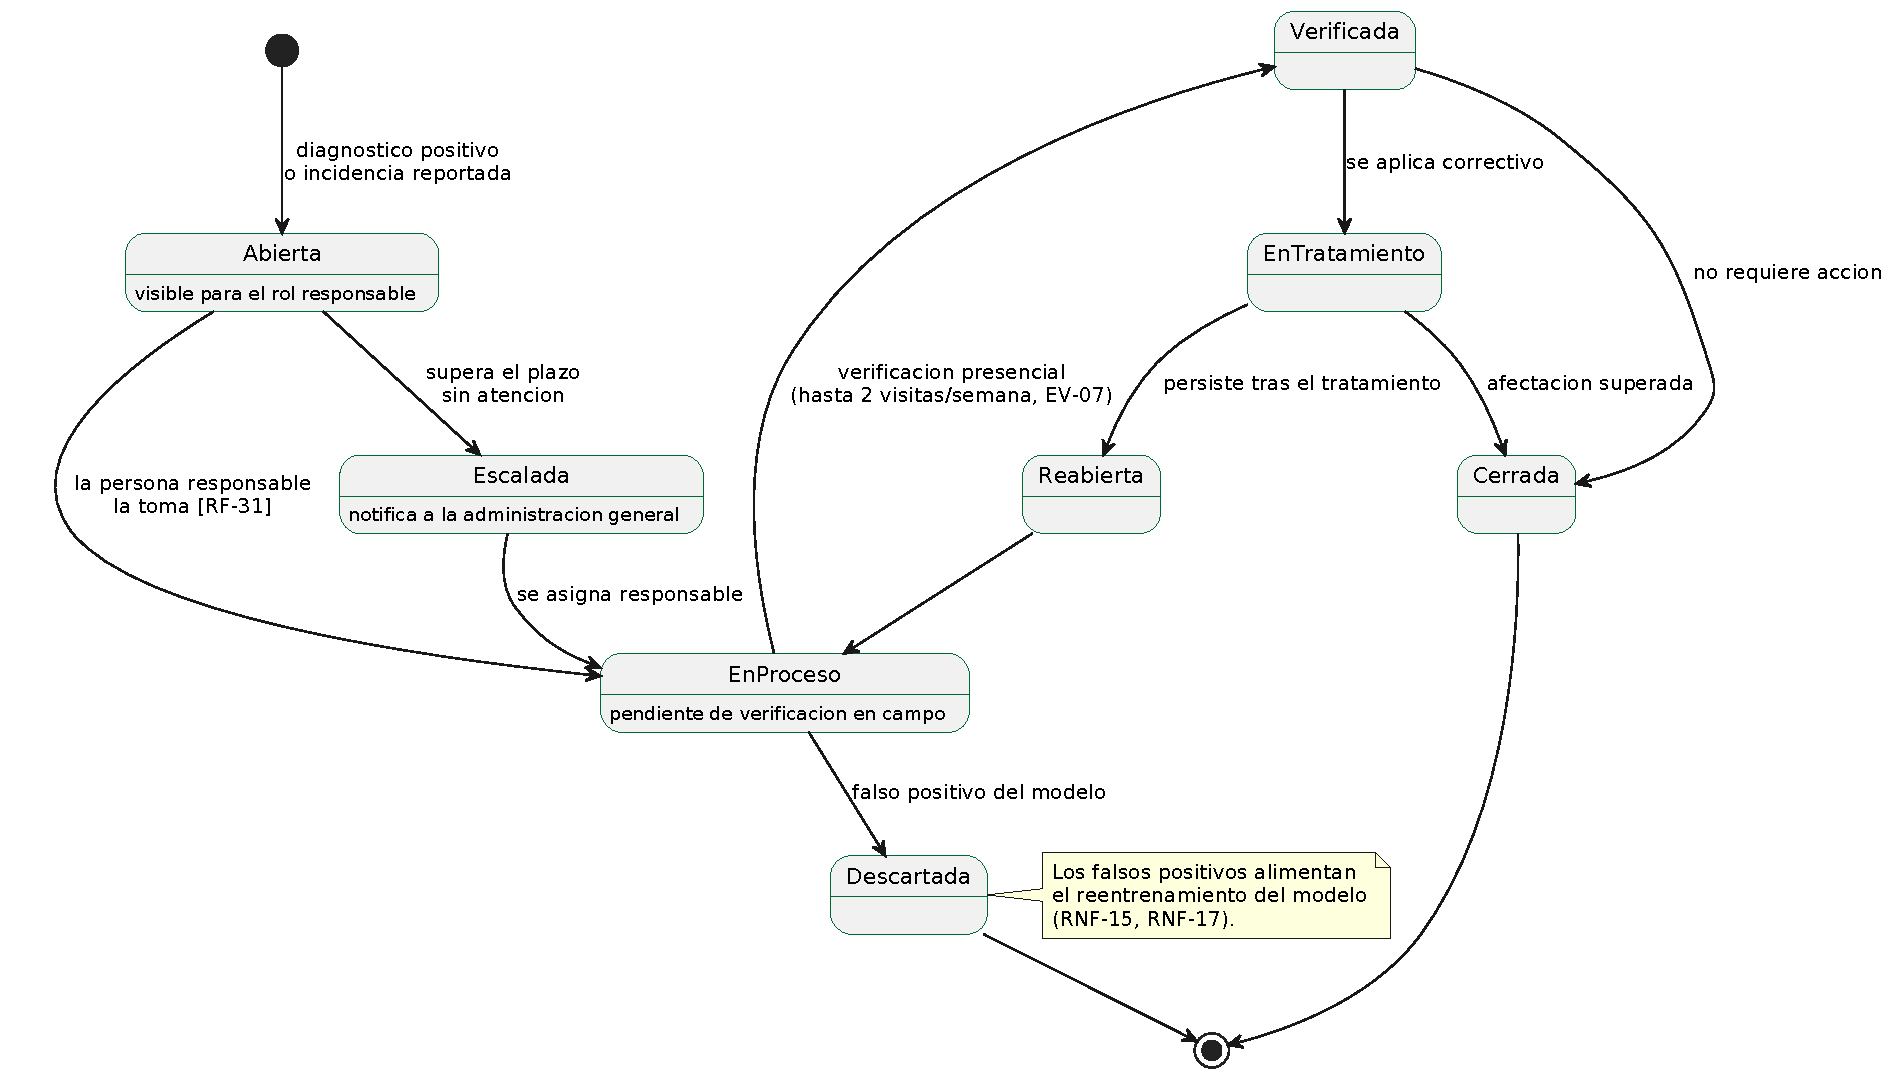
\includegraphics[width=1.0\textwidth]{img/estados_alerta}
\caption{Diagrama de estados de la alerta, con escalamiento por vencimiento de plazo y reapertura tras tratamiento inefectivo.}
\label{fig:est_alerta}
\end{figure}

\noindent
El estado \emph{Degradado} del racimo materializa el hallazgo de \id{EV-04} sobre la ventana entre
corte y entrega: el material híbrido tolera un intervalo mayor por su contenido de antioxidantes,
mientras que el \emph{guineensis} se deshidrata en dos o tres días. El estado \emph{Descartada} de
la alerta corresponde a los falsos positivos del modelo y alimenta el ciclo de reentrenamiento
previsto en \id{RNF-15} y \id{RNF-17}.

% ---------------------------------------------------------------------
\subsection{Diagrama de componentes}

\begin{figure}[!htbp]
\centering
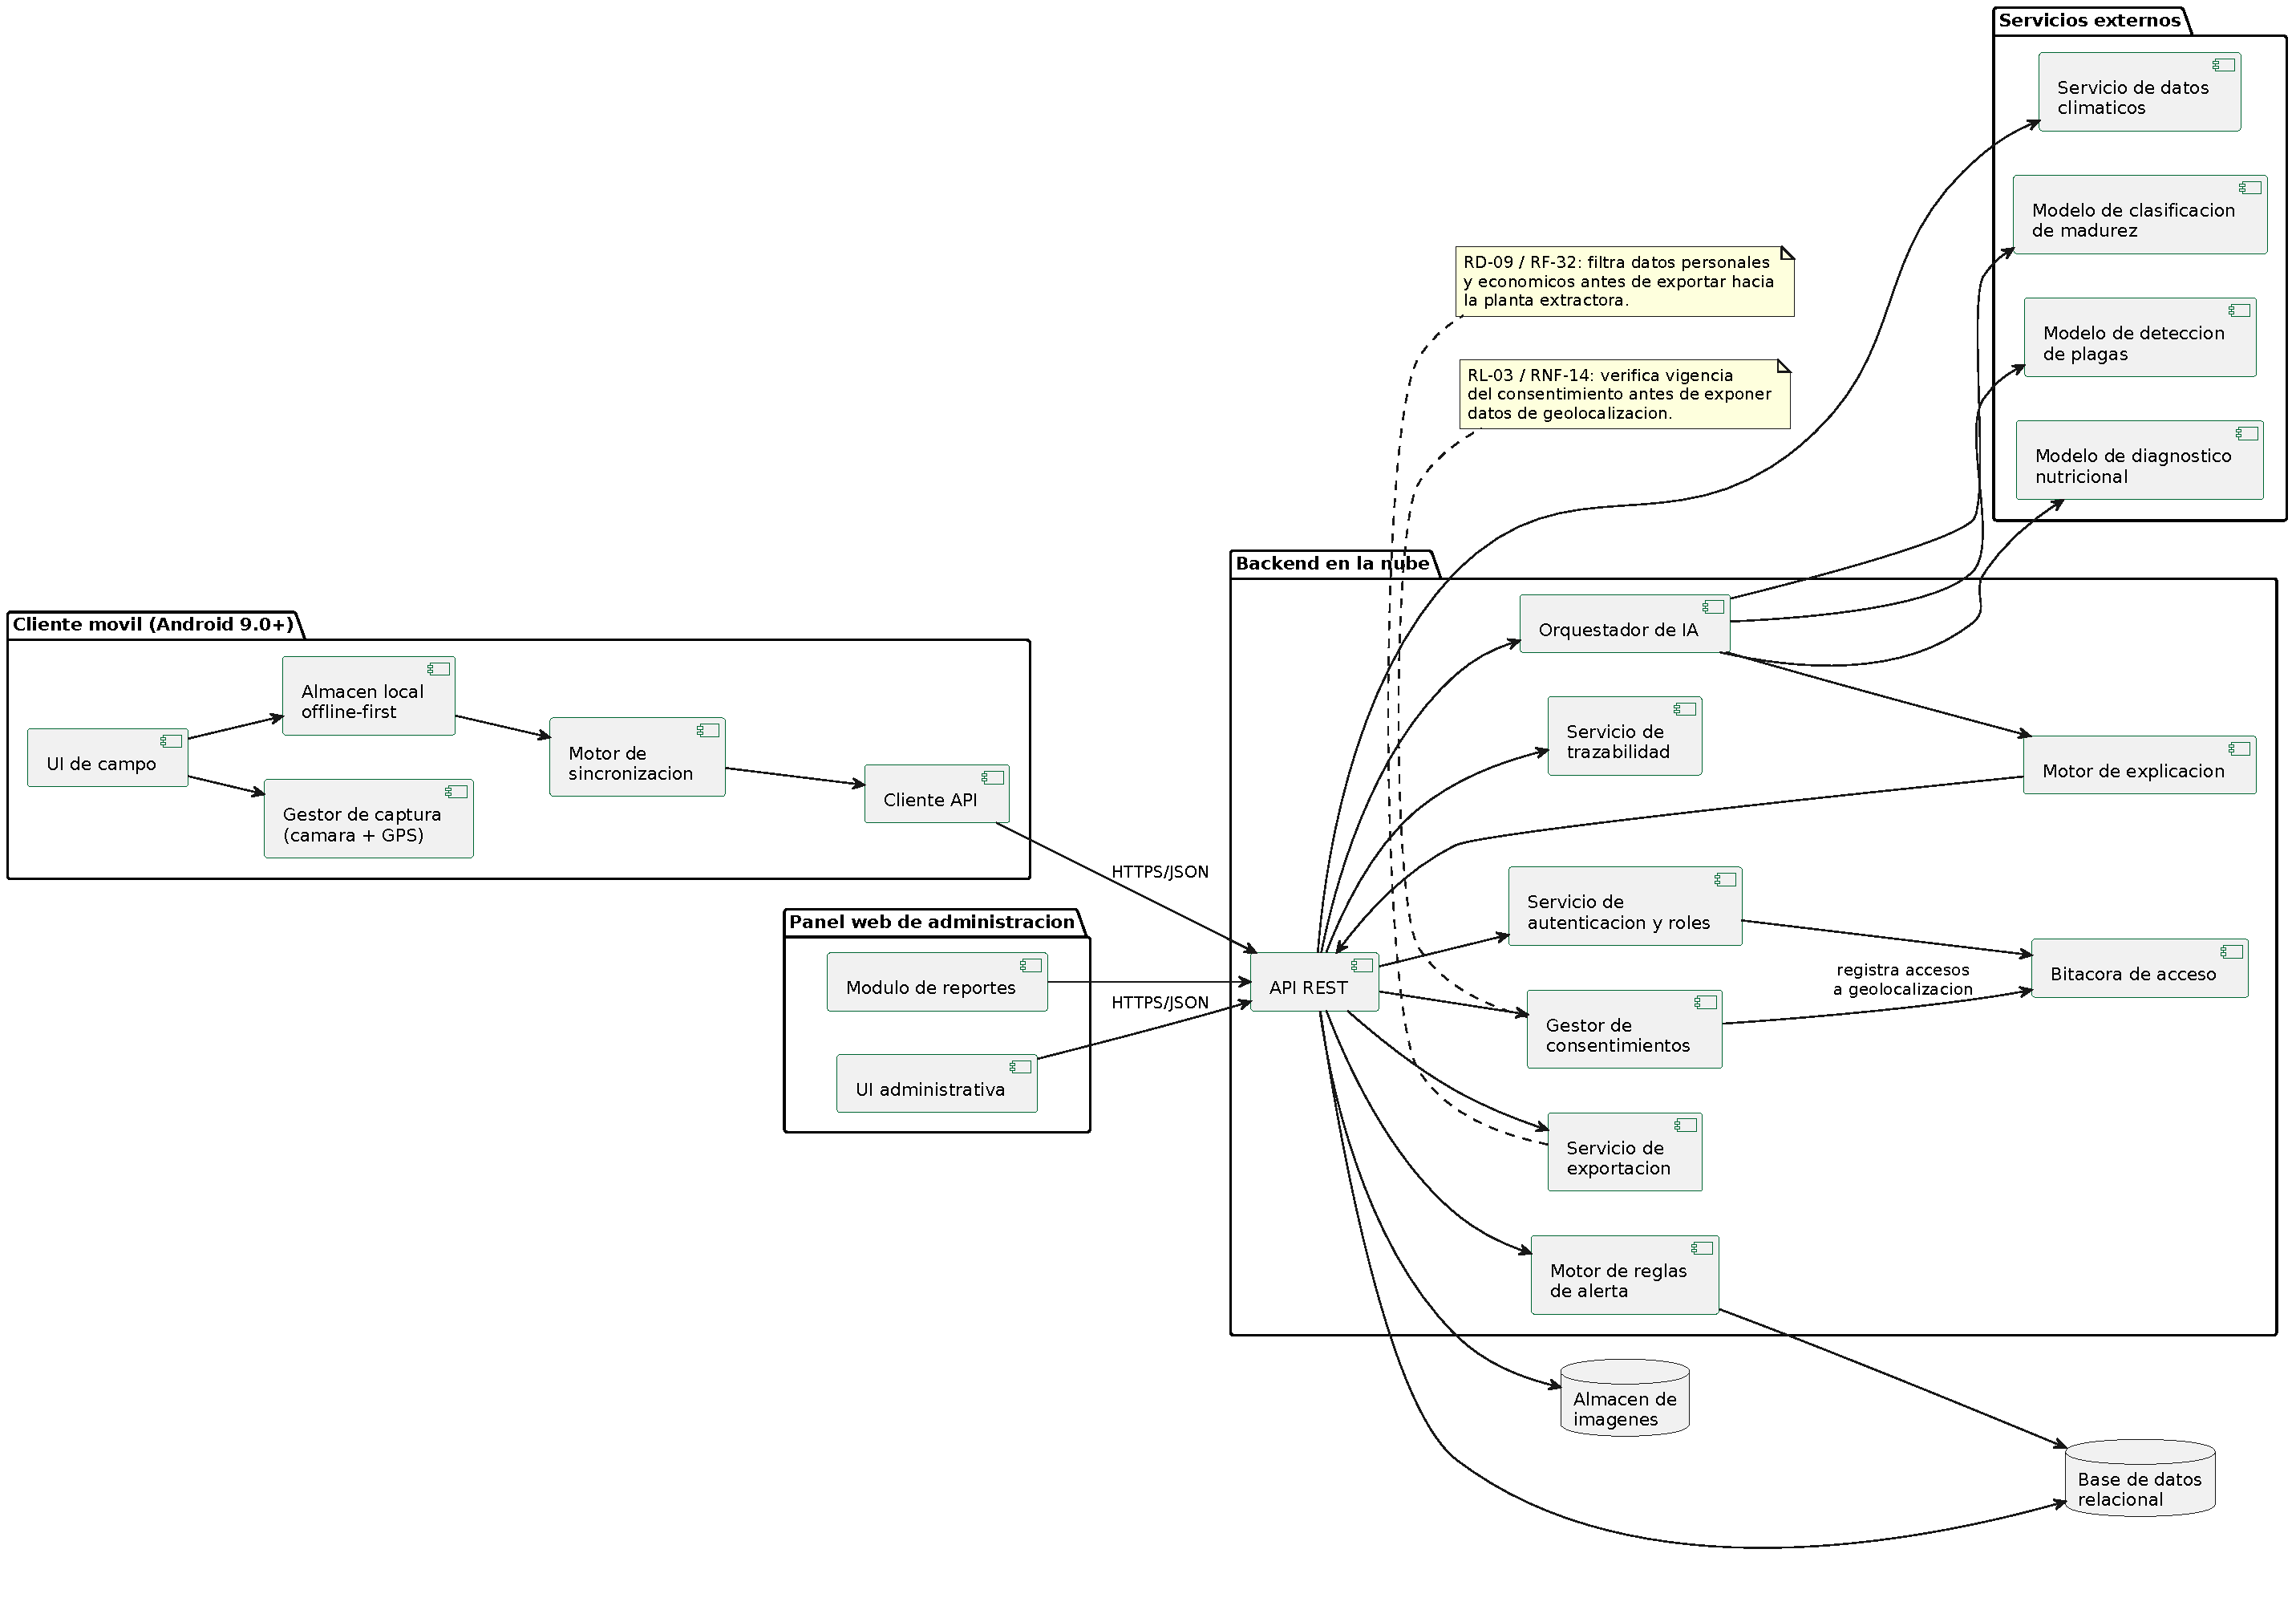
\includegraphics[width=1.0\textwidth]{img/componentes}
\caption{Diagrama de componentes del SIMPA.}
\label{fig:componentes}
\end{figure}

\noindent
Dos componentes merecen mención explícita por su origen normativo. El \emph{gestor de
consentimientos} verifica la vigencia antes de exponer cualquier dato de geolocalización y registra
todo acceso en la bitácora (\id{RL-03}, \id{RNF-14}). El \emph{servicio de exportación} filtra los
datos personales y económicos antes de generar el archivo destinado a la planta extractora
(\id{RD-09}, \id{RF-32}); su existencia como componente separado responde al criterio expreso de la
contraparte de que hay información que no puede compartirse (\id{EV-04}).

% ---------------------------------------------------------------------
\subsection{Diagrama de despliegue}

\begin{figure}[!htbp]
\centering
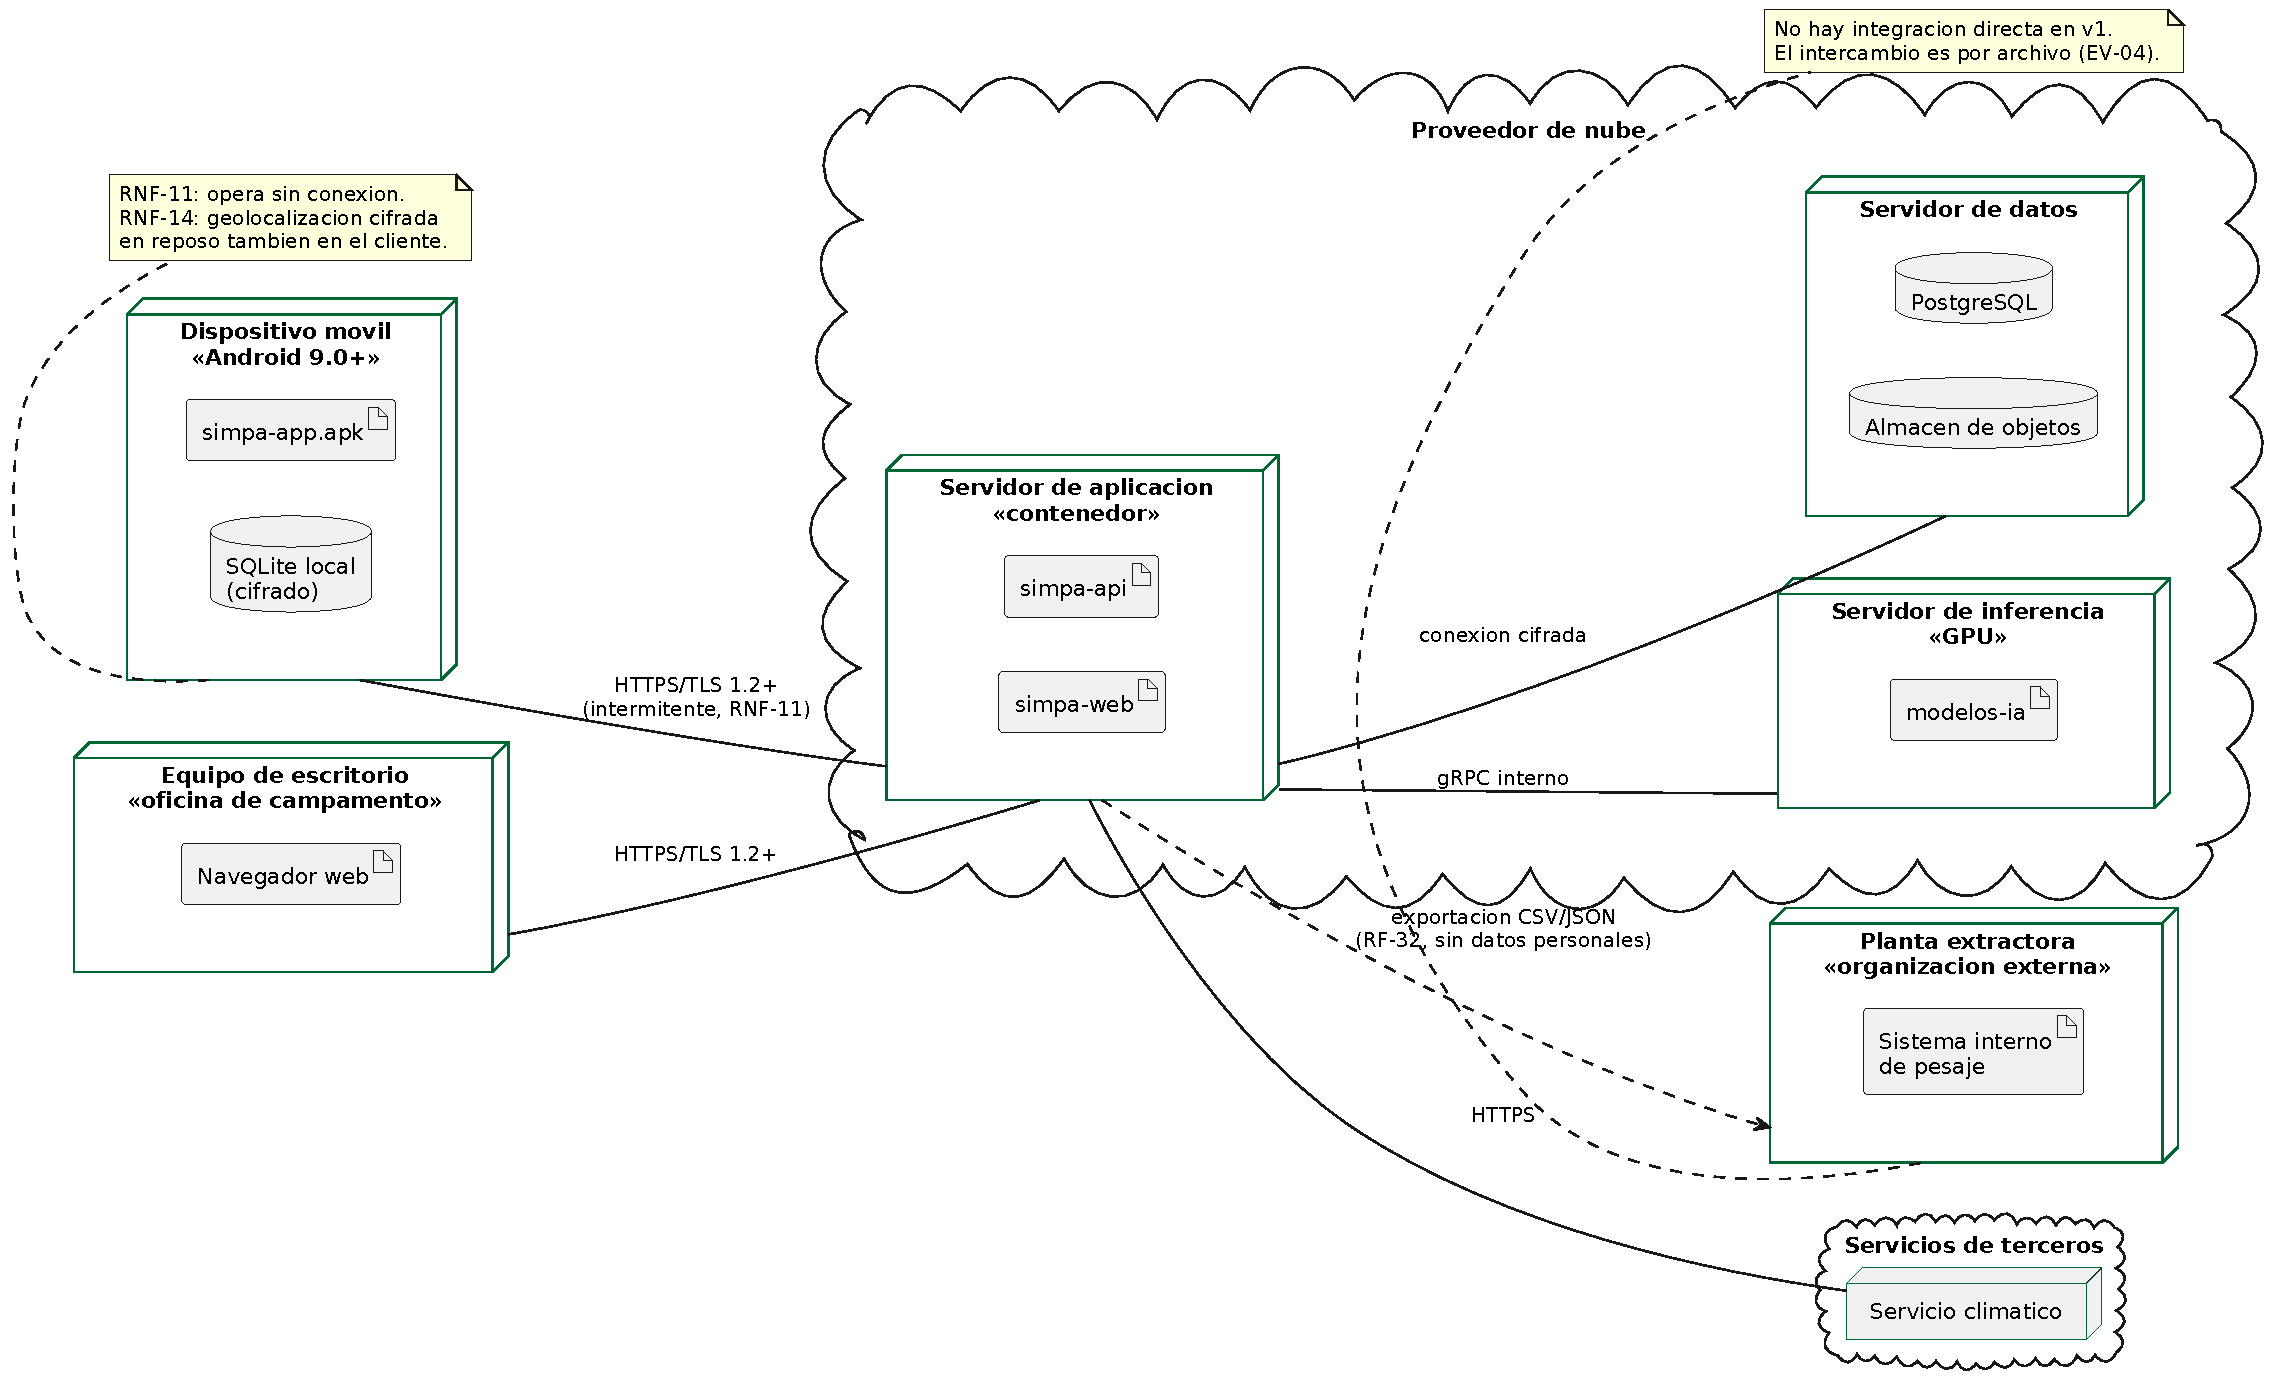
\includegraphics[width=1.0\textwidth]{img/despliegue}
\caption{Diagrama de despliegue del SIMPA.}
\label{fig:despliegue}
\end{figure}

\noindent
El enlace entre el dispositivo móvil y el servidor de aplicación se declara explícitamente como
\emph{intermitente}: el 74{,}2\% de las personas destinatarias no dispone de conectividad permanente
(\id{EV-12}). La planta extractora se representa como nodo externo sin integración directa; el
intercambio en la versión v1 se realiza por archivo, conforme a \id{RF-32}.

% ---------------------------------------------------------------------
\subsection{Cobertura del modelado}

\begin{longtable}{|L{4.6cm}|C{2.2cm}|C{2.2cm}|L{5.0cm}|}
\hline
\rowcolor{grisclaro}\textbf{Artefacto} & \textbf{Exigido} & \textbf{Entregado} & \textbf{Observación} \\
\hline
\endhead
Diagrama de casos de uso general & 1 & 1 & 8 actores, 18 casos de uso \\ \hline
Casos de uso detallados & 10 & 10 & Todos los \emph{Must}; $\geq 2$ flujos alternativos y $\geq 1$ excepción cada uno \\ \hline
Diagrama de clases refinado & 1 & 1 & 25 clases con atributos y operaciones \\ \hline
Diagramas de secuencia & CU \emph{Must} & 3 & CU-01, CU-03, CU-06 \\ \hline
Diagramas de actividad & Flujos principales & 1 & Ciclo semanal completo \\ \hline
Diagramas de estados & Entidades no triviales & 2 & Racimo y Alerta \\ \hline
Diagrama de componentes & 1 & 1 & --- \\ \hline
Diagrama de despliegue & 1 & 1 & --- \\ \hline
\caption{Cobertura del modelado UML frente a lo exigido en la §3.4 de la guía}
\end{longtable}

%  Requiere las imagenes en img/ generadas desde 03_Modelado/Diagramas_UML/
% =====================================================================

\newpage
\section{Modelado del sistema con UML}

El modelado emplea UML 2.5. Conforme a la §3.4 de la guía de la Entrega 3, se presentan ocho
diagramas: casos de uso general, especificación textual de diez casos de uso, clases refinado con
atributos y operaciones, tres diagramas de secuencia para los casos de uso \emph{Must}, actividad,
estados, componentes y despliegue. Todos se elaboraron en PlantUML y se entregan por triplicado
(fuente \id{.puml}, PNG a 300 dpi y SVG) en \id{03\_Modelado/Diagramas\_UML/}.

% ---------------------------------------------------------------------
\subsection{Diagrama general de casos de uso}

El diagrama presenta ocho actores y dieciocho casos de uso. Los actores primarios corresponden a los
seis perfiles de usuario de la §2.3; los actores secundarios son el servicio de análisis de IA y el
receptor GPS del dispositivo.

\begin{figure}[!htbp]
\centering
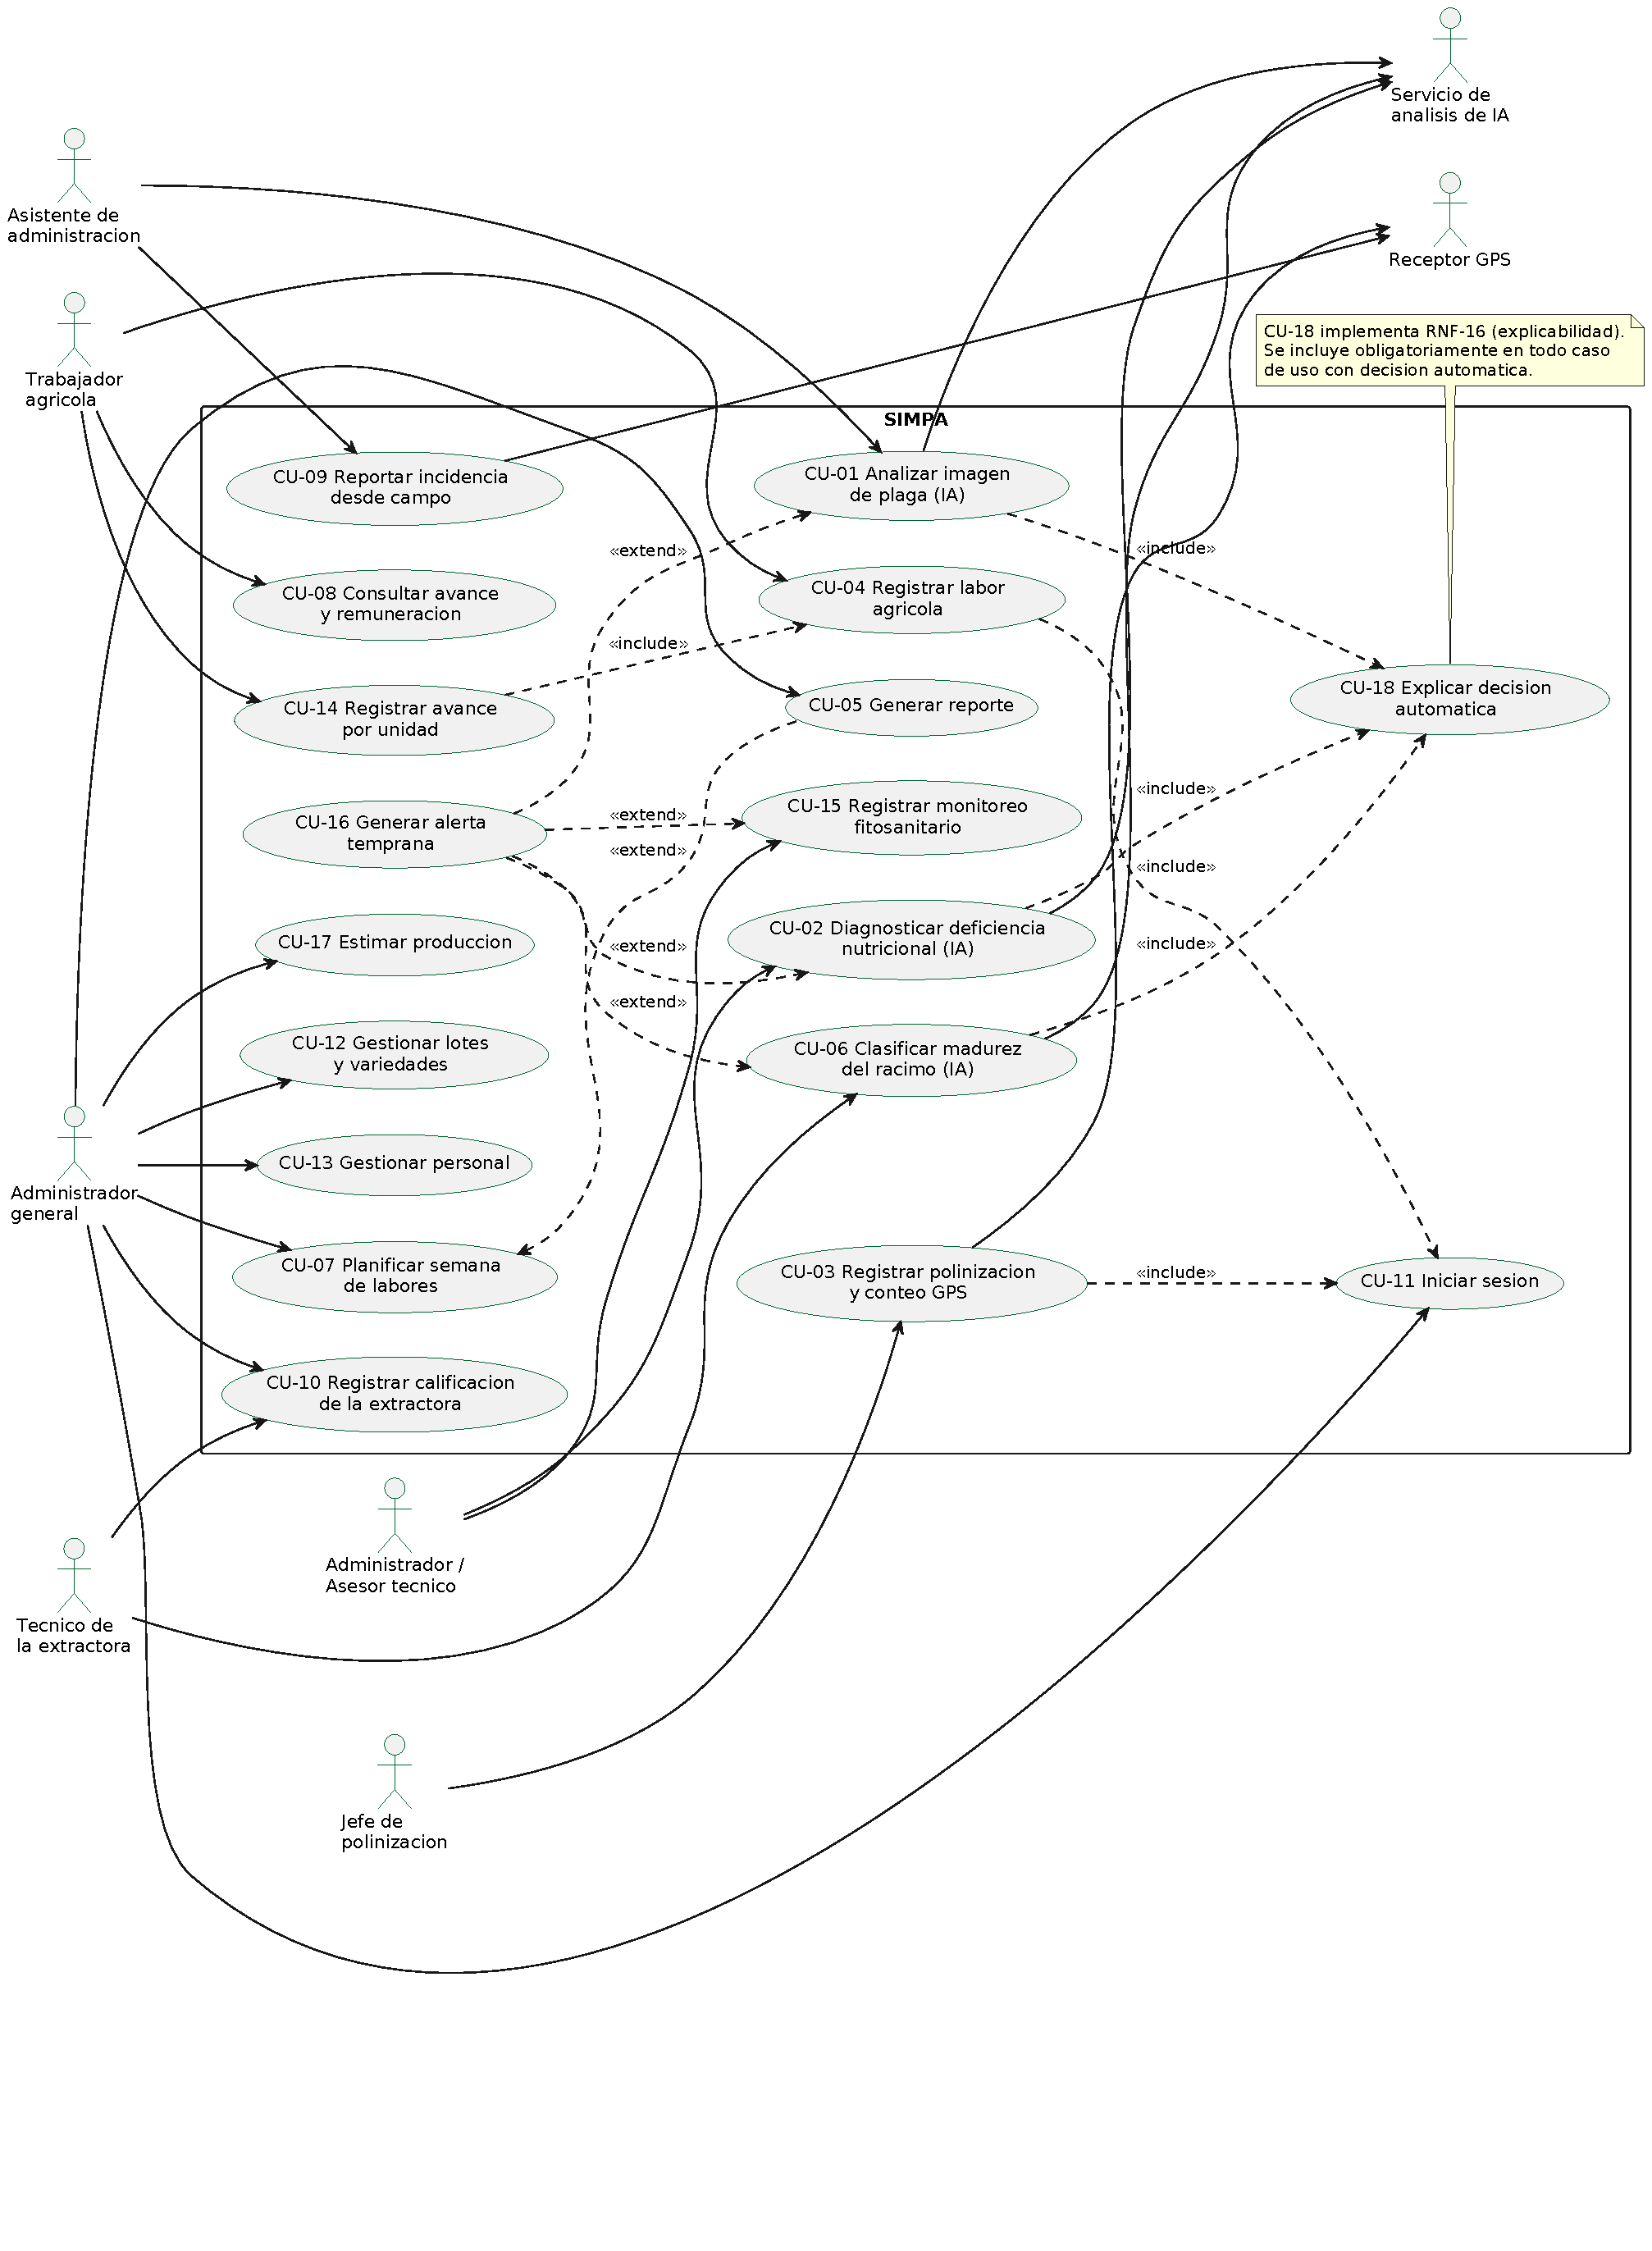
\includegraphics[width=0.91\textwidth]{img/casos_uso_general}
\caption{Diagrama general de casos de uso del SIMPA, con los ocho actores y el límite del sistema.}
\label{fig:cu_general}
\end{figure}

\noindent\textbf{Relaciones de inclusión y extensión.} \id{CU-14} incluye a \id{CU-04}, dado que el
registro de avance presupone una labor registrada. \id{CU-04} y \id{CU-03} incluyen a \id{CU-11},
por requerir sesión autenticada. Los tres casos de uso con decisión automática ---\id{CU-01},
\id{CU-02} y \id{CU-06}--- incluyen obligatoriamente a \id{CU-18}, que materializa el requisito de
explicabilidad \id{RNF-16}: no existe decisión automática sin explicación asociada. \id{CU-16}
extiende a los casos de diagnóstico y de monitoreo, puesto que la alerta se genera únicamente si el
resultado es positivo.

% ---------------------------------------------------------------------
\subsection{Especificación textual de los casos de uso}

Se especifican diez casos de uso, correspondientes a la totalidad de los requisitos funcionales de
prioridad \emph{Must}. Cada especificación incluye actores, precondiciones, postcondiciones, flujo
principal, al menos un flujo alternativo y al menos una excepción.

% --- CU-01
\begin{longtable}{|L{3.4cm}|L{12.0cm}|}
\hline
\rowcolor{grisclaro}\multicolumn{2}{|l|}{\textbf{CU-01 --- Analizar imagen para detectar plaga o enfermedad}}\\
\hline
\textbf{Requisitos} & \id{RF-07}, \id{RF-09}, \id{RF-12}, \id{RNF-16} \\ \hline
\textbf{Actores} & Primario: técnico fitosanitario / asistente de administración. Secundario: servicio de análisis de IA. \\ \hline
\textbf{Precondición} & Persona usuaria autenticada; lote seleccionado; cámara disponible. \\ \hline
\textbf{Postcondición} & El diagnóstico y su explicación quedan registrados y asociados al lote y a la fecha. \\ \hline
\textbf{Flujo principal} & 1. La persona usuaria selecciona el lote y la opción \emph{Analizar imagen}. \newline 2. Captura la fotografía de la palma o de la hoja. \newline 3. El sistema valida la calidad de la imagen. \newline 4. El sistema envía la imagen al servicio de IA con los parámetros de la variedad del lote. \newline 5. El servicio devuelve la clase de afectación, el nivel de confianza y el rasgo visual determinante. \newline 6. El sistema genera la explicación conforme a \id{RNF-16}. \newline 7. El sistema muestra el resultado, la explicación y la recomendación de control, y registra el diagnóstico. \\ \hline
\textbf{Flujo alternativo A} & \emph{Sin conectividad.} En el paso 4 el sistema almacena la imagen localmente y encola el análisis; al restablecerse la conexión lo ejecuta y notifica el resultado (\id{RNF-11}). \\ \hline
\textbf{Flujo alternativo B} & \emph{Confianza insuficiente.} Si el nivel de confianza es inferior al umbral configurado, el sistema no emite clasificación: informa que el resultado no es concluyente y sugiere repetir la captura o consultar a la asesoría técnica. \\ \hline
\textbf{Excepción E1} & Imagen de calidad insuficiente: el sistema solicita repetir la captura indicando el defecto detectado. \\ \hline
\textbf{Excepción E2} & Servicio de IA no disponible: el análisis queda en estado pendiente y la persona usuaria es notificada. \\ \hline
\textbf{Extensión} & Si el resultado es positivo, se ejecuta \id{CU-16} (generar alerta temprana). \\ \hline
\caption{CU-01 --- Analizar imagen para detectar plaga o enfermedad}
\end{longtable}

% --- CU-02
\begin{longtable}{|L{3.4cm}|L{12.0cm}|}
\hline
\rowcolor{grisclaro}\multicolumn{2}{|l|}{\textbf{CU-02 --- Diagnosticar deficiencia nutricional por imagen}}\\
\hline
\textbf{Requisitos} & \id{RF-08}, \id{RF-11}, \id{RNF-16} \\ \hline
\textbf{Actores} & Primario: administrador / asesor técnico. Secundario: servicio de análisis de IA. \\ \hline
\textbf{Precondición} & Persona usuaria autenticada; lote seleccionado con variedad asignada. \\ \hline
\textbf{Postcondición} & El diagnóstico nutricional y su recomendación quedan registrados en el historial del lote. \\ \hline
\textbf{Flujo principal} & 1. La persona usuaria selecciona \emph{Diagnóstico nutricional} y el lote. \newline 2. Captura la fotografía de la hoja. \newline 3. El sistema valida la imagen y la envía al servicio de IA. \newline 4. El servicio estima el elemento deficiente. \newline 5. El sistema genera una explicación de tipo causal, indicando qué signo foliar sustenta la estimación. \newline 6. El sistema muestra la deficiencia, la recomendación de fertilización y la explicación, y registra el diagnóstico. \\ \hline
\textbf{Flujo alternativo A} & La persona usuaria adjunta una imagen existente de la galería en lugar de capturarla. \\ \hline
\textbf{Flujo alternativo B} & \emph{Contraste con análisis de laboratorio.} Si el lote tiene un análisis de suelo o foliar registrado (\id{RF-11}), el sistema contrasta la estimación con los valores medidos y señala la discrepancia si la hubiere. \\ \hline
\textbf{Excepción E1} & Imagen no válida: el sistema solicita repetir la captura. \\ \hline
\textbf{Excepción E2} & Lote sin variedad asignada: el sistema advierte que la estimación puede no ser aplicable y solicita completar el dato. \\ \hline
\textbf{Extensión} & Si la deficiencia estimada es severa, se ejecuta \id{CU-16}. \\ \hline
\caption{CU-02 --- Diagnosticar deficiencia nutricional por imagen}
\end{longtable}

% --- CU-03
\begin{longtable}{|L{3.4cm}|L{12.0cm}|}
\hline
\rowcolor{grisclaro}\multicolumn{2}{|l|}{\textbf{CU-03 --- Registrar polinización y conteo georreferenciado}}\\
\hline
\textbf{Requisitos} & \id{RF-13}, \id{RF-14}, \id{RNF-05}, \id{RNF-12}, \id{RL-03} \\ \hline
\textbf{Actores} & Primario: polinizador. Secundario: receptor GPS. \\ \hline
\textbf{Precondición} & Lote en etapa de polinización; sesión iniciada; consentimiento de geolocalización vigente. \\ \hline
\textbf{Postcondición} & La polinización y el conteo diario quedan registrados por persona, lote y fecha, sin ingreso manual planta por planta. \\ \hline
\textbf{Flujo principal} & 1. El polinizador inicia la jornada en el lote. \newline 2. El sistema verifica la vigencia del consentimiento de geolocalización. \newline 3. El sistema activa el rastreo con período de muestreo de 30 s. \newline 4. Durante la jornada, el sistema almacena las marcaciones georreferenciadas. \newline 5. El polinizador registra el estado de la antesis y la verificación visual. \newline 6. Al cierre, el sistema calcula el número de flores polinizadas a partir de las marcaciones. \newline 7. El sistema almacena el registro y muestra el total a la persona trabajadora. \\ \hline
\textbf{Flujo alternativo A} & \emph{Consentimiento revocado.} Si el consentimiento no está vigente, el sistema no activa el rastreo y habilita el registro manual del número de flores, sin penalización para la persona trabajadora (\id{RL-03}). \\ \hline
\textbf{Flujo alternativo B} & \emph{Sin conectividad.} Las marcaciones se almacenan localmente y se sincronizan al reconectar (\id{RNF-11}). \\ \hline
\textbf{Excepción E1} & Precisión GPS superior a 10 m: el sistema conserva el dato marcándolo como de precisión degradada y advierte a la persona usuaria, sin descartar la jornada (\id{RNF-12}). \\ \hline
\textbf{Excepción E2} & Pérdida total de señal GPS durante la jornada: el sistema conserva el tramo registrado y solicita completar el conteo de forma manual para el tramo faltante. \\ \hline
\caption{CU-03 --- Registrar polinización y conteo georreferenciado}
\end{longtable}

% --- CU-04
\begin{longtable}{|L{3.4cm}|L{12.0cm}|}
\hline
\rowcolor{grisclaro}\multicolumn{2}{|l|}{\textbf{CU-04 --- Registrar labor agrícola}}\\
\hline
\textbf{Requisitos} & \id{RF-04}, \id{RF-28}, \id{RF-35} \\ \hline
\textbf{Actores} & Primario: trabajador agrícola. Alternativo: jefe de campo (registro delegado). \\ \hline
\textbf{Precondición} & Lote y persona trabajadora registrados; persona usuaria autenticada. \\ \hline
\textbf{Postcondición} & La labor y su avance quedan en el historial del lote y computan para el cumplimiento del plan semanal. \\ \hline
\textbf{Flujo principal} & 1. La persona usuaria selecciona el lote y el tipo de labor. \newline 2. Ingresa la cantidad ejecutada en la unidad correspondiente. \newline 3. El sistema valida que la unidad corresponda al tipo de labor. \newline 4. El sistema registra la labor asociada al lote, la fecha y la persona responsable. \newline 5. El sistema actualiza el avance acumulado del período y el cumplimiento de la meta semanal. \\ \hline
\textbf{Flujo alternativo A} & \emph{Registro delegado.} Si la persona trabajadora no dispone de dispositivo propio, el jefe de campo registra el avance en su nombre; el sistema conserva en bitácora la identidad de quien efectuó el registro (\id{RF-35}, \id{RD-10}). \\ \hline
\textbf{Flujo alternativo B} & \emph{Sin conectividad.} La labor se almacena localmente y se sincroniza al reconectar. \\ \hline
\textbf{Excepción E1} & Datos incompletos: el sistema impide guardar y señala los campos faltantes. \\ \hline
\textbf{Excepción E2} & Unidad incompatible con el tipo de labor: el sistema rechaza el registro e indica la unidad esperada. \\ \hline
\caption{CU-04 --- Registrar labor agrícola}
\end{longtable}

% --- CU-05
\begin{longtable}{|L{3.4cm}|L{12.0cm}|}
\hline
\rowcolor{grisclaro}\multicolumn{2}{|l|}{\textbf{CU-05 --- Generar reporte}}\\
\hline
\textbf{Requisitos} & \id{RF-19}, \id{RF-26} \\ \hline
\textbf{Actores} & Primario: administrador general. \\ \hline
\textbf{Precondición} & Existen registros en el período seleccionado. \\ \hline
\textbf{Postcondición} & El reporte queda disponible para consulta o exportación. \\ \hline
\textbf{Flujo principal} & 1. La persona administradora selecciona el tipo de reporte y el período. \newline 2. El sistema consolida labores, avance, producción y alertas del período. \newline 3. El sistema genera y presenta el reporte. \newline 4. La persona administradora lo consulta o lo exporta a PDF o a hoja de cálculo. \\ \hline
\textbf{Flujo alternativo A} & Filtrado por lote, por equipo o por persona trabajadora. \\ \hline
\textbf{Flujo alternativo B} & \emph{Reporte de cumplimiento semanal.} El sistema contrasta el plan de la semana con lo ejecutado y destaca las metas no alcanzadas y su remanente. \\ \hline
\textbf{Excepción E1} & Sin registros en el período: el sistema informa la ausencia de datos y propone un período alternativo con información disponible. \\ \hline
\caption{CU-05 --- Generar reporte}
\end{longtable}

% --- CU-06
\begin{longtable}{|L{3.4cm}|L{12.0cm}|}
\hline
\rowcolor{grisclaro}\multicolumn{2}{|l|}{\textbf{CU-06 --- Clasificar la madurez del racimo}}\\
\hline
\textbf{Requisitos} & \id{RF-21}, \id{RF-22}, \id{RD-07}, \id{RD-08}, \id{RNF-01}, \id{RNF-16} \\ \hline
\textbf{Actores} & Primario: cosechador / técnico de la extractora. Secundario: servicio de análisis de IA. \\ \hline
\textbf{Precondición} & Lote con variedad asignada; persona usuaria autenticada. \\ \hline
\textbf{Postcondición} & La clasificación queda asociada al racimo, al lote y a la fecha, y actualiza el porcentaje estimado de fruta verde del lote. \\ \hline
\textbf{Flujo principal} & 1. La persona usuaria selecciona el lote y la opción \emph{Clasificar racimo}. \newline 2. El sistema recupera el umbral de desprendimiento de la variedad del lote. \newline 3. La persona usuaria captura la fotografía de la parte basal del racimo. \newline 4. El servicio de IA cuenta los frutos desprendidos, sin emplear el color como criterio (\id{RD-07}). \newline 5. El sistema compara el conteo con el umbral de la variedad y determina el estado. \newline 6. El sistema genera una explicación por contraste, indicando el conteo obtenido y el umbral aplicable. \newline 7. El sistema registra la clasificación y actualiza el porcentaje de fruta verde del lote. \\ \hline
\textbf{Flujo alternativo A} & \emph{Verificación previa al despacho.} La persona usuaria solicita el porcentaje estimado de fruta verde del lote; si alcanza o supera el umbral de penalización, el sistema emite alerta preventiva y desaconseja el despacho (\id{RF-22}). \\ \hline
\textbf{Flujo alternativo B} & \emph{Sobremadurez.} Si el conteo excede ampliamente el umbral, el sistema clasifica el racimo como sobremaduro y advierte sobre el incremento de acidez. \\ \hline
\textbf{Excepción E1} & Lote sin variedad asignada: el sistema no clasifica y solicita completar el dato, dado que el umbral depende de la variedad. \\ \hline
\textbf{Excepción E2} & Parte basal no visible en la imagen: el sistema solicita repetir la captura indicando el encuadre requerido. \\ \hline
\caption{CU-06 --- Clasificar la madurez del racimo}
\end{longtable}

% --- CU-07
\begin{longtable}{|L{3.4cm}|L{12.0cm}|}
\hline
\rowcolor{grisclaro}\multicolumn{2}{|l|}{\textbf{CU-07 --- Planificar la semana de labores}}\\
\hline
\textbf{Requisitos} & \id{RF-26}, \id{RF-27}, \id{RF-34}, \id{RF-37} a \id{RF-39} \\ \hline
\textbf{Actores} & Primario: administrador general. \\ \hline
\textbf{Precondición} & Lotes y tipos de labor registrados. \\ \hline
\textbf{Postcondición} & El plan de la semana queda publicado y disponible para el seguimiento diario. \\ \hline
\textbf{Flujo principal} & 1. La persona administradora crea el plan de la semana. \newline 2. Para cada lote, define las labores previstas con su meta y unidad. \newline 3. El sistema incorpora automáticamente los remanentes arrastrados de la semana anterior. \newline 4. La persona administradora registra los insumos requeridos. \newline 5. El sistema publica el plan y lo hace visible al jefe de campo. \\ \hline
\textbf{Flujo alternativo A} & \emph{Cierre de semana.} Al cierre, el sistema calcula el cumplimiento de cada meta; si es parcial, genera el remanente como labor pendiente de la semana siguiente, vinculada a la de origen (\id{RF-27}). \\ \hline
\textbf{Flujo alternativo B} & Ajuste del plan durante la semana en curso, conservando la versión previa en bitácora. \\ \hline
\textbf{Flujo alternativo C} & \emph{Liquidación y aprobación.} Al cierre, el sistema genera la liquidación que contrasta cantidad presupuestada, cantidad ejecutada, tarifa y valor por grupo de labor, totaliza el gasto presupuestado frente al real, e incorpora las labores no presupuestadas en su grupo diferenciado (\id{RF-37}, \id{RF-38}). La persona administradora aprueba la liquidación y el período queda cerrado (\id{RF-39}). \\ \hline
\textbf{Excepción E1} & Meta expresada en unidad incompatible con el tipo de labor: el sistema rechaza la meta e indica la unidad esperada. \\ \hline
\textbf{Excepción E2} & Existe un plan publicado para la misma semana: el sistema advierte y solicita confirmación antes de sustituirlo. \\ \hline
\caption{CU-07 --- Planificar la semana de labores}
\end{longtable}

% --- CU-08
\begin{longtable}{|L{3.4cm}|L{12.0cm}|}
\hline
\rowcolor{grisclaro}\multicolumn{2}{|l|}{\textbf{CU-08 --- Consultar avance acumulado y remuneración estimada}}\\
\hline
\textbf{Requisitos} & \id{RF-29}, \id{RF-36}, \id{RL-04} \\ \hline
\textbf{Actores} & Primario: trabajador agrícola. \\ \hline
\textbf{Precondición} & Existen registros de avance de la persona trabajadora en el período. \\ \hline
\textbf{Postcondición} & Se presenta el consolidado del período, sin posibilidad de edición por parte de la persona trabajadora. \\ \hline
\textbf{Flujo principal} & 1. La persona trabajadora accede a \emph{Mi avance}. \newline 2. Selecciona el período (quincena en curso por defecto). \newline 3. El sistema agrega sus registros de avance por tipo de labor. \newline 4. El sistema obtiene del catálogo la tarifa vigente de cada tipo de labor a la fecha de cada registro y calcula la remuneración estimada correspondiente al trabajo por avance. \newline 5. El sistema presenta el desglose por labor y el total estimado. \\ \hline
\textbf{Flujo alternativo A} & \emph{Ejercicio del derecho de acceso.} La persona trabajadora solicita la exportación de sus datos personales; el sistema genera el archivo conforme al Art. 12 de la LOPDP (\id{RL-04}). \\ \hline
\textbf{Flujo alternativo B} & \emph{Discrepancia.} La persona trabajadora marca un registro como discrepante; el sistema notifica a la administración sin modificar el dato original, y la corrección se tramita mediante \id{RL-05}. \\ \hline
\textbf{Excepción E1} & Sin registros en el período: el sistema informa la ausencia de datos. \\ \hline
\textbf{Excepción E2} & La labor carece de tarifa vigente en el catálogo (\id{RF-36}) a la fecha del registro: el sistema muestra el avance en unidades, omite la estimación monetaria e indica que la tarifa no está vigente para esa fecha. \\ \hline
\caption{CU-08 --- Consultar avance acumulado y remuneración estimada}
\end{longtable}

% --- CU-09
\begin{longtable}{|L{3.4cm}|L{12.0cm}|}
\hline
\rowcolor{grisclaro}\multicolumn{2}{|l|}{\textbf{CU-09 --- Reportar incidencia desde el campo}}\\
\hline
\textbf{Requisitos} & \id{RF-30}, \id{RF-31}, \id{RF-12} \\ \hline
\textbf{Actores} & Primario: asistente de administración / trabajador agrícola. Secundario: receptor GPS. \\ \hline
\textbf{Precondición} & Persona usuaria autenticada; cámara y GPS disponibles. \\ \hline
\textbf{Postcondición} & La incidencia queda registrada con fotografía y coordenadas, e incorporada a la lista de pendientes de verificación. \\ \hline
\textbf{Flujo principal} & 1. La persona usuaria selecciona \emph{Reportar incidencia}. \newline 2. Captura la fotografía de la afectación. \newline 3. El sistema obtiene las coordenadas del punto. \newline 4. La persona usuaria selecciona el lote y describe la afectación. \newline 5. El sistema registra la incidencia georreferenciada. \newline 6. El sistema la incorpora a la lista de pendientes de la persona supervisora. \\ \hline
\textbf{Flujo alternativo A} & \emph{Análisis asistido.} La persona usuaria solicita el análisis de la fotografía; se ejecuta \id{CU-01} y el diagnóstico se asocia a la incidencia. \\ \hline
\textbf{Flujo alternativo B} & \emph{Verificación en visita.} La persona supervisora recorre su lista de pendientes, ubica la incidencia por sus coordenadas y la marca como verificada o descartada. \\ \hline
\textbf{Excepción E1} & GPS no disponible: el sistema registra la incidencia solicitando la selección manual del lote y la marca como de ubicación aproximada. \\ \hline
\textbf{Excepción E2} & Sin conectividad: la incidencia se encola y se sincroniza al reconectar, conservando el instante original de captura. \\ \hline
\caption{CU-09 --- Reportar incidencia desde el campo}
\end{longtable}

% --- CU-10
\begin{longtable}{|L{3.4cm}|L{12.0cm}|}
\hline
\rowcolor{grisclaro}\multicolumn{2}{|l|}{\textbf{CU-10 --- Registrar la calificación de la planta extractora}}\\
\hline
\textbf{Requisitos} & \id{RF-23}, \id{RF-24}, \id{RF-25}, \id{RF-33} \\ \hline
\textbf{Actores} & Primario: administrador general. \\ \hline
\textbf{Precondición} & Existe un despacho registrado con su fecha de corte. \\ \hline
\textbf{Postcondición} & La calificación queda asociada al lote de origen y disponible para el análisis de trazabilidad. \\ \hline
\textbf{Flujo principal} & 1. La persona administradora selecciona el despacho. \newline 2. Ingresa los datos del ticket de pesaje: peso bruto, tara y neto. \newline 3. Ingresa la calificación de calidad: tamaño del fruto, porcentaje de fruta verde, sobremadura, malformación y pedúnculo largo. \newline 4. El sistema calcula el intervalo entre el corte y la entrega. \newline 5. El sistema registra la calificación y la asocia al lote de origen. \\ \hline
\textbf{Flujo alternativo A} & \emph{Análisis de trazabilidad.} Ante una calificación desfavorable, la persona administradora consulta la cadena lote $\rightarrow$ fecha de corte $\rightarrow$ cuadrilla, y contrasta con las labores del período para distinguir si el origen está en la cosecha o en el manejo del cultivo (\id{RF-24}). \\ \hline
\textbf{Flujo alternativo B} & \emph{Ausencia de guía de remisión.} Si el despacho se registra sin número de guía, el sistema advierte antes del cierre (\id{RF-33}). \\ \hline
\textbf{Excepción E1} & El intervalo entre corte y entrega supera el valor recomendado para la variedad: el sistema registra la advertencia junto al despacho (\id{RF-25}). \\ \hline
\textbf{Excepción E2} & La suma de pesos es inconsistente (neto distinto de bruto menos tara): el sistema rechaza el registro e indica la inconsistencia. \\ \hline
\caption{CU-10 --- Registrar la calificación de la planta extractora}
\end{longtable}

% ---------------------------------------------------------------------
\subsection{Diagrama de clases refinado}

El modelo del dominio comprende veinticinco clases con atributos y operaciones. Incorpora tres
jerarquías de herencia (\id{Persona}--\id{Usuario} y la especialización de \id{Diagnostico} en sus
tres variantes), cuatro relaciones de composición y asociaciones con multiplicidad explícita. No
corresponde a un diseño de base de datos, sino al modelo conceptual del dominio del problema.

\begin{figure}[!htbp]
\centering
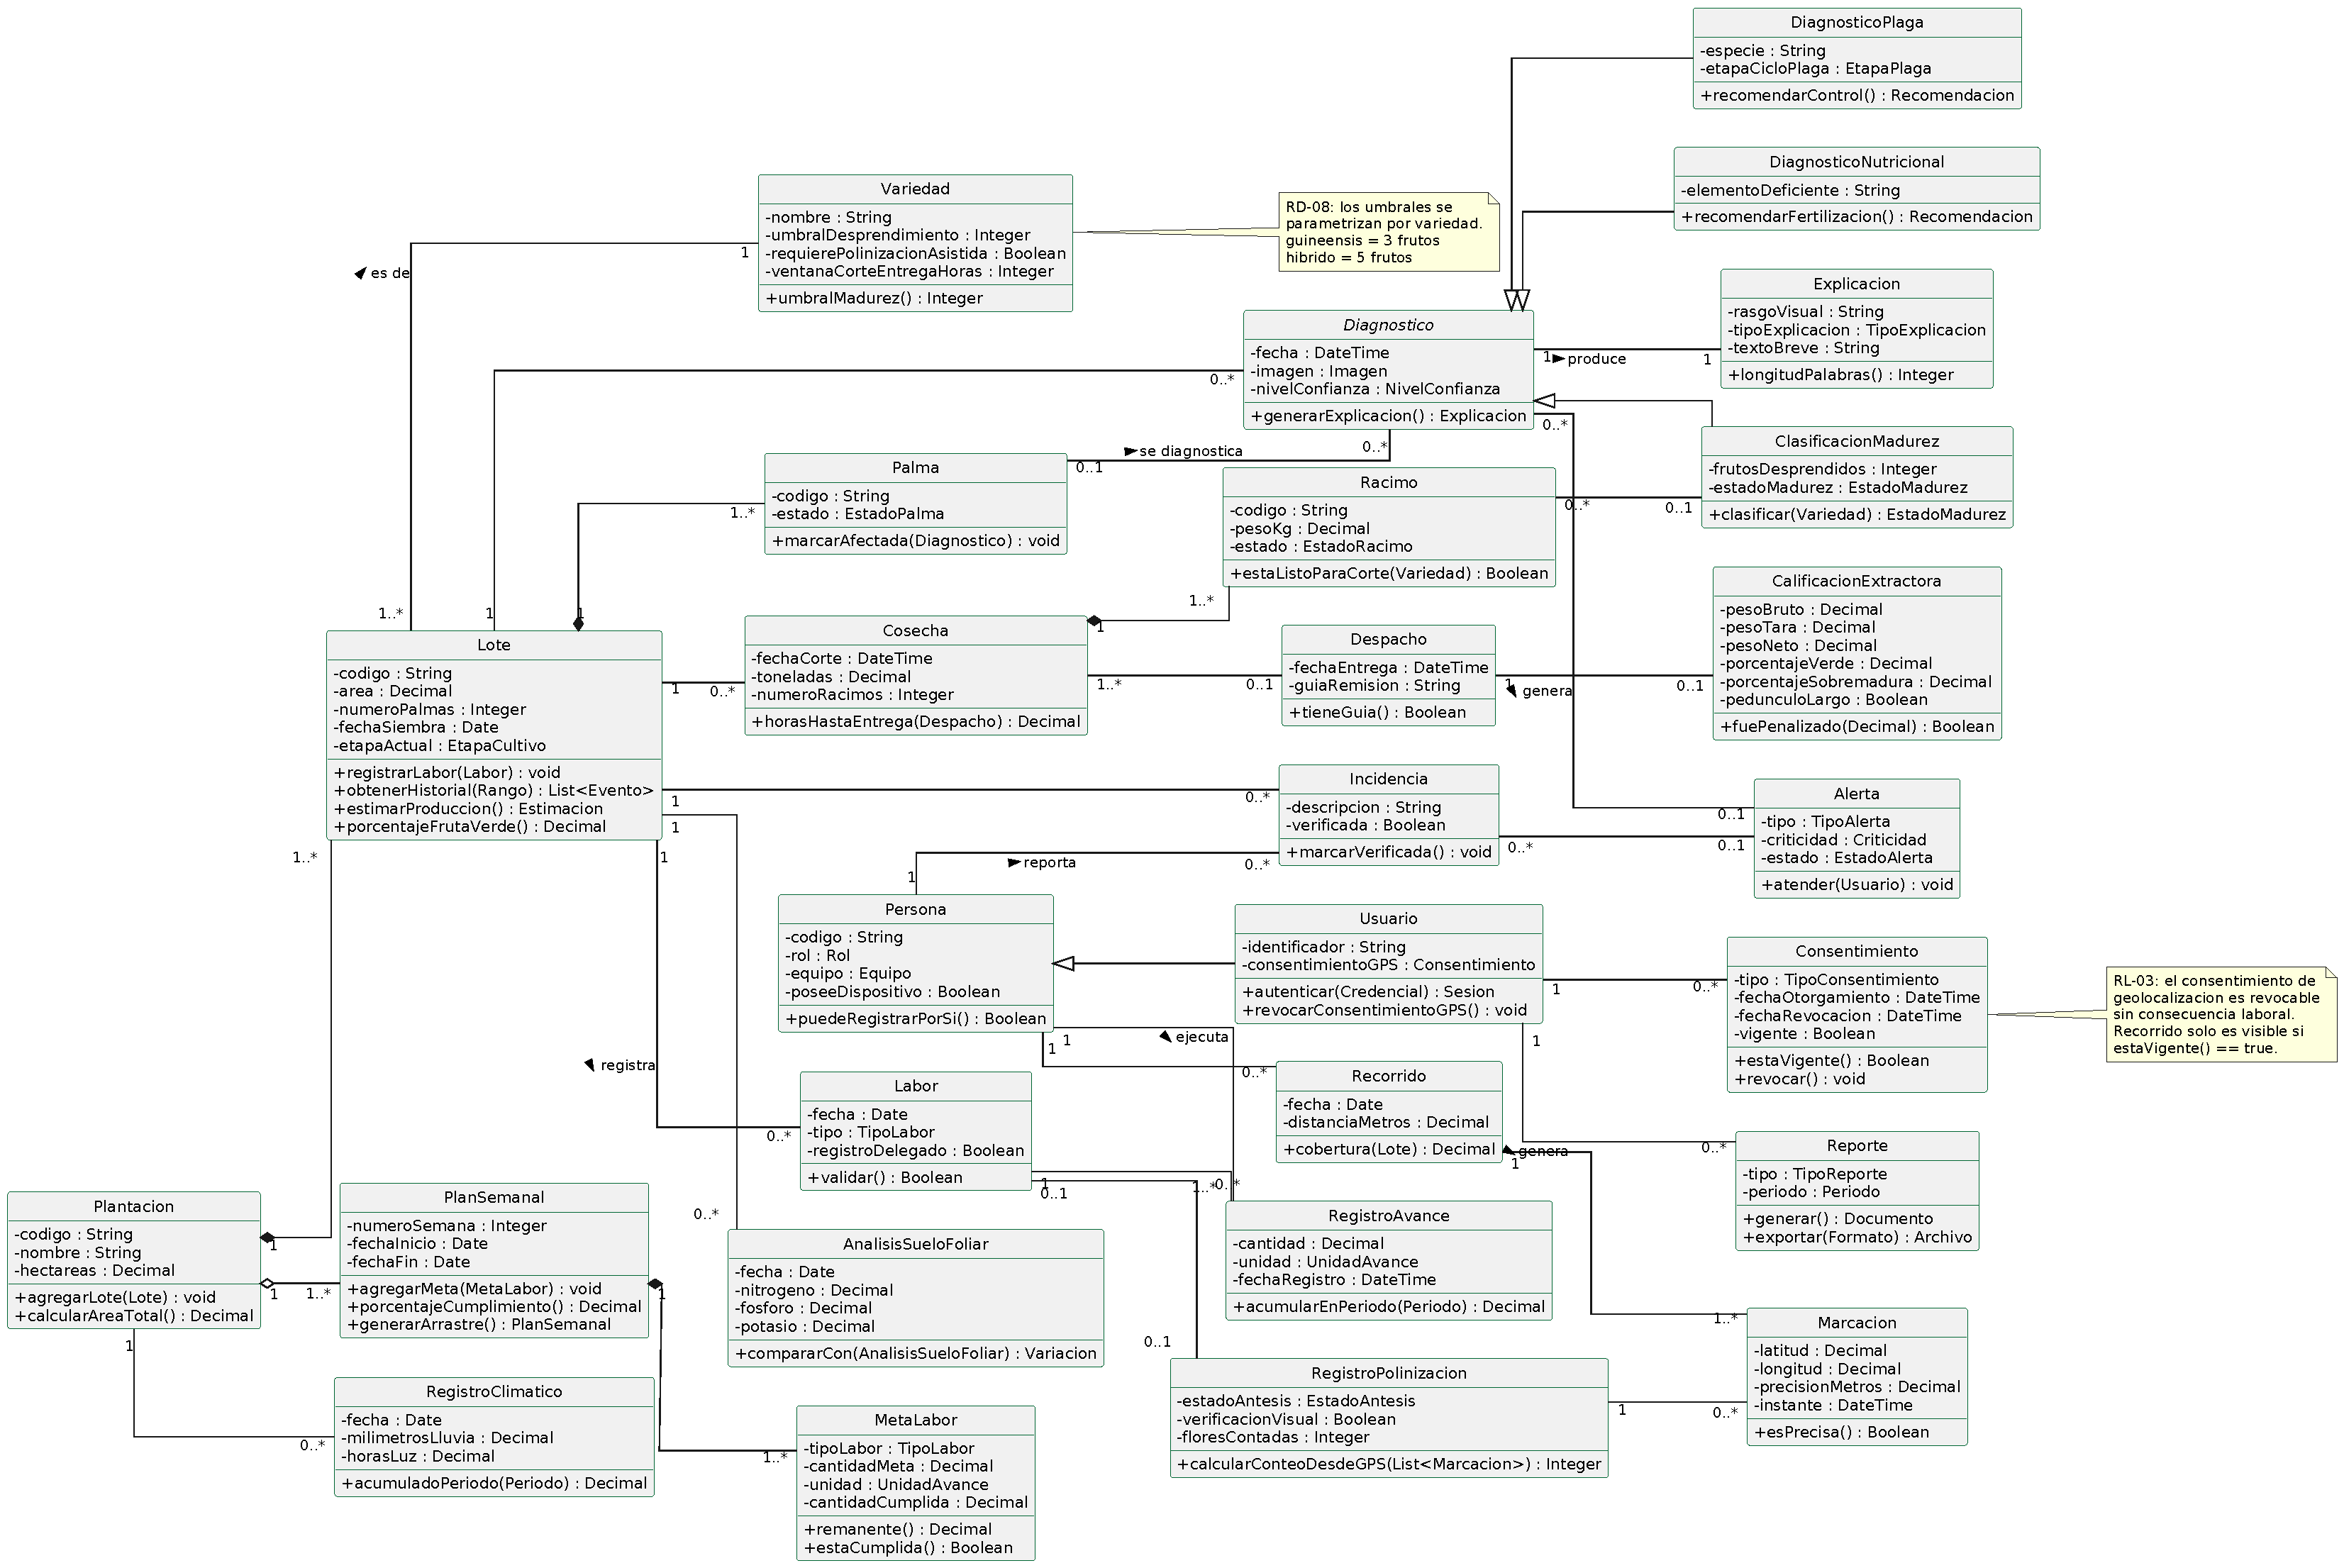
\includegraphics[width=1.0\textwidth]{img/clases_refinado}
\caption{Diagrama de clases refinado del SIMPA, con atributos y operaciones.}
\label{fig:clases}
\end{figure}

\noindent\textbf{Decisiones de modelado relevantes.} La clase \id{Consentimiento} se modela como
entidad de primer orden y no como atributo booleano de \id{Usuario}, porque el Art. 7 de la LOPDP
exige que el consentimiento sea específico por finalidad y revocable, lo que obliga a conservar su
historia. La clase \id{Variedad} concentra los umbrales de decisión ---desprendimiento, ventana
corte-entrega y necesidad de polinización asistida--- en lugar de fijarlos en la lógica de los
módulos de IA, conforme a \id{RD-08}. La clase \id{Explicacion} se asocia de forma obligatoria a
\id{Diagnostico} con multiplicidad 1:1, de modo que el modelo impide estructuralmente la existencia
de una decisión automática sin explicación (\id{RNF-16}). La clase \id{RegistroAvance} se separa de
\id{Labor} porque una labor puede acumular avances de varias personas y días, patrón observado en
los documentos de planificación semanal (\id{EV-11}).

% ---------------------------------------------------------------------
\subsection{Diagramas de secuencia}

Se presentan los diagramas de secuencia de los tres casos de uso \emph{Must} de mayor complejidad
de interacción.

\begin{figure}[!htbp]
\centering
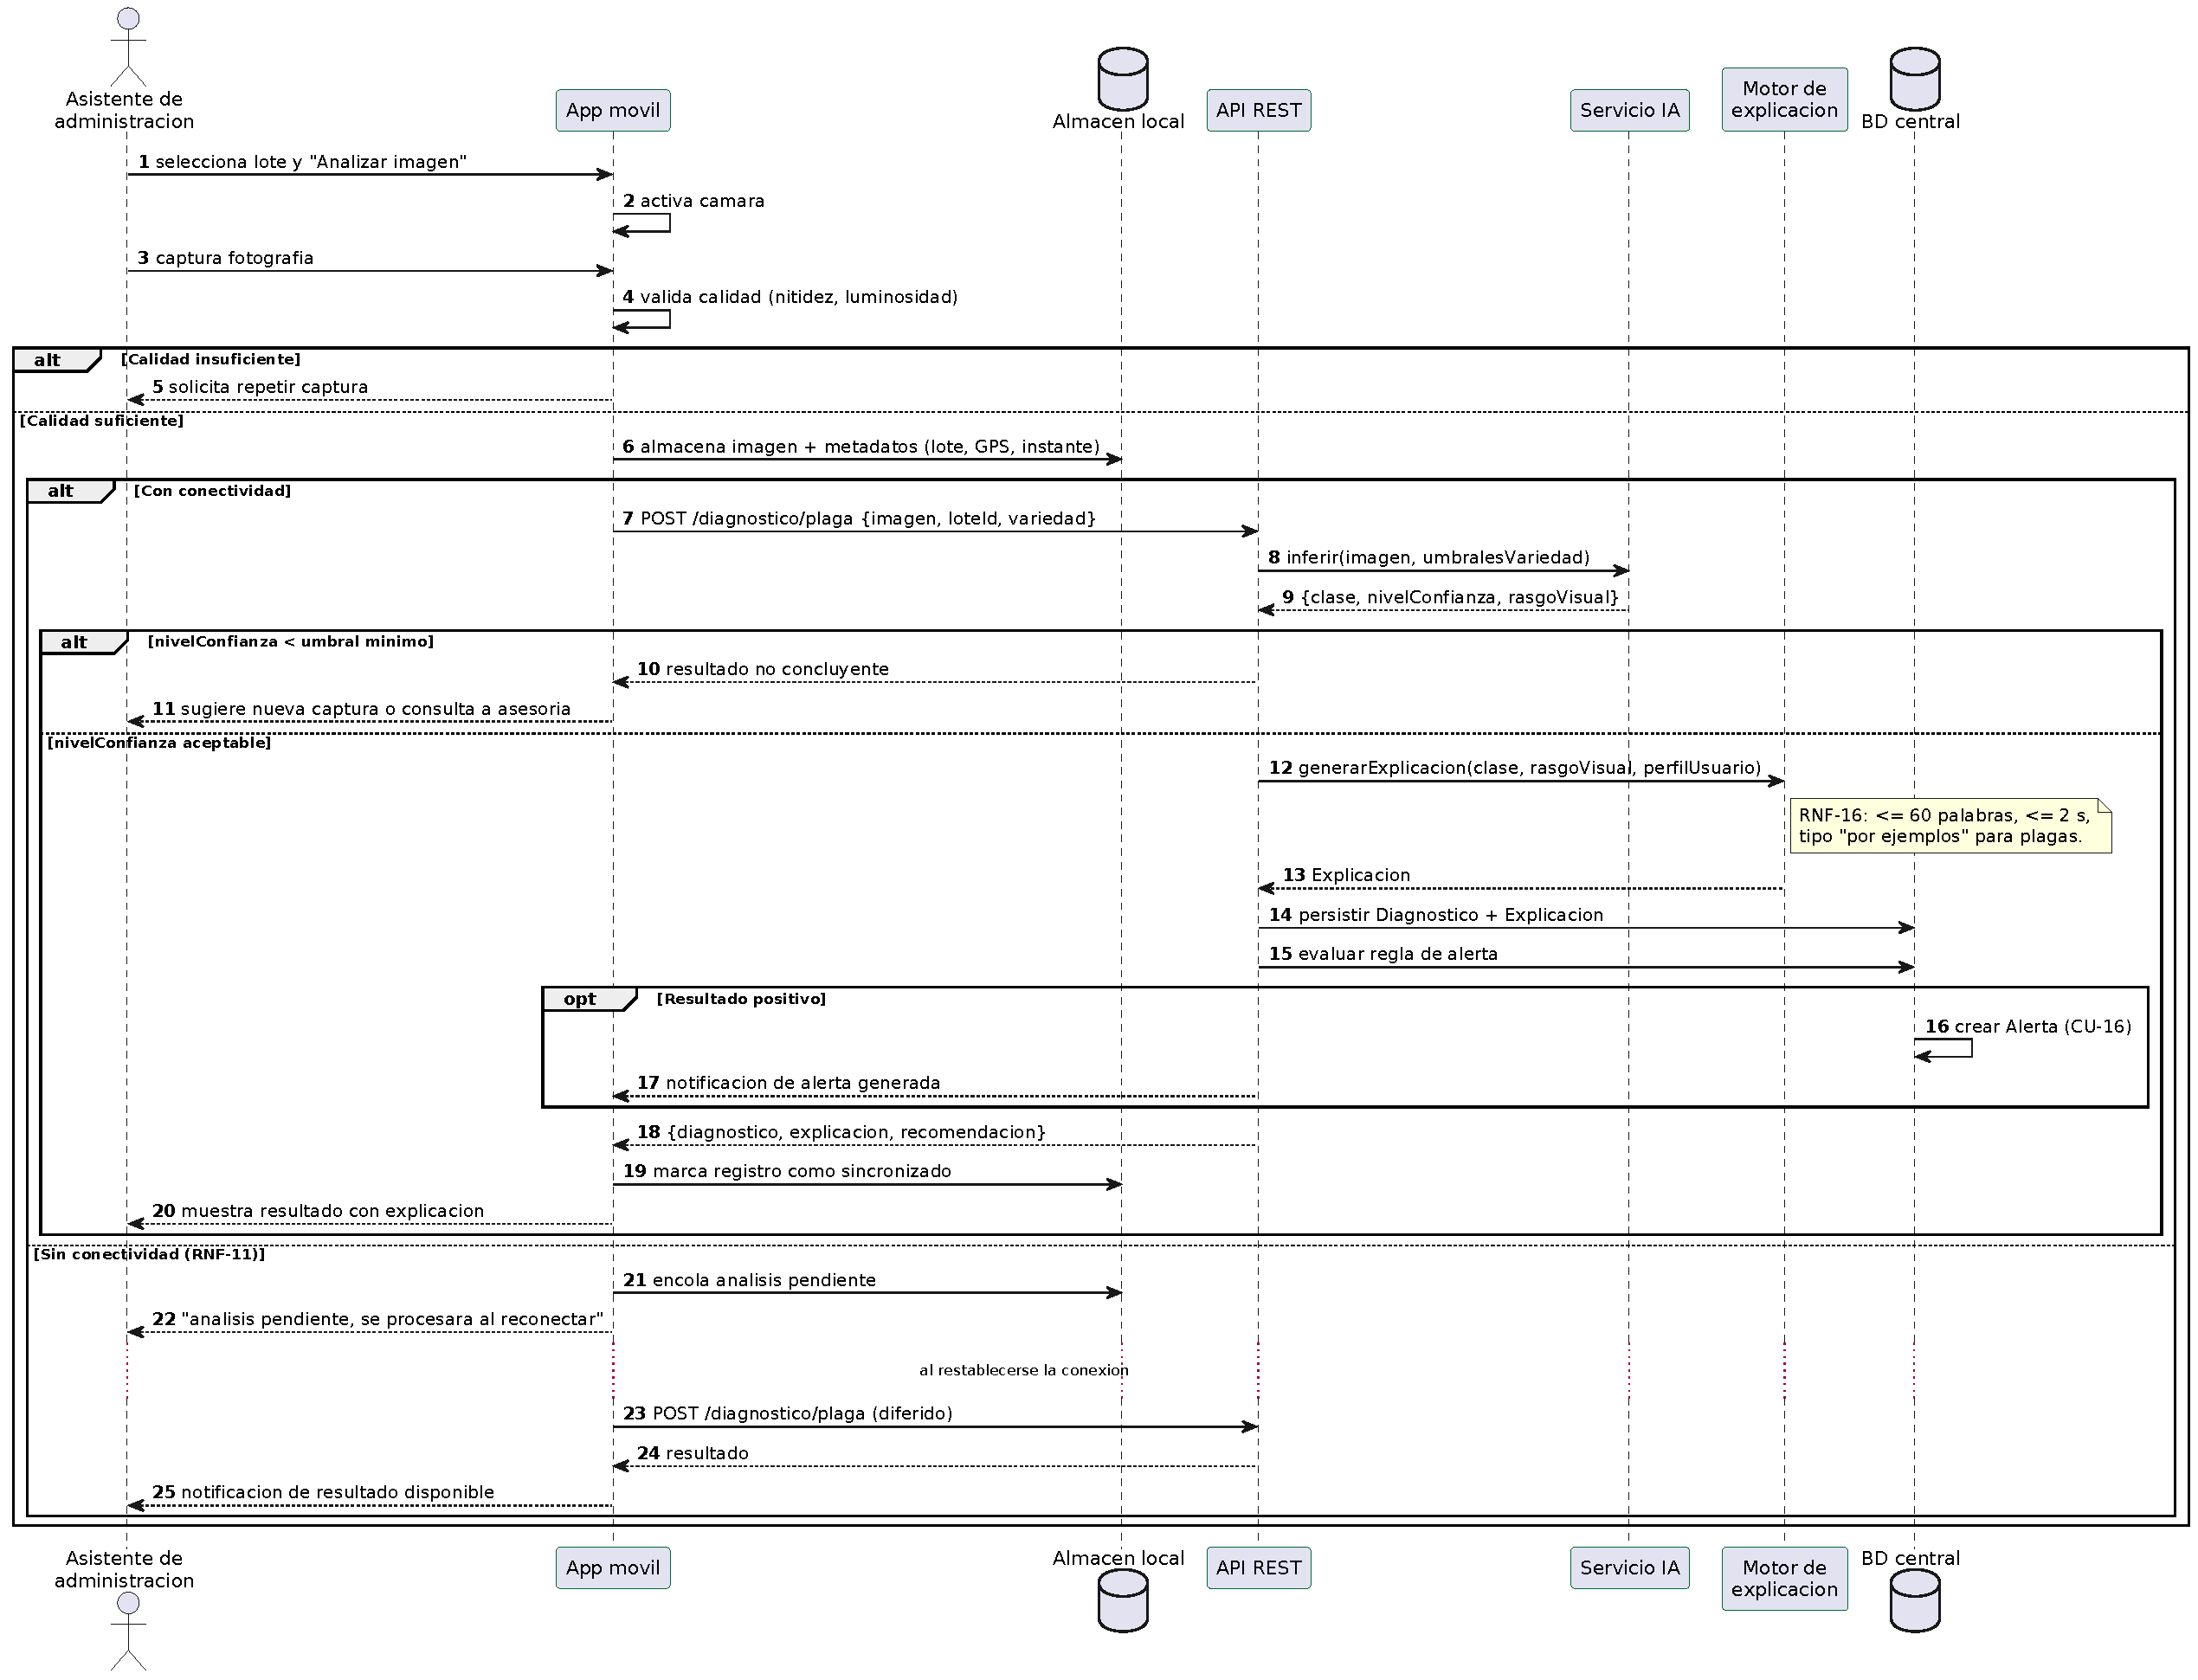
\includegraphics[width=1.0\textwidth]{img/secuencia_CU01}
\caption{Diagrama de secuencia del CU-01: análisis de imagen para detección de plaga, con las ramas de baja confianza y de operación sin conectividad.}
\label{fig:seq01}
\end{figure}

\begin{figure}[!htbp]
\centering
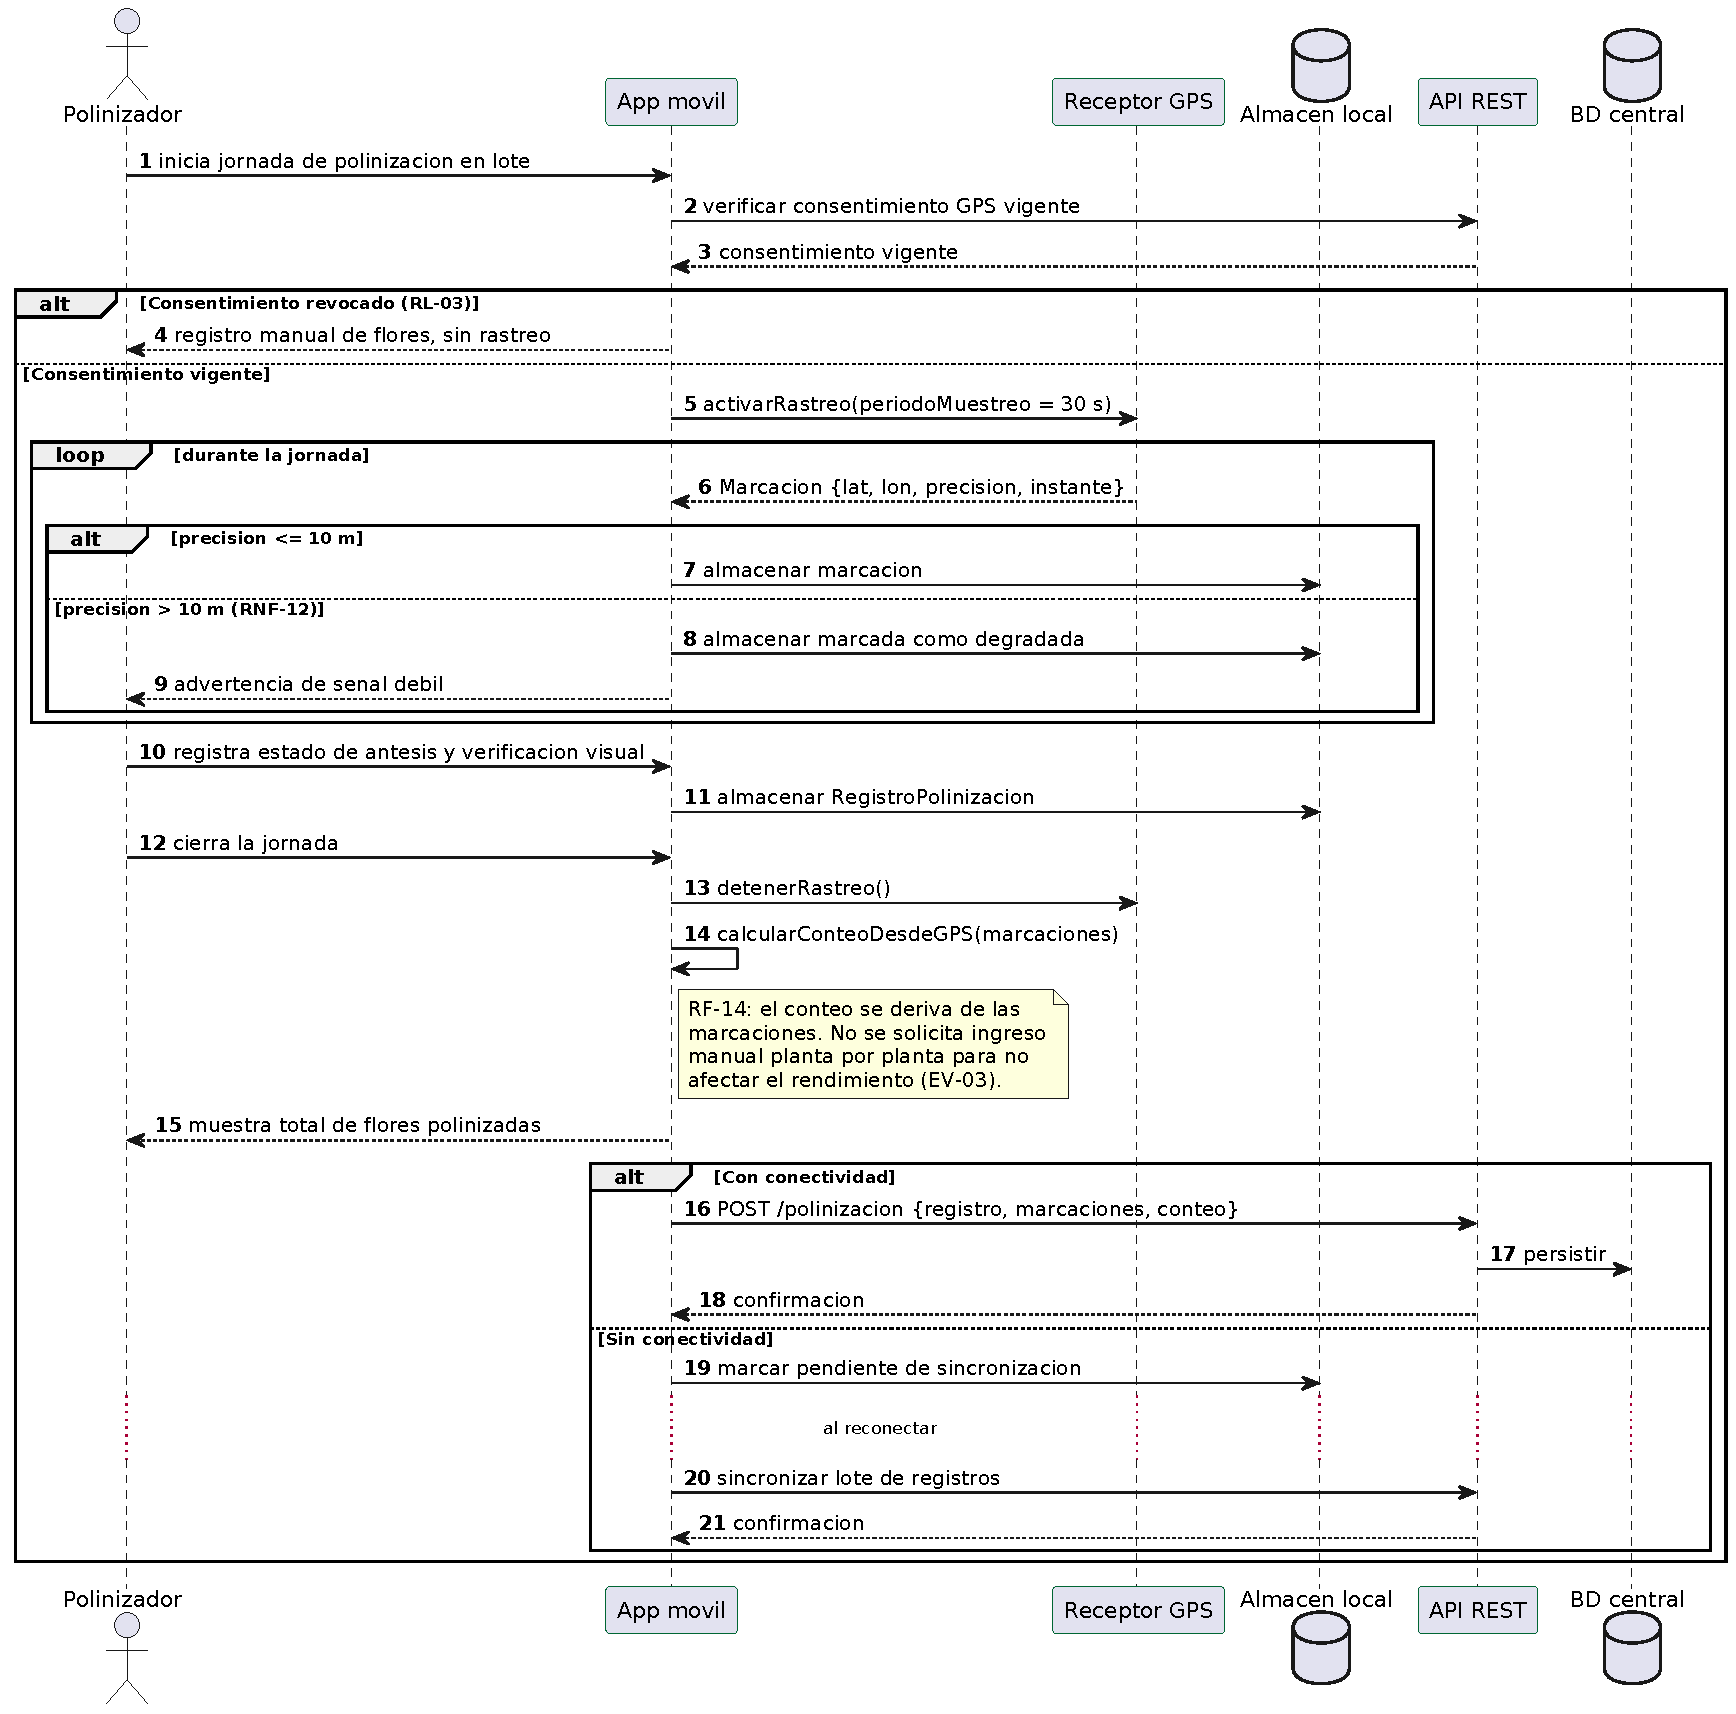
\includegraphics[width=1.0\textwidth]{img/secuencia_CU03}
\caption{Diagrama de secuencia del CU-03: registro de polinización y conteo georreferenciado, con verificación de consentimiento y manejo de precisión degradada.}
\label{fig:seq03}
\end{figure}

\begin{figure}[!htbp]
\centering
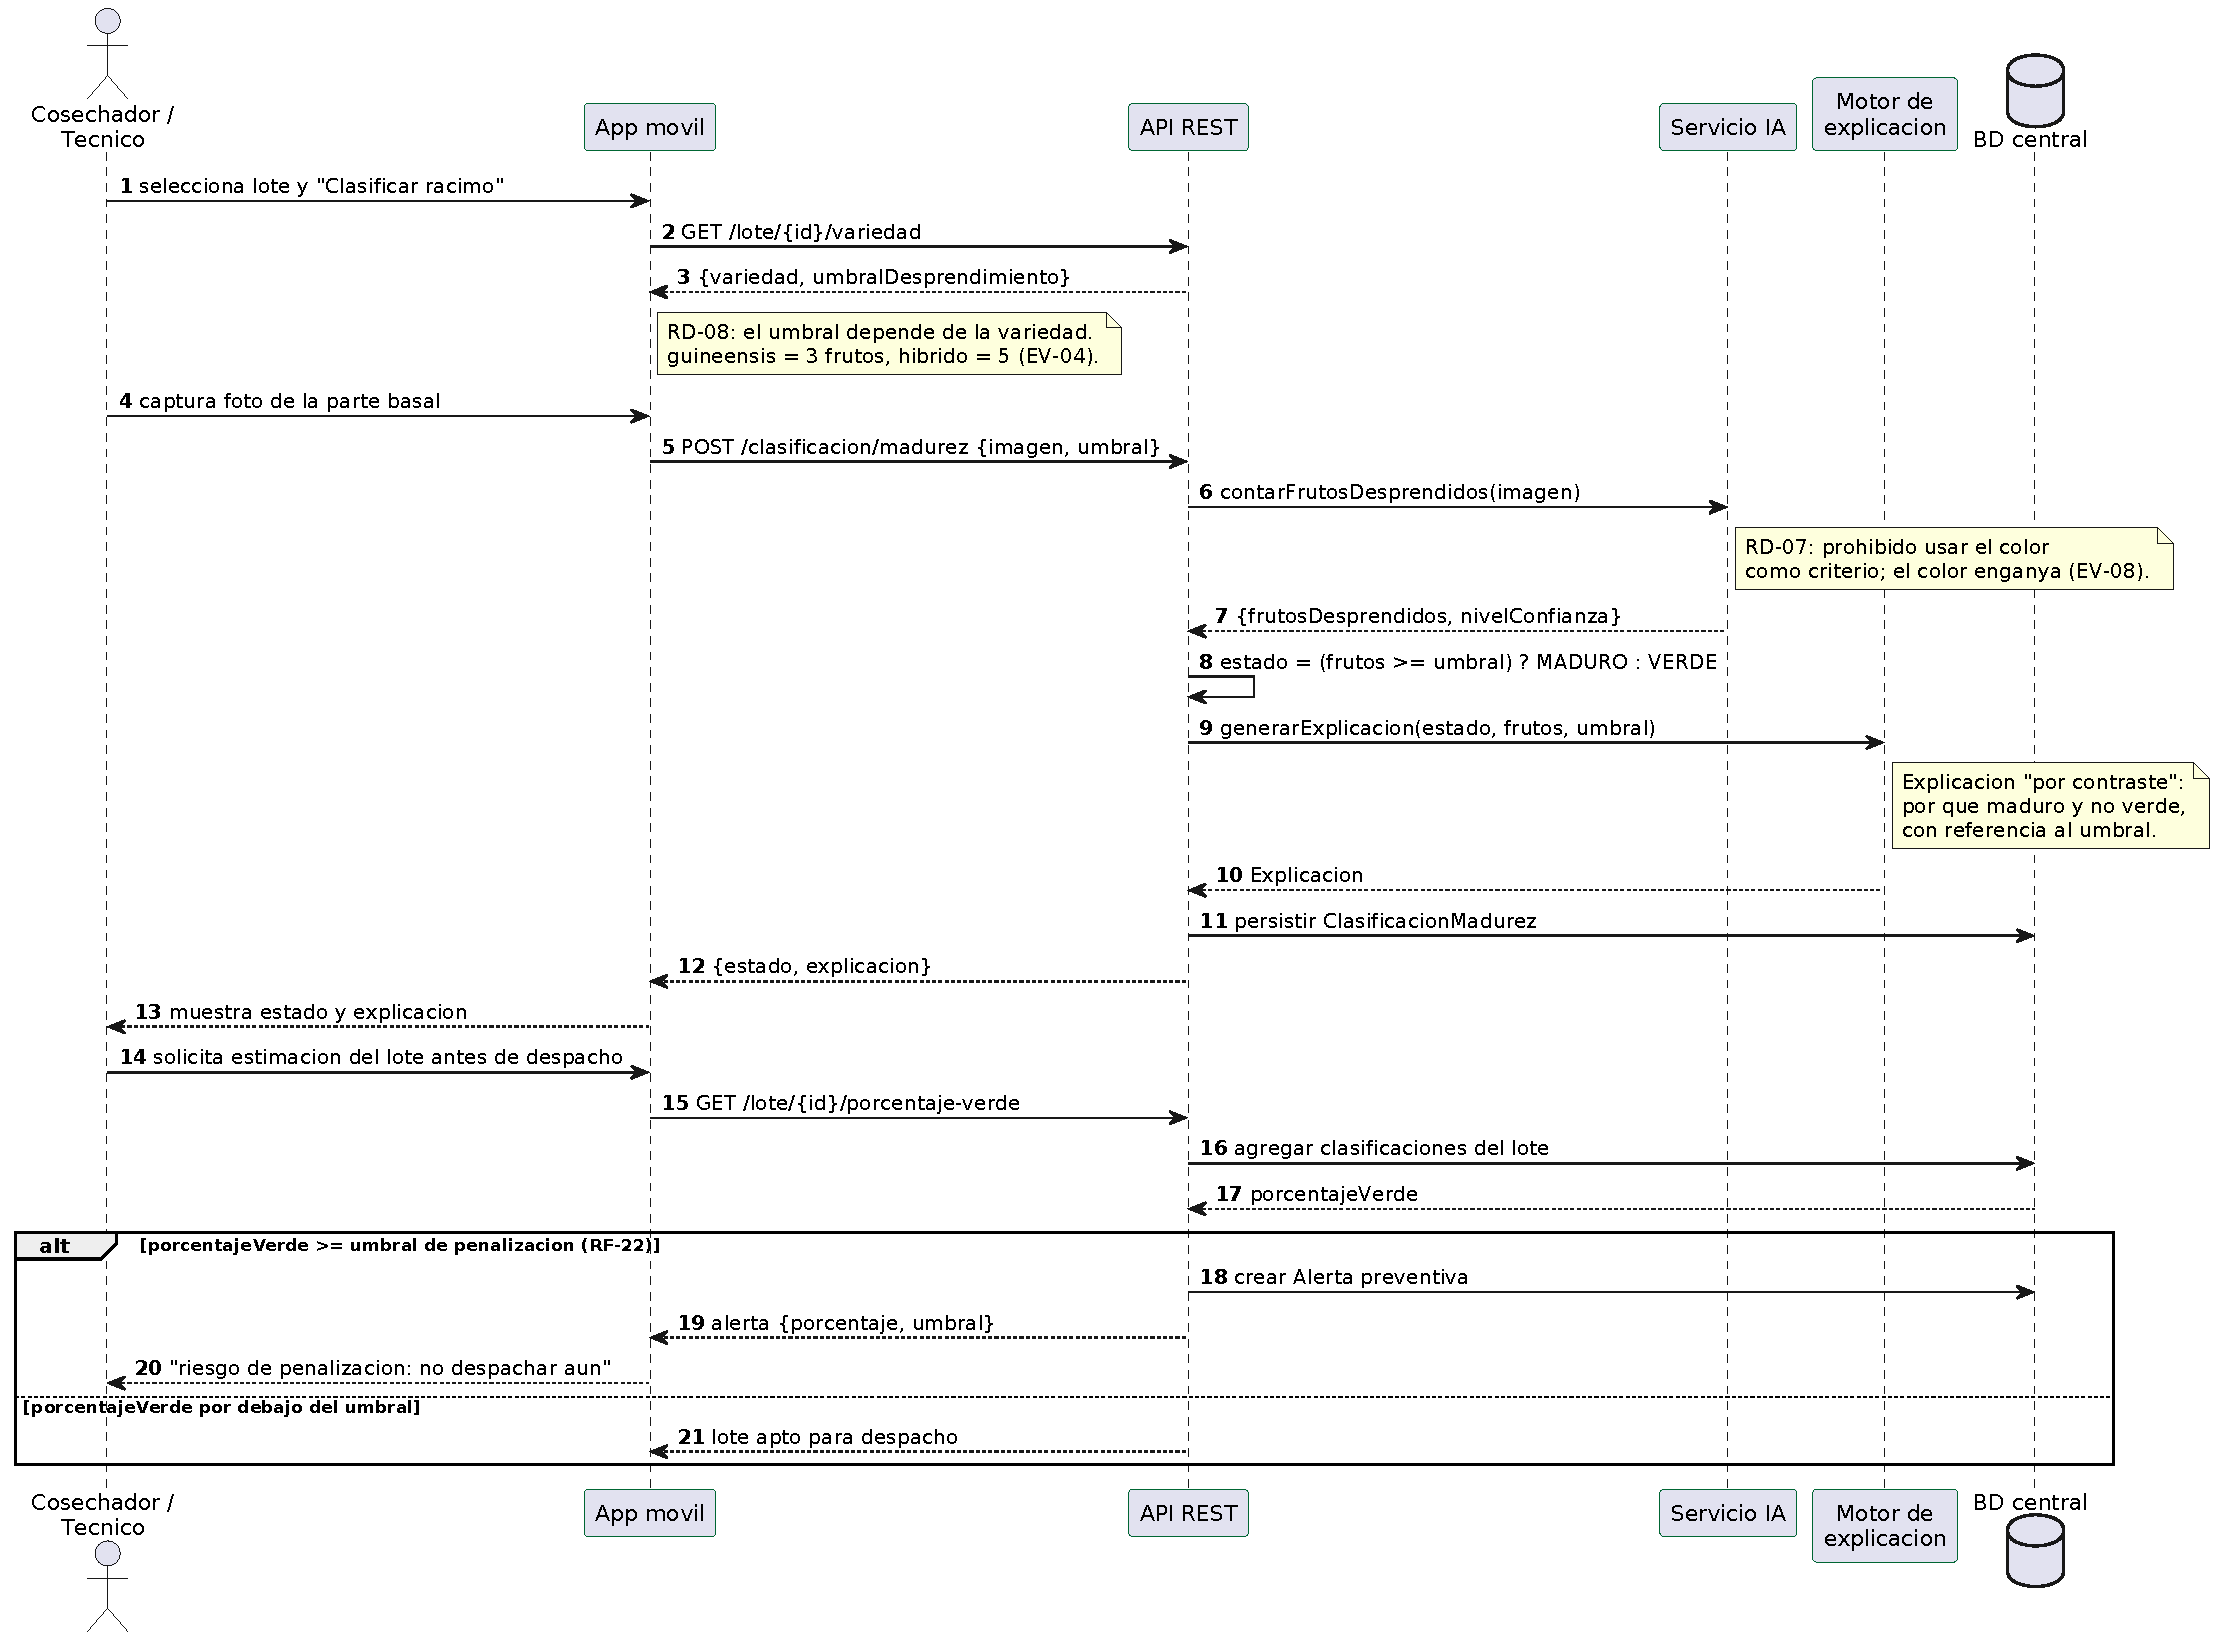
\includegraphics[width=1.0\textwidth]{img/secuencia_CU06}
\caption{Diagrama de secuencia del CU-06: clasificación de madurez del racimo y alerta preventiva de porcentaje de fruta verde.}
\label{fig:seq06}
\end{figure}

% ---------------------------------------------------------------------
\subsection{Diagrama de actividad}

El diagrama modela el ciclo semanal completo de planificación y ejecución, que constituye el proceso
central de la organización según los documentos operativos (\id{EV-11}). Incorpora la bifurcación
por disponibilidad de dispositivo (\id{RF-35}), la bifurcación por conectividad (\id{RNF-11}) y el
mecanismo de arrastre de labor incompleta (\id{RF-27}).

\begin{figure}[!htbp]
\centering
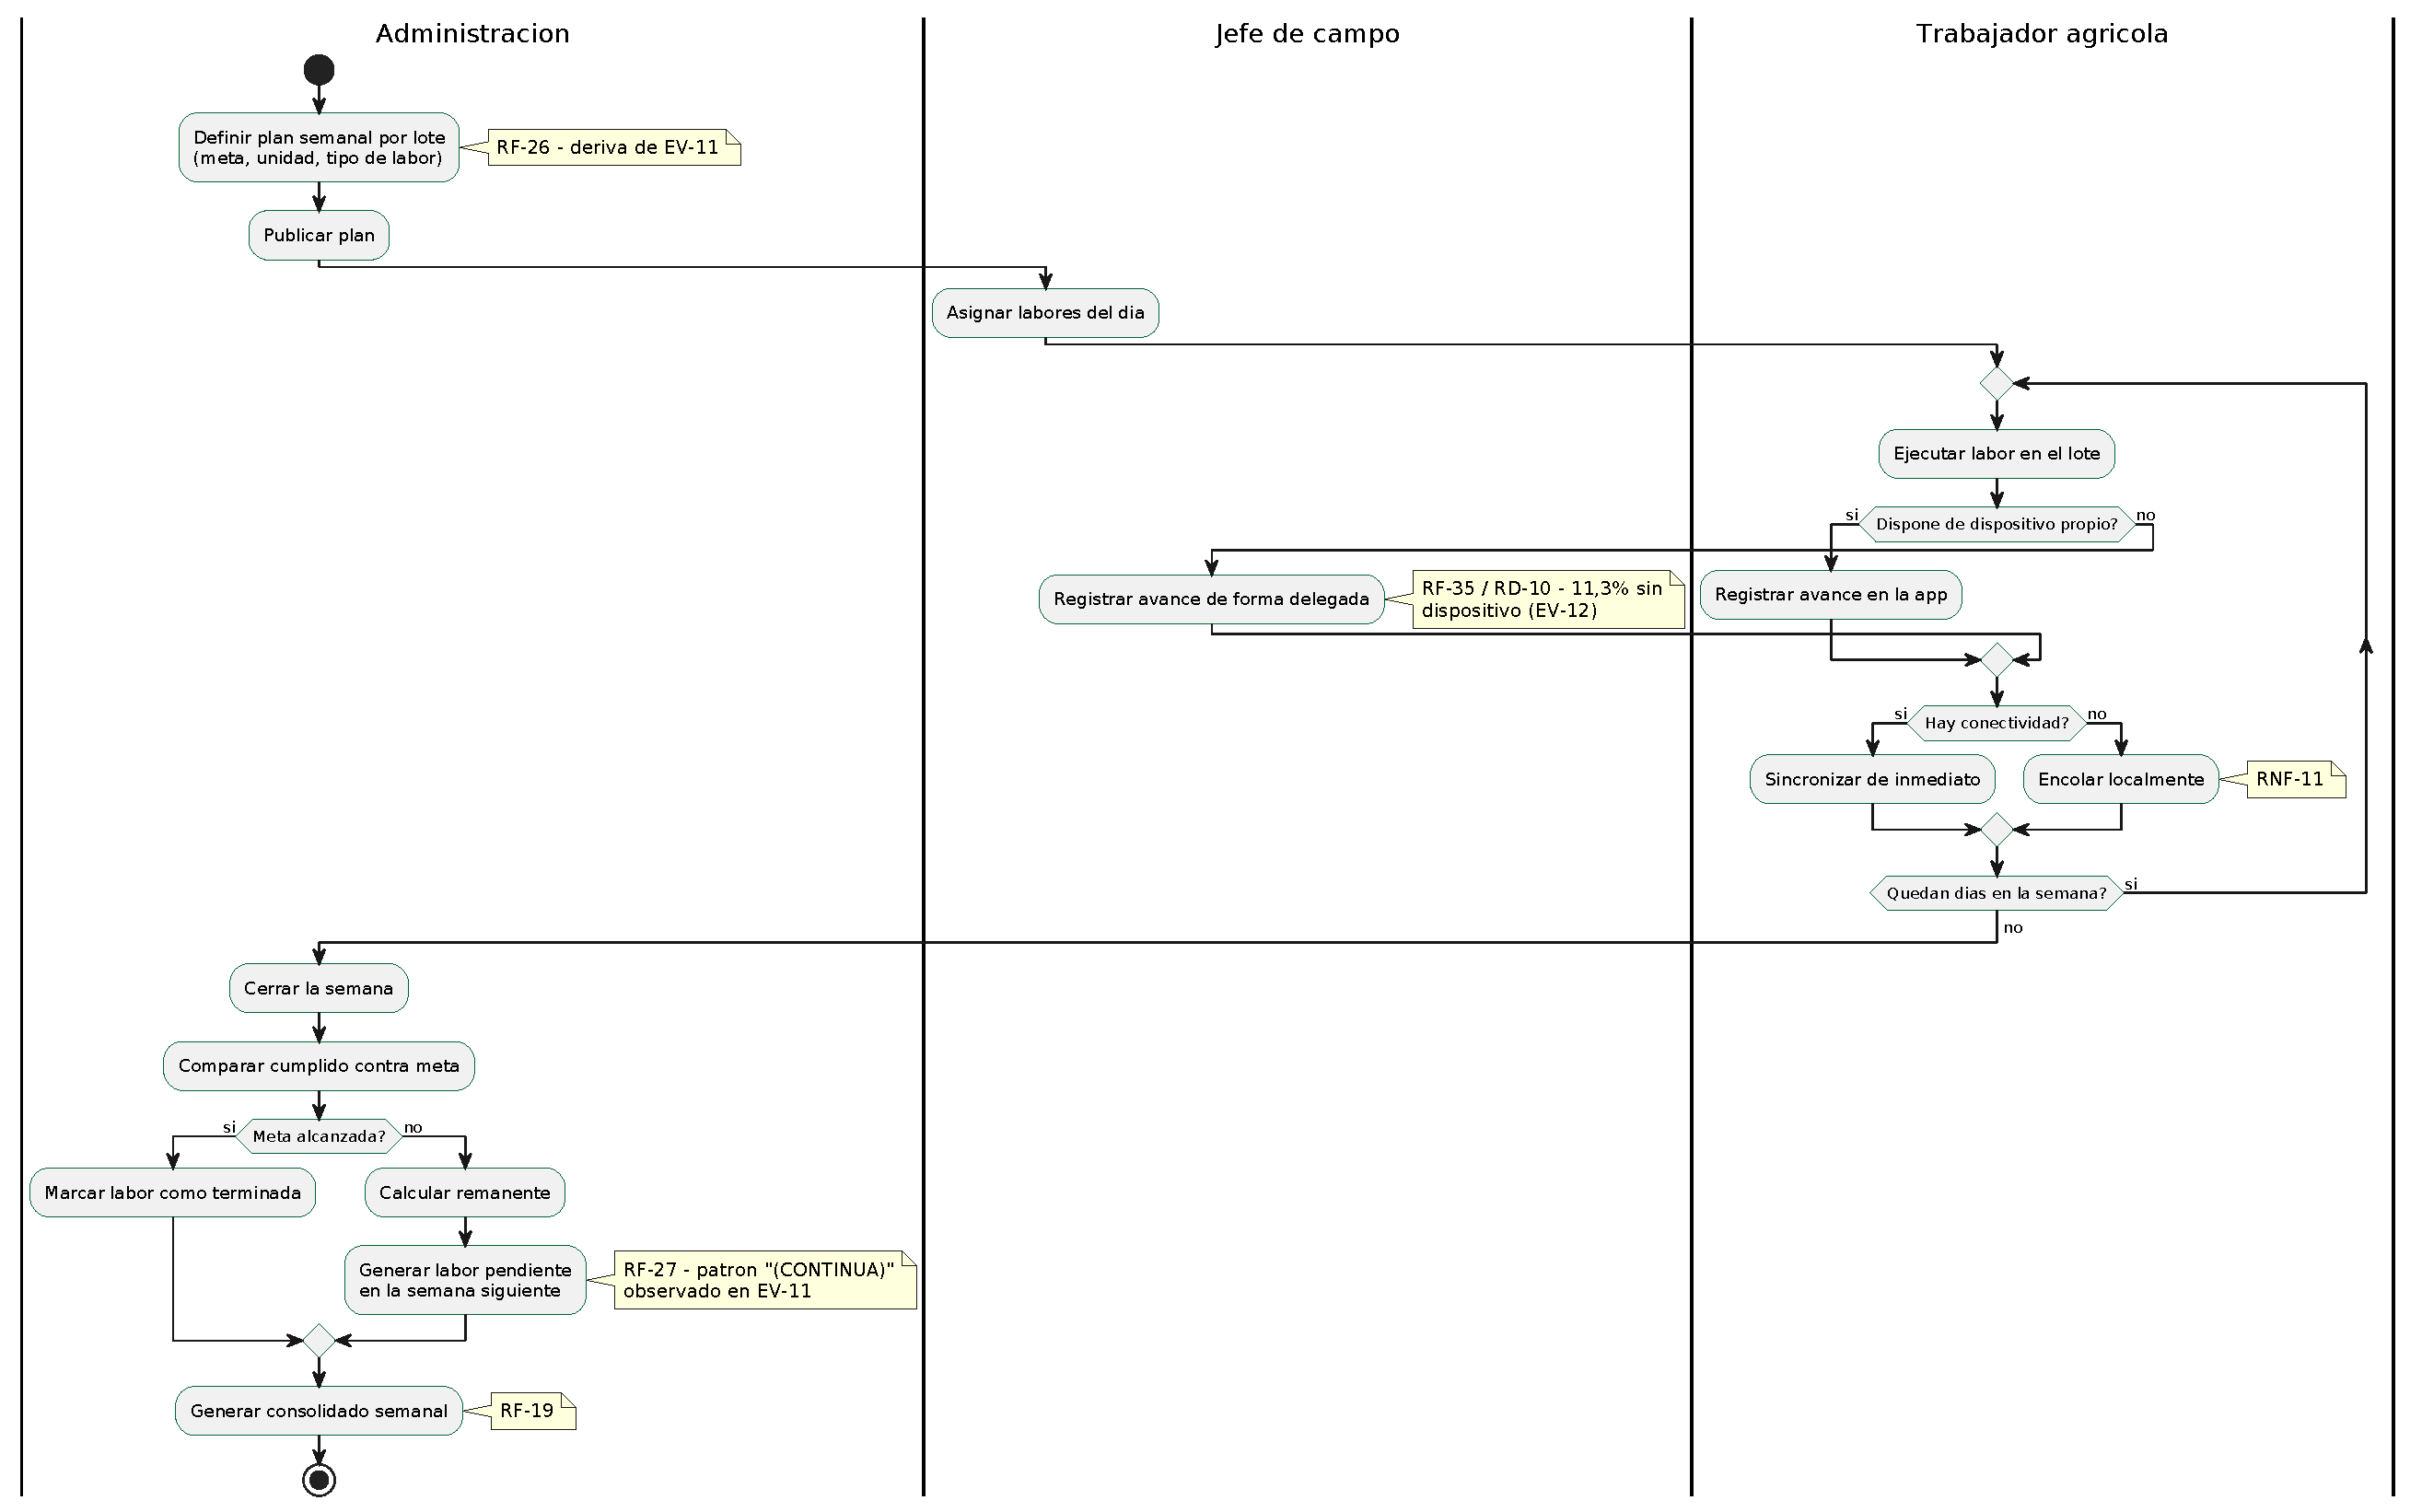
\includegraphics[width=1.0\textwidth]{img/actividad_ciclo_semanal}
\caption{Diagrama de actividad del ciclo semanal de planificación y ejecución de labores.}
\label{fig:actividad}
\end{figure}

% ---------------------------------------------------------------------
\subsection{Diagramas de estados}

Se modelan las dos entidades del dominio con ciclo de vida no trivial: el \textbf{racimo}, cuya
trayectoria determina el valor económico de la producción, y la \textbf{alerta}, cuyo ciclo refleja
la latencia real de verificación documentada en \id{EV-07}.

\begin{figure}[!htbp]
\centering
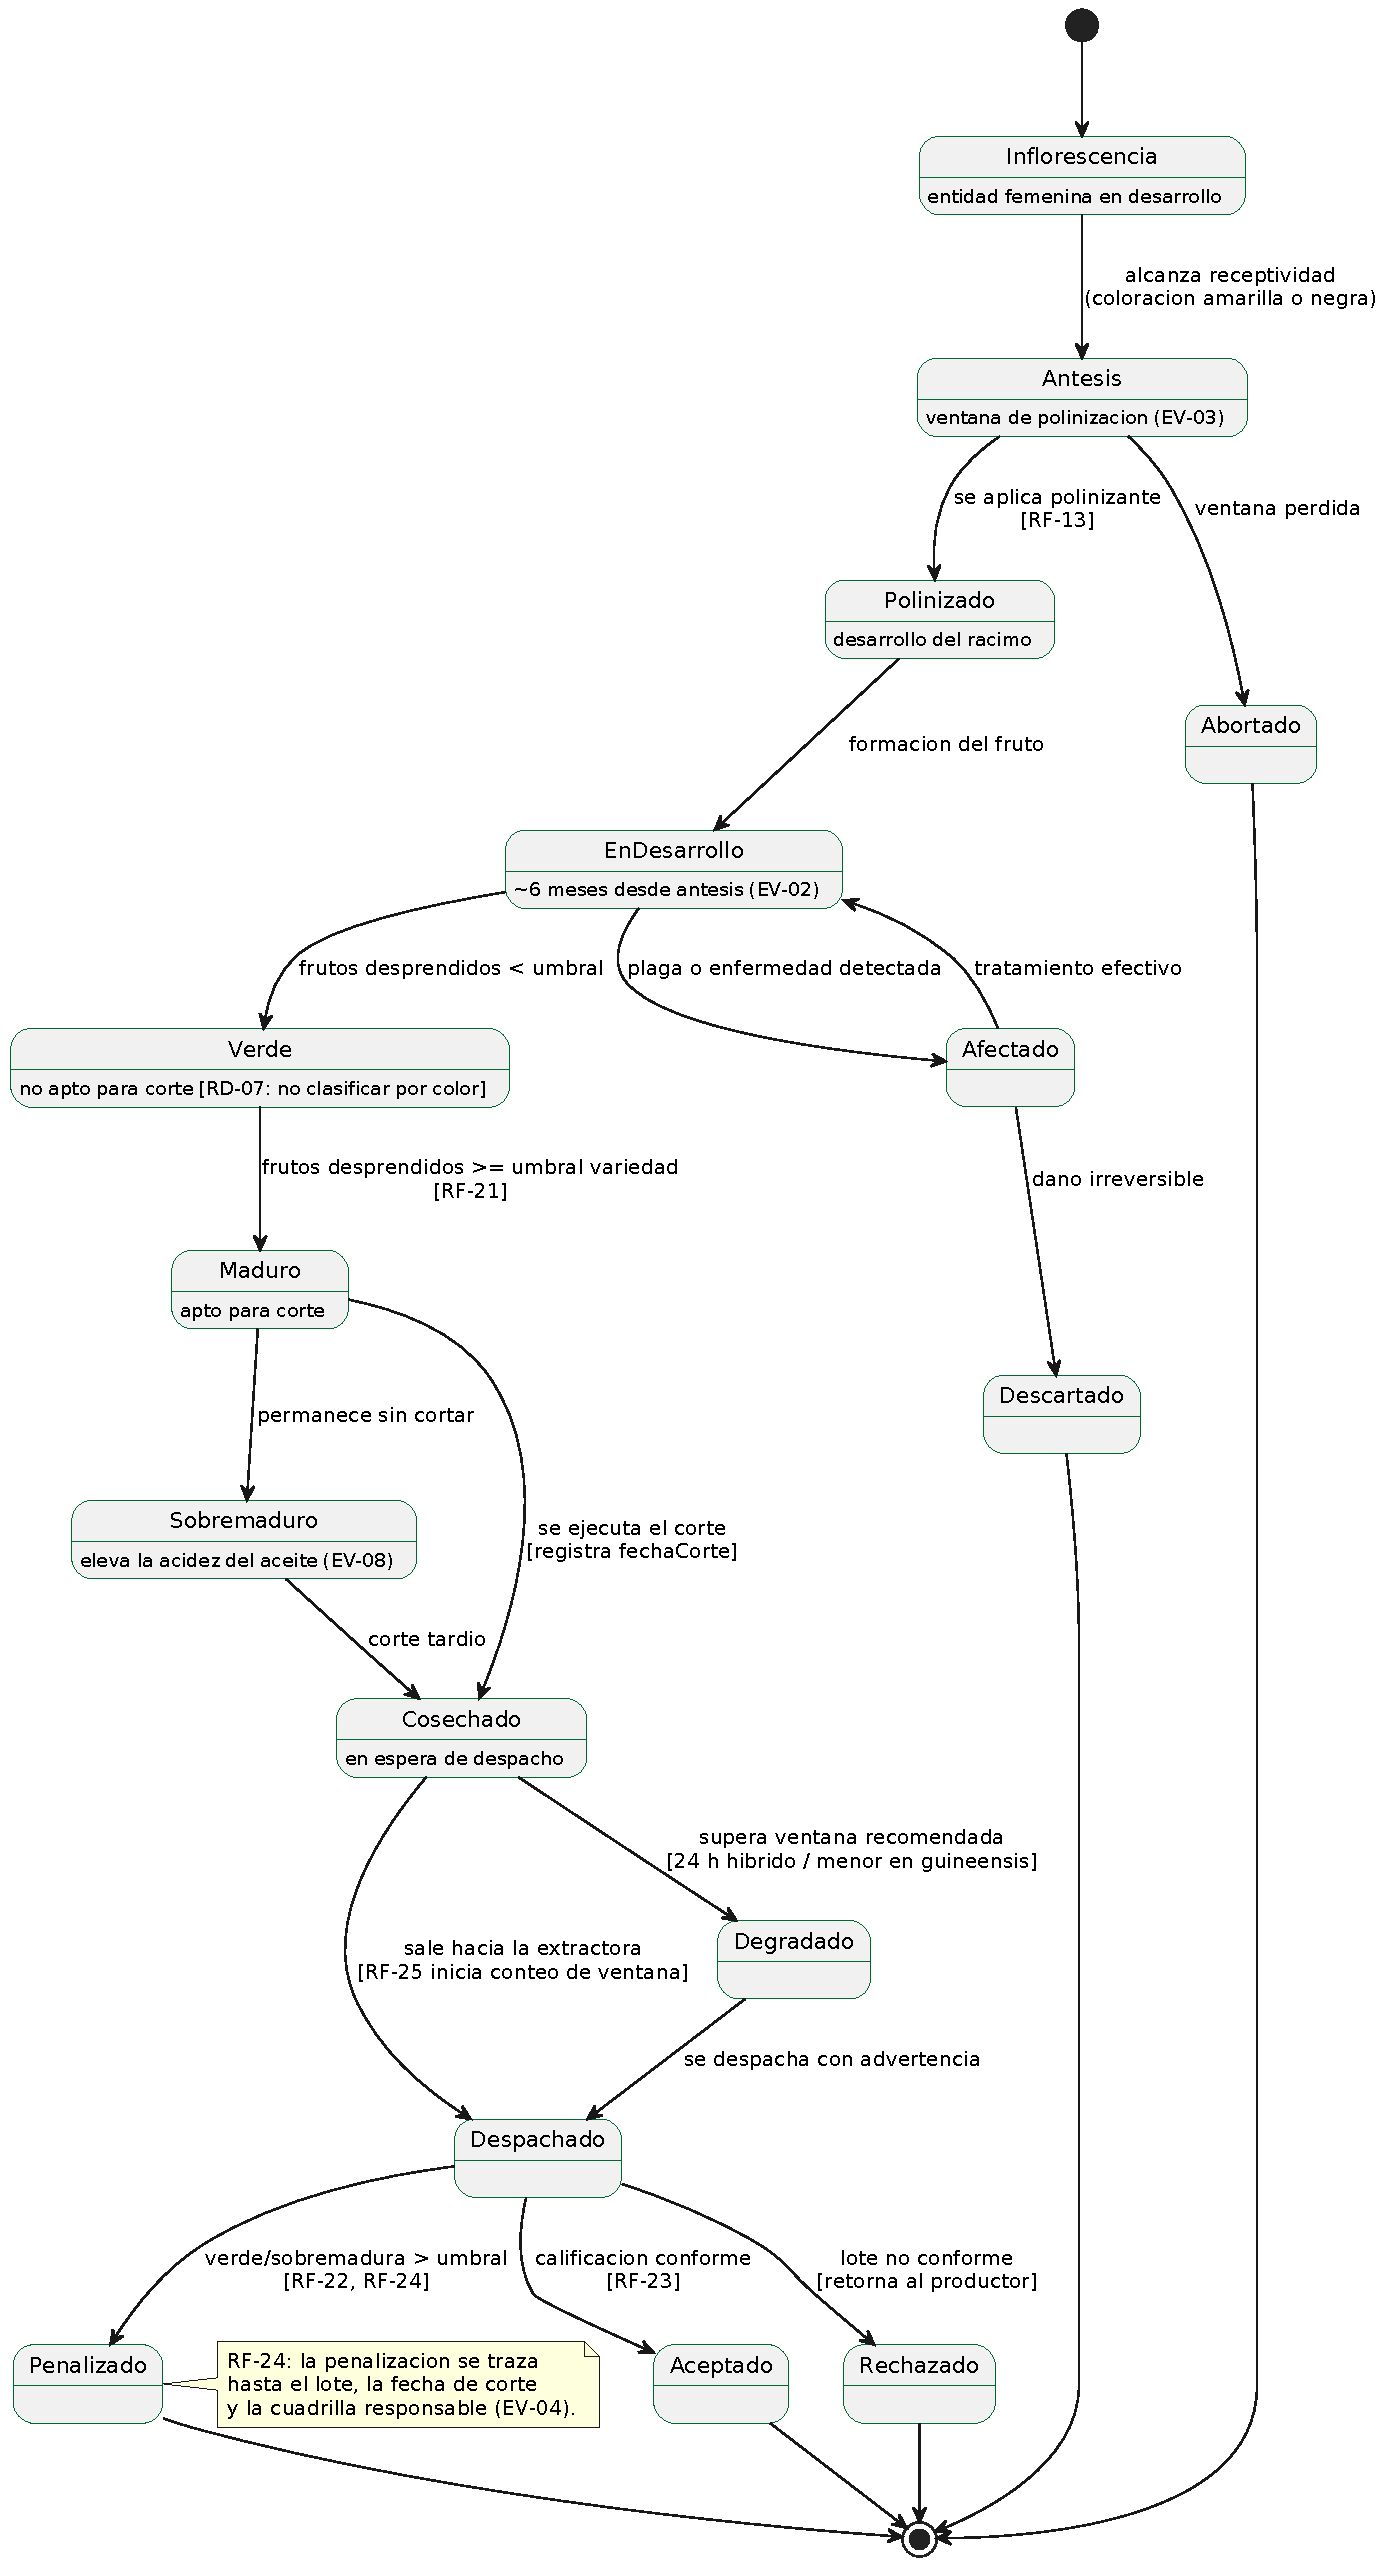
\includegraphics[width=0.67\textwidth]{img/estados_racimo}
\caption{Diagrama de estados del racimo, desde la inflorescencia hasta la calificación en la planta extractora.}
\label{fig:est_racimo}
\end{figure}

\begin{figure}[!htbp]
\centering
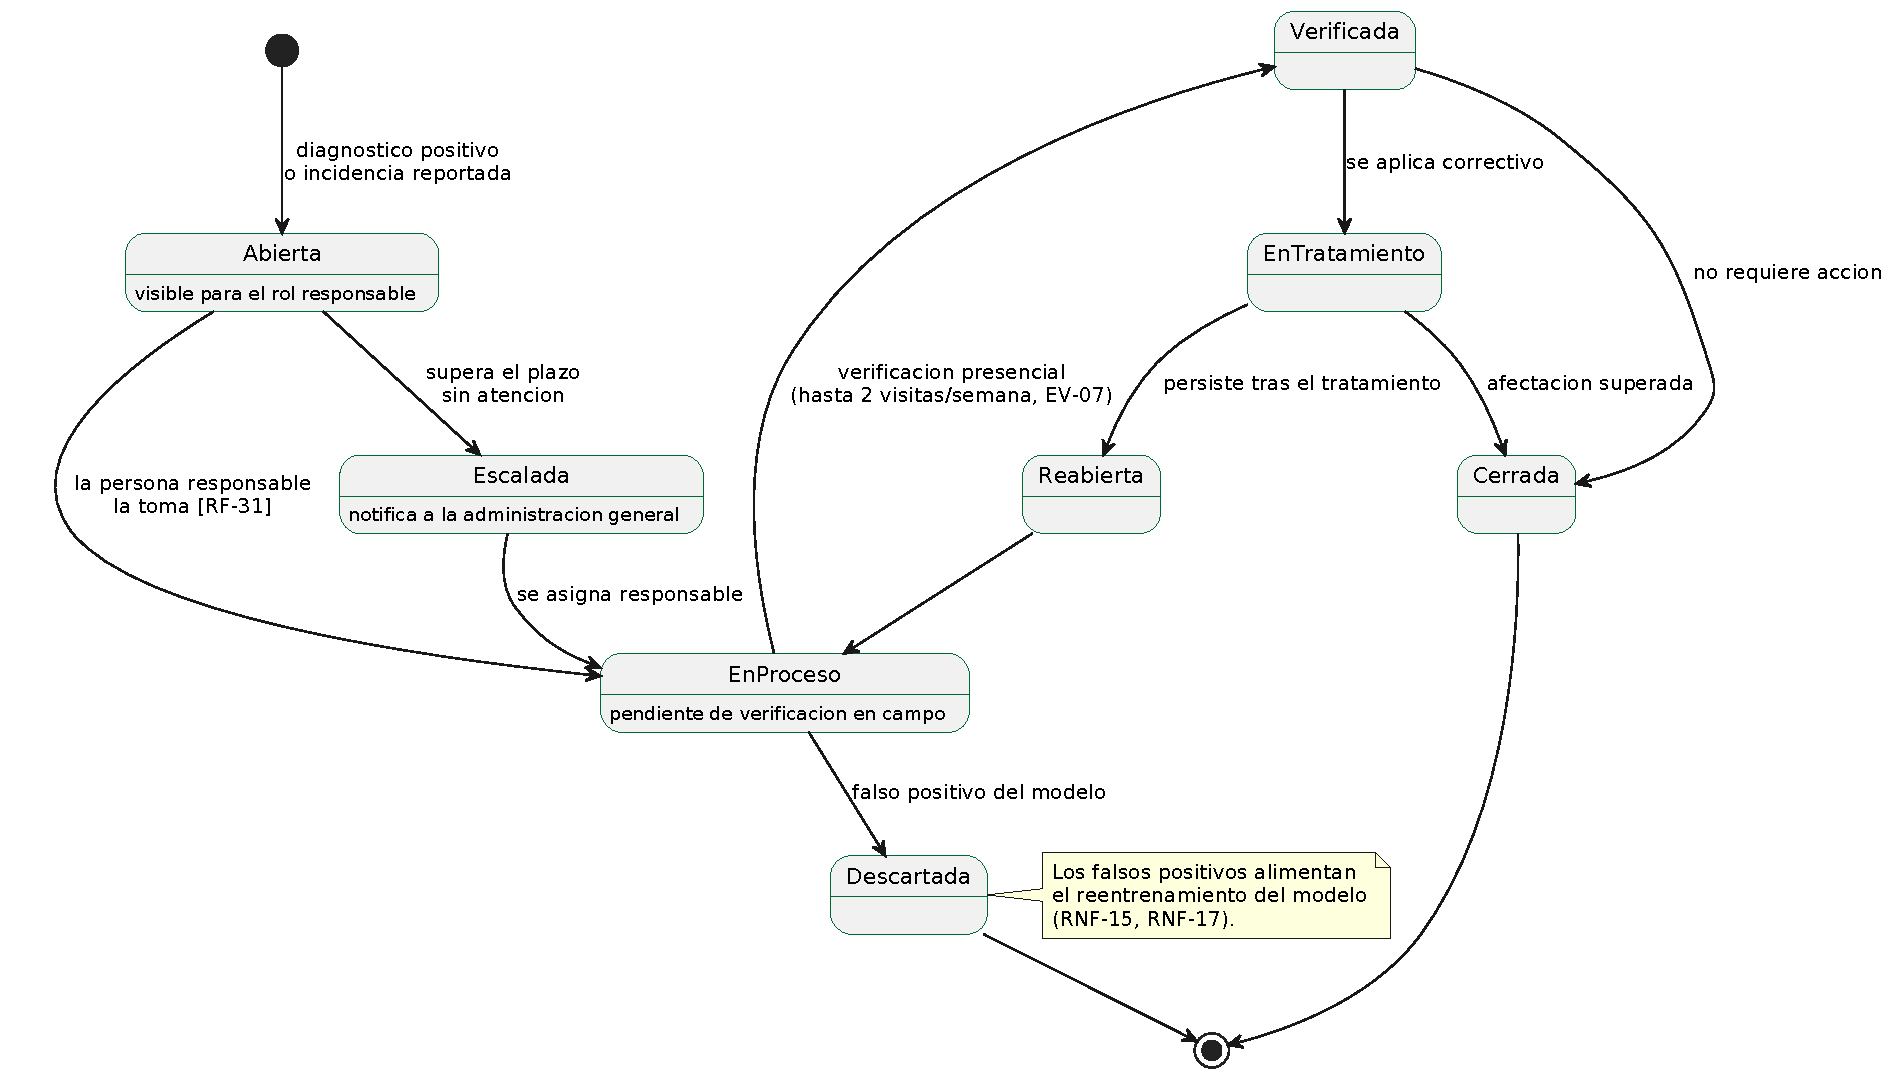
\includegraphics[width=1.0\textwidth]{img/estados_alerta}
\caption{Diagrama de estados de la alerta, con escalamiento por vencimiento de plazo y reapertura tras tratamiento inefectivo.}
\label{fig:est_alerta}
\end{figure}

\noindent
El estado \emph{Degradado} del racimo materializa el hallazgo de \id{EV-04} sobre la ventana entre
corte y entrega: el material híbrido tolera un intervalo mayor por su contenido de antioxidantes,
mientras que el \emph{guineensis} se deshidrata en dos o tres días. El estado \emph{Descartada} de
la alerta corresponde a los falsos positivos del modelo y alimenta el ciclo de reentrenamiento
previsto en \id{RNF-15} y \id{RNF-17}.

% ---------------------------------------------------------------------
\subsection{Diagrama de componentes}

\begin{figure}[!htbp]
\centering
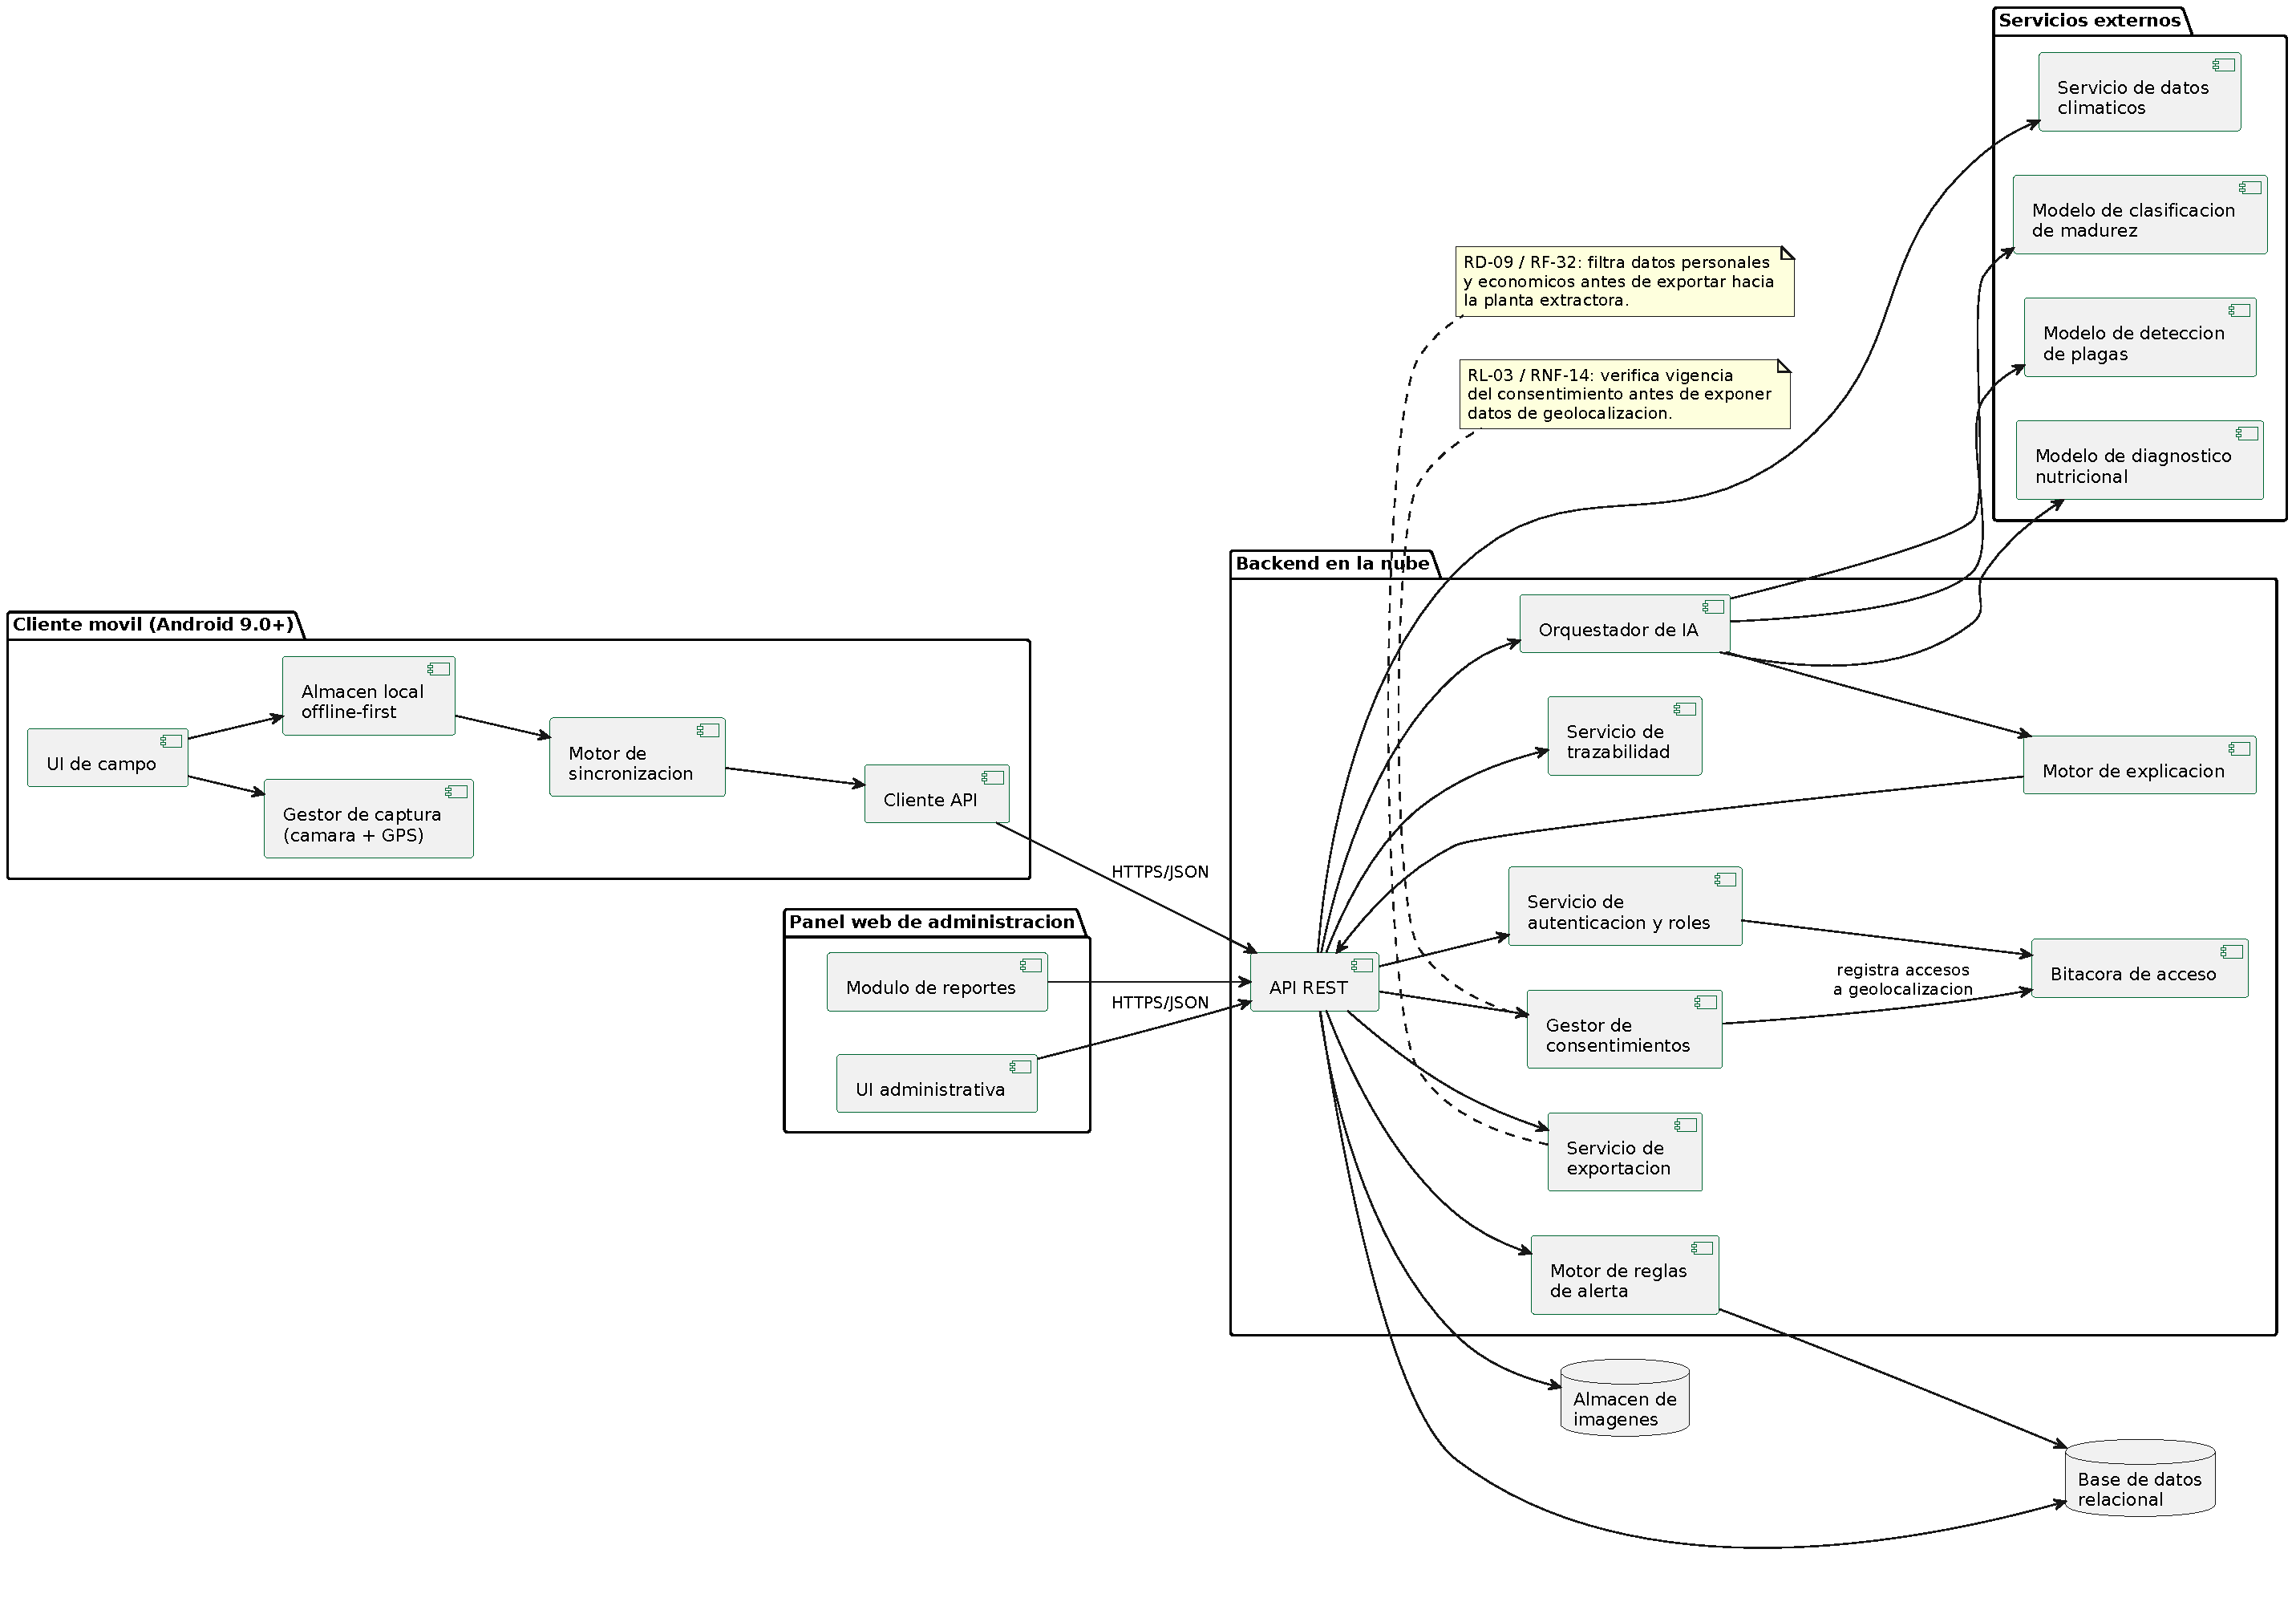
\includegraphics[width=1.0\textwidth]{img/componentes}
\caption{Diagrama de componentes del SIMPA.}
\label{fig:componentes}
\end{figure}

\noindent
Dos componentes merecen mención explícita por su origen normativo. El \emph{gestor de
consentimientos} verifica la vigencia antes de exponer cualquier dato de geolocalización y registra
todo acceso en la bitácora (\id{RL-03}, \id{RNF-14}). El \emph{servicio de exportación} filtra los
datos personales y económicos antes de generar el archivo destinado a la planta extractora
(\id{RD-09}, \id{RF-32}); su existencia como componente separado responde al criterio expreso de la
contraparte de que hay información que no puede compartirse (\id{EV-04}).

% ---------------------------------------------------------------------
\subsection{Diagrama de despliegue}

\begin{figure}[!htbp]
\centering
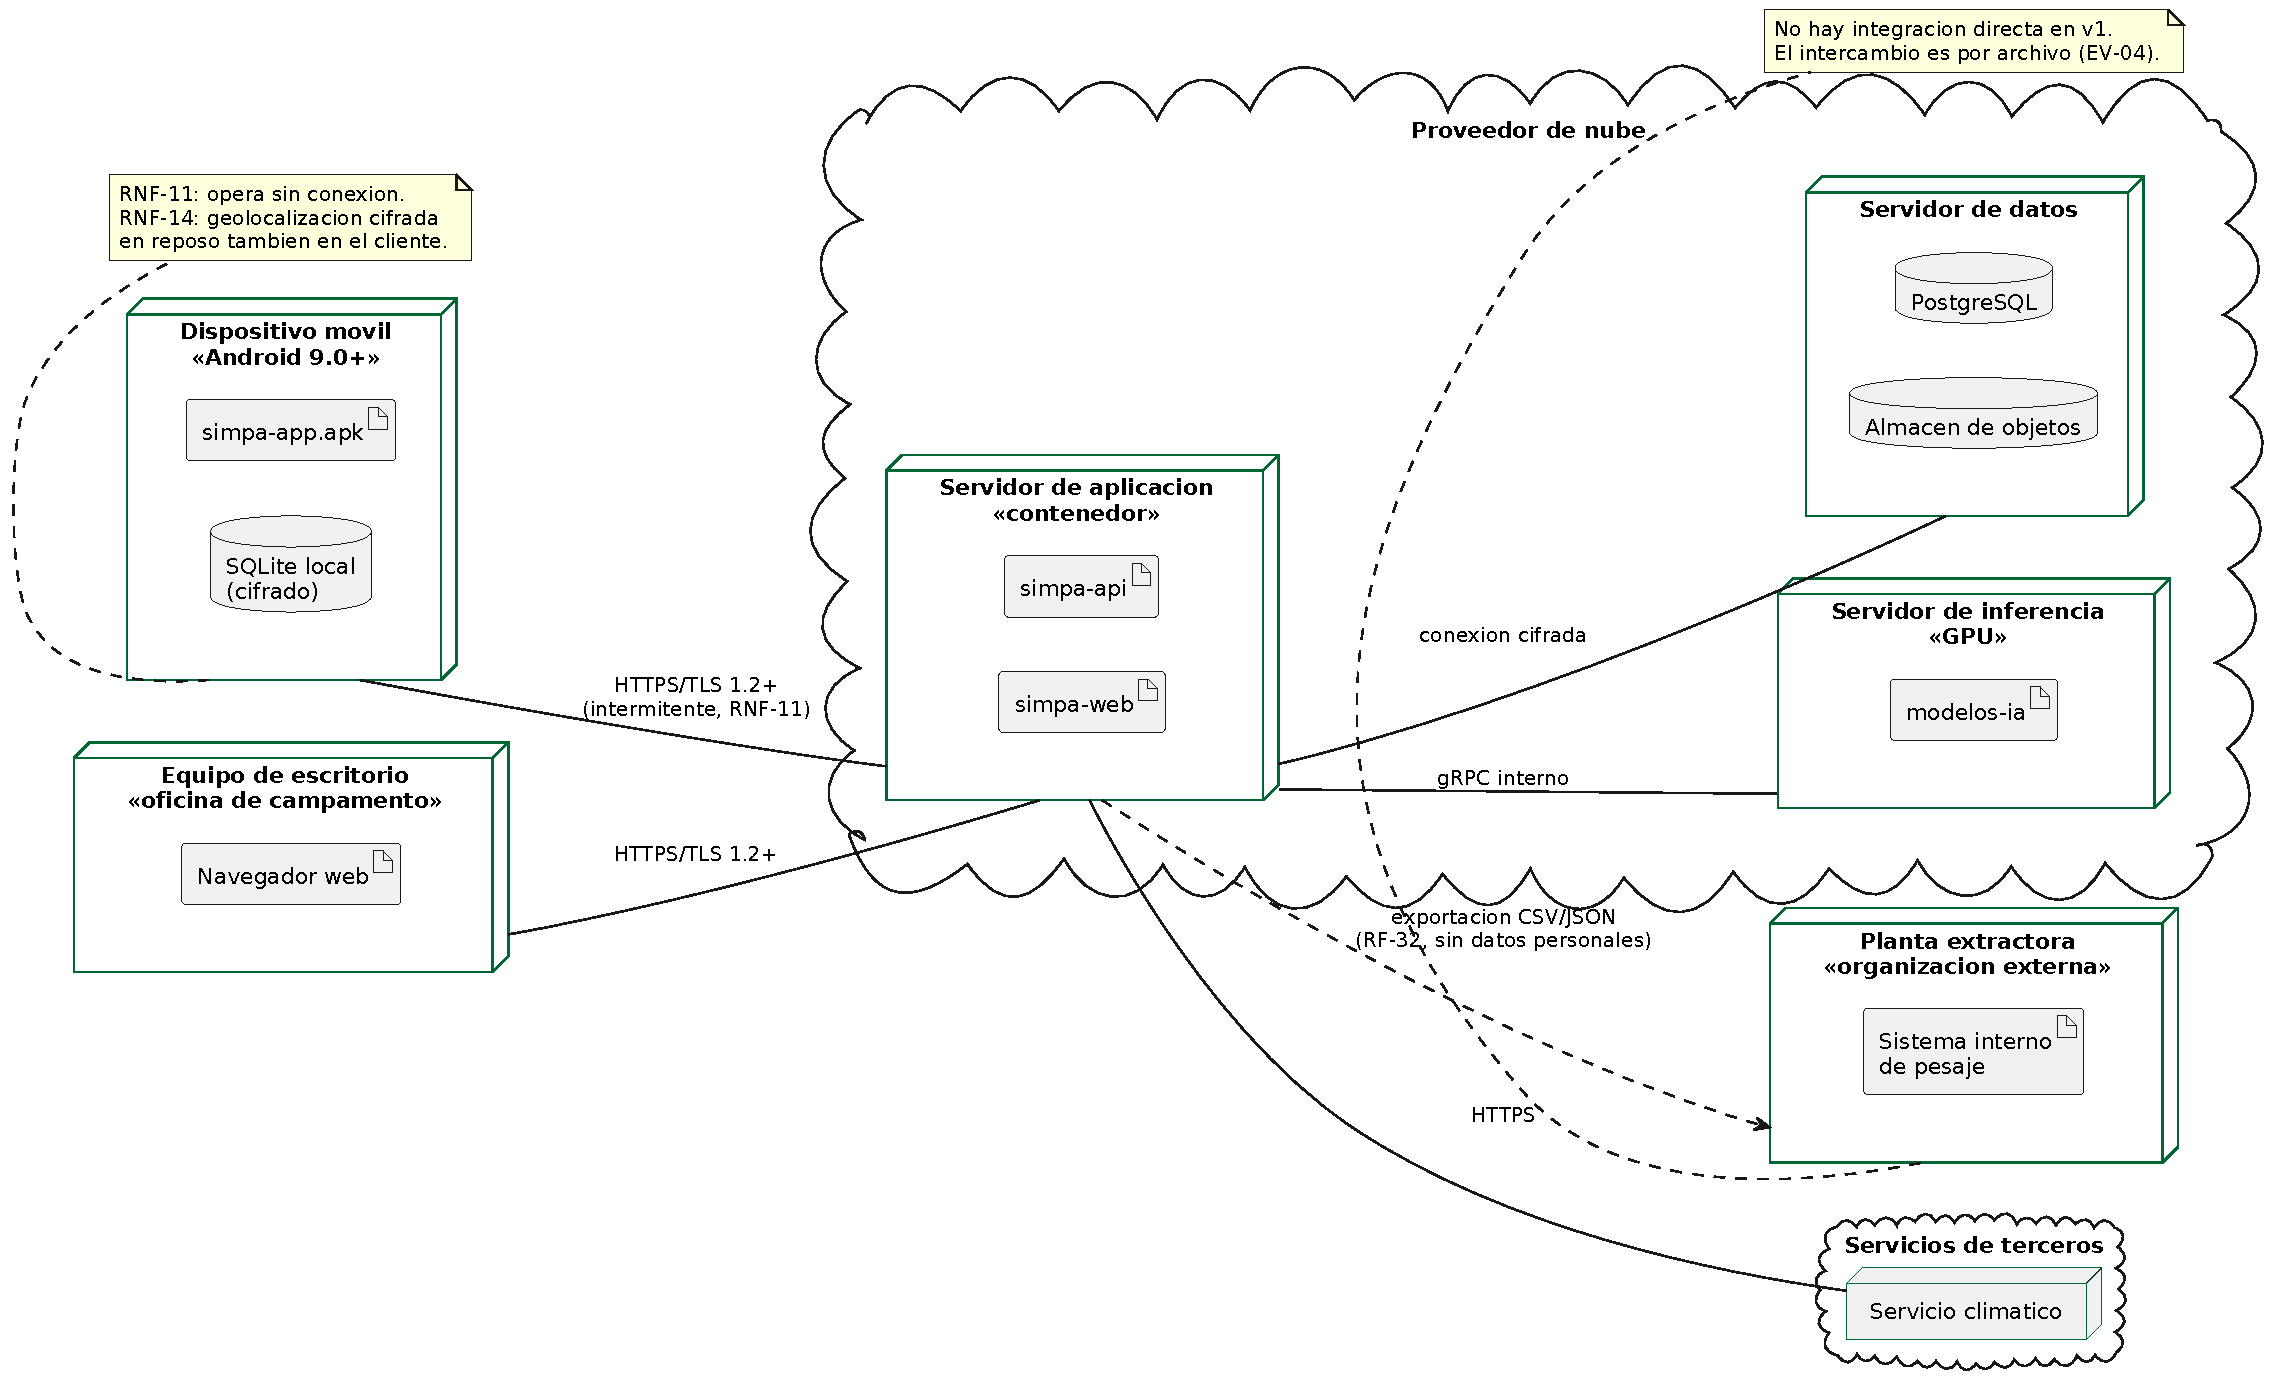
\includegraphics[width=1.0\textwidth]{img/despliegue}
\caption{Diagrama de despliegue del SIMPA.}
\label{fig:despliegue}
\end{figure}

\noindent
El enlace entre el dispositivo móvil y el servidor de aplicación se declara explícitamente como
\emph{intermitente}: el 74{,}2\% de las personas destinatarias no dispone de conectividad permanente
(\id{EV-12}). La planta extractora se representa como nodo externo sin integración directa; el
intercambio en la versión v1 se realiza por archivo, conforme a \id{RF-32}.

% ---------------------------------------------------------------------
\subsection{Cobertura del modelado}

\begin{longtable}{|L{4.6cm}|C{2.2cm}|C{2.2cm}|L{5.0cm}|}
\hline
\rowcolor{grisclaro}\textbf{Artefacto} & \textbf{Exigido} & \textbf{Entregado} & \textbf{Observación} \\
\hline
\endhead
Diagrama de casos de uso general & 1 & 1 & 8 actores, 18 casos de uso \\ \hline
Casos de uso detallados & 10 & 10 & Todos los \emph{Must}; $\geq 2$ flujos alternativos y $\geq 1$ excepción cada uno \\ \hline
Diagrama de clases refinado & 1 & 1 & 25 clases con atributos y operaciones \\ \hline
Diagramas de secuencia & CU \emph{Must} & 3 & CU-01, CU-03, CU-06 \\ \hline
Diagramas de actividad & Flujos principales & 1 & Ciclo semanal completo \\ \hline
Diagramas de estados & Entidades no triviales & 2 & Racimo y Alerta \\ \hline
Diagrama de componentes & 1 & 1 & --- \\ \hline
Diagrama de despliegue & 1 & 1 & --- \\ \hline
\caption{Cobertura del modelado UML frente a lo exigido en la §3.4 de la guía}
\end{longtable}

%  Requiere las imagenes en img/ generadas desde 03_Modelado/Diagramas_UML/
% =====================================================================

\newpage
\section{Modelado del sistema con UML}

El modelado emplea UML 2.5. Conforme a la §3.4 de la guía de la Entrega 3, se presentan ocho
diagramas: casos de uso general, especificación textual de diez casos de uso, clases refinado con
atributos y operaciones, tres diagramas de secuencia para los casos de uso \emph{Must}, actividad,
estados, componentes y despliegue. Todos se elaboraron en PlantUML y se entregan por triplicado
(fuente \id{.puml}, PNG a 300 dpi y SVG) en \id{03\_Modelado/Diagramas\_UML/}.

% ---------------------------------------------------------------------
\subsection{Diagrama general de casos de uso}

El diagrama presenta ocho actores y dieciocho casos de uso. Los actores primarios corresponden a los
seis perfiles de usuario de la §2.3; los actores secundarios son el servicio de análisis de IA y el
receptor GPS del dispositivo.

\begin{figure}[!htbp]
\centering
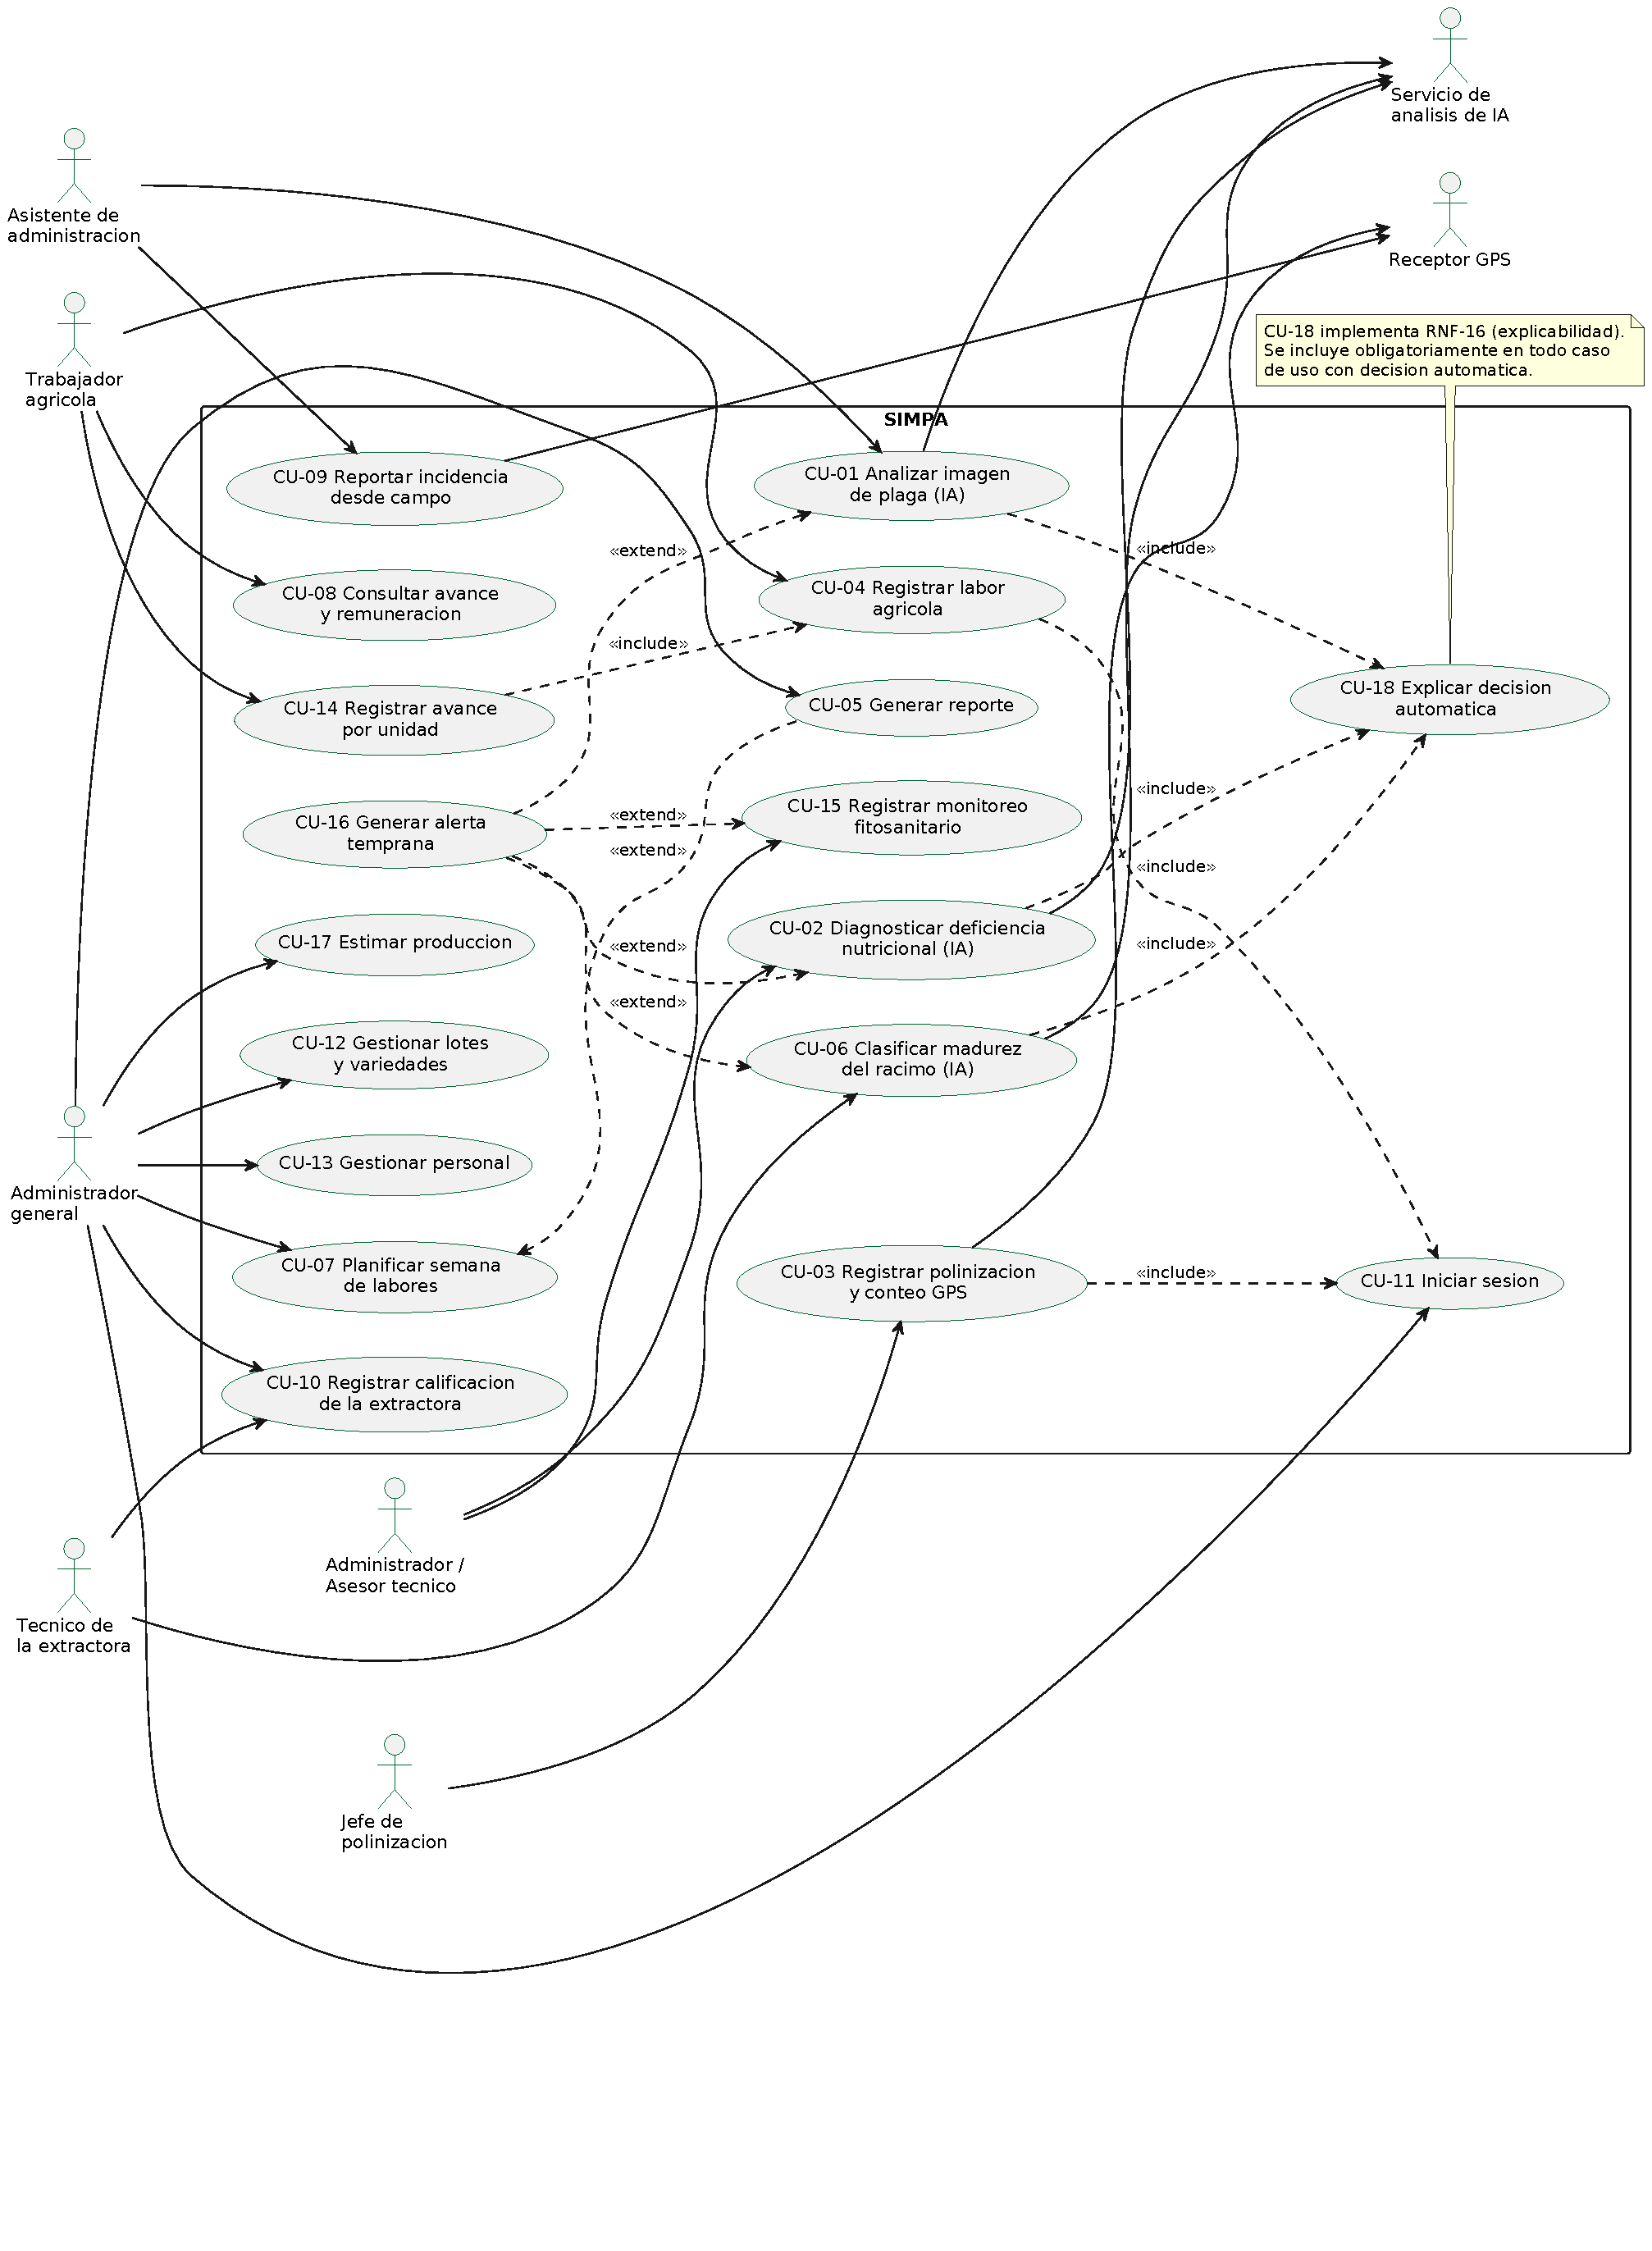
\includegraphics[width=0.91\textwidth]{img/casos_uso_general}
\caption{Diagrama general de casos de uso del SIMPA, con los ocho actores y el límite del sistema.}
\label{fig:cu_general}
\end{figure}

\noindent\textbf{Relaciones de inclusión y extensión.} \id{CU-14} incluye a \id{CU-04}, dado que el
registro de avance presupone una labor registrada. \id{CU-04} y \id{CU-03} incluyen a \id{CU-11},
por requerir sesión autenticada. Los tres casos de uso con decisión automática ---\id{CU-01},
\id{CU-02} y \id{CU-06}--- incluyen obligatoriamente a \id{CU-18}, que materializa el requisito de
explicabilidad \id{RNF-16}: no existe decisión automática sin explicación asociada. \id{CU-16}
extiende a los casos de diagnóstico y de monitoreo, puesto que la alerta se genera únicamente si el
resultado es positivo.

% ---------------------------------------------------------------------
\subsection{Especificación textual de los casos de uso}

Se especifican diez casos de uso, correspondientes a la totalidad de los requisitos funcionales de
prioridad \emph{Must}. Cada especificación incluye actores, precondiciones, postcondiciones, flujo
principal, al menos un flujo alternativo y al menos una excepción.

% --- CU-01
\begin{longtable}{|L{3.4cm}|L{12.0cm}|}
\hline
\rowcolor{grisclaro}\multicolumn{2}{|l|}{\textbf{CU-01 --- Analizar imagen para detectar plaga o enfermedad}}\\
\hline
\textbf{Requisitos} & \id{RF-07}, \id{RF-09}, \id{RF-12}, \id{RNF-16} \\ \hline
\textbf{Actores} & Primario: técnico fitosanitario / asistente de administración. Secundario: servicio de análisis de IA. \\ \hline
\textbf{Precondición} & Persona usuaria autenticada; lote seleccionado; cámara disponible. \\ \hline
\textbf{Postcondición} & El diagnóstico y su explicación quedan registrados y asociados al lote y a la fecha. \\ \hline
\textbf{Flujo principal} & 1. La persona usuaria selecciona el lote y la opción \emph{Analizar imagen}. \newline 2. Captura la fotografía de la palma o de la hoja. \newline 3. El sistema valida la calidad de la imagen. \newline 4. El sistema envía la imagen al servicio de IA con los parámetros de la variedad del lote. \newline 5. El servicio devuelve la clase de afectación, el nivel de confianza y el rasgo visual determinante. \newline 6. El sistema genera la explicación conforme a \id{RNF-16}. \newline 7. El sistema muestra el resultado, la explicación y la recomendación de control, y registra el diagnóstico. \\ \hline
\textbf{Flujo alternativo A} & \emph{Sin conectividad.} En el paso 4 el sistema almacena la imagen localmente y encola el análisis; al restablecerse la conexión lo ejecuta y notifica el resultado (\id{RNF-11}). \\ \hline
\textbf{Flujo alternativo B} & \emph{Confianza insuficiente.} Si el nivel de confianza es inferior al umbral configurado, el sistema no emite clasificación: informa que el resultado no es concluyente y sugiere repetir la captura o consultar a la asesoría técnica. \\ \hline
\textbf{Excepción E1} & Imagen de calidad insuficiente: el sistema solicita repetir la captura indicando el defecto detectado. \\ \hline
\textbf{Excepción E2} & Servicio de IA no disponible: el análisis queda en estado pendiente y la persona usuaria es notificada. \\ \hline
\textbf{Extensión} & Si el resultado es positivo, se ejecuta \id{CU-16} (generar alerta temprana). \\ \hline
\caption{CU-01 --- Analizar imagen para detectar plaga o enfermedad}
\end{longtable}

% --- CU-02
\begin{longtable}{|L{3.4cm}|L{12.0cm}|}
\hline
\rowcolor{grisclaro}\multicolumn{2}{|l|}{\textbf{CU-02 --- Diagnosticar deficiencia nutricional por imagen}}\\
\hline
\textbf{Requisitos} & \id{RF-08}, \id{RF-11}, \id{RNF-16} \\ \hline
\textbf{Actores} & Primario: administrador / asesor técnico. Secundario: servicio de análisis de IA. \\ \hline
\textbf{Precondición} & Persona usuaria autenticada; lote seleccionado con variedad asignada. \\ \hline
\textbf{Postcondición} & El diagnóstico nutricional y su recomendación quedan registrados en el historial del lote. \\ \hline
\textbf{Flujo principal} & 1. La persona usuaria selecciona \emph{Diagnóstico nutricional} y el lote. \newline 2. Captura la fotografía de la hoja. \newline 3. El sistema valida la imagen y la envía al servicio de IA. \newline 4. El servicio estima el elemento deficiente. \newline 5. El sistema genera una explicación de tipo causal, indicando qué signo foliar sustenta la estimación. \newline 6. El sistema muestra la deficiencia, la recomendación de fertilización y la explicación, y registra el diagnóstico. \\ \hline
\textbf{Flujo alternativo A} & La persona usuaria adjunta una imagen existente de la galería en lugar de capturarla. \\ \hline
\textbf{Flujo alternativo B} & \emph{Contraste con análisis de laboratorio.} Si el lote tiene un análisis de suelo o foliar registrado (\id{RF-11}), el sistema contrasta la estimación con los valores medidos y señala la discrepancia si la hubiere. \\ \hline
\textbf{Excepción E1} & Imagen no válida: el sistema solicita repetir la captura. \\ \hline
\textbf{Excepción E2} & Lote sin variedad asignada: el sistema advierte que la estimación puede no ser aplicable y solicita completar el dato. \\ \hline
\textbf{Extensión} & Si la deficiencia estimada es severa, se ejecuta \id{CU-16}. \\ \hline
\caption{CU-02 --- Diagnosticar deficiencia nutricional por imagen}
\end{longtable}

% --- CU-03
\begin{longtable}{|L{3.4cm}|L{12.0cm}|}
\hline
\rowcolor{grisclaro}\multicolumn{2}{|l|}{\textbf{CU-03 --- Registrar polinización y conteo georreferenciado}}\\
\hline
\textbf{Requisitos} & \id{RF-13}, \id{RF-14}, \id{RNF-05}, \id{RNF-12}, \id{RL-03} \\ \hline
\textbf{Actores} & Primario: polinizador. Secundario: receptor GPS. \\ \hline
\textbf{Precondición} & Lote en etapa de polinización; sesión iniciada; consentimiento de geolocalización vigente. \\ \hline
\textbf{Postcondición} & La polinización y el conteo diario quedan registrados por persona, lote y fecha, sin ingreso manual planta por planta. \\ \hline
\textbf{Flujo principal} & 1. El polinizador inicia la jornada en el lote. \newline 2. El sistema verifica la vigencia del consentimiento de geolocalización. \newline 3. El sistema activa el rastreo con período de muestreo de 30 s. \newline 4. Durante la jornada, el sistema almacena las marcaciones georreferenciadas. \newline 5. El polinizador registra el estado de la antesis y la verificación visual. \newline 6. Al cierre, el sistema calcula el número de flores polinizadas a partir de las marcaciones. \newline 7. El sistema almacena el registro y muestra el total a la persona trabajadora. \\ \hline
\textbf{Flujo alternativo A} & \emph{Consentimiento revocado.} Si el consentimiento no está vigente, el sistema no activa el rastreo y habilita el registro manual del número de flores, sin penalización para la persona trabajadora (\id{RL-03}). \\ \hline
\textbf{Flujo alternativo B} & \emph{Sin conectividad.} Las marcaciones se almacenan localmente y se sincronizan al reconectar (\id{RNF-11}). \\ \hline
\textbf{Excepción E1} & Precisión GPS superior a 10 m: el sistema conserva el dato marcándolo como de precisión degradada y advierte a la persona usuaria, sin descartar la jornada (\id{RNF-12}). \\ \hline
\textbf{Excepción E2} & Pérdida total de señal GPS durante la jornada: el sistema conserva el tramo registrado y solicita completar el conteo de forma manual para el tramo faltante. \\ \hline
\caption{CU-03 --- Registrar polinización y conteo georreferenciado}
\end{longtable}

% --- CU-04
\begin{longtable}{|L{3.4cm}|L{12.0cm}|}
\hline
\rowcolor{grisclaro}\multicolumn{2}{|l|}{\textbf{CU-04 --- Registrar labor agrícola}}\\
\hline
\textbf{Requisitos} & \id{RF-04}, \id{RF-28}, \id{RF-35} \\ \hline
\textbf{Actores} & Primario: trabajador agrícola. Alternativo: jefe de campo (registro delegado). \\ \hline
\textbf{Precondición} & Lote y persona trabajadora registrados; persona usuaria autenticada. \\ \hline
\textbf{Postcondición} & La labor y su avance quedan en el historial del lote y computan para el cumplimiento del plan semanal. \\ \hline
\textbf{Flujo principal} & 1. La persona usuaria selecciona el lote y el tipo de labor. \newline 2. Ingresa la cantidad ejecutada en la unidad correspondiente. \newline 3. El sistema valida que la unidad corresponda al tipo de labor. \newline 4. El sistema registra la labor asociada al lote, la fecha y la persona responsable. \newline 5. El sistema actualiza el avance acumulado del período y el cumplimiento de la meta semanal. \\ \hline
\textbf{Flujo alternativo A} & \emph{Registro delegado.} Si la persona trabajadora no dispone de dispositivo propio, el jefe de campo registra el avance en su nombre; el sistema conserva en bitácora la identidad de quien efectuó el registro (\id{RF-35}, \id{RD-10}). \\ \hline
\textbf{Flujo alternativo B} & \emph{Sin conectividad.} La labor se almacena localmente y se sincroniza al reconectar. \\ \hline
\textbf{Excepción E1} & Datos incompletos: el sistema impide guardar y señala los campos faltantes. \\ \hline
\textbf{Excepción E2} & Unidad incompatible con el tipo de labor: el sistema rechaza el registro e indica la unidad esperada. \\ \hline
\caption{CU-04 --- Registrar labor agrícola}
\end{longtable}

% --- CU-05
\begin{longtable}{|L{3.4cm}|L{12.0cm}|}
\hline
\rowcolor{grisclaro}\multicolumn{2}{|l|}{\textbf{CU-05 --- Generar reporte}}\\
\hline
\textbf{Requisitos} & \id{RF-19}, \id{RF-26} \\ \hline
\textbf{Actores} & Primario: administrador general. \\ \hline
\textbf{Precondición} & Existen registros en el período seleccionado. \\ \hline
\textbf{Postcondición} & El reporte queda disponible para consulta o exportación. \\ \hline
\textbf{Flujo principal} & 1. La persona administradora selecciona el tipo de reporte y el período. \newline 2. El sistema consolida labores, avance, producción y alertas del período. \newline 3. El sistema genera y presenta el reporte. \newline 4. La persona administradora lo consulta o lo exporta a PDF o a hoja de cálculo. \\ \hline
\textbf{Flujo alternativo A} & Filtrado por lote, por equipo o por persona trabajadora. \\ \hline
\textbf{Flujo alternativo B} & \emph{Reporte de cumplimiento semanal.} El sistema contrasta el plan de la semana con lo ejecutado y destaca las metas no alcanzadas y su remanente. \\ \hline
\textbf{Excepción E1} & Sin registros en el período: el sistema informa la ausencia de datos y propone un período alternativo con información disponible. \\ \hline
\caption{CU-05 --- Generar reporte}
\end{longtable}

% --- CU-06
\begin{longtable}{|L{3.4cm}|L{12.0cm}|}
\hline
\rowcolor{grisclaro}\multicolumn{2}{|l|}{\textbf{CU-06 --- Clasificar la madurez del racimo}}\\
\hline
\textbf{Requisitos} & \id{RF-21}, \id{RF-22}, \id{RD-07}, \id{RD-08}, \id{RNF-01}, \id{RNF-16} \\ \hline
\textbf{Actores} & Primario: cosechador / técnico de la extractora. Secundario: servicio de análisis de IA. \\ \hline
\textbf{Precondición} & Lote con variedad asignada; persona usuaria autenticada. \\ \hline
\textbf{Postcondición} & La clasificación queda asociada al racimo, al lote y a la fecha, y actualiza el porcentaje estimado de fruta verde del lote. \\ \hline
\textbf{Flujo principal} & 1. La persona usuaria selecciona el lote y la opción \emph{Clasificar racimo}. \newline 2. El sistema recupera el umbral de desprendimiento de la variedad del lote. \newline 3. La persona usuaria captura la fotografía de la parte basal del racimo. \newline 4. El servicio de IA cuenta los frutos desprendidos, sin emplear el color como criterio (\id{RD-07}). \newline 5. El sistema compara el conteo con el umbral de la variedad y determina el estado. \newline 6. El sistema genera una explicación por contraste, indicando el conteo obtenido y el umbral aplicable. \newline 7. El sistema registra la clasificación y actualiza el porcentaje de fruta verde del lote. \\ \hline
\textbf{Flujo alternativo A} & \emph{Verificación previa al despacho.} La persona usuaria solicita el porcentaje estimado de fruta verde del lote; si alcanza o supera el umbral de penalización, el sistema emite alerta preventiva y desaconseja el despacho (\id{RF-22}). \\ \hline
\textbf{Flujo alternativo B} & \emph{Sobremadurez.} Si el conteo excede ampliamente el umbral, el sistema clasifica el racimo como sobremaduro y advierte sobre el incremento de acidez. \\ \hline
\textbf{Excepción E1} & Lote sin variedad asignada: el sistema no clasifica y solicita completar el dato, dado que el umbral depende de la variedad. \\ \hline
\textbf{Excepción E2} & Parte basal no visible en la imagen: el sistema solicita repetir la captura indicando el encuadre requerido. \\ \hline
\caption{CU-06 --- Clasificar la madurez del racimo}
\end{longtable}

% --- CU-07
\begin{longtable}{|L{3.4cm}|L{12.0cm}|}
\hline
\rowcolor{grisclaro}\multicolumn{2}{|l|}{\textbf{CU-07 --- Planificar la semana de labores}}\\
\hline
\textbf{Requisitos} & \id{RF-26}, \id{RF-27}, \id{RF-34}, \id{RF-37} a \id{RF-39} \\ \hline
\textbf{Actores} & Primario: administrador general. \\ \hline
\textbf{Precondición} & Lotes y tipos de labor registrados. \\ \hline
\textbf{Postcondición} & El plan de la semana queda publicado y disponible para el seguimiento diario. \\ \hline
\textbf{Flujo principal} & 1. La persona administradora crea el plan de la semana. \newline 2. Para cada lote, define las labores previstas con su meta y unidad. \newline 3. El sistema incorpora automáticamente los remanentes arrastrados de la semana anterior. \newline 4. La persona administradora registra los insumos requeridos. \newline 5. El sistema publica el plan y lo hace visible al jefe de campo. \\ \hline
\textbf{Flujo alternativo A} & \emph{Cierre de semana.} Al cierre, el sistema calcula el cumplimiento de cada meta; si es parcial, genera el remanente como labor pendiente de la semana siguiente, vinculada a la de origen (\id{RF-27}). \\ \hline
\textbf{Flujo alternativo B} & Ajuste del plan durante la semana en curso, conservando la versión previa en bitácora. \\ \hline
\textbf{Flujo alternativo C} & \emph{Liquidación y aprobación.} Al cierre, el sistema genera la liquidación que contrasta cantidad presupuestada, cantidad ejecutada, tarifa y valor por grupo de labor, totaliza el gasto presupuestado frente al real, e incorpora las labores no presupuestadas en su grupo diferenciado (\id{RF-37}, \id{RF-38}). La persona administradora aprueba la liquidación y el período queda cerrado (\id{RF-39}). \\ \hline
\textbf{Excepción E1} & Meta expresada en unidad incompatible con el tipo de labor: el sistema rechaza la meta e indica la unidad esperada. \\ \hline
\textbf{Excepción E2} & Existe un plan publicado para la misma semana: el sistema advierte y solicita confirmación antes de sustituirlo. \\ \hline
\caption{CU-07 --- Planificar la semana de labores}
\end{longtable}

% --- CU-08
\begin{longtable}{|L{3.4cm}|L{12.0cm}|}
\hline
\rowcolor{grisclaro}\multicolumn{2}{|l|}{\textbf{CU-08 --- Consultar avance acumulado y remuneración estimada}}\\
\hline
\textbf{Requisitos} & \id{RF-29}, \id{RF-36}, \id{RL-04} \\ \hline
\textbf{Actores} & Primario: trabajador agrícola. \\ \hline
\textbf{Precondición} & Existen registros de avance de la persona trabajadora en el período. \\ \hline
\textbf{Postcondición} & Se presenta el consolidado del período, sin posibilidad de edición por parte de la persona trabajadora. \\ \hline
\textbf{Flujo principal} & 1. La persona trabajadora accede a \emph{Mi avance}. \newline 2. Selecciona el período (quincena en curso por defecto). \newline 3. El sistema agrega sus registros de avance por tipo de labor. \newline 4. El sistema obtiene del catálogo la tarifa vigente de cada tipo de labor a la fecha de cada registro y calcula la remuneración estimada correspondiente al trabajo por avance. \newline 5. El sistema presenta el desglose por labor y el total estimado. \\ \hline
\textbf{Flujo alternativo A} & \emph{Ejercicio del derecho de acceso.} La persona trabajadora solicita la exportación de sus datos personales; el sistema genera el archivo conforme al Art. 12 de la LOPDP (\id{RL-04}). \\ \hline
\textbf{Flujo alternativo B} & \emph{Discrepancia.} La persona trabajadora marca un registro como discrepante; el sistema notifica a la administración sin modificar el dato original, y la corrección se tramita mediante \id{RL-05}. \\ \hline
\textbf{Excepción E1} & Sin registros en el período: el sistema informa la ausencia de datos. \\ \hline
\textbf{Excepción E2} & La labor carece de tarifa vigente en el catálogo (\id{RF-36}) a la fecha del registro: el sistema muestra el avance en unidades, omite la estimación monetaria e indica que la tarifa no está vigente para esa fecha. \\ \hline
\caption{CU-08 --- Consultar avance acumulado y remuneración estimada}
\end{longtable}

% --- CU-09
\begin{longtable}{|L{3.4cm}|L{12.0cm}|}
\hline
\rowcolor{grisclaro}\multicolumn{2}{|l|}{\textbf{CU-09 --- Reportar incidencia desde el campo}}\\
\hline
\textbf{Requisitos} & \id{RF-30}, \id{RF-31}, \id{RF-12} \\ \hline
\textbf{Actores} & Primario: asistente de administración / trabajador agrícola. Secundario: receptor GPS. \\ \hline
\textbf{Precondición} & Persona usuaria autenticada; cámara y GPS disponibles. \\ \hline
\textbf{Postcondición} & La incidencia queda registrada con fotografía y coordenadas, e incorporada a la lista de pendientes de verificación. \\ \hline
\textbf{Flujo principal} & 1. La persona usuaria selecciona \emph{Reportar incidencia}. \newline 2. Captura la fotografía de la afectación. \newline 3. El sistema obtiene las coordenadas del punto. \newline 4. La persona usuaria selecciona el lote y describe la afectación. \newline 5. El sistema registra la incidencia georreferenciada. \newline 6. El sistema la incorpora a la lista de pendientes de la persona supervisora. \\ \hline
\textbf{Flujo alternativo A} & \emph{Análisis asistido.} La persona usuaria solicita el análisis de la fotografía; se ejecuta \id{CU-01} y el diagnóstico se asocia a la incidencia. \\ \hline
\textbf{Flujo alternativo B} & \emph{Verificación en visita.} La persona supervisora recorre su lista de pendientes, ubica la incidencia por sus coordenadas y la marca como verificada o descartada. \\ \hline
\textbf{Excepción E1} & GPS no disponible: el sistema registra la incidencia solicitando la selección manual del lote y la marca como de ubicación aproximada. \\ \hline
\textbf{Excepción E2} & Sin conectividad: la incidencia se encola y se sincroniza al reconectar, conservando el instante original de captura. \\ \hline
\caption{CU-09 --- Reportar incidencia desde el campo}
\end{longtable}

% --- CU-10
\begin{longtable}{|L{3.4cm}|L{12.0cm}|}
\hline
\rowcolor{grisclaro}\multicolumn{2}{|l|}{\textbf{CU-10 --- Registrar la calificación de la planta extractora}}\\
\hline
\textbf{Requisitos} & \id{RF-23}, \id{RF-24}, \id{RF-25}, \id{RF-33} \\ \hline
\textbf{Actores} & Primario: administrador general. \\ \hline
\textbf{Precondición} & Existe un despacho registrado con su fecha de corte. \\ \hline
\textbf{Postcondición} & La calificación queda asociada al lote de origen y disponible para el análisis de trazabilidad. \\ \hline
\textbf{Flujo principal} & 1. La persona administradora selecciona el despacho. \newline 2. Ingresa los datos del ticket de pesaje: peso bruto, tara y neto. \newline 3. Ingresa la calificación de calidad: tamaño del fruto, porcentaje de fruta verde, sobremadura, malformación y pedúnculo largo. \newline 4. El sistema calcula el intervalo entre el corte y la entrega. \newline 5. El sistema registra la calificación y la asocia al lote de origen. \\ \hline
\textbf{Flujo alternativo A} & \emph{Análisis de trazabilidad.} Ante una calificación desfavorable, la persona administradora consulta la cadena lote $\rightarrow$ fecha de corte $\rightarrow$ cuadrilla, y contrasta con las labores del período para distinguir si el origen está en la cosecha o en el manejo del cultivo (\id{RF-24}). \\ \hline
\textbf{Flujo alternativo B} & \emph{Ausencia de guía de remisión.} Si el despacho se registra sin número de guía, el sistema advierte antes del cierre (\id{RF-33}). \\ \hline
\textbf{Excepción E1} & El intervalo entre corte y entrega supera el valor recomendado para la variedad: el sistema registra la advertencia junto al despacho (\id{RF-25}). \\ \hline
\textbf{Excepción E2} & La suma de pesos es inconsistente (neto distinto de bruto menos tara): el sistema rechaza el registro e indica la inconsistencia. \\ \hline
\caption{CU-10 --- Registrar la calificación de la planta extractora}
\end{longtable}

% ---------------------------------------------------------------------
\subsection{Diagrama de clases refinado}

El modelo del dominio comprende veinticinco clases con atributos y operaciones. Incorpora tres
jerarquías de herencia (\id{Persona}--\id{Usuario} y la especialización de \id{Diagnostico} en sus
tres variantes), cuatro relaciones de composición y asociaciones con multiplicidad explícita. No
corresponde a un diseño de base de datos, sino al modelo conceptual del dominio del problema.

\begin{figure}[!htbp]
\centering
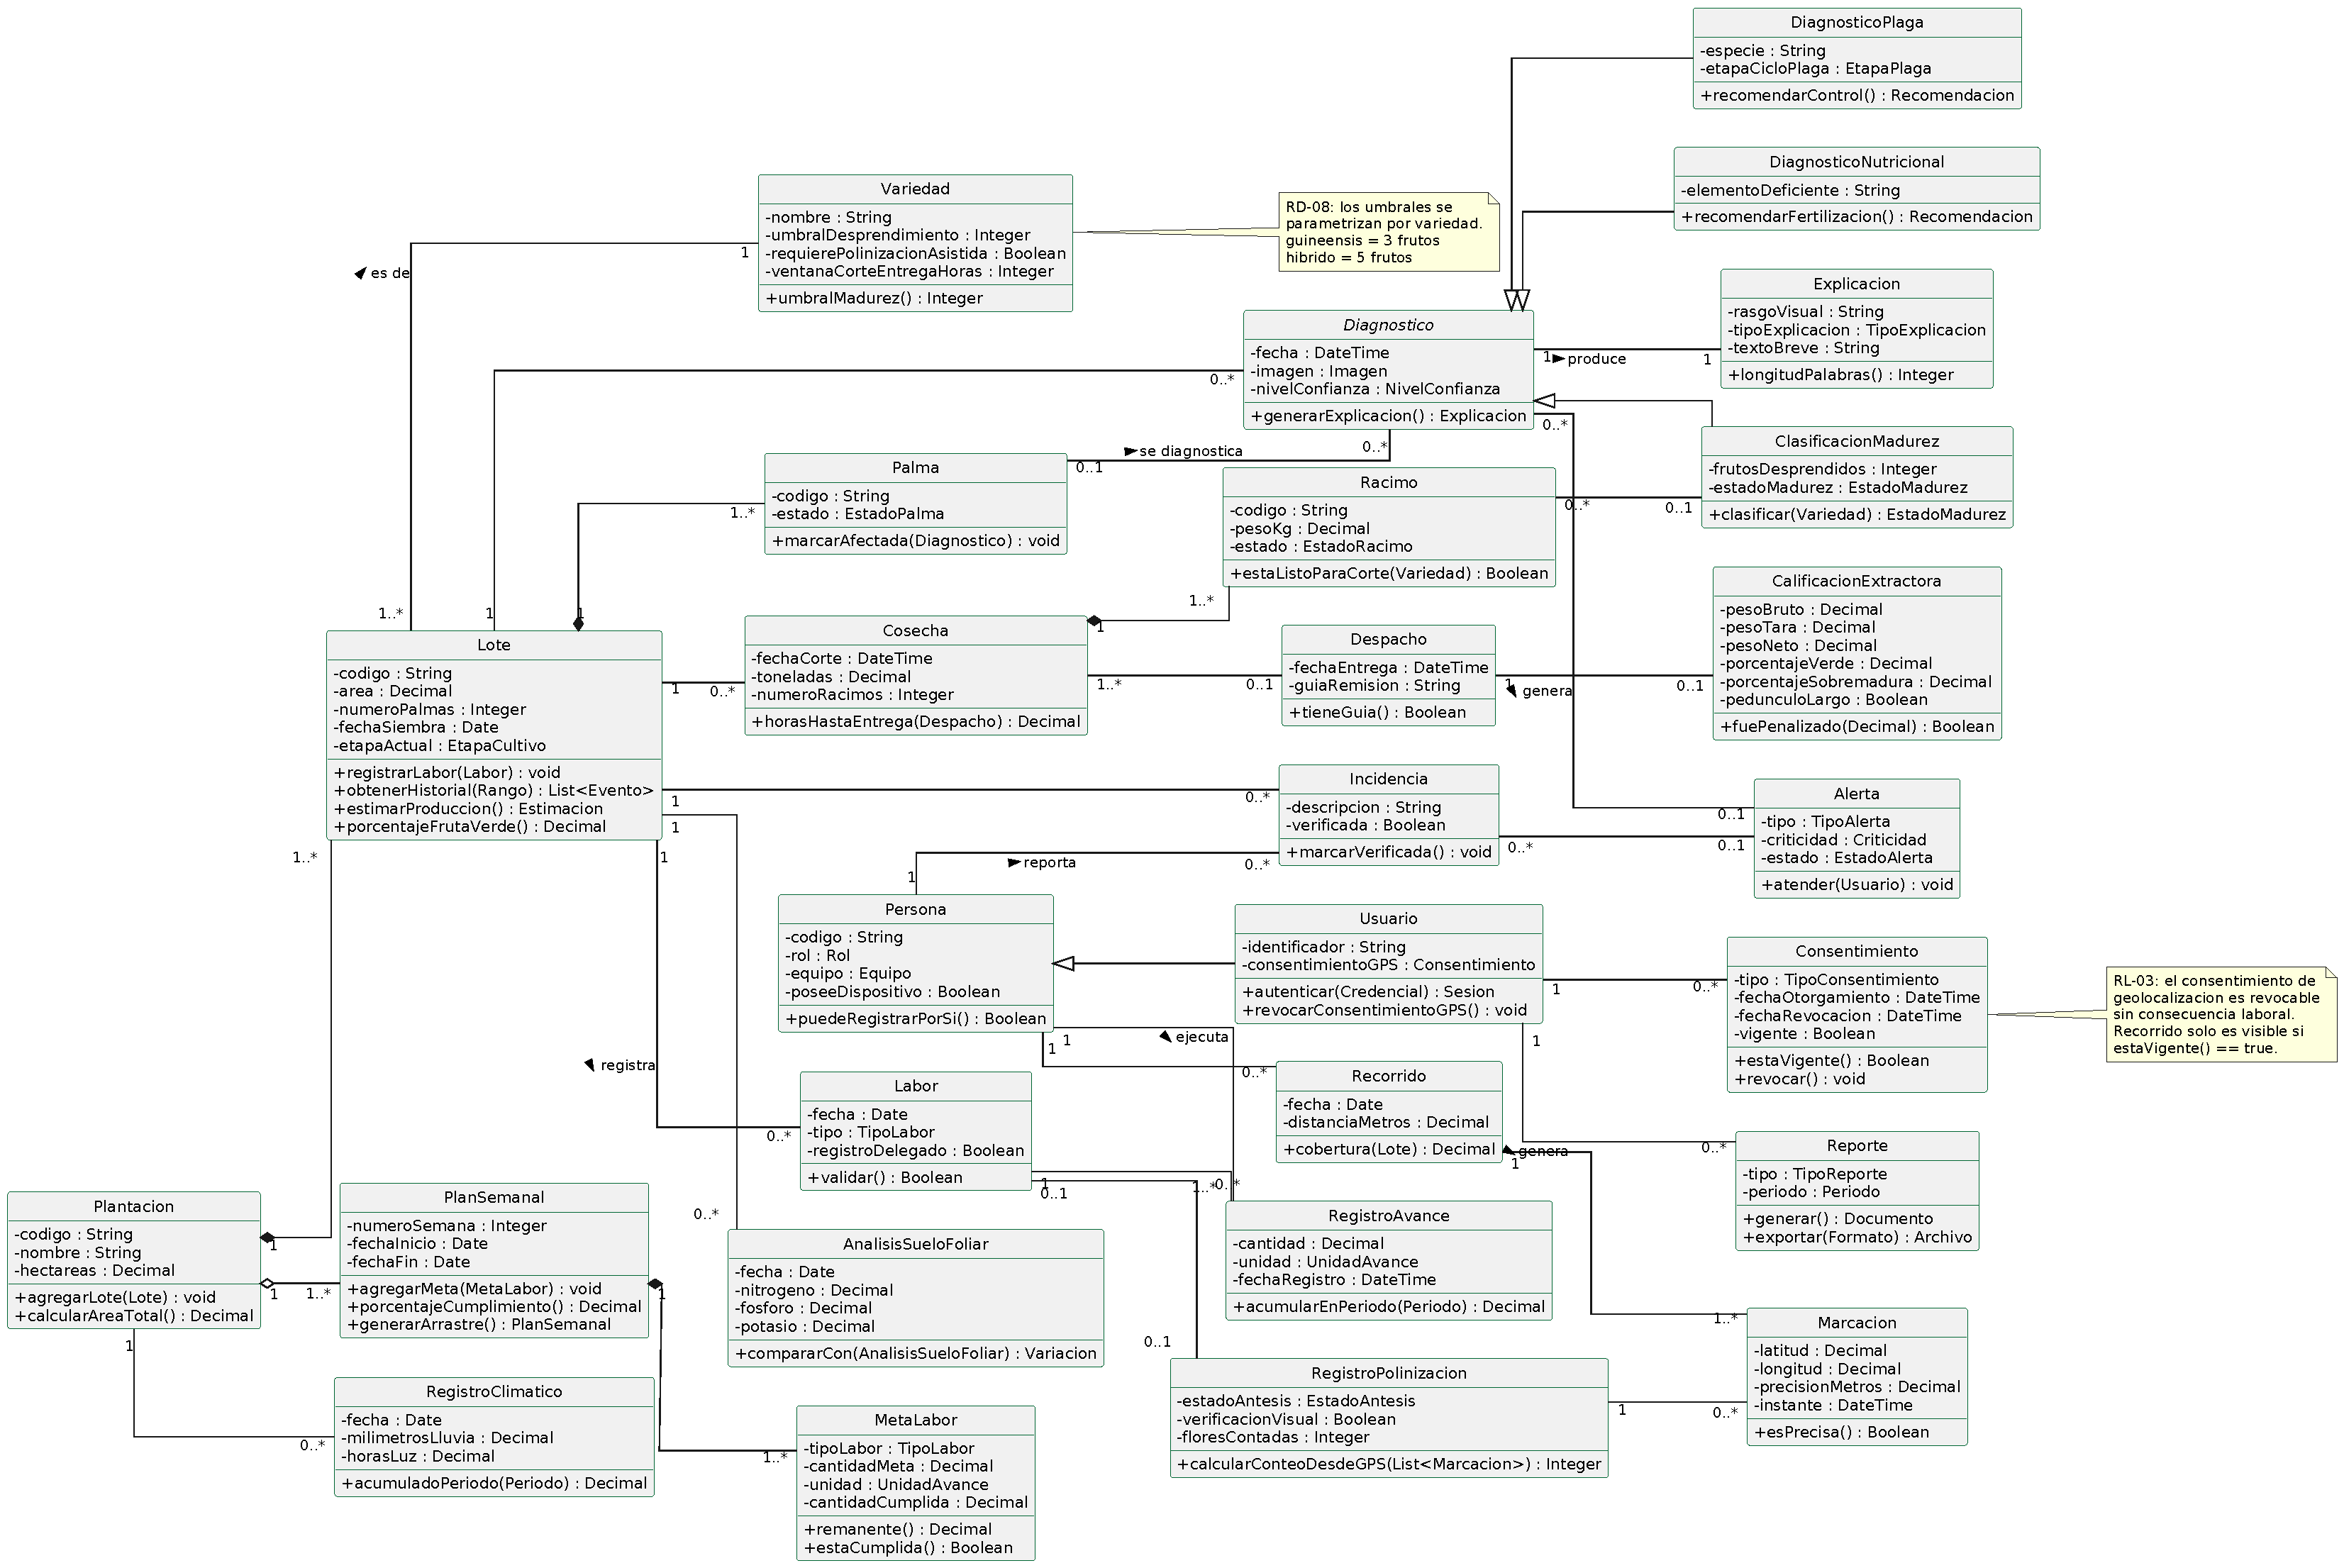
\includegraphics[width=1.0\textwidth]{img/clases_refinado}
\caption{Diagrama de clases refinado del SIMPA, con atributos y operaciones.}
\label{fig:clases}
\end{figure}

\noindent\textbf{Decisiones de modelado relevantes.} La clase \id{Consentimiento} se modela como
entidad de primer orden y no como atributo booleano de \id{Usuario}, porque el Art. 7 de la LOPDP
exige que el consentimiento sea específico por finalidad y revocable, lo que obliga a conservar su
historia. La clase \id{Variedad} concentra los umbrales de decisión ---desprendimiento, ventana
corte-entrega y necesidad de polinización asistida--- en lugar de fijarlos en la lógica de los
módulos de IA, conforme a \id{RD-08}. La clase \id{Explicacion} se asocia de forma obligatoria a
\id{Diagnostico} con multiplicidad 1:1, de modo que el modelo impide estructuralmente la existencia
de una decisión automática sin explicación (\id{RNF-16}). La clase \id{RegistroAvance} se separa de
\id{Labor} porque una labor puede acumular avances de varias personas y días, patrón observado en
los documentos de planificación semanal (\id{EV-11}).

% ---------------------------------------------------------------------
\subsection{Diagramas de secuencia}

Se presentan los diagramas de secuencia de los tres casos de uso \emph{Must} de mayor complejidad
de interacción.

\begin{figure}[!htbp]
\centering
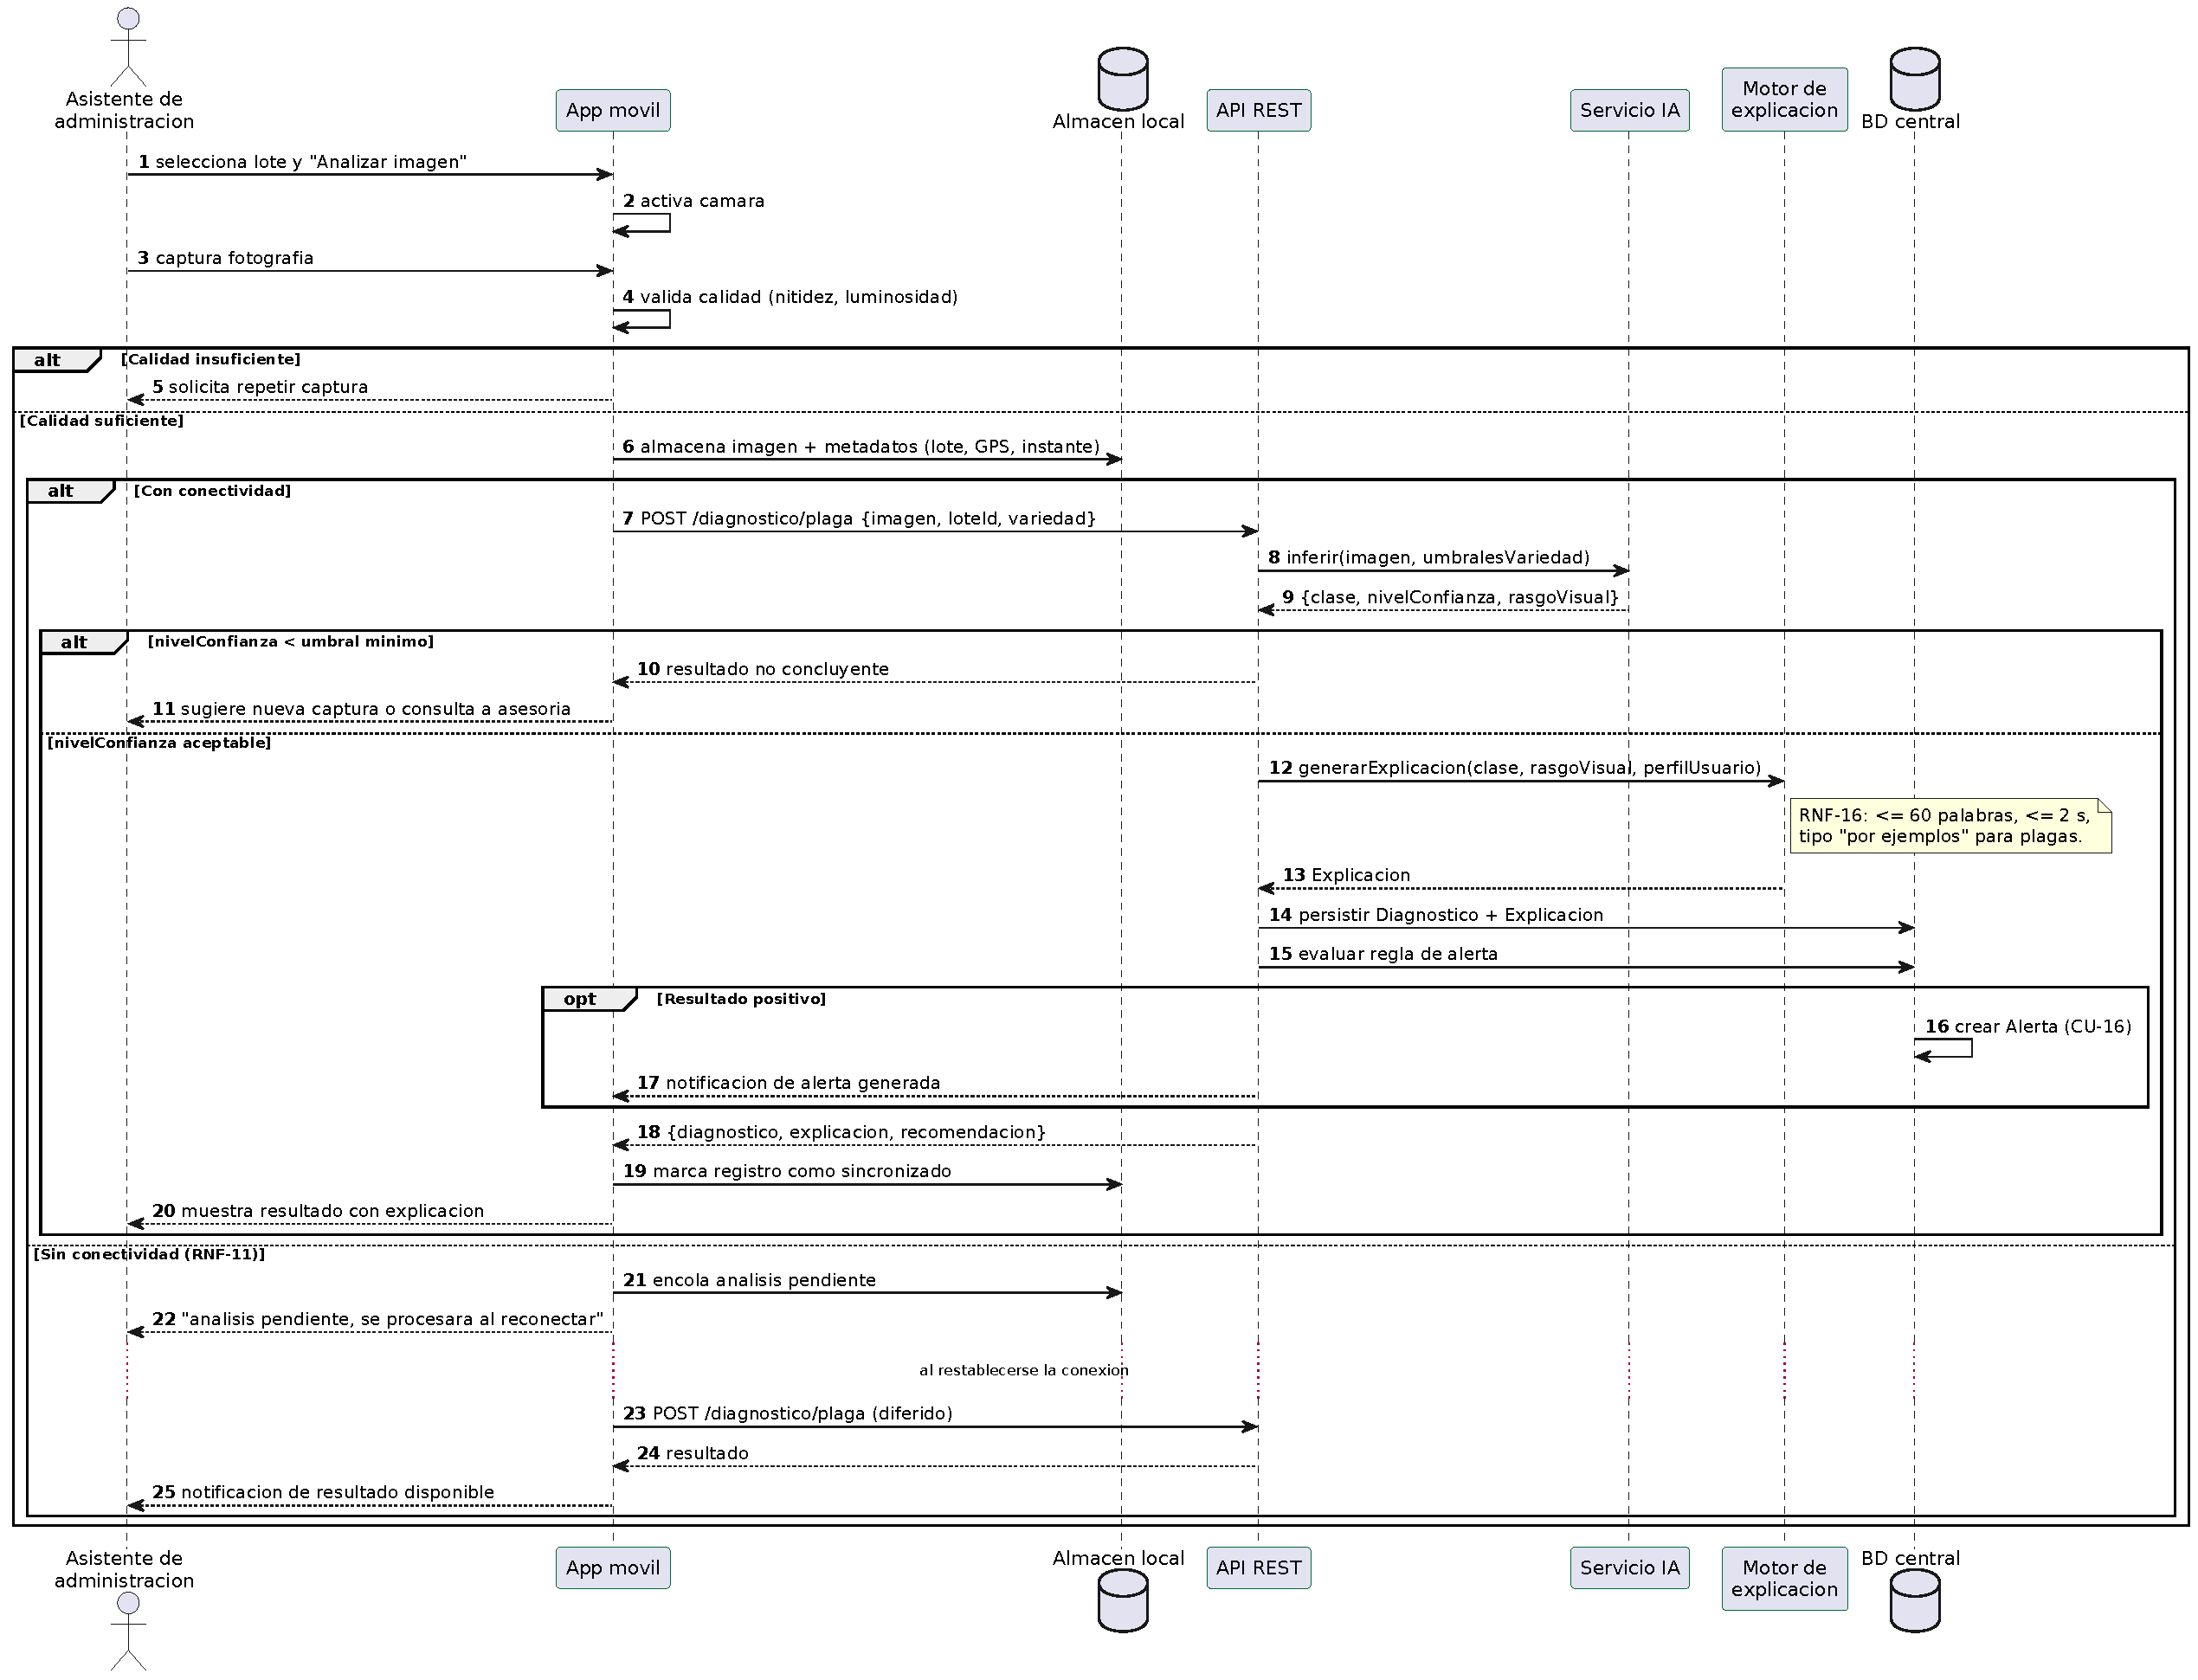
\includegraphics[width=1.0\textwidth]{img/secuencia_CU01}
\caption{Diagrama de secuencia del CU-01: análisis de imagen para detección de plaga, con las ramas de baja confianza y de operación sin conectividad.}
\label{fig:seq01}
\end{figure}

\begin{figure}[!htbp]
\centering
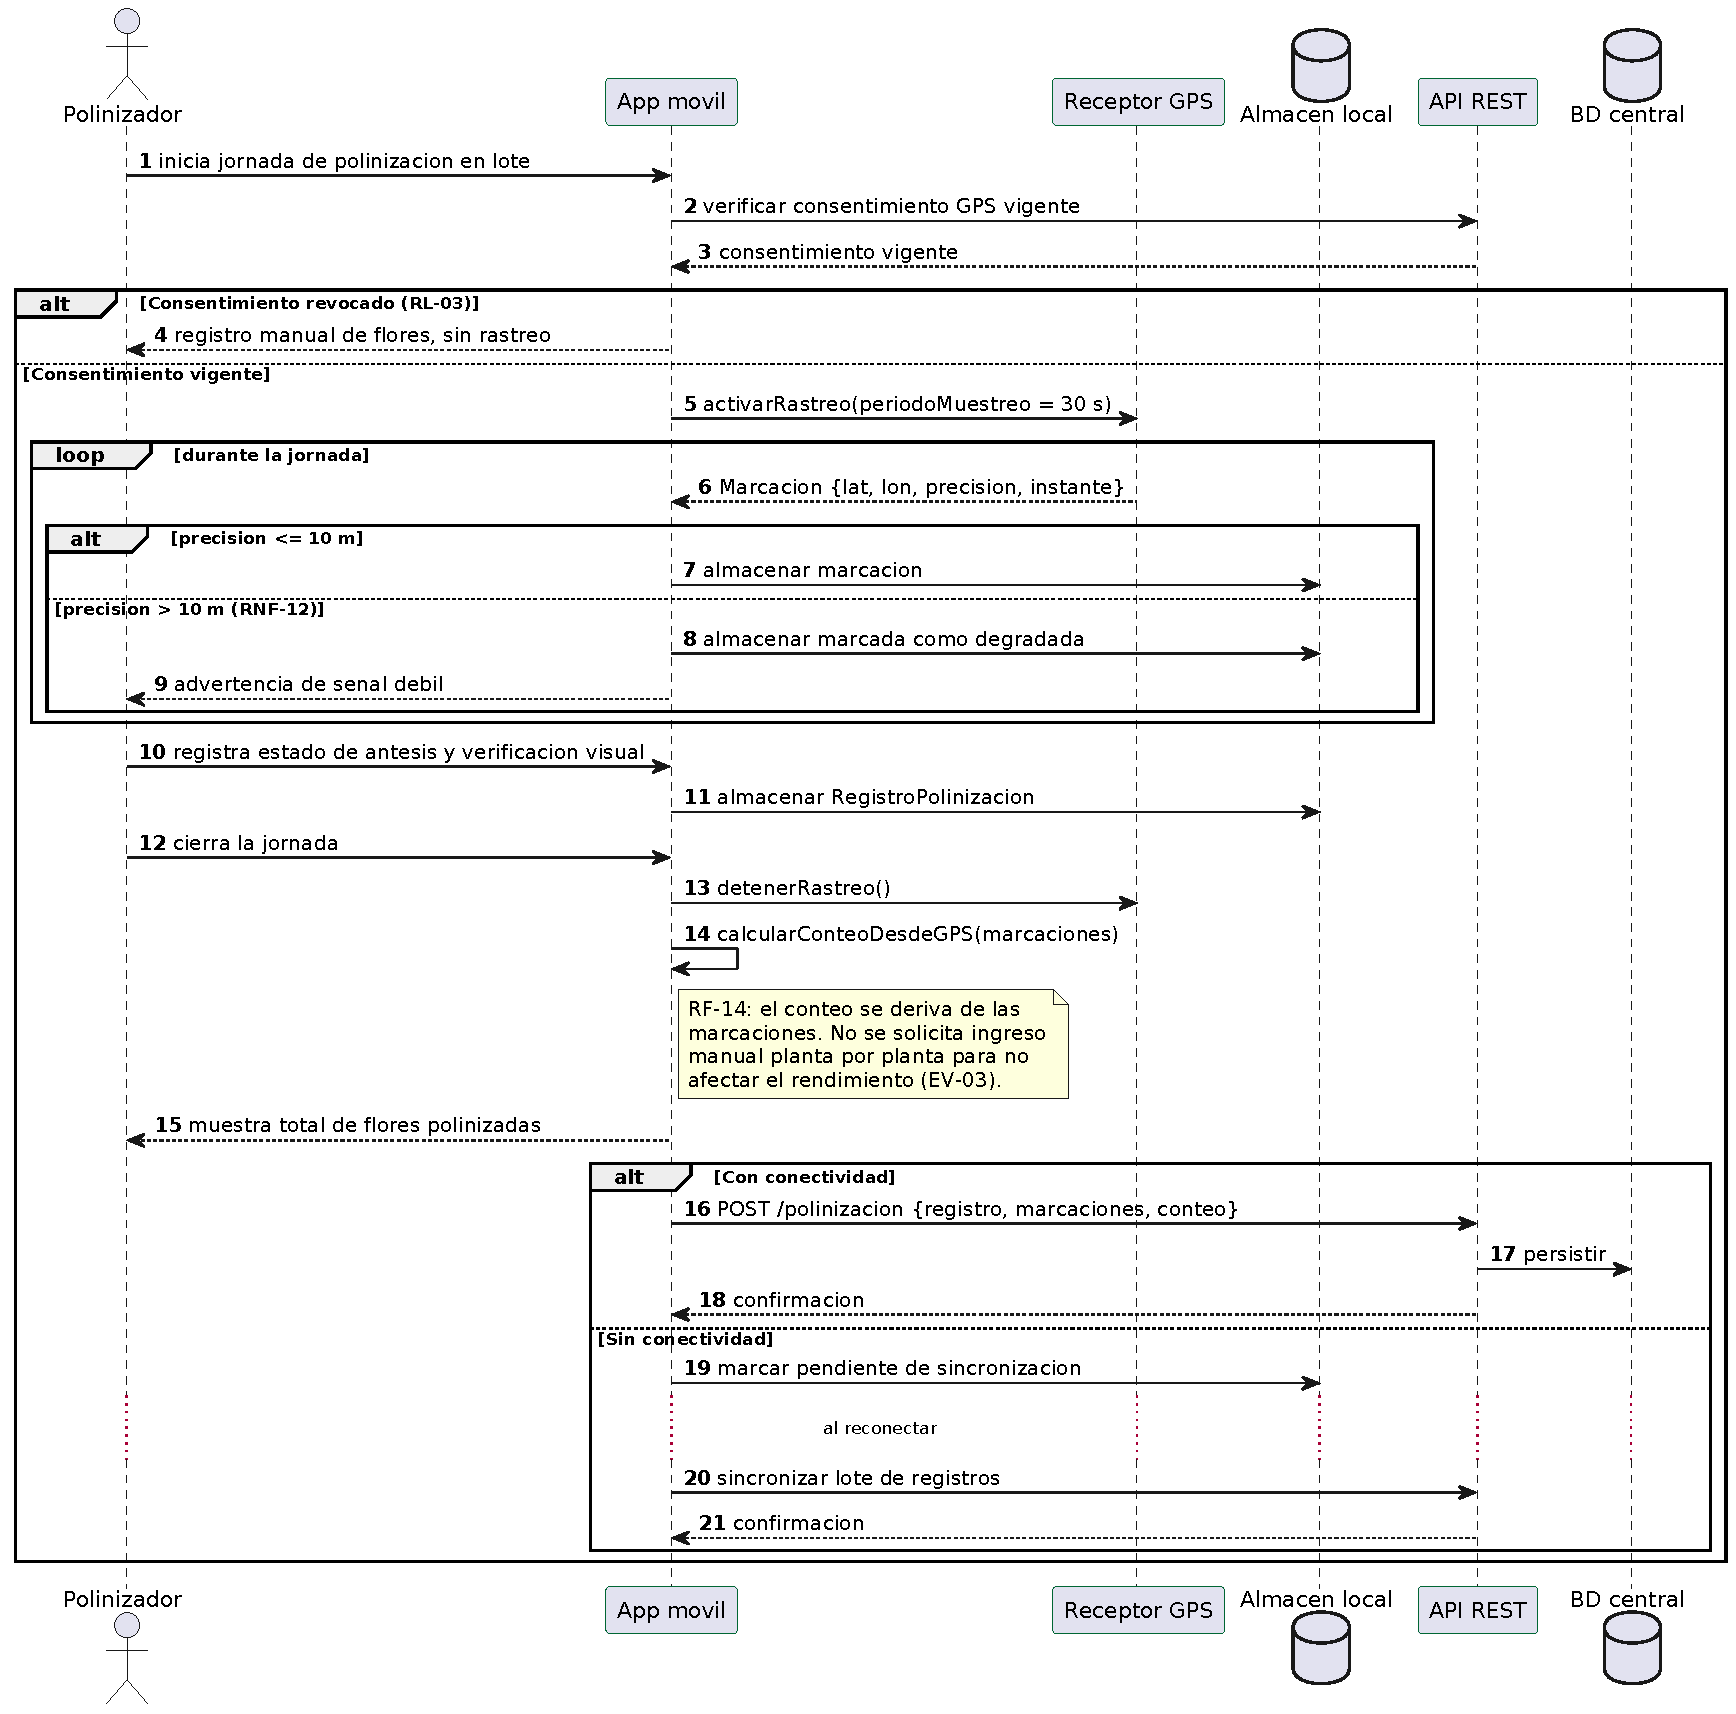
\includegraphics[width=1.0\textwidth]{img/secuencia_CU03}
\caption{Diagrama de secuencia del CU-03: registro de polinización y conteo georreferenciado, con verificación de consentimiento y manejo de precisión degradada.}
\label{fig:seq03}
\end{figure}

\begin{figure}[!htbp]
\centering
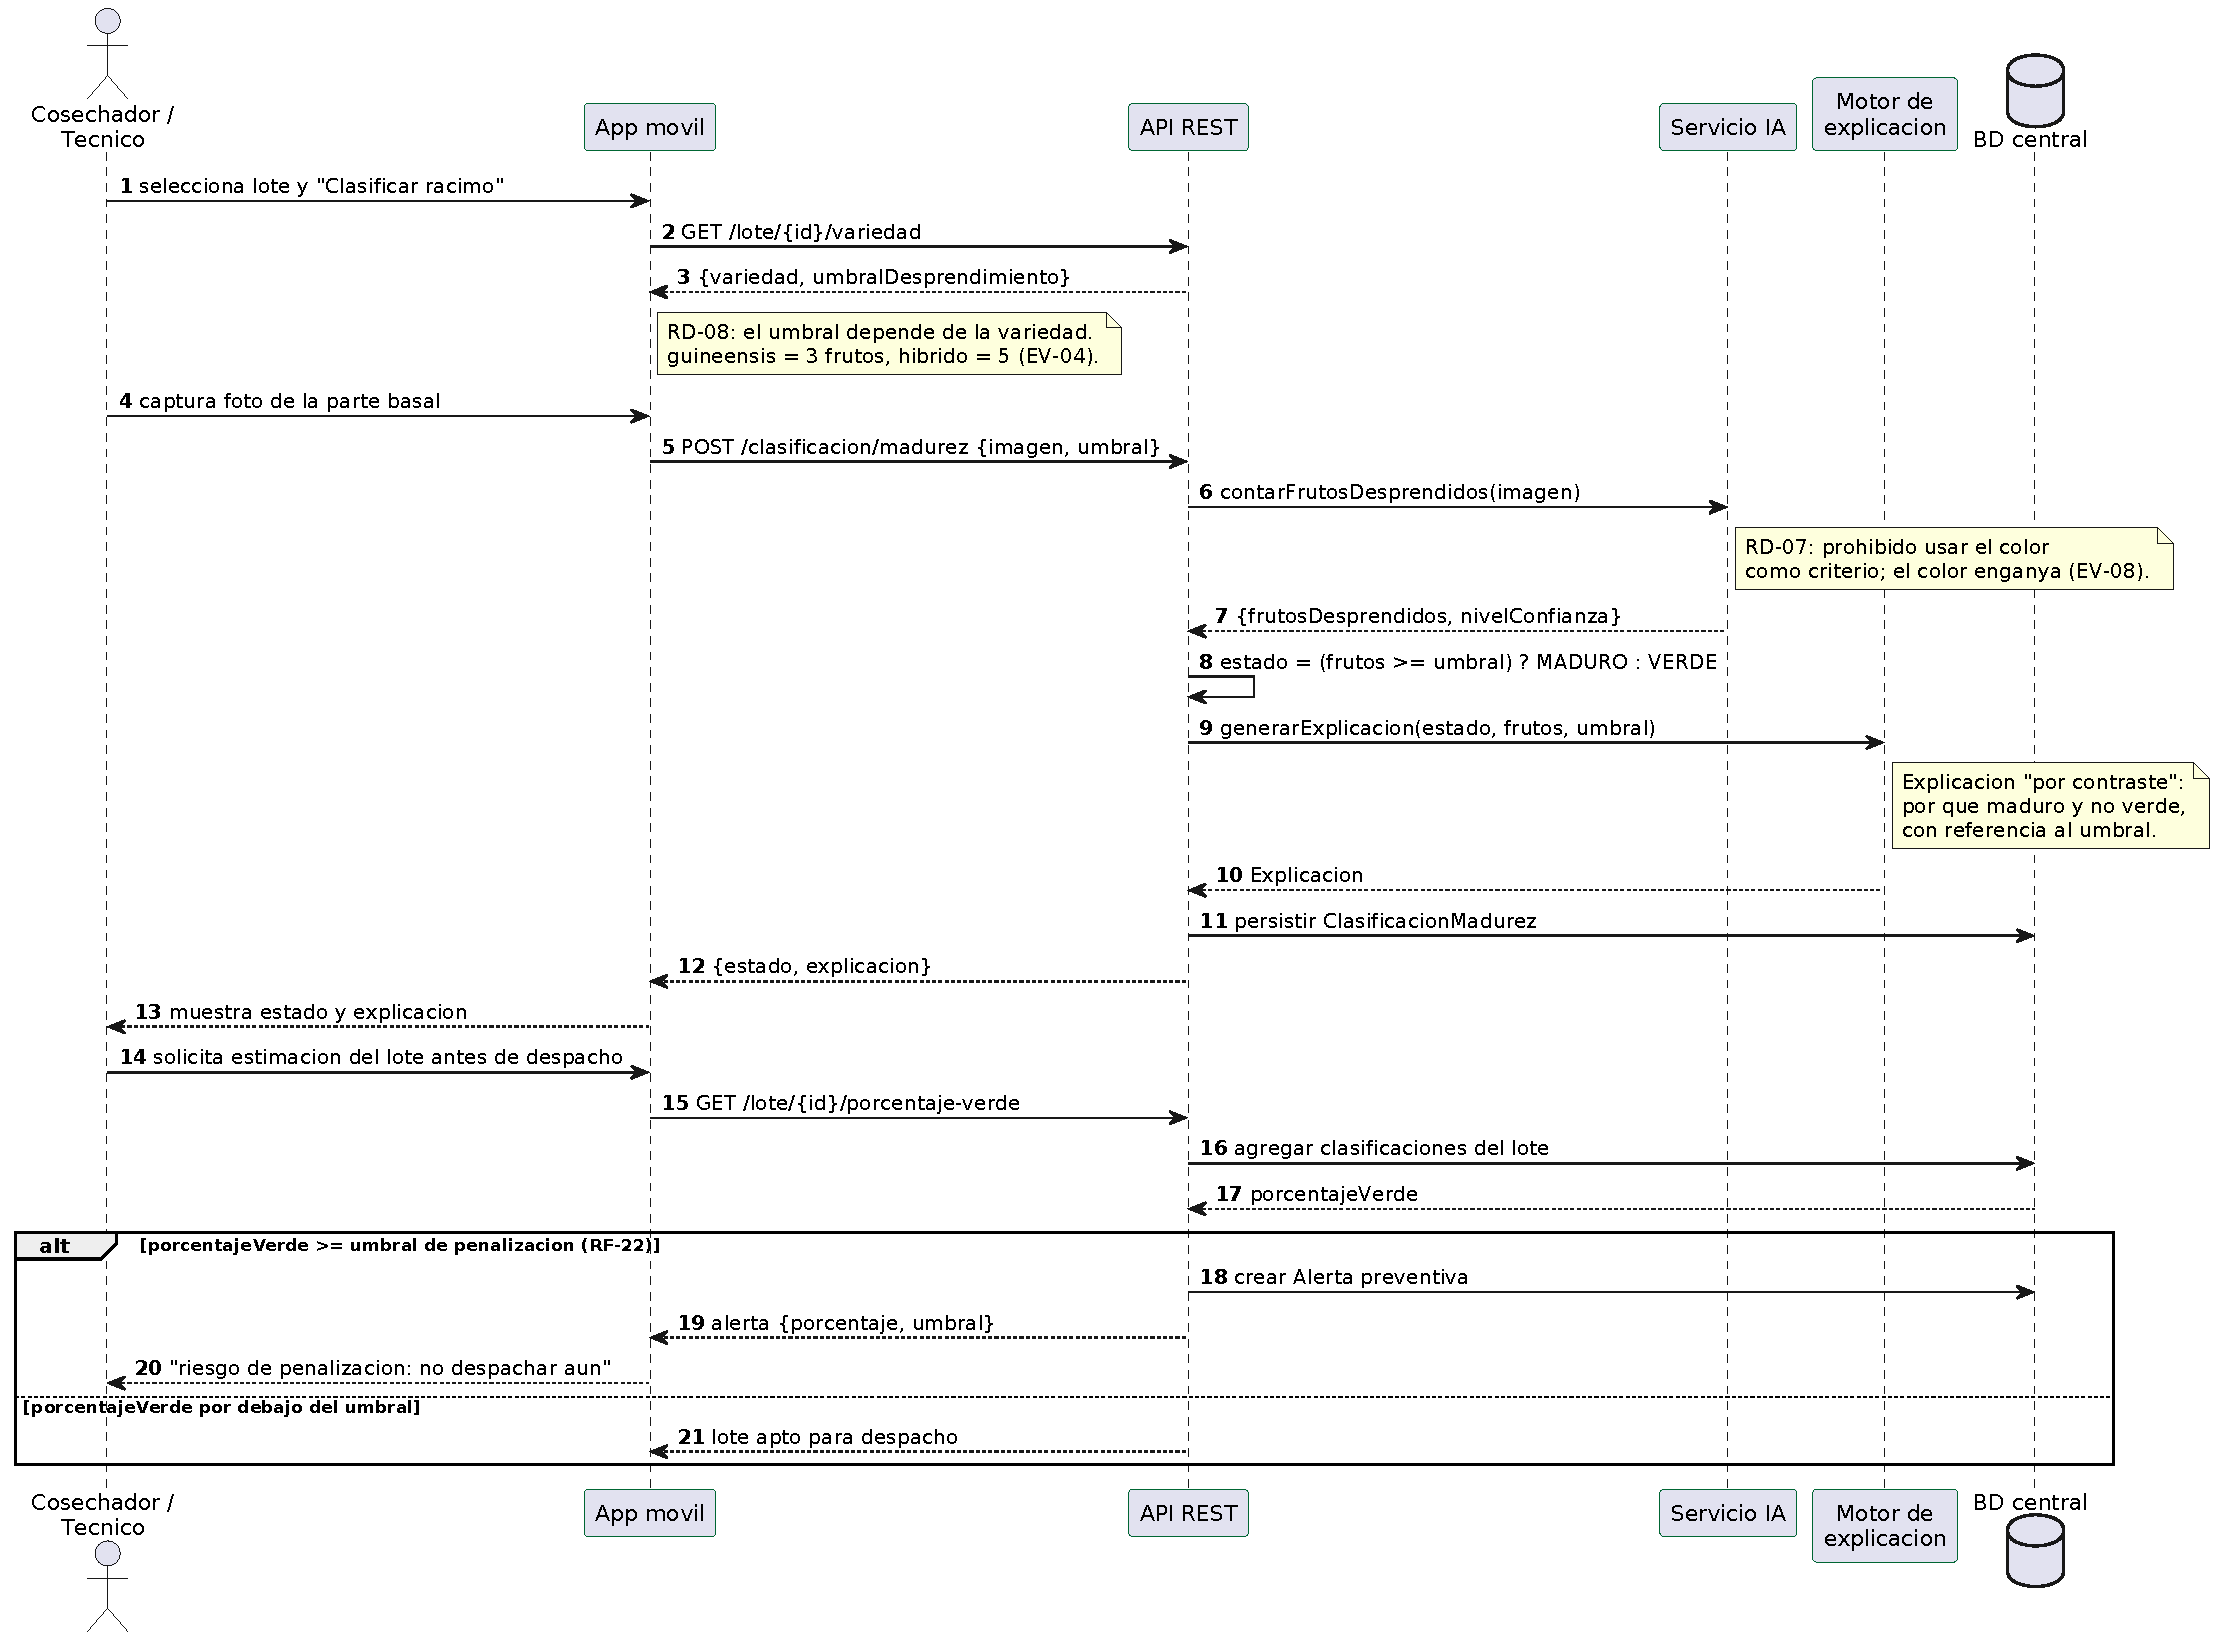
\includegraphics[width=1.0\textwidth]{img/secuencia_CU06}
\caption{Diagrama de secuencia del CU-06: clasificación de madurez del racimo y alerta preventiva de porcentaje de fruta verde.}
\label{fig:seq06}
\end{figure}

% ---------------------------------------------------------------------
\subsection{Diagrama de actividad}

El diagrama modela el ciclo semanal completo de planificación y ejecución, que constituye el proceso
central de la organización según los documentos operativos (\id{EV-11}). Incorpora la bifurcación
por disponibilidad de dispositivo (\id{RF-35}), la bifurcación por conectividad (\id{RNF-11}) y el
mecanismo de arrastre de labor incompleta (\id{RF-27}).

\begin{figure}[!htbp]
\centering
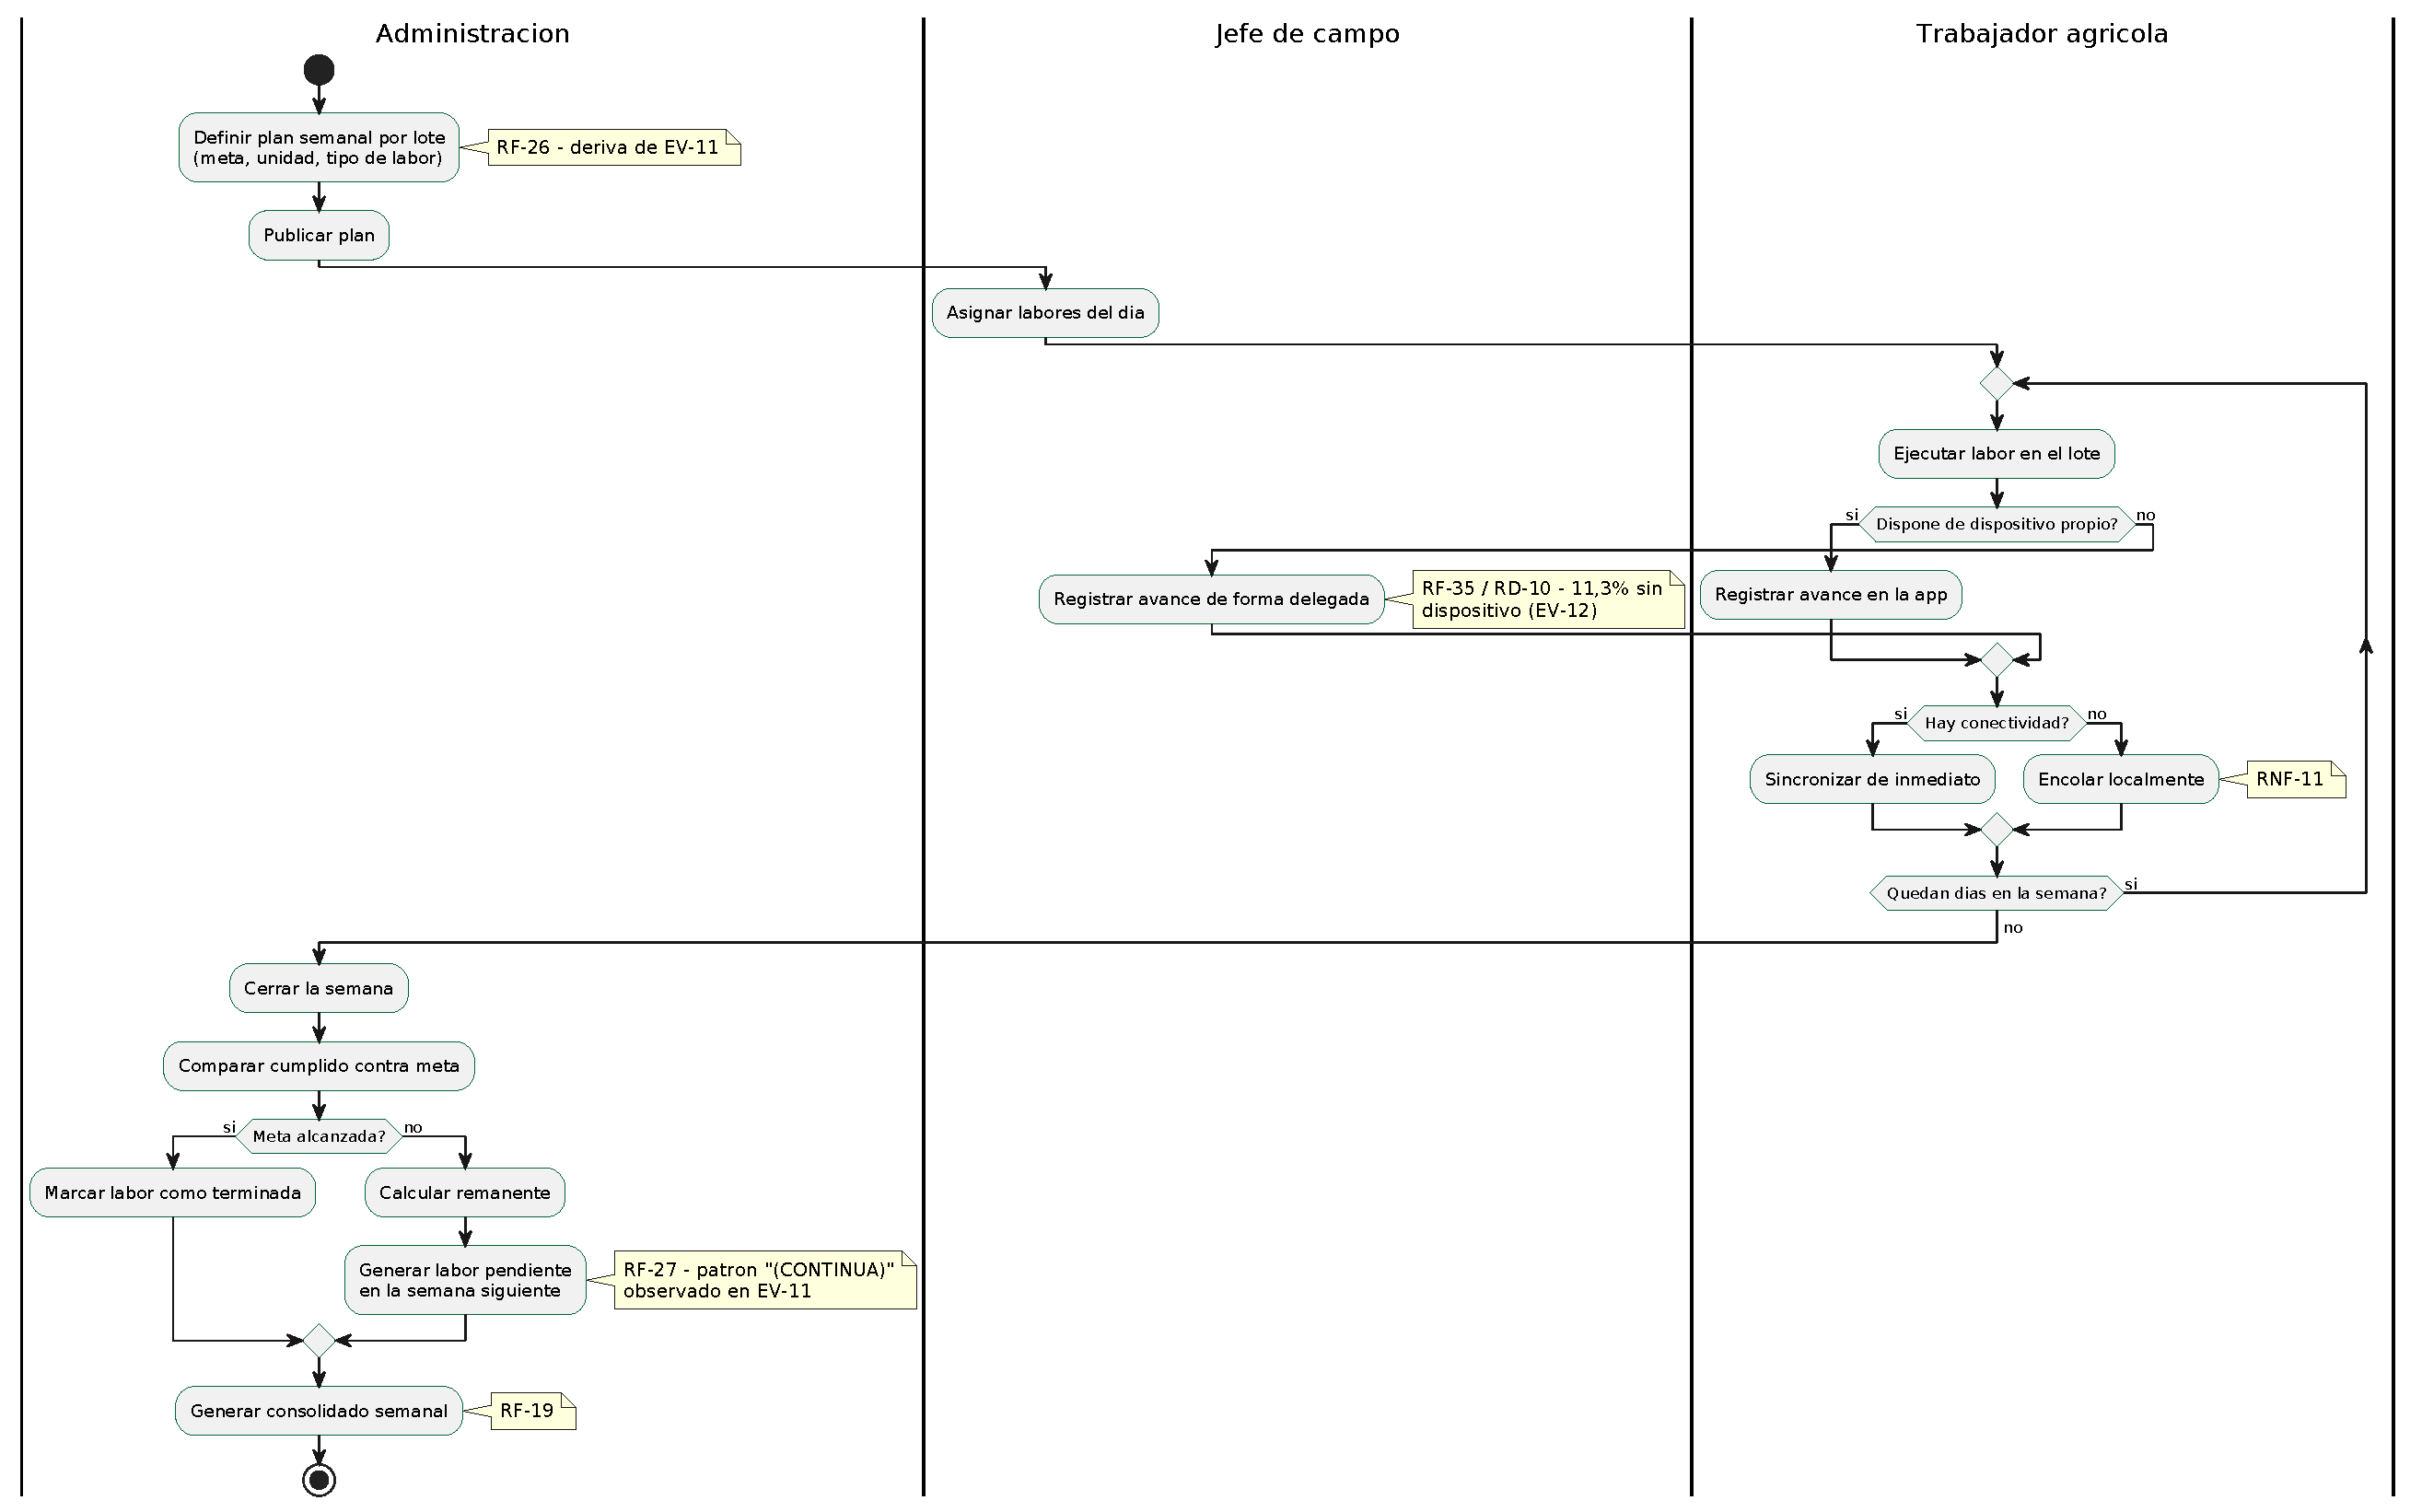
\includegraphics[width=1.0\textwidth]{img/actividad_ciclo_semanal}
\caption{Diagrama de actividad del ciclo semanal de planificación y ejecución de labores.}
\label{fig:actividad}
\end{figure}

% ---------------------------------------------------------------------
\subsection{Diagramas de estados}

Se modelan las dos entidades del dominio con ciclo de vida no trivial: el \textbf{racimo}, cuya
trayectoria determina el valor económico de la producción, y la \textbf{alerta}, cuyo ciclo refleja
la latencia real de verificación documentada en \id{EV-07}.

\begin{figure}[!htbp]
\centering
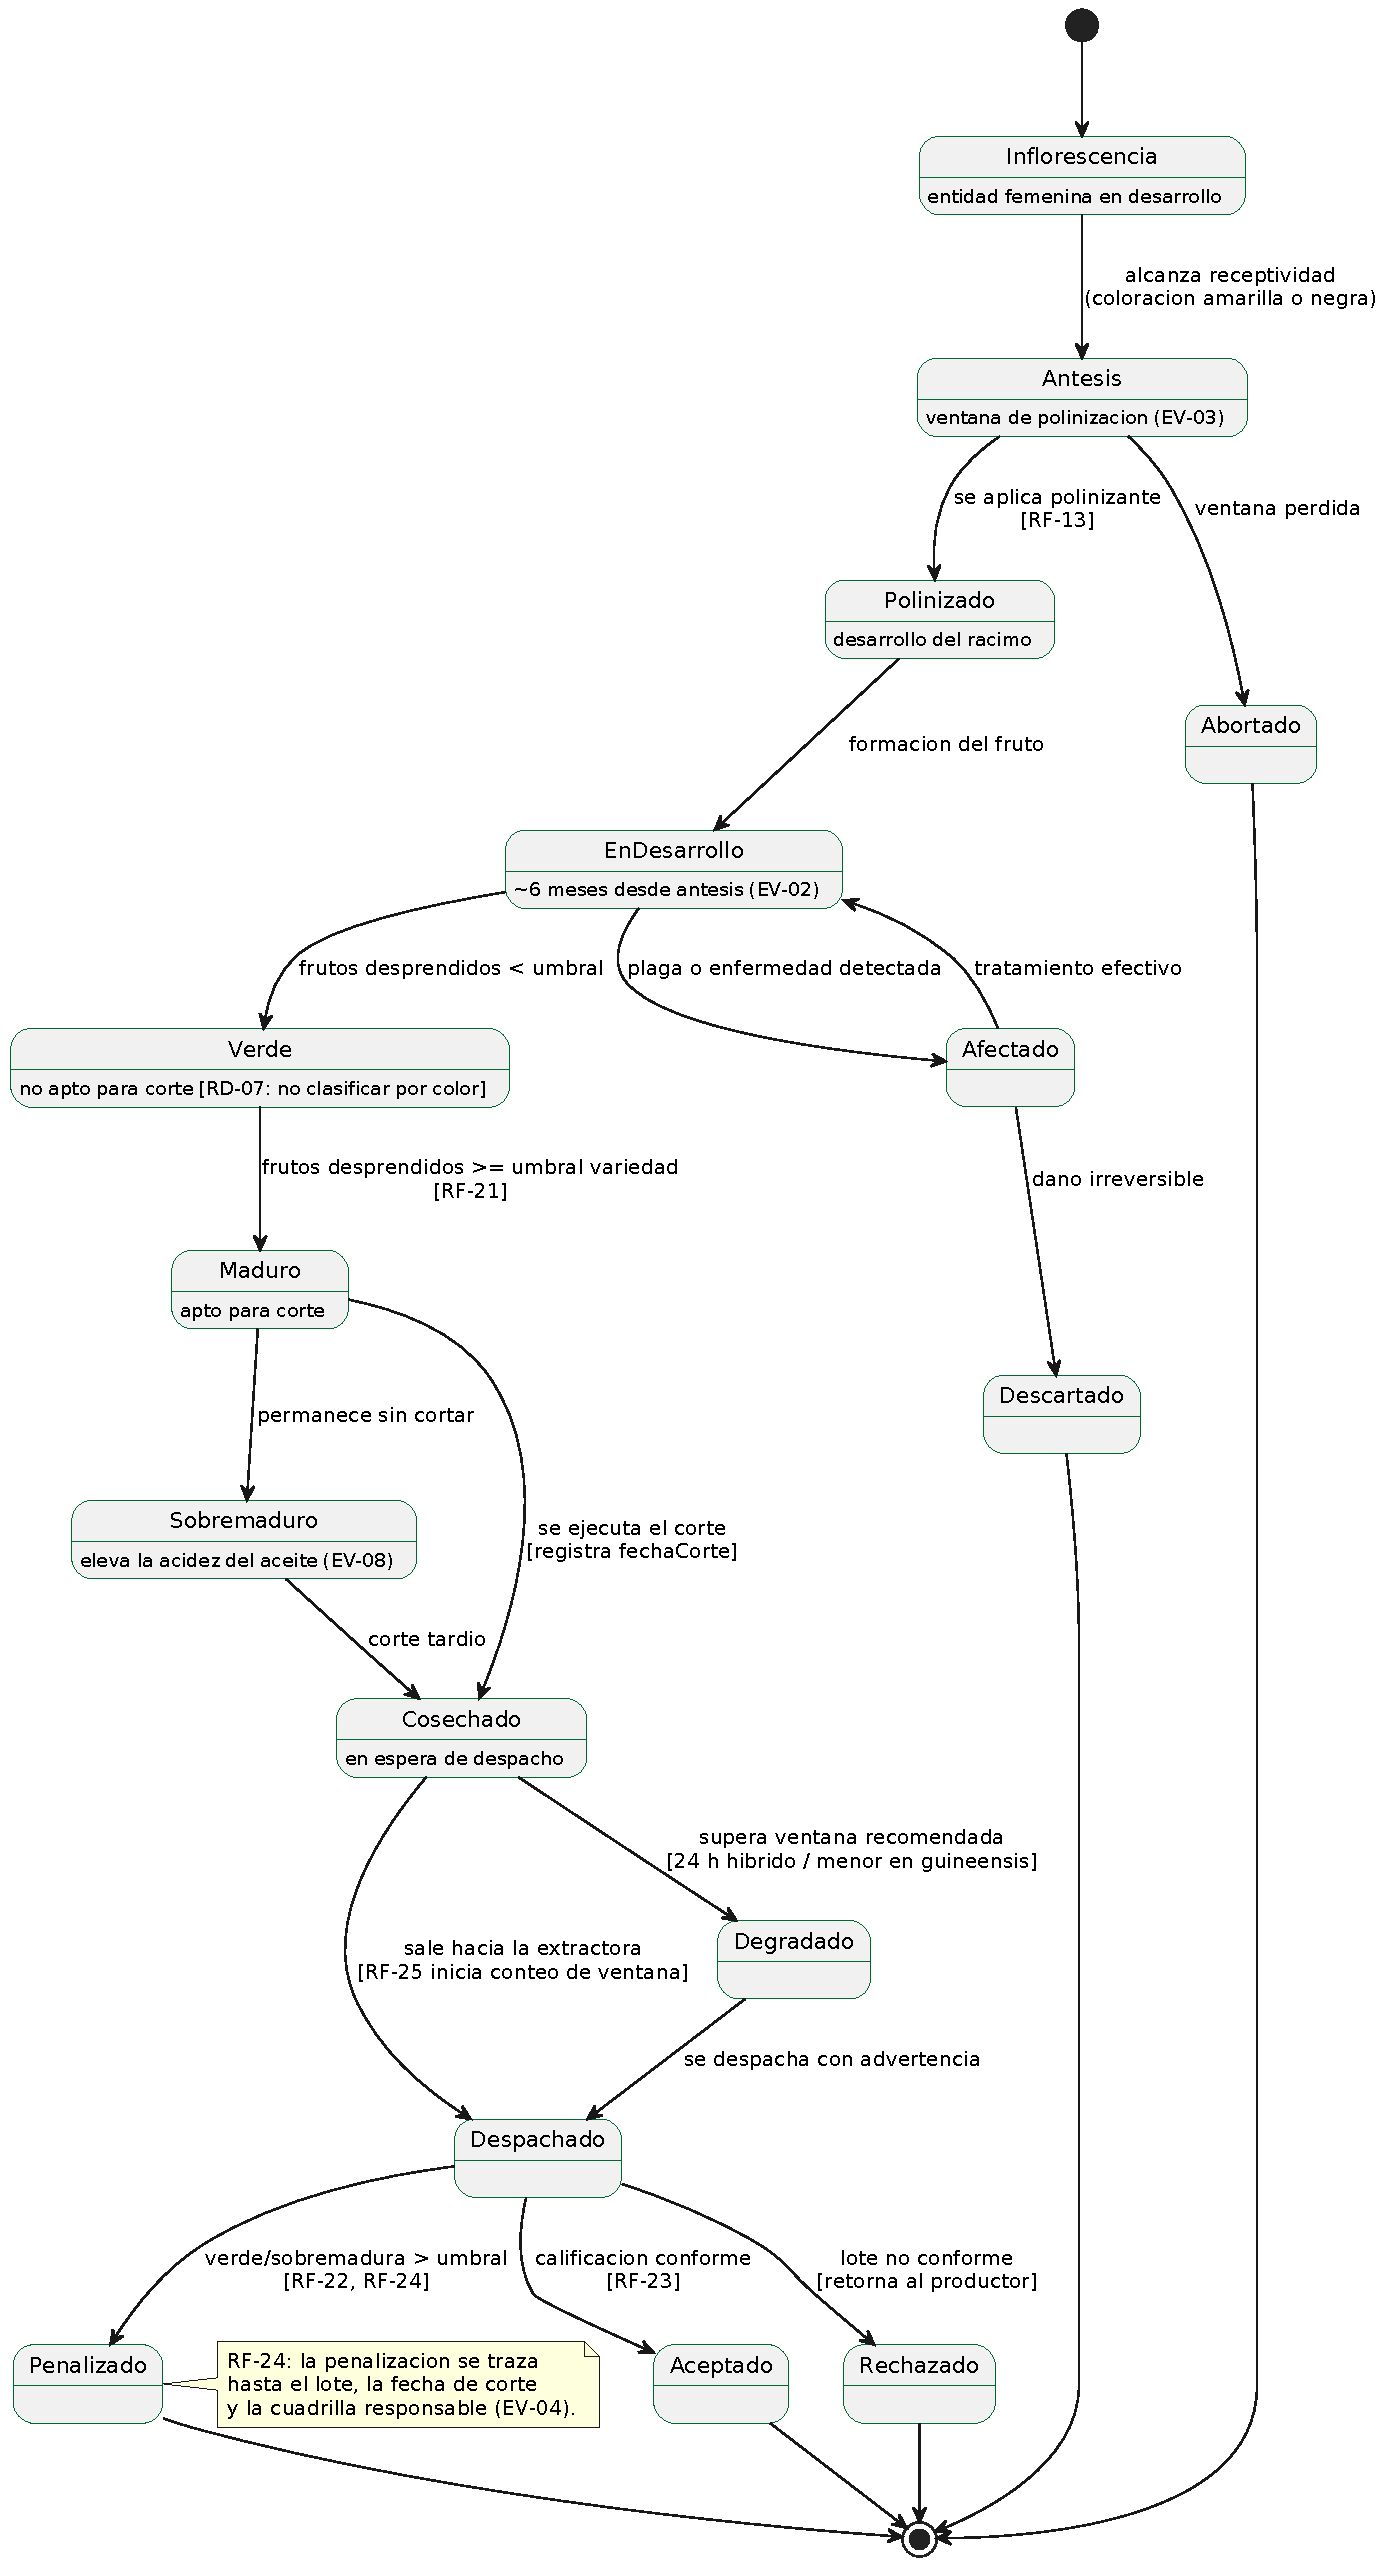
\includegraphics[width=0.67\textwidth]{img/estados_racimo}
\caption{Diagrama de estados del racimo, desde la inflorescencia hasta la calificación en la planta extractora.}
\label{fig:est_racimo}
\end{figure}

\begin{figure}[!htbp]
\centering
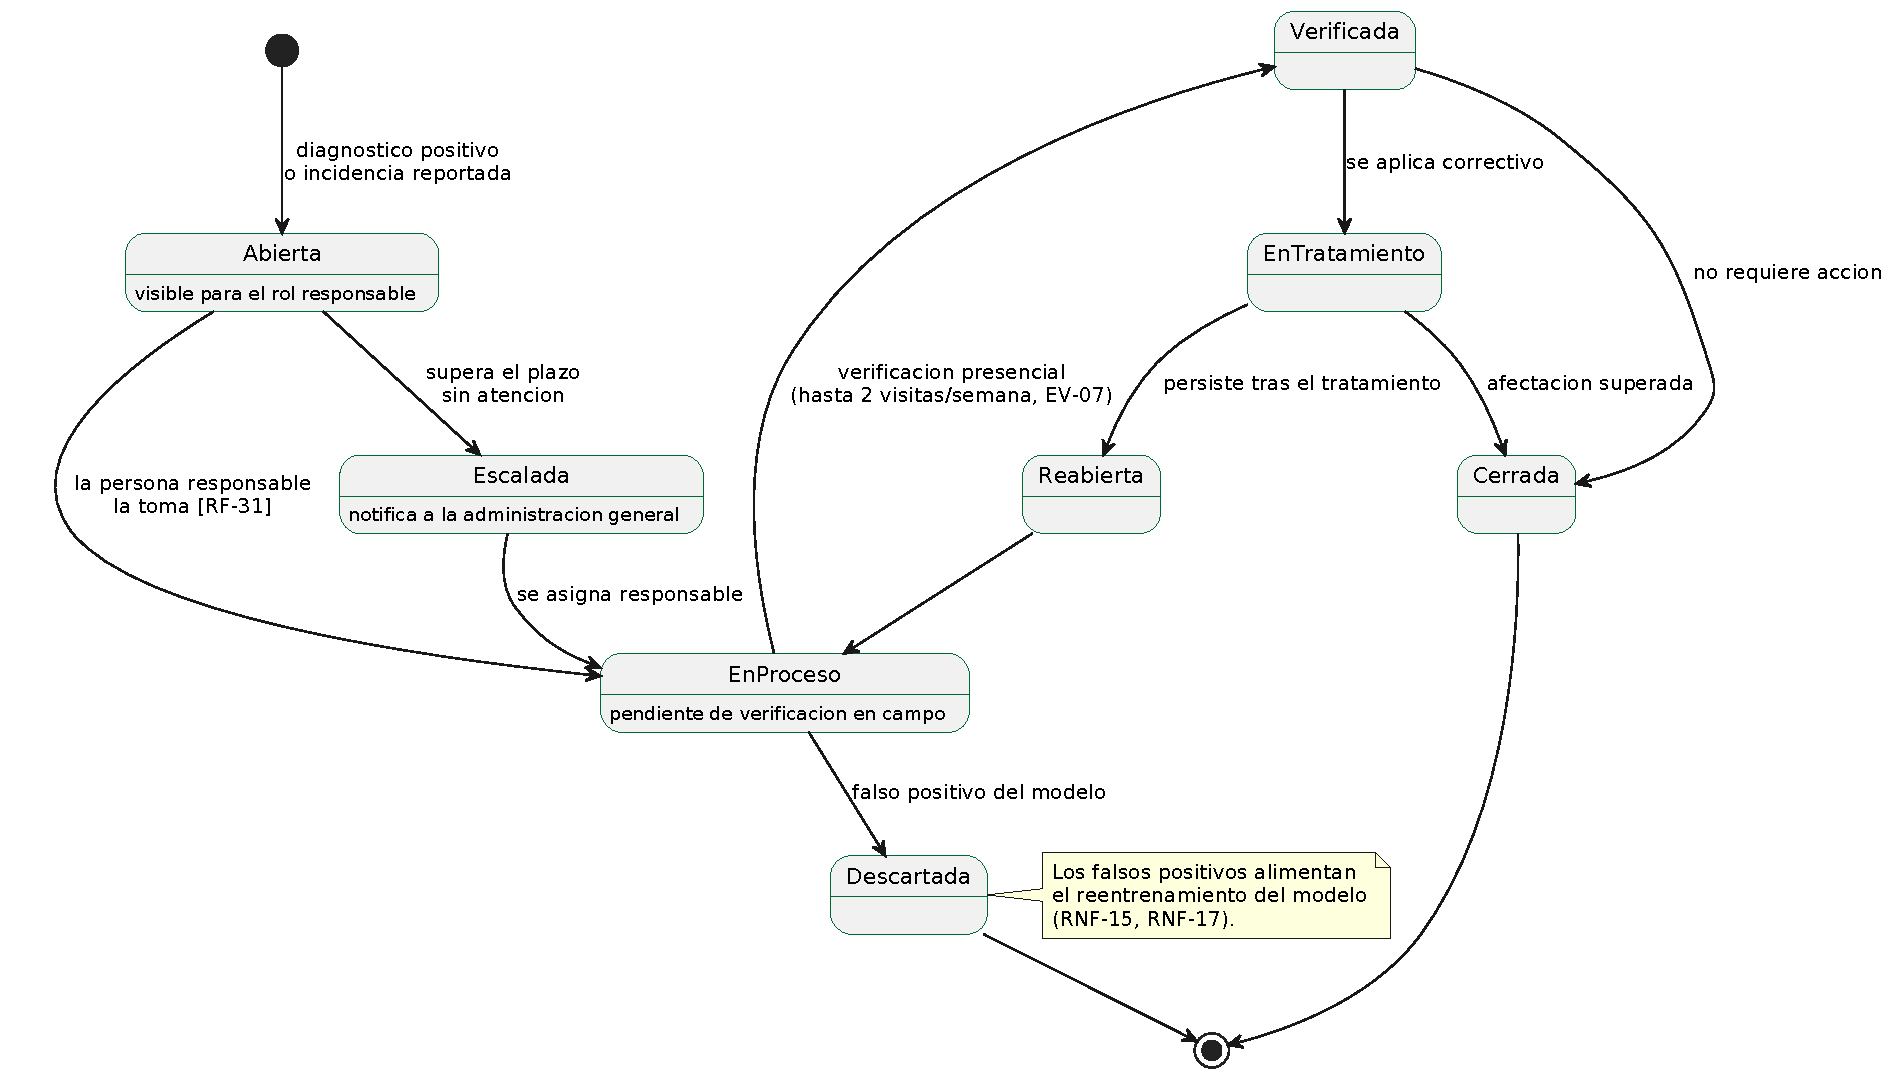
\includegraphics[width=1.0\textwidth]{img/estados_alerta}
\caption{Diagrama de estados de la alerta, con escalamiento por vencimiento de plazo y reapertura tras tratamiento inefectivo.}
\label{fig:est_alerta}
\end{figure}

\noindent
El estado \emph{Degradado} del racimo materializa el hallazgo de \id{EV-04} sobre la ventana entre
corte y entrega: el material híbrido tolera un intervalo mayor por su contenido de antioxidantes,
mientras que el \emph{guineensis} se deshidrata en dos o tres días. El estado \emph{Descartada} de
la alerta corresponde a los falsos positivos del modelo y alimenta el ciclo de reentrenamiento
previsto en \id{RNF-15} y \id{RNF-17}.

% ---------------------------------------------------------------------
\subsection{Diagrama de componentes}

\begin{figure}[!htbp]
\centering
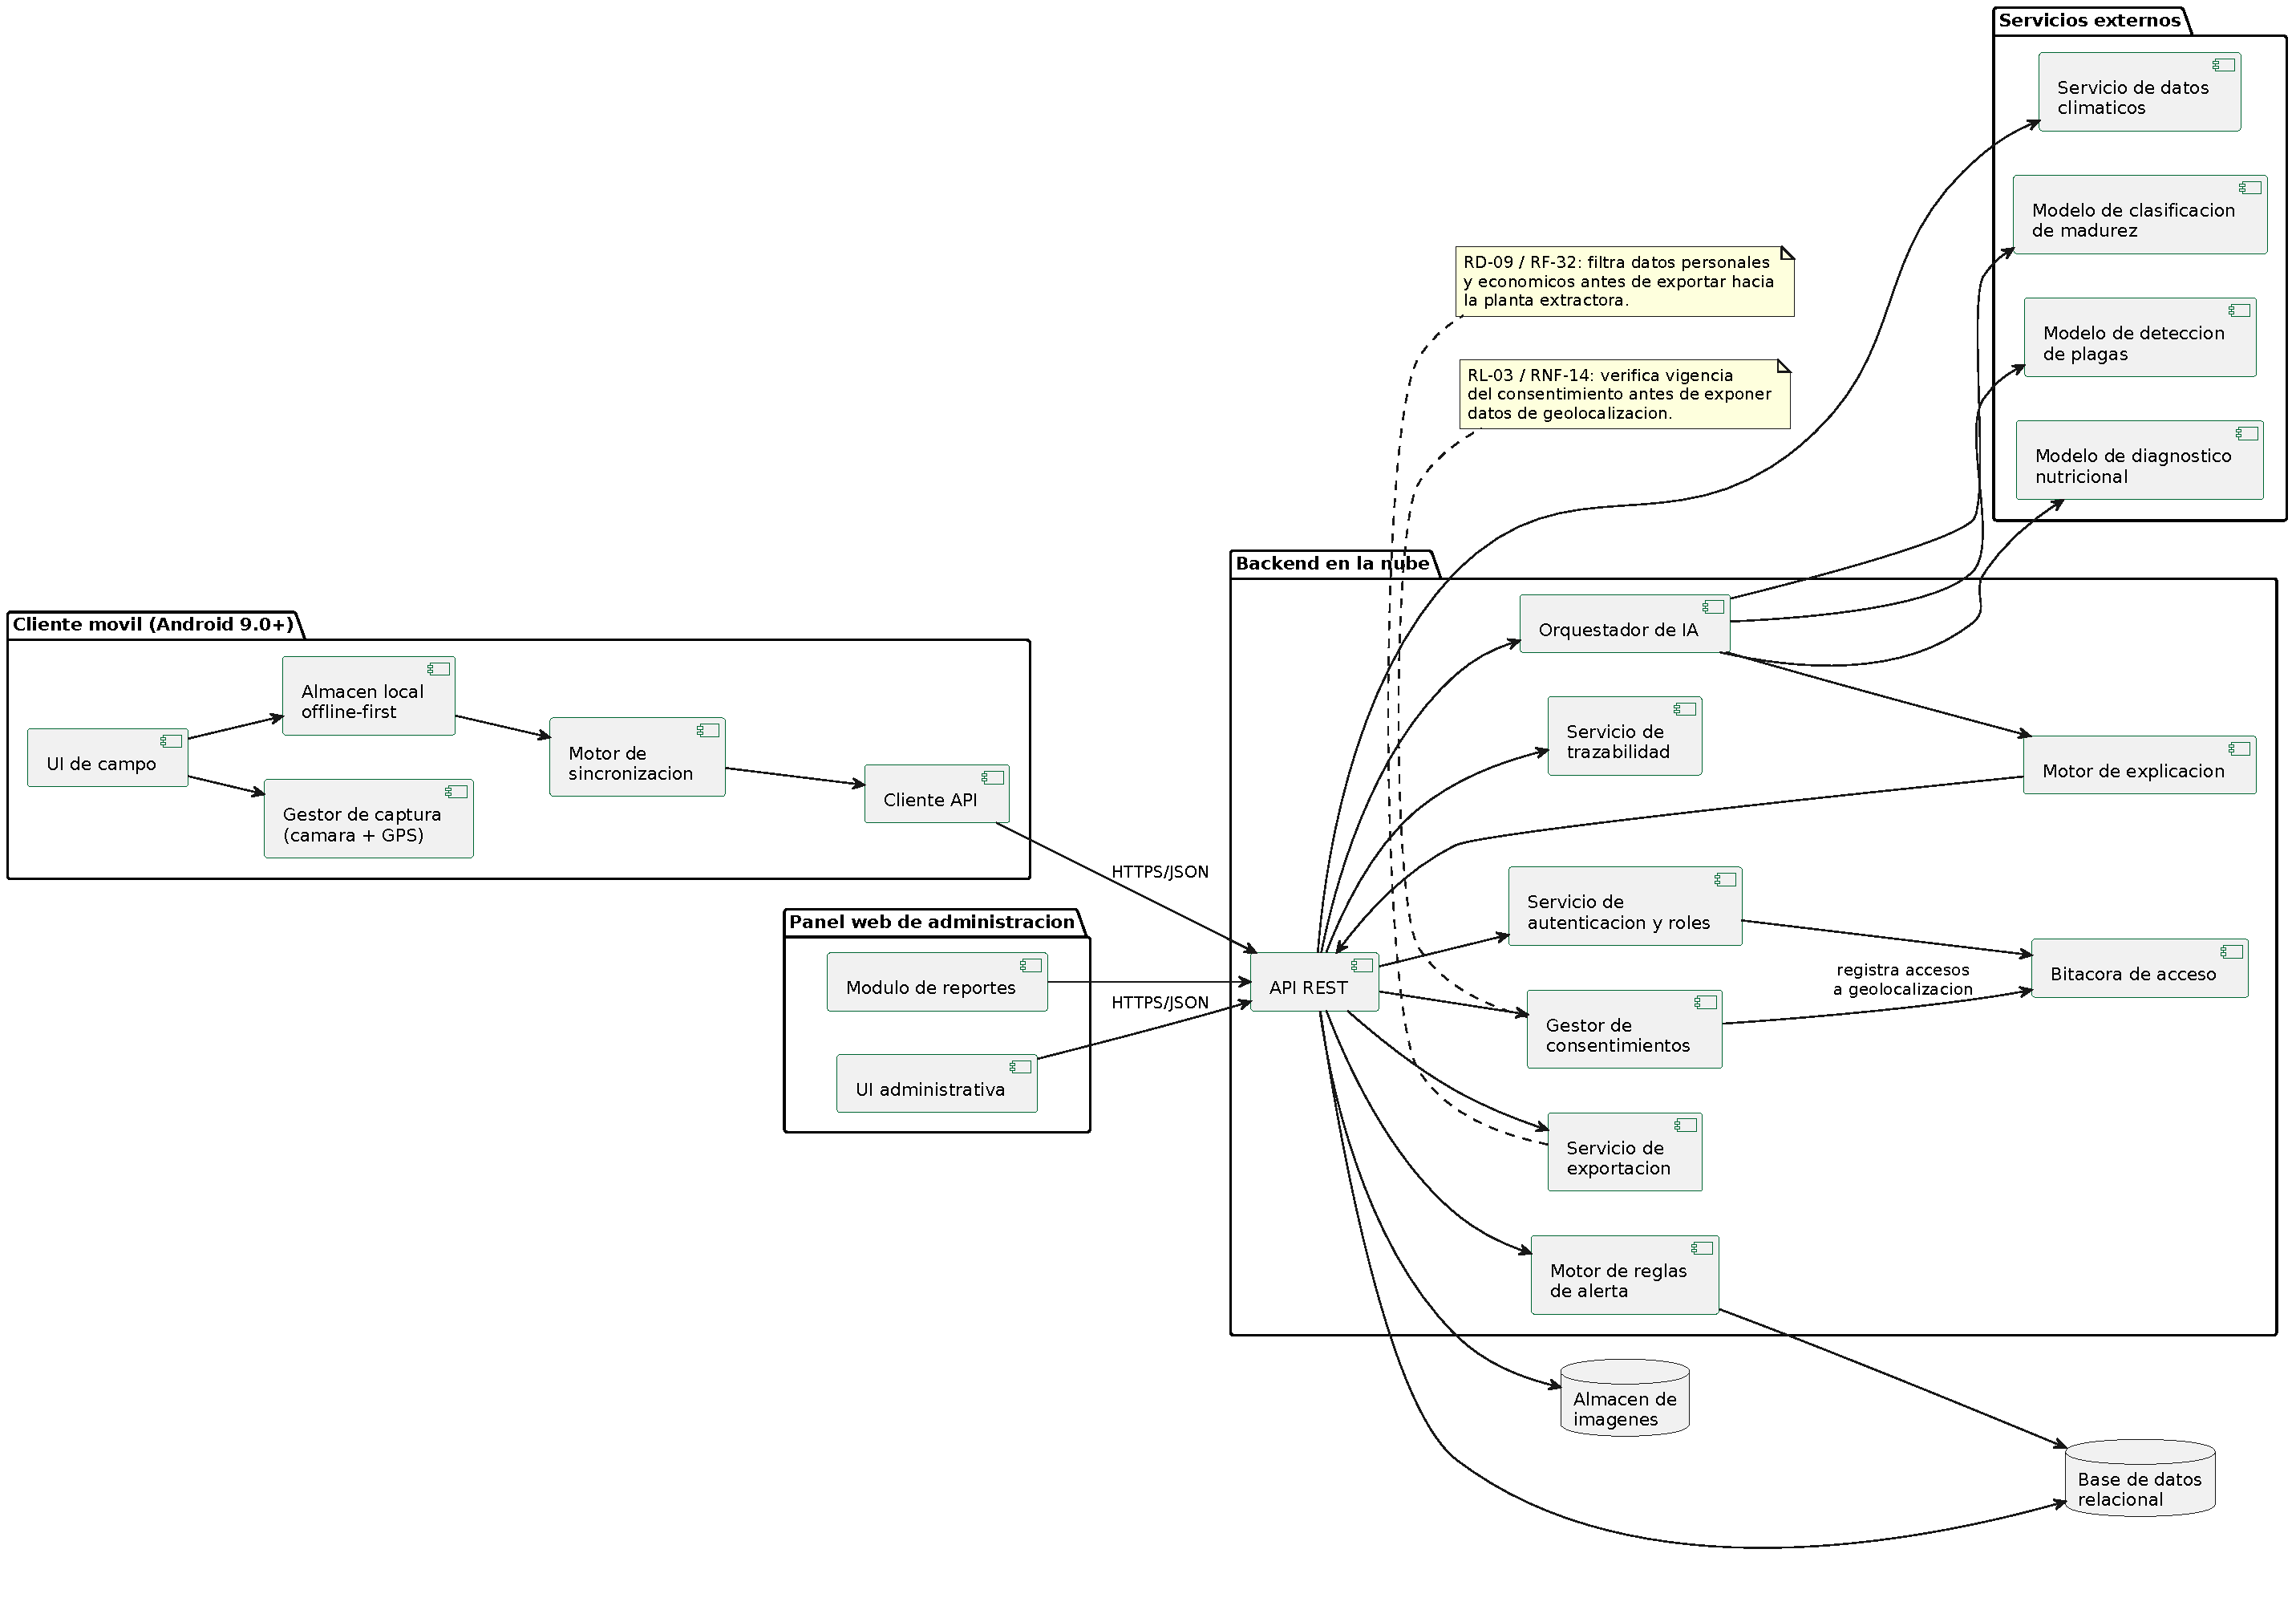
\includegraphics[width=1.0\textwidth]{img/componentes}
\caption{Diagrama de componentes del SIMPA.}
\label{fig:componentes}
\end{figure}

\noindent
Dos componentes merecen mención explícita por su origen normativo. El \emph{gestor de
consentimientos} verifica la vigencia antes de exponer cualquier dato de geolocalización y registra
todo acceso en la bitácora (\id{RL-03}, \id{RNF-14}). El \emph{servicio de exportación} filtra los
datos personales y económicos antes de generar el archivo destinado a la planta extractora
(\id{RD-09}, \id{RF-32}); su existencia como componente separado responde al criterio expreso de la
contraparte de que hay información que no puede compartirse (\id{EV-04}).

% ---------------------------------------------------------------------
\subsection{Diagrama de despliegue}

\begin{figure}[!htbp]
\centering
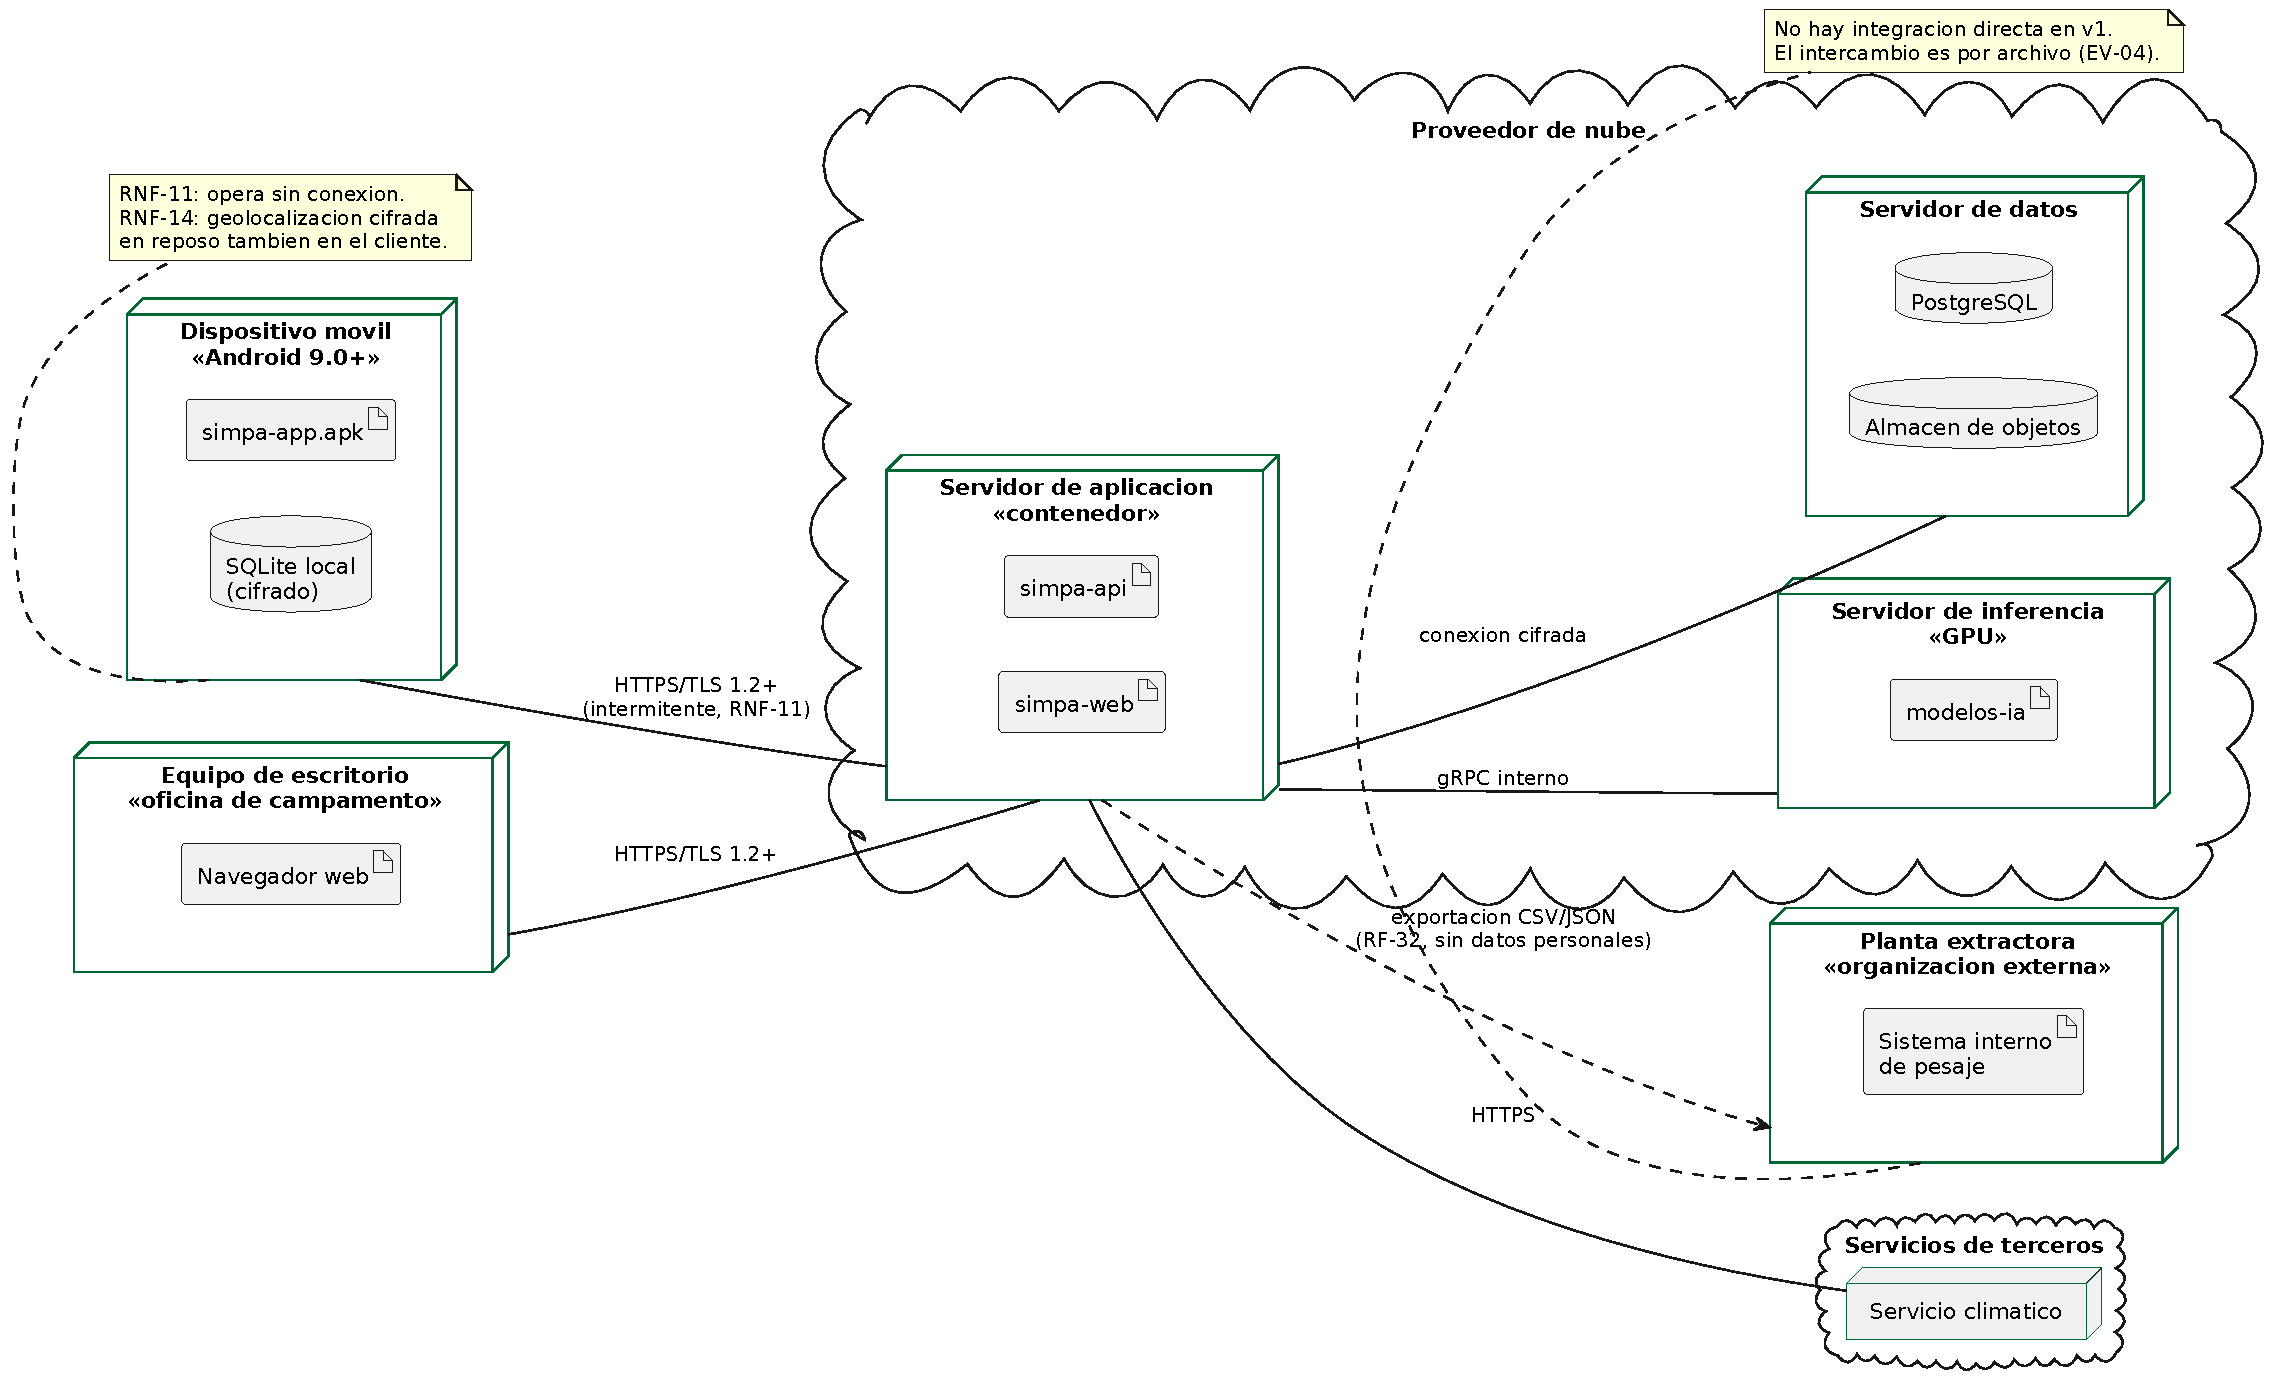
\includegraphics[width=1.0\textwidth]{img/despliegue}
\caption{Diagrama de despliegue del SIMPA.}
\label{fig:despliegue}
\end{figure}

\noindent
El enlace entre el dispositivo móvil y el servidor de aplicación se declara explícitamente como
\emph{intermitente}: el 74{,}2\% de las personas destinatarias no dispone de conectividad permanente
(\id{EV-12}). La planta extractora se representa como nodo externo sin integración directa; el
intercambio en la versión v1 se realiza por archivo, conforme a \id{RF-32}.

% ---------------------------------------------------------------------
\subsection{Cobertura del modelado}

\begin{longtable}{|L{4.6cm}|C{2.2cm}|C{2.2cm}|L{5.0cm}|}
\hline
\rowcolor{grisclaro}\textbf{Artefacto} & \textbf{Exigido} & \textbf{Entregado} & \textbf{Observación} \\
\hline
\endhead
Diagrama de casos de uso general & 1 & 1 & 8 actores, 18 casos de uso \\ \hline
Casos de uso detallados & 10 & 10 & Todos los \emph{Must}; $\geq 2$ flujos alternativos y $\geq 1$ excepción cada uno \\ \hline
Diagrama de clases refinado & 1 & 1 & 25 clases con atributos y operaciones \\ \hline
Diagramas de secuencia & CU \emph{Must} & 3 & CU-01, CU-03, CU-06 \\ \hline
Diagramas de actividad & Flujos principales & 1 & Ciclo semanal completo \\ \hline
Diagramas de estados & Entidades no triviales & 2 & Racimo y Alerta \\ \hline
Diagrama de componentes & 1 & 1 & --- \\ \hline
Diagrama de despliegue & 1 & 1 & --- \\ \hline
\caption{Cobertura del modelado UML frente a lo exigido en la §3.4 de la guía}
\end{longtable}


% =====================================================================
%  5. PRIORIZACION Y TRAZABILIDAD EXTENDIDA
% =====================================================================
% =====================================================================
%  SECCION 5 -- PRIORIZACION Y TRAZABILIDAD EXTENDIDA
%  Se incluye desde ERS_SRS_2A_v1.0.tex mediante % =====================================================================
%  SECCION 5 -- PRIORIZACION Y TRAZABILIDAD EXTENDIDA
%  Se incluye desde ERS_SRS_2A_v1.0.tex mediante % =====================================================================
%  SECCION 5 -- PRIORIZACION Y TRAZABILIDAD EXTENDIDA
%  Se incluye desde ERS_SRS_2A_v1.0.tex mediante \input{seccion5_priorizacion}
% =====================================================================

\newpage
\section{Priorización y trazabilidad extendida}

\subsection{Clasificación de requisitos}

El documento especifica 75 elementos de requisito, distribuidos como sigue.

\begin{longtable}{|L{4.2cm}|C{2.0cm}|L{8.4cm}|}
\hline
\rowcolor{grisclaro}\textbf{Tipo} & \textbf{Cantidad} & \textbf{Identificadores} \\
\hline
\endhead
Requisito funcional (RF) & 39 & \id{RF-01} a \id{RF-39} \\ \hline
Requisito no funcional (RNF) & 18 & \id{RNF-01} a \id{RNF-18} \\ \hline
Restricción de diseño (RD) & 10 & \id{RD-01} a \id{RD-10} \\ \hline
Requisito legal (RL) & 8 & \id{RL-01} a \id{RL-08} \\ \hline
\rowcolor{grisclaro}\textbf{Total} & \textbf{75} & \\ \hline
\caption{Clasificación de los requisitos por tipo}
\end{longtable}

\noindent
La distribución MoSCoW de los requisitos funcionales es de 21 \emph{Must}, 16 \emph{Should} y 2
\emph{Could}. Los cuatro requisitos incorporados a partir de la hoja de liquidación semanal
(\id{RF-36} a \id{RF-39}) se clasifican como \emph{Must} los dos primeros ---el catálogo de tarifas
es prerrequisito del cálculo de remuneración y la liquidación es el cierre del ciclo semanal--- y
como \emph{Should} los dos restantes. No hay requisitos funcionales clasificados como \emph{Won't}: las exclusiones de
alcance se enuncian a nivel de producto en la §1.2.4 y se argumentan en la §5.3.4.

% ---------------------------------------------------------------------
\subsection{Historias de usuario de los requisitos \emph{Must}}

Conforme a la §3.3 de la guía de la Entrega 3, cada requisito funcional de prioridad \emph{Must}
cuenta con una historia de usuario en formato Connextra, con los criterios INVEST verificados y un
escenario de aceptación redactado en Gherkin. Se especifican 19 historias (\id{HU-01} a
\id{HU-19}), con sus criterios de aceptación (\id{CA-01} a \id{CA-19}).

\begin{longtable}{|C{1.3cm}|C{1.3cm}|L{12.4cm}|}
\hline
\rowcolor{grisclaro}\textbf{HU} & \textbf{RF} & \textbf{Historia de usuario (Connextra) y escenario de aceptación (Gherkin)} \\
\hline
\endhead

\id{HU-01} & \id{RF-01} & \textbf{Como} persona trabajadora del cultivo, \textbf{quiero} acceder al sistema con mis credenciales, \textbf{para} usar únicamente las funciones que corresponden a mi labor. \newline \emph{\id{CA-01}:} \textbf{Dado} que existe una cuenta con rol ``trabajador agrícola'', \textbf{cuando} inicia sesión, \textbf{entonces} el menú no presenta ninguna opción de administración \textbf{y} un intento de acceso directo a esa ruta es rechazado. \\ \hline

\id{HU-02} & \id{RF-02} & \textbf{Como} administrador general, \textbf{quiero} registrar los lotes con su variedad y superficie, \textbf{para} poder asociarles labores, diagnósticos y cosechas. \newline \emph{\id{CA-02}:} \textbf{Dado} un lote recién registrado con variedad asignada, \textbf{cuando} se abre el formulario de registro de labor, \textbf{entonces} el lote aparece como opción seleccionable. \\ \hline

\id{HU-03} & \id{RF-03} & \textbf{Como} administrador general, \textbf{quiero} organizar al personal por equipos funcionales, \textbf{para} asignar labores y evaluar el desempeño por cuadrilla. \newline \emph{\id{CA-03}:} \textbf{Dado} un trabajador asignado al equipo de polinización, \textbf{cuando} se consulta el equipo, \textbf{entonces} la persona figura en él \textbf{y} es asignable a labores de ese tipo. \\ \hline

\id{HU-04} & \id{RF-04} & \textbf{Como} trabajador agrícola, \textbf{quiero} registrar la labor que ejecuté en el lote, \textbf{para} que quede constancia sin depender de una libreta de papel. \newline \emph{\id{CA-04}:} \textbf{Dado} que ejecuté chapia en el lote 3, \textbf{cuando} registro la labor con su cantidad, \textbf{entonces} queda vinculada al lote, la fecha y mi identificación \textbf{y} aparece en el historial del lote. \\ \hline

\id{HU-05} & \id{RF-05} & \textbf{Como} técnico fitosanitario, \textbf{quiero} registrar el monitoreo sanitario del lote, \textbf{para} dejar trazabilidad de las revisiones y de las incidencias detectadas. \newline \emph{\id{CA-05}:} \textbf{Dado} un monitoreo con incidencia marcada, \textbf{cuando} se filtran los lotes con incidencia abierta, \textbf{entonces} ese lote aparece en el resultado. \\ \hline

\id{HU-06} & \id{RF-07} & \textbf{Como} asistente de administración, \textbf{quiero} fotografiar una palma afectada y obtener el diagnóstico, \textbf{para} identificar la plaga sin depender de conocimiento especializado. \newline \emph{\id{CA-06}:} \textbf{Dado} que capturo la imagen de una palma con afectación conocida, \textbf{cuando} solicito el análisis, \textbf{entonces} el sistema devuelve la clase, el nivel de confianza y una explicación de no más de 60 palabras \textbf{y} registra el diagnóstico con lote y fecha. \\ \hline

\id{HU-07} & \id{RF-08} & \textbf{Como} asesor técnico, \textbf{quiero} fotografiar una hoja y conocer la deficiencia nutricional, \textbf{para} decidir qué aplicar sin esperar el análisis de laboratorio. \newline \emph{\id{CA-07}:} \textbf{Dado} el lote con variedad asignada, \textbf{cuando} envío la imagen de una hoja con deficiencia conocida, \textbf{entonces} el sistema indica el elemento deficiente, propone una corrección \textbf{y} explica qué signo foliar la sustenta. \\ \hline

\id{HU-08} & \id{RF-10} & \textbf{Como} asesor técnico, \textbf{quiero} que el sistema conozca la variedad de cada lote, \textbf{para} que los umbrales de diagnóstico correspondan al material sembrado. \newline \emph{\id{CA-08}:} \textbf{Dado} un lote de variedad \emph{guineensis}, \textbf{cuando} se clasifica un racimo, \textbf{entonces} el umbral aplicado es de 3 frutos desprendidos; \textbf{y dado} un lote híbrido, \textbf{entonces} el umbral aplicado es de 5. \\ \hline

\id{HU-09} & \id{RF-12} & \textbf{Como} administrador general, \textbf{quiero} recibir alertas ante una afectación detectada, \textbf{para} intervenir antes de que se propague. \newline \emph{\id{CA-09}:} \textbf{Dado} un diagnóstico positivo registrado, \textbf{cuando} se completa el análisis, \textbf{entonces} se crea una alerta con lote, tipo, criticidad y estado abierto \textbf{y} resulta visible para el rol responsable. \\ \hline

\id{HU-10} & \id{RF-13} & \textbf{Como} jefe de polinización, \textbf{quiero} registrar el estado de la antesis y la verificación visual, \textbf{para} controlar la calidad de la labor que determina la producción. \newline \emph{\id{CA-10}:} \textbf{Dado} un lote en etapa de polinización, \textbf{cuando} se registra la jornada con estado de antesis, \textbf{entonces} el registro queda asociado al lote, la fecha y la persona \textbf{y} es consultable por fecha. \\ \hline

\id{HU-11} & \id{RF-14} & \textbf{Como} polinizador, \textbf{quiero} que el conteo de flores se calcule solo, \textbf{para} no perder rendimiento anotando planta por planta. \newline \emph{\id{CA-11}:} \textbf{Dado} que trabajé la jornada con rastreo activo, \textbf{cuando} cierro la jornada, \textbf{entonces} el sistema calcula el total de flores a partir de las marcaciones \textbf{y} no me solicita ningún registro manual por planta. \\ \hline

\id{HU-12} & \id{RF-18} & \textbf{Como} administrador general, \textbf{quiero} estimar la producción del período, \textbf{para} planificar la cosecha y la mano de obra necesaria. \newline \emph{\id{CA-12}:} \textbf{Dado} un censo de flores registrado y la variedad del lote, \textbf{cuando} solicito la estimación, \textbf{entonces} el sistema devuelve el tonelaje estimado del período \textbf{y} el supuesto de rendimiento empleado. \\ \hline

\id{HU-13} & \id{RF-19} & \textbf{Como} administrador general, \textbf{quiero} generar el consolidado semanal, \textbf{para} tomar decisiones sin recopilar reportes dispersos de mensajería. \newline \emph{\id{CA-13}:} \textbf{Dado} que existen registros en la semana, \textbf{cuando} genero el reporte, \textbf{entonces} obtengo labores, avance, producción y alertas del período \textbf{y} puedo exportarlo a PDF o a hoja de cálculo. \\ \hline

\id{HU-14} & \id{RF-21} & \textbf{Como} cosechador, \textbf{quiero} saber si un racimo está en punto de corte, \textbf{para} no cortar fruta verde que será penalizada. \newline \emph{\id{CA-14}:} \textbf{Dado} un lote híbrido, \textbf{cuando} fotografío la parte basal de un racimo con 4 frutos desprendidos, \textbf{entonces} el sistema lo clasifica como verde \textbf{y} explica que el umbral de la variedad es de 5. \\ \hline

\id{HU-15} & \id{RF-22} & \textbf{Como} administrador general, \textbf{quiero} conocer el porcentaje estimado de fruta verde antes de despachar, \textbf{para} evitar la penalización del lote en la planta extractora. \newline \emph{\id{CA-15}:} \textbf{Dado} un umbral de penalización del 3\%, \textbf{cuando} el porcentaje estimado del lote alcanza ese valor, \textbf{entonces} el sistema emite alerta preventiva \textbf{y} desaconseja el despacho. \\ \hline

\id{HU-16} & \id{RF-26} & \textbf{Como} administrador general, \textbf{quiero} registrar el presupuesto semanal de labores, \textbf{para} contrastar lo planificado con lo efectivamente ejecutado. \newline \emph{\id{CA-16}:} \textbf{Dado} un plan con meta de 1.123 coronas en el lote 3, \textbf{cuando} cierro la semana con 800 cumplidas, \textbf{entonces} el sistema reporta un cumplimiento del 71,2\% \textbf{y} un remanente de 323 coronas. \\ \hline

\id{HU-17} & \id{RF-28} & \textbf{Como} trabajador agrícola, \textbf{quiero} registrar mi avance en la unidad propia de cada labor, \textbf{para} que mi trabajo se contabilice como corresponde. \newline \emph{\id{CA-17}:} \textbf{Dado} que ejecuté 120 coronas, \textbf{cuando} registro el avance, \textbf{entonces} la cantidad se acumula a mi total semanal en la unidad ``coronas'' \textbf{y} el sistema rechaza una unidad incompatible con el tipo de labor. \\ \hline

\id{HU-18} & \id{RF-30} & \textbf{Como} asistente de administración, \textbf{quiero} reportar una afectación con foto y ubicación, \textbf{para} poder volver al punto exacto en mi siguiente visita. \newline \emph{\id{CA-18}:} \textbf{Dado} que reporto una incidencia con GPS activo, \textbf{cuando} la consulto días después, \textbf{entonces} recupero su fotografía y sus coordenadas \textbf{y} la incidencia figura en mi lista de pendientes de verificación. \\ \hline

\id{HU-19} & \id{RF-35} & \textbf{Como} jefe de campo, \textbf{quiero} registrar el avance de quien no tiene teléfono, \textbf{para} que ninguna persona quede sin registrar su trabajo. \newline \emph{\id{CA-19}:} \textbf{Dado} un trabajador sin dispositivo propio, \textbf{cuando} registro su avance de forma delegada, \textbf{entonces} el avance se atribuye a esa persona en su consolidado \textbf{y} la bitácora conserva mi identificación como registrador. \\ \hline
\caption{Historias de usuario y criterios de aceptación de los requisitos \emph{Must}}
\end{longtable}

\subsubsection{Verificación de los criterios INVEST}

Las diecinueve historias fueron evaluadas contra los seis criterios INVEST. La tabla siguiente
reporta el resultado y documenta las tres historias que requirieron ajuste.

\begin{longtable}{|L{2.4cm}|C{1.6cm}|L{11.0cm}|}
\hline
\rowcolor{grisclaro}\textbf{Criterio} & \textbf{Cumple} & \textbf{Observación} \\
\hline
\endhead
Independiente & 16 / 19 & \id{HU-11} depende de \id{HU-10}, \id{HU-15} de \id{HU-14} y \id{HU-17} de \id{HU-04}. Se documenta la dependencia en la matriz en lugar de forzar la independencia, dado que responde a la secuencia real del proceso. \\ \hline
Negociable & 19 / 19 & Ninguna historia prescribe solución técnica; los umbrales son parametrizables (\id{RD-08}). \\ \hline
Valiosa & 19 / 19 & Cada historia declara el beneficio esperado y se traza a evidencia de campo. \\ \hline
Estimable & 19 / 19 & Todas admiten estimación en la escala Fibonacci empleada en el cálculo WSJF de la §5.3.3. \\ \hline
Pequeña & 17 / 19 & \id{HU-06} y \id{HU-07} superan el tamaño recomendado por incluir el componente de IA; se sugiere descomponerlas en captura, inferencia y explicación durante la planificación de la implementación. \\ \hline
Verificable & 19 / 19 & Todas cuentan con escenario Gherkin con criterio observable. \\ \hline
\caption{Verificación de los criterios INVEST sobre las historias de usuario}
\end{longtable}

% ---------------------------------------------------------------------
\subsection{Priorización combinada}

La priorización emplea tres instrumentos complementarios: MoSCoW para el compromiso de alcance, el
modelo de Kano para la relación con la satisfacción del cliente, y WSJF para el orden de
implementación.

\subsubsection{Justificación de la clasificación MoSCoW}

\textbf{\emph{Must} (19 RF).} Corresponden a tres condiciones. Primero, la \textbf{base operativa
indispensable}: sin autenticación por rol (\id{RF-01}), estructura de lotes (\id{RF-02}), personal
(\id{RF-03}) y registro de labor y avance (\id{RF-04}, \id{RF-28}, \id{RF-35}) el sistema no
sustituye al proceso manual que pretende reemplazar. Segundo, el \textbf{diferencial de valor}: el
análisis por imagen (\id{RF-07}, \id{RF-08}, \id{RF-21}) y las alertas (\id{RF-12}) son las
funciones mejor valoradas por el personal en el cuestionario ($4{,}31$ y $4{,}27$ sobre 5,
\id{EV-12}) y las señaladas de forma independiente por la administración (\id{EV-01}) y la asesoría
técnica (\id{EV-02}). Tercero, la \textbf{consecuencia económica directa}: la polinización determina
la producción de la finca (\id{EV-03}), su conteo condiciona la evaluación del trabajo
(\id{RF-13}, \id{RF-14}), y el porcentaje de fruta verde determina la penalización del lote en la
planta extractora (\id{RF-22}, \id{EV-04}).

\textbf{\emph{Should} (14 RF).} Aportan valor sustantivo pero el sistema entrega su propuesta de
valor sin ellos en la primera versión: seguimiento de etapas, ficha de plaga, análisis de
suelo, recorridos, evaluación de desempeño, clima, historial, registro del ticket de la extractora,
trazabilidad de la penalización, ventana corte-entrega, arrastre semanal, consulta de remuneración,
lista de pendientes y exportación hacia la extractora.

\textbf{\emph{Could} (2 RF).} \id{RF-33} (guía de remisión) y \id{RF-34} (solicitud de insumos) son
mejoras deseables de bajo acoplamiento con el núcleo.

\textbf{\emph{Won't} en esta versión.} Se excluyen explícitamente y con argumento: la
\textbf{gestión de nómina y pago}, porque el sistema calcula el avance pero la liquidación
involucra información laboral y tributaria cuyo tratamiento excede el consentimiento obtenido
(\id{RD-04}, \id{RL-02}); la \textbf{facturación y contabilidad}, por no corresponder al manejo del
cultivo; la \textbf{comercialización de la producción}, que se negocia fuera del sistema; la
\textbf{integración directa con el sistema de la planta extractora}, porque pertenece a una
organización externa con sistema propio y su interfaz no está disponible (\id{EV-04}); y la
\textbf{operación multi-finca}, que el cliente administra pero que no forma parte del alcance
acordado para la v1 (§1.2.2).

\subsubsection{Modelo de Kano}

La clasificación se sustenta en la distancia entre la valoración declarada en el cuestionario y la
expectativa implícita del proceso actual.

\begin{longtable}{|L{2.8cm}|L{5.4cm}|L{7.0cm}|}
\hline
\rowcolor{grisclaro}\textbf{Categoría} & \textbf{Requisitos} & \textbf{Fundamento} \\
\hline
\endhead
Básica & \id{RF-01}, \id{RF-02}, \id{RF-03}, \id{RF-04} & Su ausencia genera rechazo, su presencia no genera entusiasmo. El registro de labor ya existe en papel: el sistema debe igualarlo, no impresiona por hacerlo. \\ \hline
De desempeño & \id{RF-19}, \id{RF-26}, \id{RF-28}, \id{RF-29}, \id{RF-13} & La satisfacción crece de forma proporcional a la calidad de ejecución. Valoración intermedia en el cuestionario ($3{,}95$ para el registro de labores). \\ \hline
\rowcolor{grisclaro}De deleite & \id{RF-07}, \id{RF-08}, \id{RF-12}, \id{RF-21} & Generan entusiasmo desproporcionado respecto de la expectativa. Son las funciones mejor valoradas ($4{,}27$ y $4{,}31$) y las únicas mencionadas de forma espontánea por los cinco perfiles entrevistados. \\ \hline
Indiferente & \id{RF-33}, \id{RF-34} & No inciden en la satisfacción percibida por la persona usuaria final. \\ \hline
De rechazo potencial & \id{RF-15} & El rastreo de recorridos puede generar insatisfacción: el 25{,}8\% del personal manifiesta reservas (\id{EV-12}). Se mitiga con consentimiento revocable (\id{RL-03}). \\ \hline
\caption{Clasificación de los requisitos según el modelo de Kano}
\end{longtable}

\noindent
La clasificación de \id{RF-15} como \emph{requisito de rechazo potencial} es deliberada y
constituye un hallazgo. La funcionalidad fue solicitada por la administración (\id{EV-01},
\id{EV-02}) y por la jefatura de polinización (\id{EV-03}), pero una de cada cuatro personas
destinatarias expresa reservas sobre ella. Kano permite representar esta tensión: un requisito puede
ser valioso para quien lo solicita y adverso para quien lo padece. La mitigación no es técnica sino
de diseño de la relación: consentimiento específico, revocable y sin consecuencia laboral.

\subsubsection{Valor de negocio mediante WSJF}

Se aplica el método del Trabajo Ponderado Más Corto Primero:
\[
\mathrm{WSJF} = \frac{\text{Valor de negocio} + \text{Criticidad temporal} + \text{Reducción de riesgo}}{\text{Tamaño del trabajo}}
\]
Los cuatro componentes se puntúan en escala Fibonacci (1, 2, 3, 5, 8, 13). La tabla presenta los
diez requisitos evaluados de mayor valor de negocio, ordenados de forma descendente por WSJF.

\begin{longtable}{|C{1.4cm}|C{1.3cm}|C{1.3cm}|C{1.3cm}|C{1.3cm}|C{1.4cm}|L{5.4cm}|}
\hline
\rowcolor{grisclaro}\textbf{RF} & \textbf{Valor} & \textbf{Crit. temp.} & \textbf{Red. riesgo} & \textbf{Tamaño} & \textbf{WSJF} & \textbf{Justificación} \\
\hline
\endhead
\id{RF-35} & 5 & 8 & 8 & 3 & \textbf{7,00} & Bajo costo y alto impacto: sin él, el 11,3\% del personal queda excluido del sistema (\id{EV-12}). \\ \hline
\id{RF-21} & 13 & 13 & 8 & 8 & \textbf{4,25} & Evita la penalización económica del lote; la temporada de baja producción (jul.--oct.) es cuando más fruta verde se corta (\id{EV-04}). \\ \hline
\id{RF-22} & 13 & 13 & 8 & 8 & \textbf{4,25} & Actúa antes del despacho, momento en que la pérdida aún es evitable. \\ \hline
\id{RF-04} & 8 & 8 & 5 & 5 & \textbf{4,20} & Base de todo el registro operativo; sin él no hay datos para ninguna otra función. \\ \hline
\id{RF-12} & 8 & 8 & 5 & 5 & \textbf{4,20} & Función mejor valorada del cuestionario (4,31/5). \\ \hline
\id{RF-01} & 5 & 8 & 8 & 5 & \textbf{4,20} & Precondición técnica y legal de todo lo demás (\id{RL-01}). \\ \hline
\id{RF-07} & 13 & 8 & 8 & 8 & \textbf{3,62} & Mayor dificultad declarada por el personal (40,3\%, \id{EV-12}). \\ \hline
\id{RF-28} & 8 & 5 & 5 & 5 & \textbf{3,60} & Habilita el cálculo de cumplimiento y de remuneración por avance. \\ \hline
\id{RF-14} & 13 & 8 & 5 & 8 & \textbf{3,25} & La polinización determina la producción; el conteo manual afecta el rendimiento (\id{EV-03}). \\ \hline
\id{RF-08} & 8 & 5 & 5 & 8 & \textbf{2,25} & Alto valor técnico, pero el diagnóstico nutricional admite mayor demora que el sanitario. \\ \hline

\caption{Valor de negocio mediante WSJF (diez requisitos de mayor prioridad)}
\end{longtable}

\noindent
\textbf{Lectura del resultado.} \id{RF-35} y \id{RF-10} encabezan el orden de implementación con un
WSJF de 7,00 cada uno,
pese a no ser el requisito de mayor valor de negocio. La razón es su tamaño reducido frente a un
impacto alto: se trata de una variante del formulario de registro que evita excluir a una de cada
nueve personas destinatarias. \id{RF-10} alcanza la misma posición por una razón distinta: es
prerrequisito de \id{RF-21}, dado que el umbral de desprendimiento se obtiene de la variedad del
lote. El método revela así una dependencia técnica que ni MoSCoW ni Kano hacen visible.

Ambos casos ilustran la utilidad del método frente a una priorización basada únicamente en valor
percibido, que los habría situado muy por debajo. La lectura inversa también es informativa:
\id{RF-07} y \id{RF-08}, las dos funciones mejor valoradas por las personas usuarias, obtienen WSJF
de 3,62 y 2,25 por su elevado tamaño de trabajo. Esto no altera su condición de \emph{Must}, pero
indica que el desarrollo debe iniciarse por la base operativa mientras los componentes de
inteligencia artificial se construyen en paralelo. El archivo
\id{04\_Trazabilidad/}\allowbreak\id{priorizacion\_moscow\_kano.csv} contiene la tabla completa para los 35
requisitos funcionales.

% ---------------------------------------------------------------------
\subsection{Matriz de trazabilidad extendida}

La matriz enlaza, para cada elemento, la cadena completa
Ley $\rightarrow$ Objetivo $\rightarrow$ Interesado $\rightarrow$ Evidencia $\rightarrow$
Requisito $\rightarrow$ Caso de uso $\rightarrow$ Historia de usuario $\rightarrow$
Criterio de aceptación $\rightarrow$ Componente $\rightarrow$ Mockup.

La versión completa, con las trece columnas exigidas por la §8.8 de la guía, reside en
\id{04\_Trazabilidad/}\allowbreak\id{matriz\_trazabilidad.csv} y contiene \textbf{52 filas}. La tabla siguiente
reproduce una vista reducida con las columnas de mayor densidad informativa; se conservan las 48
filas para permitir la verificación de cobertura. Las cuatro últimas corresponden a los requisitos derivados de la hoja de liquidación semanal (\id{EV-13}).

\begin{longtable}{|C{0.9cm}|C{1.5cm}|C{1.6cm}|C{1.5cm}|C{1.3cm}|C{1.3cm}|C{1.3cm}|C{1.5cm}|}
\hline
\rowcolor{grisclaro}\textbf{\#} & \textbf{Interesado} & \textbf{ID-EV} & \textbf{ID-RF} & \textbf{Tipo} & \textbf{ID-CU} & \textbf{ID-HU} & \textbf{ID-Mockup} \\
\hline
\endhead
1 & Administrador & EV-01, EV-09 & RF-01 & RF & CU-11 & HU-01 & MU-01 \\ \hline
2 & Administrador & EV-01, EV-02 & RF-02 & RF & CU-12 & HU-02 & MU-05 \\ \hline
3 & Administrador & EV-01, EV-11 & RF-03 & RF & CU-13 & HU-03 & --- \\ \hline
4 & Trabajador & EV-05, EV-06 & RF-04 & RF & CU-04 & HU-04 & MU-04 \\ \hline
5 & Trabajador & EV-11 & RF-04 & RF & CU-04 & HU-04 & MU-04 \\ \hline
6 & Técnico fitosan. & EV-01, EV-02 & RF-05 & RF & CU-15 & HU-05 & MU-05 \\ \hline
7 & Administrador & EV-01 & RF-06 & RF & CU-12 & --- & MU-05 \\ \hline
8 & Asistente admin. & EV-01, EV-02 & RF-07 & RF & CU-01 & HU-06 & MU-03 \\ \hline
9 & Asistente admin. & EV-07 & RF-07 & RF & CU-01 & HU-06 & MU-03 \\ \hline
10 & Asesor técnico & EV-02 & RF-08 & RF & CU-02 & HU-07 & MU-03 \\ \hline
11 & Asesor técnico & EV-04 & RF-08 & RF & CU-02 & HU-07 & MU-03 \\ \hline
12 & Técnico fitosan. & EV-01, EV-02 & RF-09 & RF & CU-01 & --- & MU-03 \\ \hline
13 & Asesor técnico & EV-04 & RF-10 & RF & CU-12 & HU-08 & MU-05 \\ \hline
14 & Asesor técnico & EV-02 & RF-11 & RF & CU-02 & --- & MU-05 \\ \hline
15 & Administrador & EV-01, EV-02 & RF-12 & RF & CU-16 & HU-09 & MU-08 \\ \hline
16 & Trabajador & EV-12 & RF-12 & RF & CU-16 & HU-09 & MU-08 \\ \hline
17 & Jefe polinización & EV-03 & RF-13 & RF & CU-03 & HU-10 & MU-04 \\ \hline
18 & Jefe polinización & EV-03 & RF-14 & RF & CU-03 & HU-11 & MU-06 \\ \hline
19 & Administrador & EV-01, EV-03 & RF-15 & RF & CU-03 & --- & MU-06 \\ \hline
20 & Administrador & EV-01, EV-02 & RF-16 & RF & CU-05 & --- & MU-07 \\ \hline
21 & Administrador & EV-01, EV-02 & RF-17 & RF & CU-05 & --- & MU-05 \\ \hline
22 & Administrador & EV-01, EV-02 & RF-18 & RF & CU-17 & HU-12 & MU-07 \\ \hline
23 & Administrador & EV-01, EV-11 & RF-19 & RF & CU-05 & HU-13 & MU-07 \\ \hline
24 & Administrador & EV-01 & RF-20 & RF & CU-05 & --- & MU-05 \\ \hline
25 & Téc. extractora & EV-04 & RF-21 & RF & CU-06 & HU-14 & MU-03 \\ \hline
26 & Téc. extractora & EV-08 & RF-21 & RF & CU-06 & HU-14 & MU-03 \\ \hline
27 & Administrador & EV-04, EV-08 & RF-22 & RF & CU-06 & HU-15 & MU-08 \\ \hline
28 & Administrador & EV-04 & RF-23 & RF & CU-10 & --- & MU-07 \\ \hline
29 & Téc. extractora & EV-04, EV-08 & RF-24 & RF & CU-10 & --- & MU-07 \\ \hline
30 & Téc. extractora & EV-04 & RF-25 & RF & CU-10 & --- & MU-07 \\ \hline
31 & Administrador & EV-11 & RF-26 & RF & CU-07 & HU-16 & MU-02 \\ \hline
32 & Administrador & EV-11 & RF-27 & RF & CU-07 & --- & MU-02 \\ \hline
33 & Trabajador & EV-05, EV-11 & RF-28 & RF & CU-04 & HU-17 & MU-04 \\ \hline
34 & Trabajador & EV-06, EV-07 & RF-29 & RF & CU-08 & --- & MU-02 \\ \hline
35 & Asistente admin. & EV-07 & RF-30 & RF & CU-09 & HU-18 & MU-06 \\ \hline
36 & Asistente admin. & EV-07 & RF-31 & RF & CU-09 & --- & MU-08 \\ \hline
37 & Téc. extractora & EV-04 & RF-32 & RF & CU-17 & --- & MU-07 \\ \hline
38 & Téc. extractora & EV-04 & RF-33 & RF & CU-10 & --- & MU-07 \\ \hline
39 & Administrador & EV-11 & RF-34 & RF & CU-07 & --- & MU-02 \\ \hline
40 & Jefe de campo & EV-12, EV-05 & RF-35 & RF & CU-04 & HU-19 & MU-04 \\ \hline
41 & Téc. extractora & EV-04 & RNF-01 & RNF & CU-06 & HU-14 & MU-03 \\ \hline
42 & Trabajador & EV-07, EV-12 & RNF-11 & RNF & CU-04 & HU-04 & MU-04 \\ \hline
43 & Jefe polinización & EV-03 & RNF-05 & RNF & CU-03 & HU-11 & MU-06 \\ \hline
44 & Trabajador & EV-12 & RNF-08 & RNF & CU-04 & HU-04 & MU-04 \\ \hline
45 & Trabajador & EV-12 & RNF-14 & RNF & CU-03 & HU-11 & MU-06 \\ \hline
46 & Asistente admin. & EV-01, EV-07 & RNF-16 & RNF & CU-18 & HU-06 & MU-03 \\ \hline
47 & Trabajador & EV-12 & RD-10 & RD & CU-04 & HU-19 & MU-04 \\ \hline
48 & Téc. extractora & EV-08 & RD-07 & RD & CU-06 & HU-14 & MU-03 \\ \hline
49 & Administrador & EV-13 & RF-36 & RF & CU-08 & --- & MU-02 \\ \hline
50 & Administrador & EV-13, EV-11 & RF-37 & RF & CU-07 & --- & MU-02 \\ \hline
51 & Administrador & EV-13 & RF-38 & RF & CU-07 & --- & MU-02 \\ \hline
52 & Administrador & EV-13 & RF-39 & RF & CU-07 & --- & MU-02 \\ \hline
\caption{Matriz de trazabilidad extendida (vista reducida, 52 filas)}
\end{longtable}

\subsubsection{Diagnóstico de cobertura}

\begin{longtable}{|L{5.6cm}|C{2.4cm}|L{6.8cm}|}
\hline
\rowcolor{grisclaro}\textbf{Indicador} & \textbf{Resultado} & \textbf{Interpretación} \\
\hline
\endhead
Requisitos funcionales trazados a evidencia & 39 / 39 (100\%) & Ningún requisito carece de fuente verificable. \\ \hline
Requisitos \emph{Must} con caso de uso & 19 / 19 (100\%) & Se corrige la deficiencia de la Entrega 2, donde \id{RF-17} y \id{RF-20} carecían de caso de uso. \\ \hline
Requisitos \emph{Must} con historia y criterio & 19 / 19 (100\%) & \\ \hline
Evidencias que originan al menos un requisito & 12 / 13 (92,3\%) & \id{EV-09} (observación de campo) aporta contexto y respalda requisitos junto con otras fuentes, sin originar ninguno de forma exclusiva. \\ \hline
Requisitos sustentados en una sola evidencia & 9 / 39 (23,1\%) & Véase el análisis de elementos huérfanos. \\ \hline
Requisitos con mockup asociado & 36 / 39 (92,3\%) & \id{RF-03}, \id{RF-27} y \id{RF-34} operan sobre pantallas no prototipadas en esta entrega. \\ \hline
\caption{Diagnóstico de cobertura de la matriz de trazabilidad}
\end{longtable}

\subsubsection{Elementos huérfanos y vacíos de cobertura}

Se declaran de forma explícita las debilidades detectadas, conforme al criterio de completitud de la
guía.

\begin{enumerate}[nosep]
  \item \textbf{Requisitos con fuente única.} \id{RF-11}, \id{RF-23}, \id{RF-25}, \id{RF-32},
        \id{RF-33} y \id{RF-34} se sustentan en una sola evidencia. Los cuatro derivados de
        \id{EV-04} conciernen a la relación con la planta extractora y no pudieron triangularse con
        una segunda fuente independiente de esa organización, dado que \id{EV-08} corresponde a la
        misma sesión de campo. Se declara como limitación.
  \item \textbf{Requisitos sin prototipo de interfaz.} \id{RF-03}, \id{RF-27} y \id{RF-34}. Los tres
        son de prioridad no \emph{Must}, por lo que la ausencia no incumple la exigencia de
        prototipar las pantallas \emph{Must}.
  \item \textbf{Ausencia de \emph{Won't} funcionales.} Las exclusiones se enuncian a nivel de
        producto y no como requisitos individuales descartados. Se argumentan en la §5.3.1.
  \item \textbf{Evidencia de contexto.} \id{EV-09} no origina requisitos de forma exclusiva. Se
        conserva en el catálogo por su valor de caracterización del proceso actual.
\end{enumerate}

% =====================================================================

\newpage
\section{Priorización y trazabilidad extendida}

\subsection{Clasificación de requisitos}

El documento especifica 75 elementos de requisito, distribuidos como sigue.

\begin{longtable}{|L{4.2cm}|C{2.0cm}|L{8.4cm}|}
\hline
\rowcolor{grisclaro}\textbf{Tipo} & \textbf{Cantidad} & \textbf{Identificadores} \\
\hline
\endhead
Requisito funcional (RF) & 39 & \id{RF-01} a \id{RF-39} \\ \hline
Requisito no funcional (RNF) & 18 & \id{RNF-01} a \id{RNF-18} \\ \hline
Restricción de diseño (RD) & 10 & \id{RD-01} a \id{RD-10} \\ \hline
Requisito legal (RL) & 8 & \id{RL-01} a \id{RL-08} \\ \hline
\rowcolor{grisclaro}\textbf{Total} & \textbf{75} & \\ \hline
\caption{Clasificación de los requisitos por tipo}
\end{longtable}

\noindent
La distribución MoSCoW de los requisitos funcionales es de 21 \emph{Must}, 16 \emph{Should} y 2
\emph{Could}. Los cuatro requisitos incorporados a partir de la hoja de liquidación semanal
(\id{RF-36} a \id{RF-39}) se clasifican como \emph{Must} los dos primeros ---el catálogo de tarifas
es prerrequisito del cálculo de remuneración y la liquidación es el cierre del ciclo semanal--- y
como \emph{Should} los dos restantes. No hay requisitos funcionales clasificados como \emph{Won't}: las exclusiones de
alcance se enuncian a nivel de producto en la §1.2.4 y se argumentan en la §5.3.4.

% ---------------------------------------------------------------------
\subsection{Historias de usuario de los requisitos \emph{Must}}

Conforme a la §3.3 de la guía de la Entrega 3, cada requisito funcional de prioridad \emph{Must}
cuenta con una historia de usuario en formato Connextra, con los criterios INVEST verificados y un
escenario de aceptación redactado en Gherkin. Se especifican 19 historias (\id{HU-01} a
\id{HU-19}), con sus criterios de aceptación (\id{CA-01} a \id{CA-19}).

\begin{longtable}{|C{1.3cm}|C{1.3cm}|L{12.4cm}|}
\hline
\rowcolor{grisclaro}\textbf{HU} & \textbf{RF} & \textbf{Historia de usuario (Connextra) y escenario de aceptación (Gherkin)} \\
\hline
\endhead

\id{HU-01} & \id{RF-01} & \textbf{Como} persona trabajadora del cultivo, \textbf{quiero} acceder al sistema con mis credenciales, \textbf{para} usar únicamente las funciones que corresponden a mi labor. \newline \emph{\id{CA-01}:} \textbf{Dado} que existe una cuenta con rol ``trabajador agrícola'', \textbf{cuando} inicia sesión, \textbf{entonces} el menú no presenta ninguna opción de administración \textbf{y} un intento de acceso directo a esa ruta es rechazado. \\ \hline

\id{HU-02} & \id{RF-02} & \textbf{Como} administrador general, \textbf{quiero} registrar los lotes con su variedad y superficie, \textbf{para} poder asociarles labores, diagnósticos y cosechas. \newline \emph{\id{CA-02}:} \textbf{Dado} un lote recién registrado con variedad asignada, \textbf{cuando} se abre el formulario de registro de labor, \textbf{entonces} el lote aparece como opción seleccionable. \\ \hline

\id{HU-03} & \id{RF-03} & \textbf{Como} administrador general, \textbf{quiero} organizar al personal por equipos funcionales, \textbf{para} asignar labores y evaluar el desempeño por cuadrilla. \newline \emph{\id{CA-03}:} \textbf{Dado} un trabajador asignado al equipo de polinización, \textbf{cuando} se consulta el equipo, \textbf{entonces} la persona figura en él \textbf{y} es asignable a labores de ese tipo. \\ \hline

\id{HU-04} & \id{RF-04} & \textbf{Como} trabajador agrícola, \textbf{quiero} registrar la labor que ejecuté en el lote, \textbf{para} que quede constancia sin depender de una libreta de papel. \newline \emph{\id{CA-04}:} \textbf{Dado} que ejecuté chapia en el lote 3, \textbf{cuando} registro la labor con su cantidad, \textbf{entonces} queda vinculada al lote, la fecha y mi identificación \textbf{y} aparece en el historial del lote. \\ \hline

\id{HU-05} & \id{RF-05} & \textbf{Como} técnico fitosanitario, \textbf{quiero} registrar el monitoreo sanitario del lote, \textbf{para} dejar trazabilidad de las revisiones y de las incidencias detectadas. \newline \emph{\id{CA-05}:} \textbf{Dado} un monitoreo con incidencia marcada, \textbf{cuando} se filtran los lotes con incidencia abierta, \textbf{entonces} ese lote aparece en el resultado. \\ \hline

\id{HU-06} & \id{RF-07} & \textbf{Como} asistente de administración, \textbf{quiero} fotografiar una palma afectada y obtener el diagnóstico, \textbf{para} identificar la plaga sin depender de conocimiento especializado. \newline \emph{\id{CA-06}:} \textbf{Dado} que capturo la imagen de una palma con afectación conocida, \textbf{cuando} solicito el análisis, \textbf{entonces} el sistema devuelve la clase, el nivel de confianza y una explicación de no más de 60 palabras \textbf{y} registra el diagnóstico con lote y fecha. \\ \hline

\id{HU-07} & \id{RF-08} & \textbf{Como} asesor técnico, \textbf{quiero} fotografiar una hoja y conocer la deficiencia nutricional, \textbf{para} decidir qué aplicar sin esperar el análisis de laboratorio. \newline \emph{\id{CA-07}:} \textbf{Dado} el lote con variedad asignada, \textbf{cuando} envío la imagen de una hoja con deficiencia conocida, \textbf{entonces} el sistema indica el elemento deficiente, propone una corrección \textbf{y} explica qué signo foliar la sustenta. \\ \hline

\id{HU-08} & \id{RF-10} & \textbf{Como} asesor técnico, \textbf{quiero} que el sistema conozca la variedad de cada lote, \textbf{para} que los umbrales de diagnóstico correspondan al material sembrado. \newline \emph{\id{CA-08}:} \textbf{Dado} un lote de variedad \emph{guineensis}, \textbf{cuando} se clasifica un racimo, \textbf{entonces} el umbral aplicado es de 3 frutos desprendidos; \textbf{y dado} un lote híbrido, \textbf{entonces} el umbral aplicado es de 5. \\ \hline

\id{HU-09} & \id{RF-12} & \textbf{Como} administrador general, \textbf{quiero} recibir alertas ante una afectación detectada, \textbf{para} intervenir antes de que se propague. \newline \emph{\id{CA-09}:} \textbf{Dado} un diagnóstico positivo registrado, \textbf{cuando} se completa el análisis, \textbf{entonces} se crea una alerta con lote, tipo, criticidad y estado abierto \textbf{y} resulta visible para el rol responsable. \\ \hline

\id{HU-10} & \id{RF-13} & \textbf{Como} jefe de polinización, \textbf{quiero} registrar el estado de la antesis y la verificación visual, \textbf{para} controlar la calidad de la labor que determina la producción. \newline \emph{\id{CA-10}:} \textbf{Dado} un lote en etapa de polinización, \textbf{cuando} se registra la jornada con estado de antesis, \textbf{entonces} el registro queda asociado al lote, la fecha y la persona \textbf{y} es consultable por fecha. \\ \hline

\id{HU-11} & \id{RF-14} & \textbf{Como} polinizador, \textbf{quiero} que el conteo de flores se calcule solo, \textbf{para} no perder rendimiento anotando planta por planta. \newline \emph{\id{CA-11}:} \textbf{Dado} que trabajé la jornada con rastreo activo, \textbf{cuando} cierro la jornada, \textbf{entonces} el sistema calcula el total de flores a partir de las marcaciones \textbf{y} no me solicita ningún registro manual por planta. \\ \hline

\id{HU-12} & \id{RF-18} & \textbf{Como} administrador general, \textbf{quiero} estimar la producción del período, \textbf{para} planificar la cosecha y la mano de obra necesaria. \newline \emph{\id{CA-12}:} \textbf{Dado} un censo de flores registrado y la variedad del lote, \textbf{cuando} solicito la estimación, \textbf{entonces} el sistema devuelve el tonelaje estimado del período \textbf{y} el supuesto de rendimiento empleado. \\ \hline

\id{HU-13} & \id{RF-19} & \textbf{Como} administrador general, \textbf{quiero} generar el consolidado semanal, \textbf{para} tomar decisiones sin recopilar reportes dispersos de mensajería. \newline \emph{\id{CA-13}:} \textbf{Dado} que existen registros en la semana, \textbf{cuando} genero el reporte, \textbf{entonces} obtengo labores, avance, producción y alertas del período \textbf{y} puedo exportarlo a PDF o a hoja de cálculo. \\ \hline

\id{HU-14} & \id{RF-21} & \textbf{Como} cosechador, \textbf{quiero} saber si un racimo está en punto de corte, \textbf{para} no cortar fruta verde que será penalizada. \newline \emph{\id{CA-14}:} \textbf{Dado} un lote híbrido, \textbf{cuando} fotografío la parte basal de un racimo con 4 frutos desprendidos, \textbf{entonces} el sistema lo clasifica como verde \textbf{y} explica que el umbral de la variedad es de 5. \\ \hline

\id{HU-15} & \id{RF-22} & \textbf{Como} administrador general, \textbf{quiero} conocer el porcentaje estimado de fruta verde antes de despachar, \textbf{para} evitar la penalización del lote en la planta extractora. \newline \emph{\id{CA-15}:} \textbf{Dado} un umbral de penalización del 3\%, \textbf{cuando} el porcentaje estimado del lote alcanza ese valor, \textbf{entonces} el sistema emite alerta preventiva \textbf{y} desaconseja el despacho. \\ \hline

\id{HU-16} & \id{RF-26} & \textbf{Como} administrador general, \textbf{quiero} registrar el presupuesto semanal de labores, \textbf{para} contrastar lo planificado con lo efectivamente ejecutado. \newline \emph{\id{CA-16}:} \textbf{Dado} un plan con meta de 1.123 coronas en el lote 3, \textbf{cuando} cierro la semana con 800 cumplidas, \textbf{entonces} el sistema reporta un cumplimiento del 71,2\% \textbf{y} un remanente de 323 coronas. \\ \hline

\id{HU-17} & \id{RF-28} & \textbf{Como} trabajador agrícola, \textbf{quiero} registrar mi avance en la unidad propia de cada labor, \textbf{para} que mi trabajo se contabilice como corresponde. \newline \emph{\id{CA-17}:} \textbf{Dado} que ejecuté 120 coronas, \textbf{cuando} registro el avance, \textbf{entonces} la cantidad se acumula a mi total semanal en la unidad ``coronas'' \textbf{y} el sistema rechaza una unidad incompatible con el tipo de labor. \\ \hline

\id{HU-18} & \id{RF-30} & \textbf{Como} asistente de administración, \textbf{quiero} reportar una afectación con foto y ubicación, \textbf{para} poder volver al punto exacto en mi siguiente visita. \newline \emph{\id{CA-18}:} \textbf{Dado} que reporto una incidencia con GPS activo, \textbf{cuando} la consulto días después, \textbf{entonces} recupero su fotografía y sus coordenadas \textbf{y} la incidencia figura en mi lista de pendientes de verificación. \\ \hline

\id{HU-19} & \id{RF-35} & \textbf{Como} jefe de campo, \textbf{quiero} registrar el avance de quien no tiene teléfono, \textbf{para} que ninguna persona quede sin registrar su trabajo. \newline \emph{\id{CA-19}:} \textbf{Dado} un trabajador sin dispositivo propio, \textbf{cuando} registro su avance de forma delegada, \textbf{entonces} el avance se atribuye a esa persona en su consolidado \textbf{y} la bitácora conserva mi identificación como registrador. \\ \hline
\caption{Historias de usuario y criterios de aceptación de los requisitos \emph{Must}}
\end{longtable}

\subsubsection{Verificación de los criterios INVEST}

Las diecinueve historias fueron evaluadas contra los seis criterios INVEST. La tabla siguiente
reporta el resultado y documenta las tres historias que requirieron ajuste.

\begin{longtable}{|L{2.4cm}|C{1.6cm}|L{11.0cm}|}
\hline
\rowcolor{grisclaro}\textbf{Criterio} & \textbf{Cumple} & \textbf{Observación} \\
\hline
\endhead
Independiente & 16 / 19 & \id{HU-11} depende de \id{HU-10}, \id{HU-15} de \id{HU-14} y \id{HU-17} de \id{HU-04}. Se documenta la dependencia en la matriz en lugar de forzar la independencia, dado que responde a la secuencia real del proceso. \\ \hline
Negociable & 19 / 19 & Ninguna historia prescribe solución técnica; los umbrales son parametrizables (\id{RD-08}). \\ \hline
Valiosa & 19 / 19 & Cada historia declara el beneficio esperado y se traza a evidencia de campo. \\ \hline
Estimable & 19 / 19 & Todas admiten estimación en la escala Fibonacci empleada en el cálculo WSJF de la §5.3.3. \\ \hline
Pequeña & 17 / 19 & \id{HU-06} y \id{HU-07} superan el tamaño recomendado por incluir el componente de IA; se sugiere descomponerlas en captura, inferencia y explicación durante la planificación de la implementación. \\ \hline
Verificable & 19 / 19 & Todas cuentan con escenario Gherkin con criterio observable. \\ \hline
\caption{Verificación de los criterios INVEST sobre las historias de usuario}
\end{longtable}

% ---------------------------------------------------------------------
\subsection{Priorización combinada}

La priorización emplea tres instrumentos complementarios: MoSCoW para el compromiso de alcance, el
modelo de Kano para la relación con la satisfacción del cliente, y WSJF para el orden de
implementación.

\subsubsection{Justificación de la clasificación MoSCoW}

\textbf{\emph{Must} (19 RF).} Corresponden a tres condiciones. Primero, la \textbf{base operativa
indispensable}: sin autenticación por rol (\id{RF-01}), estructura de lotes (\id{RF-02}), personal
(\id{RF-03}) y registro de labor y avance (\id{RF-04}, \id{RF-28}, \id{RF-35}) el sistema no
sustituye al proceso manual que pretende reemplazar. Segundo, el \textbf{diferencial de valor}: el
análisis por imagen (\id{RF-07}, \id{RF-08}, \id{RF-21}) y las alertas (\id{RF-12}) son las
funciones mejor valoradas por el personal en el cuestionario ($4{,}31$ y $4{,}27$ sobre 5,
\id{EV-12}) y las señaladas de forma independiente por la administración (\id{EV-01}) y la asesoría
técnica (\id{EV-02}). Tercero, la \textbf{consecuencia económica directa}: la polinización determina
la producción de la finca (\id{EV-03}), su conteo condiciona la evaluación del trabajo
(\id{RF-13}, \id{RF-14}), y el porcentaje de fruta verde determina la penalización del lote en la
planta extractora (\id{RF-22}, \id{EV-04}).

\textbf{\emph{Should} (14 RF).} Aportan valor sustantivo pero el sistema entrega su propuesta de
valor sin ellos en la primera versión: seguimiento de etapas, ficha de plaga, análisis de
suelo, recorridos, evaluación de desempeño, clima, historial, registro del ticket de la extractora,
trazabilidad de la penalización, ventana corte-entrega, arrastre semanal, consulta de remuneración,
lista de pendientes y exportación hacia la extractora.

\textbf{\emph{Could} (2 RF).} \id{RF-33} (guía de remisión) y \id{RF-34} (solicitud de insumos) son
mejoras deseables de bajo acoplamiento con el núcleo.

\textbf{\emph{Won't} en esta versión.} Se excluyen explícitamente y con argumento: la
\textbf{gestión de nómina y pago}, porque el sistema calcula el avance pero la liquidación
involucra información laboral y tributaria cuyo tratamiento excede el consentimiento obtenido
(\id{RD-04}, \id{RL-02}); la \textbf{facturación y contabilidad}, por no corresponder al manejo del
cultivo; la \textbf{comercialización de la producción}, que se negocia fuera del sistema; la
\textbf{integración directa con el sistema de la planta extractora}, porque pertenece a una
organización externa con sistema propio y su interfaz no está disponible (\id{EV-04}); y la
\textbf{operación multi-finca}, que el cliente administra pero que no forma parte del alcance
acordado para la v1 (§1.2.2).

\subsubsection{Modelo de Kano}

La clasificación se sustenta en la distancia entre la valoración declarada en el cuestionario y la
expectativa implícita del proceso actual.

\begin{longtable}{|L{2.8cm}|L{5.4cm}|L{7.0cm}|}
\hline
\rowcolor{grisclaro}\textbf{Categoría} & \textbf{Requisitos} & \textbf{Fundamento} \\
\hline
\endhead
Básica & \id{RF-01}, \id{RF-02}, \id{RF-03}, \id{RF-04} & Su ausencia genera rechazo, su presencia no genera entusiasmo. El registro de labor ya existe en papel: el sistema debe igualarlo, no impresiona por hacerlo. \\ \hline
De desempeño & \id{RF-19}, \id{RF-26}, \id{RF-28}, \id{RF-29}, \id{RF-13} & La satisfacción crece de forma proporcional a la calidad de ejecución. Valoración intermedia en el cuestionario ($3{,}95$ para el registro de labores). \\ \hline
\rowcolor{grisclaro}De deleite & \id{RF-07}, \id{RF-08}, \id{RF-12}, \id{RF-21} & Generan entusiasmo desproporcionado respecto de la expectativa. Son las funciones mejor valoradas ($4{,}27$ y $4{,}31$) y las únicas mencionadas de forma espontánea por los cinco perfiles entrevistados. \\ \hline
Indiferente & \id{RF-33}, \id{RF-34} & No inciden en la satisfacción percibida por la persona usuaria final. \\ \hline
De rechazo potencial & \id{RF-15} & El rastreo de recorridos puede generar insatisfacción: el 25{,}8\% del personal manifiesta reservas (\id{EV-12}). Se mitiga con consentimiento revocable (\id{RL-03}). \\ \hline
\caption{Clasificación de los requisitos según el modelo de Kano}
\end{longtable}

\noindent
La clasificación de \id{RF-15} como \emph{requisito de rechazo potencial} es deliberada y
constituye un hallazgo. La funcionalidad fue solicitada por la administración (\id{EV-01},
\id{EV-02}) y por la jefatura de polinización (\id{EV-03}), pero una de cada cuatro personas
destinatarias expresa reservas sobre ella. Kano permite representar esta tensión: un requisito puede
ser valioso para quien lo solicita y adverso para quien lo padece. La mitigación no es técnica sino
de diseño de la relación: consentimiento específico, revocable y sin consecuencia laboral.

\subsubsection{Valor de negocio mediante WSJF}

Se aplica el método del Trabajo Ponderado Más Corto Primero:
\[
\mathrm{WSJF} = \frac{\text{Valor de negocio} + \text{Criticidad temporal} + \text{Reducción de riesgo}}{\text{Tamaño del trabajo}}
\]
Los cuatro componentes se puntúan en escala Fibonacci (1, 2, 3, 5, 8, 13). La tabla presenta los
diez requisitos evaluados de mayor valor de negocio, ordenados de forma descendente por WSJF.

\begin{longtable}{|C{1.4cm}|C{1.3cm}|C{1.3cm}|C{1.3cm}|C{1.3cm}|C{1.4cm}|L{5.4cm}|}
\hline
\rowcolor{grisclaro}\textbf{RF} & \textbf{Valor} & \textbf{Crit. temp.} & \textbf{Red. riesgo} & \textbf{Tamaño} & \textbf{WSJF} & \textbf{Justificación} \\
\hline
\endhead
\id{RF-35} & 5 & 8 & 8 & 3 & \textbf{7,00} & Bajo costo y alto impacto: sin él, el 11,3\% del personal queda excluido del sistema (\id{EV-12}). \\ \hline
\id{RF-21} & 13 & 13 & 8 & 8 & \textbf{4,25} & Evita la penalización económica del lote; la temporada de baja producción (jul.--oct.) es cuando más fruta verde se corta (\id{EV-04}). \\ \hline
\id{RF-22} & 13 & 13 & 8 & 8 & \textbf{4,25} & Actúa antes del despacho, momento en que la pérdida aún es evitable. \\ \hline
\id{RF-04} & 8 & 8 & 5 & 5 & \textbf{4,20} & Base de todo el registro operativo; sin él no hay datos para ninguna otra función. \\ \hline
\id{RF-12} & 8 & 8 & 5 & 5 & \textbf{4,20} & Función mejor valorada del cuestionario (4,31/5). \\ \hline
\id{RF-01} & 5 & 8 & 8 & 5 & \textbf{4,20} & Precondición técnica y legal de todo lo demás (\id{RL-01}). \\ \hline
\id{RF-07} & 13 & 8 & 8 & 8 & \textbf{3,62} & Mayor dificultad declarada por el personal (40,3\%, \id{EV-12}). \\ \hline
\id{RF-28} & 8 & 5 & 5 & 5 & \textbf{3,60} & Habilita el cálculo de cumplimiento y de remuneración por avance. \\ \hline
\id{RF-14} & 13 & 8 & 5 & 8 & \textbf{3,25} & La polinización determina la producción; el conteo manual afecta el rendimiento (\id{EV-03}). \\ \hline
\id{RF-08} & 8 & 5 & 5 & 8 & \textbf{2,25} & Alto valor técnico, pero el diagnóstico nutricional admite mayor demora que el sanitario. \\ \hline

\caption{Valor de negocio mediante WSJF (diez requisitos de mayor prioridad)}
\end{longtable}

\noindent
\textbf{Lectura del resultado.} \id{RF-35} y \id{RF-10} encabezan el orden de implementación con un
WSJF de 7,00 cada uno,
pese a no ser el requisito de mayor valor de negocio. La razón es su tamaño reducido frente a un
impacto alto: se trata de una variante del formulario de registro que evita excluir a una de cada
nueve personas destinatarias. \id{RF-10} alcanza la misma posición por una razón distinta: es
prerrequisito de \id{RF-21}, dado que el umbral de desprendimiento se obtiene de la variedad del
lote. El método revela así una dependencia técnica que ni MoSCoW ni Kano hacen visible.

Ambos casos ilustran la utilidad del método frente a una priorización basada únicamente en valor
percibido, que los habría situado muy por debajo. La lectura inversa también es informativa:
\id{RF-07} y \id{RF-08}, las dos funciones mejor valoradas por las personas usuarias, obtienen WSJF
de 3,62 y 2,25 por su elevado tamaño de trabajo. Esto no altera su condición de \emph{Must}, pero
indica que el desarrollo debe iniciarse por la base operativa mientras los componentes de
inteligencia artificial se construyen en paralelo. El archivo
\id{04\_Trazabilidad/}\allowbreak\id{priorizacion\_moscow\_kano.csv} contiene la tabla completa para los 35
requisitos funcionales.

% ---------------------------------------------------------------------
\subsection{Matriz de trazabilidad extendida}

La matriz enlaza, para cada elemento, la cadena completa
Ley $\rightarrow$ Objetivo $\rightarrow$ Interesado $\rightarrow$ Evidencia $\rightarrow$
Requisito $\rightarrow$ Caso de uso $\rightarrow$ Historia de usuario $\rightarrow$
Criterio de aceptación $\rightarrow$ Componente $\rightarrow$ Mockup.

La versión completa, con las trece columnas exigidas por la §8.8 de la guía, reside en
\id{04\_Trazabilidad/}\allowbreak\id{matriz\_trazabilidad.csv} y contiene \textbf{52 filas}. La tabla siguiente
reproduce una vista reducida con las columnas de mayor densidad informativa; se conservan las 48
filas para permitir la verificación de cobertura. Las cuatro últimas corresponden a los requisitos derivados de la hoja de liquidación semanal (\id{EV-13}).

\begin{longtable}{|C{0.9cm}|C{1.5cm}|C{1.6cm}|C{1.5cm}|C{1.3cm}|C{1.3cm}|C{1.3cm}|C{1.5cm}|}
\hline
\rowcolor{grisclaro}\textbf{\#} & \textbf{Interesado} & \textbf{ID-EV} & \textbf{ID-RF} & \textbf{Tipo} & \textbf{ID-CU} & \textbf{ID-HU} & \textbf{ID-Mockup} \\
\hline
\endhead
1 & Administrador & EV-01, EV-09 & RF-01 & RF & CU-11 & HU-01 & MU-01 \\ \hline
2 & Administrador & EV-01, EV-02 & RF-02 & RF & CU-12 & HU-02 & MU-05 \\ \hline
3 & Administrador & EV-01, EV-11 & RF-03 & RF & CU-13 & HU-03 & --- \\ \hline
4 & Trabajador & EV-05, EV-06 & RF-04 & RF & CU-04 & HU-04 & MU-04 \\ \hline
5 & Trabajador & EV-11 & RF-04 & RF & CU-04 & HU-04 & MU-04 \\ \hline
6 & Técnico fitosan. & EV-01, EV-02 & RF-05 & RF & CU-15 & HU-05 & MU-05 \\ \hline
7 & Administrador & EV-01 & RF-06 & RF & CU-12 & --- & MU-05 \\ \hline
8 & Asistente admin. & EV-01, EV-02 & RF-07 & RF & CU-01 & HU-06 & MU-03 \\ \hline
9 & Asistente admin. & EV-07 & RF-07 & RF & CU-01 & HU-06 & MU-03 \\ \hline
10 & Asesor técnico & EV-02 & RF-08 & RF & CU-02 & HU-07 & MU-03 \\ \hline
11 & Asesor técnico & EV-04 & RF-08 & RF & CU-02 & HU-07 & MU-03 \\ \hline
12 & Técnico fitosan. & EV-01, EV-02 & RF-09 & RF & CU-01 & --- & MU-03 \\ \hline
13 & Asesor técnico & EV-04 & RF-10 & RF & CU-12 & HU-08 & MU-05 \\ \hline
14 & Asesor técnico & EV-02 & RF-11 & RF & CU-02 & --- & MU-05 \\ \hline
15 & Administrador & EV-01, EV-02 & RF-12 & RF & CU-16 & HU-09 & MU-08 \\ \hline
16 & Trabajador & EV-12 & RF-12 & RF & CU-16 & HU-09 & MU-08 \\ \hline
17 & Jefe polinización & EV-03 & RF-13 & RF & CU-03 & HU-10 & MU-04 \\ \hline
18 & Jefe polinización & EV-03 & RF-14 & RF & CU-03 & HU-11 & MU-06 \\ \hline
19 & Administrador & EV-01, EV-03 & RF-15 & RF & CU-03 & --- & MU-06 \\ \hline
20 & Administrador & EV-01, EV-02 & RF-16 & RF & CU-05 & --- & MU-07 \\ \hline
21 & Administrador & EV-01, EV-02 & RF-17 & RF & CU-05 & --- & MU-05 \\ \hline
22 & Administrador & EV-01, EV-02 & RF-18 & RF & CU-17 & HU-12 & MU-07 \\ \hline
23 & Administrador & EV-01, EV-11 & RF-19 & RF & CU-05 & HU-13 & MU-07 \\ \hline
24 & Administrador & EV-01 & RF-20 & RF & CU-05 & --- & MU-05 \\ \hline
25 & Téc. extractora & EV-04 & RF-21 & RF & CU-06 & HU-14 & MU-03 \\ \hline
26 & Téc. extractora & EV-08 & RF-21 & RF & CU-06 & HU-14 & MU-03 \\ \hline
27 & Administrador & EV-04, EV-08 & RF-22 & RF & CU-06 & HU-15 & MU-08 \\ \hline
28 & Administrador & EV-04 & RF-23 & RF & CU-10 & --- & MU-07 \\ \hline
29 & Téc. extractora & EV-04, EV-08 & RF-24 & RF & CU-10 & --- & MU-07 \\ \hline
30 & Téc. extractora & EV-04 & RF-25 & RF & CU-10 & --- & MU-07 \\ \hline
31 & Administrador & EV-11 & RF-26 & RF & CU-07 & HU-16 & MU-02 \\ \hline
32 & Administrador & EV-11 & RF-27 & RF & CU-07 & --- & MU-02 \\ \hline
33 & Trabajador & EV-05, EV-11 & RF-28 & RF & CU-04 & HU-17 & MU-04 \\ \hline
34 & Trabajador & EV-06, EV-07 & RF-29 & RF & CU-08 & --- & MU-02 \\ \hline
35 & Asistente admin. & EV-07 & RF-30 & RF & CU-09 & HU-18 & MU-06 \\ \hline
36 & Asistente admin. & EV-07 & RF-31 & RF & CU-09 & --- & MU-08 \\ \hline
37 & Téc. extractora & EV-04 & RF-32 & RF & CU-17 & --- & MU-07 \\ \hline
38 & Téc. extractora & EV-04 & RF-33 & RF & CU-10 & --- & MU-07 \\ \hline
39 & Administrador & EV-11 & RF-34 & RF & CU-07 & --- & MU-02 \\ \hline
40 & Jefe de campo & EV-12, EV-05 & RF-35 & RF & CU-04 & HU-19 & MU-04 \\ \hline
41 & Téc. extractora & EV-04 & RNF-01 & RNF & CU-06 & HU-14 & MU-03 \\ \hline
42 & Trabajador & EV-07, EV-12 & RNF-11 & RNF & CU-04 & HU-04 & MU-04 \\ \hline
43 & Jefe polinización & EV-03 & RNF-05 & RNF & CU-03 & HU-11 & MU-06 \\ \hline
44 & Trabajador & EV-12 & RNF-08 & RNF & CU-04 & HU-04 & MU-04 \\ \hline
45 & Trabajador & EV-12 & RNF-14 & RNF & CU-03 & HU-11 & MU-06 \\ \hline
46 & Asistente admin. & EV-01, EV-07 & RNF-16 & RNF & CU-18 & HU-06 & MU-03 \\ \hline
47 & Trabajador & EV-12 & RD-10 & RD & CU-04 & HU-19 & MU-04 \\ \hline
48 & Téc. extractora & EV-08 & RD-07 & RD & CU-06 & HU-14 & MU-03 \\ \hline
49 & Administrador & EV-13 & RF-36 & RF & CU-08 & --- & MU-02 \\ \hline
50 & Administrador & EV-13, EV-11 & RF-37 & RF & CU-07 & --- & MU-02 \\ \hline
51 & Administrador & EV-13 & RF-38 & RF & CU-07 & --- & MU-02 \\ \hline
52 & Administrador & EV-13 & RF-39 & RF & CU-07 & --- & MU-02 \\ \hline
\caption{Matriz de trazabilidad extendida (vista reducida, 52 filas)}
\end{longtable}

\subsubsection{Diagnóstico de cobertura}

\begin{longtable}{|L{5.6cm}|C{2.4cm}|L{6.8cm}|}
\hline
\rowcolor{grisclaro}\textbf{Indicador} & \textbf{Resultado} & \textbf{Interpretación} \\
\hline
\endhead
Requisitos funcionales trazados a evidencia & 39 / 39 (100\%) & Ningún requisito carece de fuente verificable. \\ \hline
Requisitos \emph{Must} con caso de uso & 19 / 19 (100\%) & Se corrige la deficiencia de la Entrega 2, donde \id{RF-17} y \id{RF-20} carecían de caso de uso. \\ \hline
Requisitos \emph{Must} con historia y criterio & 19 / 19 (100\%) & \\ \hline
Evidencias que originan al menos un requisito & 12 / 13 (92,3\%) & \id{EV-09} (observación de campo) aporta contexto y respalda requisitos junto con otras fuentes, sin originar ninguno de forma exclusiva. \\ \hline
Requisitos sustentados en una sola evidencia & 9 / 39 (23,1\%) & Véase el análisis de elementos huérfanos. \\ \hline
Requisitos con mockup asociado & 36 / 39 (92,3\%) & \id{RF-03}, \id{RF-27} y \id{RF-34} operan sobre pantallas no prototipadas en esta entrega. \\ \hline
\caption{Diagnóstico de cobertura de la matriz de trazabilidad}
\end{longtable}

\subsubsection{Elementos huérfanos y vacíos de cobertura}

Se declaran de forma explícita las debilidades detectadas, conforme al criterio de completitud de la
guía.

\begin{enumerate}[nosep]
  \item \textbf{Requisitos con fuente única.} \id{RF-11}, \id{RF-23}, \id{RF-25}, \id{RF-32},
        \id{RF-33} y \id{RF-34} se sustentan en una sola evidencia. Los cuatro derivados de
        \id{EV-04} conciernen a la relación con la planta extractora y no pudieron triangularse con
        una segunda fuente independiente de esa organización, dado que \id{EV-08} corresponde a la
        misma sesión de campo. Se declara como limitación.
  \item \textbf{Requisitos sin prototipo de interfaz.} \id{RF-03}, \id{RF-27} y \id{RF-34}. Los tres
        son de prioridad no \emph{Must}, por lo que la ausencia no incumple la exigencia de
        prototipar las pantallas \emph{Must}.
  \item \textbf{Ausencia de \emph{Won't} funcionales.} Las exclusiones se enuncian a nivel de
        producto y no como requisitos individuales descartados. Se argumentan en la §5.3.1.
  \item \textbf{Evidencia de contexto.} \id{EV-09} no origina requisitos de forma exclusiva. Se
        conserva en el catálogo por su valor de caracterización del proceso actual.
\end{enumerate}

% =====================================================================

\newpage
\section{Priorización y trazabilidad extendida}

\subsection{Clasificación de requisitos}

El documento especifica 75 elementos de requisito, distribuidos como sigue.

\begin{longtable}{|L{4.2cm}|C{2.0cm}|L{8.4cm}|}
\hline
\rowcolor{grisclaro}\textbf{Tipo} & \textbf{Cantidad} & \textbf{Identificadores} \\
\hline
\endhead
Requisito funcional (RF) & 39 & \id{RF-01} a \id{RF-39} \\ \hline
Requisito no funcional (RNF) & 18 & \id{RNF-01} a \id{RNF-18} \\ \hline
Restricción de diseño (RD) & 10 & \id{RD-01} a \id{RD-10} \\ \hline
Requisito legal (RL) & 8 & \id{RL-01} a \id{RL-08} \\ \hline
\rowcolor{grisclaro}\textbf{Total} & \textbf{75} & \\ \hline
\caption{Clasificación de los requisitos por tipo}
\end{longtable}

\noindent
La distribución MoSCoW de los requisitos funcionales es de 21 \emph{Must}, 16 \emph{Should} y 2
\emph{Could}. Los cuatro requisitos incorporados a partir de la hoja de liquidación semanal
(\id{RF-36} a \id{RF-39}) se clasifican como \emph{Must} los dos primeros ---el catálogo de tarifas
es prerrequisito del cálculo de remuneración y la liquidación es el cierre del ciclo semanal--- y
como \emph{Should} los dos restantes. No hay requisitos funcionales clasificados como \emph{Won't}: las exclusiones de
alcance se enuncian a nivel de producto en la §1.2.4 y se argumentan en la §5.3.4.

% ---------------------------------------------------------------------
\subsection{Historias de usuario de los requisitos \emph{Must}}

Conforme a la §3.3 de la guía de la Entrega 3, cada requisito funcional de prioridad \emph{Must}
cuenta con una historia de usuario en formato Connextra, con los criterios INVEST verificados y un
escenario de aceptación redactado en Gherkin. Se especifican 19 historias (\id{HU-01} a
\id{HU-19}), con sus criterios de aceptación (\id{CA-01} a \id{CA-19}).

\begin{longtable}{|C{1.3cm}|C{1.3cm}|L{12.4cm}|}
\hline
\rowcolor{grisclaro}\textbf{HU} & \textbf{RF} & \textbf{Historia de usuario (Connextra) y escenario de aceptación (Gherkin)} \\
\hline
\endhead

\id{HU-01} & \id{RF-01} & \textbf{Como} persona trabajadora del cultivo, \textbf{quiero} acceder al sistema con mis credenciales, \textbf{para} usar únicamente las funciones que corresponden a mi labor. \newline \emph{\id{CA-01}:} \textbf{Dado} que existe una cuenta con rol ``trabajador agrícola'', \textbf{cuando} inicia sesión, \textbf{entonces} el menú no presenta ninguna opción de administración \textbf{y} un intento de acceso directo a esa ruta es rechazado. \\ \hline

\id{HU-02} & \id{RF-02} & \textbf{Como} administrador general, \textbf{quiero} registrar los lotes con su variedad y superficie, \textbf{para} poder asociarles labores, diagnósticos y cosechas. \newline \emph{\id{CA-02}:} \textbf{Dado} un lote recién registrado con variedad asignada, \textbf{cuando} se abre el formulario de registro de labor, \textbf{entonces} el lote aparece como opción seleccionable. \\ \hline

\id{HU-03} & \id{RF-03} & \textbf{Como} administrador general, \textbf{quiero} organizar al personal por equipos funcionales, \textbf{para} asignar labores y evaluar el desempeño por cuadrilla. \newline \emph{\id{CA-03}:} \textbf{Dado} un trabajador asignado al equipo de polinización, \textbf{cuando} se consulta el equipo, \textbf{entonces} la persona figura en él \textbf{y} es asignable a labores de ese tipo. \\ \hline

\id{HU-04} & \id{RF-04} & \textbf{Como} trabajador agrícola, \textbf{quiero} registrar la labor que ejecuté en el lote, \textbf{para} que quede constancia sin depender de una libreta de papel. \newline \emph{\id{CA-04}:} \textbf{Dado} que ejecuté chapia en el lote 3, \textbf{cuando} registro la labor con su cantidad, \textbf{entonces} queda vinculada al lote, la fecha y mi identificación \textbf{y} aparece en el historial del lote. \\ \hline

\id{HU-05} & \id{RF-05} & \textbf{Como} técnico fitosanitario, \textbf{quiero} registrar el monitoreo sanitario del lote, \textbf{para} dejar trazabilidad de las revisiones y de las incidencias detectadas. \newline \emph{\id{CA-05}:} \textbf{Dado} un monitoreo con incidencia marcada, \textbf{cuando} se filtran los lotes con incidencia abierta, \textbf{entonces} ese lote aparece en el resultado. \\ \hline

\id{HU-06} & \id{RF-07} & \textbf{Como} asistente de administración, \textbf{quiero} fotografiar una palma afectada y obtener el diagnóstico, \textbf{para} identificar la plaga sin depender de conocimiento especializado. \newline \emph{\id{CA-06}:} \textbf{Dado} que capturo la imagen de una palma con afectación conocida, \textbf{cuando} solicito el análisis, \textbf{entonces} el sistema devuelve la clase, el nivel de confianza y una explicación de no más de 60 palabras \textbf{y} registra el diagnóstico con lote y fecha. \\ \hline

\id{HU-07} & \id{RF-08} & \textbf{Como} asesor técnico, \textbf{quiero} fotografiar una hoja y conocer la deficiencia nutricional, \textbf{para} decidir qué aplicar sin esperar el análisis de laboratorio. \newline \emph{\id{CA-07}:} \textbf{Dado} el lote con variedad asignada, \textbf{cuando} envío la imagen de una hoja con deficiencia conocida, \textbf{entonces} el sistema indica el elemento deficiente, propone una corrección \textbf{y} explica qué signo foliar la sustenta. \\ \hline

\id{HU-08} & \id{RF-10} & \textbf{Como} asesor técnico, \textbf{quiero} que el sistema conozca la variedad de cada lote, \textbf{para} que los umbrales de diagnóstico correspondan al material sembrado. \newline \emph{\id{CA-08}:} \textbf{Dado} un lote de variedad \emph{guineensis}, \textbf{cuando} se clasifica un racimo, \textbf{entonces} el umbral aplicado es de 3 frutos desprendidos; \textbf{y dado} un lote híbrido, \textbf{entonces} el umbral aplicado es de 5. \\ \hline

\id{HU-09} & \id{RF-12} & \textbf{Como} administrador general, \textbf{quiero} recibir alertas ante una afectación detectada, \textbf{para} intervenir antes de que se propague. \newline \emph{\id{CA-09}:} \textbf{Dado} un diagnóstico positivo registrado, \textbf{cuando} se completa el análisis, \textbf{entonces} se crea una alerta con lote, tipo, criticidad y estado abierto \textbf{y} resulta visible para el rol responsable. \\ \hline

\id{HU-10} & \id{RF-13} & \textbf{Como} jefe de polinización, \textbf{quiero} registrar el estado de la antesis y la verificación visual, \textbf{para} controlar la calidad de la labor que determina la producción. \newline \emph{\id{CA-10}:} \textbf{Dado} un lote en etapa de polinización, \textbf{cuando} se registra la jornada con estado de antesis, \textbf{entonces} el registro queda asociado al lote, la fecha y la persona \textbf{y} es consultable por fecha. \\ \hline

\id{HU-11} & \id{RF-14} & \textbf{Como} polinizador, \textbf{quiero} que el conteo de flores se calcule solo, \textbf{para} no perder rendimiento anotando planta por planta. \newline \emph{\id{CA-11}:} \textbf{Dado} que trabajé la jornada con rastreo activo, \textbf{cuando} cierro la jornada, \textbf{entonces} el sistema calcula el total de flores a partir de las marcaciones \textbf{y} no me solicita ningún registro manual por planta. \\ \hline

\id{HU-12} & \id{RF-18} & \textbf{Como} administrador general, \textbf{quiero} estimar la producción del período, \textbf{para} planificar la cosecha y la mano de obra necesaria. \newline \emph{\id{CA-12}:} \textbf{Dado} un censo de flores registrado y la variedad del lote, \textbf{cuando} solicito la estimación, \textbf{entonces} el sistema devuelve el tonelaje estimado del período \textbf{y} el supuesto de rendimiento empleado. \\ \hline

\id{HU-13} & \id{RF-19} & \textbf{Como} administrador general, \textbf{quiero} generar el consolidado semanal, \textbf{para} tomar decisiones sin recopilar reportes dispersos de mensajería. \newline \emph{\id{CA-13}:} \textbf{Dado} que existen registros en la semana, \textbf{cuando} genero el reporte, \textbf{entonces} obtengo labores, avance, producción y alertas del período \textbf{y} puedo exportarlo a PDF o a hoja de cálculo. \\ \hline

\id{HU-14} & \id{RF-21} & \textbf{Como} cosechador, \textbf{quiero} saber si un racimo está en punto de corte, \textbf{para} no cortar fruta verde que será penalizada. \newline \emph{\id{CA-14}:} \textbf{Dado} un lote híbrido, \textbf{cuando} fotografío la parte basal de un racimo con 4 frutos desprendidos, \textbf{entonces} el sistema lo clasifica como verde \textbf{y} explica que el umbral de la variedad es de 5. \\ \hline

\id{HU-15} & \id{RF-22} & \textbf{Como} administrador general, \textbf{quiero} conocer el porcentaje estimado de fruta verde antes de despachar, \textbf{para} evitar la penalización del lote en la planta extractora. \newline \emph{\id{CA-15}:} \textbf{Dado} un umbral de penalización del 3\%, \textbf{cuando} el porcentaje estimado del lote alcanza ese valor, \textbf{entonces} el sistema emite alerta preventiva \textbf{y} desaconseja el despacho. \\ \hline

\id{HU-16} & \id{RF-26} & \textbf{Como} administrador general, \textbf{quiero} registrar el presupuesto semanal de labores, \textbf{para} contrastar lo planificado con lo efectivamente ejecutado. \newline \emph{\id{CA-16}:} \textbf{Dado} un plan con meta de 1.123 coronas en el lote 3, \textbf{cuando} cierro la semana con 800 cumplidas, \textbf{entonces} el sistema reporta un cumplimiento del 71,2\% \textbf{y} un remanente de 323 coronas. \\ \hline

\id{HU-17} & \id{RF-28} & \textbf{Como} trabajador agrícola, \textbf{quiero} registrar mi avance en la unidad propia de cada labor, \textbf{para} que mi trabajo se contabilice como corresponde. \newline \emph{\id{CA-17}:} \textbf{Dado} que ejecuté 120 coronas, \textbf{cuando} registro el avance, \textbf{entonces} la cantidad se acumula a mi total semanal en la unidad ``coronas'' \textbf{y} el sistema rechaza una unidad incompatible con el tipo de labor. \\ \hline

\id{HU-18} & \id{RF-30} & \textbf{Como} asistente de administración, \textbf{quiero} reportar una afectación con foto y ubicación, \textbf{para} poder volver al punto exacto en mi siguiente visita. \newline \emph{\id{CA-18}:} \textbf{Dado} que reporto una incidencia con GPS activo, \textbf{cuando} la consulto días después, \textbf{entonces} recupero su fotografía y sus coordenadas \textbf{y} la incidencia figura en mi lista de pendientes de verificación. \\ \hline

\id{HU-19} & \id{RF-35} & \textbf{Como} jefe de campo, \textbf{quiero} registrar el avance de quien no tiene teléfono, \textbf{para} que ninguna persona quede sin registrar su trabajo. \newline \emph{\id{CA-19}:} \textbf{Dado} un trabajador sin dispositivo propio, \textbf{cuando} registro su avance de forma delegada, \textbf{entonces} el avance se atribuye a esa persona en su consolidado \textbf{y} la bitácora conserva mi identificación como registrador. \\ \hline
\caption{Historias de usuario y criterios de aceptación de los requisitos \emph{Must}}
\end{longtable}

\subsubsection{Verificación de los criterios INVEST}

Las diecinueve historias fueron evaluadas contra los seis criterios INVEST. La tabla siguiente
reporta el resultado y documenta las tres historias que requirieron ajuste.

\begin{longtable}{|L{2.4cm}|C{1.6cm}|L{11.0cm}|}
\hline
\rowcolor{grisclaro}\textbf{Criterio} & \textbf{Cumple} & \textbf{Observación} \\
\hline
\endhead
Independiente & 16 / 19 & \id{HU-11} depende de \id{HU-10}, \id{HU-15} de \id{HU-14} y \id{HU-17} de \id{HU-04}. Se documenta la dependencia en la matriz en lugar de forzar la independencia, dado que responde a la secuencia real del proceso. \\ \hline
Negociable & 19 / 19 & Ninguna historia prescribe solución técnica; los umbrales son parametrizables (\id{RD-08}). \\ \hline
Valiosa & 19 / 19 & Cada historia declara el beneficio esperado y se traza a evidencia de campo. \\ \hline
Estimable & 19 / 19 & Todas admiten estimación en la escala Fibonacci empleada en el cálculo WSJF de la §5.3.3. \\ \hline
Pequeña & 17 / 19 & \id{HU-06} y \id{HU-07} superan el tamaño recomendado por incluir el componente de IA; se sugiere descomponerlas en captura, inferencia y explicación durante la planificación de la implementación. \\ \hline
Verificable & 19 / 19 & Todas cuentan con escenario Gherkin con criterio observable. \\ \hline
\caption{Verificación de los criterios INVEST sobre las historias de usuario}
\end{longtable}

% ---------------------------------------------------------------------
\subsection{Priorización combinada}

La priorización emplea tres instrumentos complementarios: MoSCoW para el compromiso de alcance, el
modelo de Kano para la relación con la satisfacción del cliente, y WSJF para el orden de
implementación.

\subsubsection{Justificación de la clasificación MoSCoW}

\textbf{\emph{Must} (19 RF).} Corresponden a tres condiciones. Primero, la \textbf{base operativa
indispensable}: sin autenticación por rol (\id{RF-01}), estructura de lotes (\id{RF-02}), personal
(\id{RF-03}) y registro de labor y avance (\id{RF-04}, \id{RF-28}, \id{RF-35}) el sistema no
sustituye al proceso manual que pretende reemplazar. Segundo, el \textbf{diferencial de valor}: el
análisis por imagen (\id{RF-07}, \id{RF-08}, \id{RF-21}) y las alertas (\id{RF-12}) son las
funciones mejor valoradas por el personal en el cuestionario ($4{,}31$ y $4{,}27$ sobre 5,
\id{EV-12}) y las señaladas de forma independiente por la administración (\id{EV-01}) y la asesoría
técnica (\id{EV-02}). Tercero, la \textbf{consecuencia económica directa}: la polinización determina
la producción de la finca (\id{EV-03}), su conteo condiciona la evaluación del trabajo
(\id{RF-13}, \id{RF-14}), y el porcentaje de fruta verde determina la penalización del lote en la
planta extractora (\id{RF-22}, \id{EV-04}).

\textbf{\emph{Should} (14 RF).} Aportan valor sustantivo pero el sistema entrega su propuesta de
valor sin ellos en la primera versión: seguimiento de etapas, ficha de plaga, análisis de
suelo, recorridos, evaluación de desempeño, clima, historial, registro del ticket de la extractora,
trazabilidad de la penalización, ventana corte-entrega, arrastre semanal, consulta de remuneración,
lista de pendientes y exportación hacia la extractora.

\textbf{\emph{Could} (2 RF).} \id{RF-33} (guía de remisión) y \id{RF-34} (solicitud de insumos) son
mejoras deseables de bajo acoplamiento con el núcleo.

\textbf{\emph{Won't} en esta versión.} Se excluyen explícitamente y con argumento: la
\textbf{gestión de nómina y pago}, porque el sistema calcula el avance pero la liquidación
involucra información laboral y tributaria cuyo tratamiento excede el consentimiento obtenido
(\id{RD-04}, \id{RL-02}); la \textbf{facturación y contabilidad}, por no corresponder al manejo del
cultivo; la \textbf{comercialización de la producción}, que se negocia fuera del sistema; la
\textbf{integración directa con el sistema de la planta extractora}, porque pertenece a una
organización externa con sistema propio y su interfaz no está disponible (\id{EV-04}); y la
\textbf{operación multi-finca}, que el cliente administra pero que no forma parte del alcance
acordado para la v1 (§1.2.2).

\subsubsection{Modelo de Kano}

La clasificación se sustenta en la distancia entre la valoración declarada en el cuestionario y la
expectativa implícita del proceso actual.

\begin{longtable}{|L{2.8cm}|L{5.4cm}|L{7.0cm}|}
\hline
\rowcolor{grisclaro}\textbf{Categoría} & \textbf{Requisitos} & \textbf{Fundamento} \\
\hline
\endhead
Básica & \id{RF-01}, \id{RF-02}, \id{RF-03}, \id{RF-04} & Su ausencia genera rechazo, su presencia no genera entusiasmo. El registro de labor ya existe en papel: el sistema debe igualarlo, no impresiona por hacerlo. \\ \hline
De desempeño & \id{RF-19}, \id{RF-26}, \id{RF-28}, \id{RF-29}, \id{RF-13} & La satisfacción crece de forma proporcional a la calidad de ejecución. Valoración intermedia en el cuestionario ($3{,}95$ para el registro de labores). \\ \hline
\rowcolor{grisclaro}De deleite & \id{RF-07}, \id{RF-08}, \id{RF-12}, \id{RF-21} & Generan entusiasmo desproporcionado respecto de la expectativa. Son las funciones mejor valoradas ($4{,}27$ y $4{,}31$) y las únicas mencionadas de forma espontánea por los cinco perfiles entrevistados. \\ \hline
Indiferente & \id{RF-33}, \id{RF-34} & No inciden en la satisfacción percibida por la persona usuaria final. \\ \hline
De rechazo potencial & \id{RF-15} & El rastreo de recorridos puede generar insatisfacción: el 25{,}8\% del personal manifiesta reservas (\id{EV-12}). Se mitiga con consentimiento revocable (\id{RL-03}). \\ \hline
\caption{Clasificación de los requisitos según el modelo de Kano}
\end{longtable}

\noindent
La clasificación de \id{RF-15} como \emph{requisito de rechazo potencial} es deliberada y
constituye un hallazgo. La funcionalidad fue solicitada por la administración (\id{EV-01},
\id{EV-02}) y por la jefatura de polinización (\id{EV-03}), pero una de cada cuatro personas
destinatarias expresa reservas sobre ella. Kano permite representar esta tensión: un requisito puede
ser valioso para quien lo solicita y adverso para quien lo padece. La mitigación no es técnica sino
de diseño de la relación: consentimiento específico, revocable y sin consecuencia laboral.

\subsubsection{Valor de negocio mediante WSJF}

Se aplica el método del Trabajo Ponderado Más Corto Primero:
\[
\mathrm{WSJF} = \frac{\text{Valor de negocio} + \text{Criticidad temporal} + \text{Reducción de riesgo}}{\text{Tamaño del trabajo}}
\]
Los cuatro componentes se puntúan en escala Fibonacci (1, 2, 3, 5, 8, 13). La tabla presenta los
diez requisitos evaluados de mayor valor de negocio, ordenados de forma descendente por WSJF.

\begin{longtable}{|C{1.4cm}|C{1.3cm}|C{1.3cm}|C{1.3cm}|C{1.3cm}|C{1.4cm}|L{5.4cm}|}
\hline
\rowcolor{grisclaro}\textbf{RF} & \textbf{Valor} & \textbf{Crit. temp.} & \textbf{Red. riesgo} & \textbf{Tamaño} & \textbf{WSJF} & \textbf{Justificación} \\
\hline
\endhead
\id{RF-35} & 5 & 8 & 8 & 3 & \textbf{7,00} & Bajo costo y alto impacto: sin él, el 11,3\% del personal queda excluido del sistema (\id{EV-12}). \\ \hline
\id{RF-21} & 13 & 13 & 8 & 8 & \textbf{4,25} & Evita la penalización económica del lote; la temporada de baja producción (jul.--oct.) es cuando más fruta verde se corta (\id{EV-04}). \\ \hline
\id{RF-22} & 13 & 13 & 8 & 8 & \textbf{4,25} & Actúa antes del despacho, momento en que la pérdida aún es evitable. \\ \hline
\id{RF-04} & 8 & 8 & 5 & 5 & \textbf{4,20} & Base de todo el registro operativo; sin él no hay datos para ninguna otra función. \\ \hline
\id{RF-12} & 8 & 8 & 5 & 5 & \textbf{4,20} & Función mejor valorada del cuestionario (4,31/5). \\ \hline
\id{RF-01} & 5 & 8 & 8 & 5 & \textbf{4,20} & Precondición técnica y legal de todo lo demás (\id{RL-01}). \\ \hline
\id{RF-07} & 13 & 8 & 8 & 8 & \textbf{3,62} & Mayor dificultad declarada por el personal (40,3\%, \id{EV-12}). \\ \hline
\id{RF-28} & 8 & 5 & 5 & 5 & \textbf{3,60} & Habilita el cálculo de cumplimiento y de remuneración por avance. \\ \hline
\id{RF-14} & 13 & 8 & 5 & 8 & \textbf{3,25} & La polinización determina la producción; el conteo manual afecta el rendimiento (\id{EV-03}). \\ \hline
\id{RF-08} & 8 & 5 & 5 & 8 & \textbf{2,25} & Alto valor técnico, pero el diagnóstico nutricional admite mayor demora que el sanitario. \\ \hline

\caption{Valor de negocio mediante WSJF (diez requisitos de mayor prioridad)}
\end{longtable}

\noindent
\textbf{Lectura del resultado.} \id{RF-35} y \id{RF-10} encabezan el orden de implementación con un
WSJF de 7,00 cada uno,
pese a no ser el requisito de mayor valor de negocio. La razón es su tamaño reducido frente a un
impacto alto: se trata de una variante del formulario de registro que evita excluir a una de cada
nueve personas destinatarias. \id{RF-10} alcanza la misma posición por una razón distinta: es
prerrequisito de \id{RF-21}, dado que el umbral de desprendimiento se obtiene de la variedad del
lote. El método revela así una dependencia técnica que ni MoSCoW ni Kano hacen visible.

Ambos casos ilustran la utilidad del método frente a una priorización basada únicamente en valor
percibido, que los habría situado muy por debajo. La lectura inversa también es informativa:
\id{RF-07} y \id{RF-08}, las dos funciones mejor valoradas por las personas usuarias, obtienen WSJF
de 3,62 y 2,25 por su elevado tamaño de trabajo. Esto no altera su condición de \emph{Must}, pero
indica que el desarrollo debe iniciarse por la base operativa mientras los componentes de
inteligencia artificial se construyen en paralelo. El archivo
\id{04\_Trazabilidad/}\allowbreak\id{priorizacion\_moscow\_kano.csv} contiene la tabla completa para los 35
requisitos funcionales.

% ---------------------------------------------------------------------
\subsection{Matriz de trazabilidad extendida}

La matriz enlaza, para cada elemento, la cadena completa
Ley $\rightarrow$ Objetivo $\rightarrow$ Interesado $\rightarrow$ Evidencia $\rightarrow$
Requisito $\rightarrow$ Caso de uso $\rightarrow$ Historia de usuario $\rightarrow$
Criterio de aceptación $\rightarrow$ Componente $\rightarrow$ Mockup.

La versión completa, con las trece columnas exigidas por la §8.8 de la guía, reside en
\id{04\_Trazabilidad/}\allowbreak\id{matriz\_trazabilidad.csv} y contiene \textbf{52 filas}. La tabla siguiente
reproduce una vista reducida con las columnas de mayor densidad informativa; se conservan las 48
filas para permitir la verificación de cobertura. Las cuatro últimas corresponden a los requisitos derivados de la hoja de liquidación semanal (\id{EV-13}).

\begin{longtable}{|C{0.9cm}|C{1.5cm}|C{1.6cm}|C{1.5cm}|C{1.3cm}|C{1.3cm}|C{1.3cm}|C{1.5cm}|}
\hline
\rowcolor{grisclaro}\textbf{\#} & \textbf{Interesado} & \textbf{ID-EV} & \textbf{ID-RF} & \textbf{Tipo} & \textbf{ID-CU} & \textbf{ID-HU} & \textbf{ID-Mockup} \\
\hline
\endhead
1 & Administrador & EV-01, EV-09 & RF-01 & RF & CU-11 & HU-01 & MU-01 \\ \hline
2 & Administrador & EV-01, EV-02 & RF-02 & RF & CU-12 & HU-02 & MU-05 \\ \hline
3 & Administrador & EV-01, EV-11 & RF-03 & RF & CU-13 & HU-03 & --- \\ \hline
4 & Trabajador & EV-05, EV-06 & RF-04 & RF & CU-04 & HU-04 & MU-04 \\ \hline
5 & Trabajador & EV-11 & RF-04 & RF & CU-04 & HU-04 & MU-04 \\ \hline
6 & Técnico fitosan. & EV-01, EV-02 & RF-05 & RF & CU-15 & HU-05 & MU-05 \\ \hline
7 & Administrador & EV-01 & RF-06 & RF & CU-12 & --- & MU-05 \\ \hline
8 & Asistente admin. & EV-01, EV-02 & RF-07 & RF & CU-01 & HU-06 & MU-03 \\ \hline
9 & Asistente admin. & EV-07 & RF-07 & RF & CU-01 & HU-06 & MU-03 \\ \hline
10 & Asesor técnico & EV-02 & RF-08 & RF & CU-02 & HU-07 & MU-03 \\ \hline
11 & Asesor técnico & EV-04 & RF-08 & RF & CU-02 & HU-07 & MU-03 \\ \hline
12 & Técnico fitosan. & EV-01, EV-02 & RF-09 & RF & CU-01 & --- & MU-03 \\ \hline
13 & Asesor técnico & EV-04 & RF-10 & RF & CU-12 & HU-08 & MU-05 \\ \hline
14 & Asesor técnico & EV-02 & RF-11 & RF & CU-02 & --- & MU-05 \\ \hline
15 & Administrador & EV-01, EV-02 & RF-12 & RF & CU-16 & HU-09 & MU-08 \\ \hline
16 & Trabajador & EV-12 & RF-12 & RF & CU-16 & HU-09 & MU-08 \\ \hline
17 & Jefe polinización & EV-03 & RF-13 & RF & CU-03 & HU-10 & MU-04 \\ \hline
18 & Jefe polinización & EV-03 & RF-14 & RF & CU-03 & HU-11 & MU-06 \\ \hline
19 & Administrador & EV-01, EV-03 & RF-15 & RF & CU-03 & --- & MU-06 \\ \hline
20 & Administrador & EV-01, EV-02 & RF-16 & RF & CU-05 & --- & MU-07 \\ \hline
21 & Administrador & EV-01, EV-02 & RF-17 & RF & CU-05 & --- & MU-05 \\ \hline
22 & Administrador & EV-01, EV-02 & RF-18 & RF & CU-17 & HU-12 & MU-07 \\ \hline
23 & Administrador & EV-01, EV-11 & RF-19 & RF & CU-05 & HU-13 & MU-07 \\ \hline
24 & Administrador & EV-01 & RF-20 & RF & CU-05 & --- & MU-05 \\ \hline
25 & Téc. extractora & EV-04 & RF-21 & RF & CU-06 & HU-14 & MU-03 \\ \hline
26 & Téc. extractora & EV-08 & RF-21 & RF & CU-06 & HU-14 & MU-03 \\ \hline
27 & Administrador & EV-04, EV-08 & RF-22 & RF & CU-06 & HU-15 & MU-08 \\ \hline
28 & Administrador & EV-04 & RF-23 & RF & CU-10 & --- & MU-07 \\ \hline
29 & Téc. extractora & EV-04, EV-08 & RF-24 & RF & CU-10 & --- & MU-07 \\ \hline
30 & Téc. extractora & EV-04 & RF-25 & RF & CU-10 & --- & MU-07 \\ \hline
31 & Administrador & EV-11 & RF-26 & RF & CU-07 & HU-16 & MU-02 \\ \hline
32 & Administrador & EV-11 & RF-27 & RF & CU-07 & --- & MU-02 \\ \hline
33 & Trabajador & EV-05, EV-11 & RF-28 & RF & CU-04 & HU-17 & MU-04 \\ \hline
34 & Trabajador & EV-06, EV-07 & RF-29 & RF & CU-08 & --- & MU-02 \\ \hline
35 & Asistente admin. & EV-07 & RF-30 & RF & CU-09 & HU-18 & MU-06 \\ \hline
36 & Asistente admin. & EV-07 & RF-31 & RF & CU-09 & --- & MU-08 \\ \hline
37 & Téc. extractora & EV-04 & RF-32 & RF & CU-17 & --- & MU-07 \\ \hline
38 & Téc. extractora & EV-04 & RF-33 & RF & CU-10 & --- & MU-07 \\ \hline
39 & Administrador & EV-11 & RF-34 & RF & CU-07 & --- & MU-02 \\ \hline
40 & Jefe de campo & EV-12, EV-05 & RF-35 & RF & CU-04 & HU-19 & MU-04 \\ \hline
41 & Téc. extractora & EV-04 & RNF-01 & RNF & CU-06 & HU-14 & MU-03 \\ \hline
42 & Trabajador & EV-07, EV-12 & RNF-11 & RNF & CU-04 & HU-04 & MU-04 \\ \hline
43 & Jefe polinización & EV-03 & RNF-05 & RNF & CU-03 & HU-11 & MU-06 \\ \hline
44 & Trabajador & EV-12 & RNF-08 & RNF & CU-04 & HU-04 & MU-04 \\ \hline
45 & Trabajador & EV-12 & RNF-14 & RNF & CU-03 & HU-11 & MU-06 \\ \hline
46 & Asistente admin. & EV-01, EV-07 & RNF-16 & RNF & CU-18 & HU-06 & MU-03 \\ \hline
47 & Trabajador & EV-12 & RD-10 & RD & CU-04 & HU-19 & MU-04 \\ \hline
48 & Téc. extractora & EV-08 & RD-07 & RD & CU-06 & HU-14 & MU-03 \\ \hline
49 & Administrador & EV-13 & RF-36 & RF & CU-08 & --- & MU-02 \\ \hline
50 & Administrador & EV-13, EV-11 & RF-37 & RF & CU-07 & --- & MU-02 \\ \hline
51 & Administrador & EV-13 & RF-38 & RF & CU-07 & --- & MU-02 \\ \hline
52 & Administrador & EV-13 & RF-39 & RF & CU-07 & --- & MU-02 \\ \hline
\caption{Matriz de trazabilidad extendida (vista reducida, 52 filas)}
\end{longtable}

\subsubsection{Diagnóstico de cobertura}

\begin{longtable}{|L{5.6cm}|C{2.4cm}|L{6.8cm}|}
\hline
\rowcolor{grisclaro}\textbf{Indicador} & \textbf{Resultado} & \textbf{Interpretación} \\
\hline
\endhead
Requisitos funcionales trazados a evidencia & 39 / 39 (100\%) & Ningún requisito carece de fuente verificable. \\ \hline
Requisitos \emph{Must} con caso de uso & 19 / 19 (100\%) & Se corrige la deficiencia de la Entrega 2, donde \id{RF-17} y \id{RF-20} carecían de caso de uso. \\ \hline
Requisitos \emph{Must} con historia y criterio & 19 / 19 (100\%) & \\ \hline
Evidencias que originan al menos un requisito & 12 / 13 (92,3\%) & \id{EV-09} (observación de campo) aporta contexto y respalda requisitos junto con otras fuentes, sin originar ninguno de forma exclusiva. \\ \hline
Requisitos sustentados en una sola evidencia & 9 / 39 (23,1\%) & Véase el análisis de elementos huérfanos. \\ \hline
Requisitos con mockup asociado & 36 / 39 (92,3\%) & \id{RF-03}, \id{RF-27} y \id{RF-34} operan sobre pantallas no prototipadas en esta entrega. \\ \hline
\caption{Diagnóstico de cobertura de la matriz de trazabilidad}
\end{longtable}

\subsubsection{Elementos huérfanos y vacíos de cobertura}

Se declaran de forma explícita las debilidades detectadas, conforme al criterio de completitud de la
guía.

\begin{enumerate}[nosep]
  \item \textbf{Requisitos con fuente única.} \id{RF-11}, \id{RF-23}, \id{RF-25}, \id{RF-32},
        \id{RF-33} y \id{RF-34} se sustentan en una sola evidencia. Los cuatro derivados de
        \id{EV-04} conciernen a la relación con la planta extractora y no pudieron triangularse con
        una segunda fuente independiente de esa organización, dado que \id{EV-08} corresponde a la
        misma sesión de campo. Se declara como limitación.
  \item \textbf{Requisitos sin prototipo de interfaz.} \id{RF-03}, \id{RF-27} y \id{RF-34}. Los tres
        son de prioridad no \emph{Must}, por lo que la ausencia no incumple la exigencia de
        prototipar las pantallas \emph{Must}.
  \item \textbf{Ausencia de \emph{Won't} funcionales.} Las exclusiones se enuncian a nivel de
        producto y no como requisitos individuales descartados. Se argumentan en la §5.3.1.
  \item \textbf{Evidencia de contexto.} \id{EV-09} no origina requisitos de forma exclusiva. Se
        conserva en el catálogo por su valor de caracterización del proceso actual.
\end{enumerate}


% =====================================================================
%  6. MVP  y  7. CONCLUSIONES
% =====================================================================
% =====================================================================
%  SECCION 6 -- PRODUCTO MINIMO VIABLE
%  SECCION 7 -- CONCLUSIONES, LIMITACIONES Y TRABAJO PENDIENTE
% =====================================================================

\newpage
\section{Producto Mínimo Viable (MVP)}

\subsection{Alcance del prototipo}

El MVP materializa el subconjunto de requisitos funcionales de prioridad \emph{Must} suficiente para
validar con personas usuarias reales la hipótesis de valor del sistema: que el registro digital de
la operación de campo y la centralización de alertas reducen la latencia entre la ocurrencia de un
problema y su atención.

El prototipo es una aplicación de interfaz construida con React, Vite y Tailwind CSS, con nueve
pantallas operativas, control de acceso por tres perfiles y persistencia local en el navegador. El
código fuente reside en un repositorio Git separado, enlazado desde \id{05\_MVP/README.md}.

\subsubsection{Cobertura verificada}

La siguiente tabla se construyó por inspección del código fuente, no por declaración del equipo de
desarrollo. El estado \emph{simulado} identifica funcionalidades cuya interfaz está completa pero
cuyo resultado no proviene de un procesamiento real.

\footnotesize
\begin{longtable}{|C{1.4cm}|L{5.6cm}|C{1.4cm}|C{2.6cm}|L{3.4cm}|}
\hline
\rowcolor{grisclaro}\textbf{ID-RF} & \textbf{Funcionalidad} & \textbf{WSJF} & \textbf{Estado} & \textbf{Pantalla} \\
\hline
\endhead
\id{RF-01} & Autenticación y control de acceso por rol & 4,20 & Implementado & Login \\ \hline
\id{RF-02} & Gestión de plantaciones y lotes & 3,67 & Implementado & Detalle de lote \\ \hline
\id{RF-03} & Gestión de personal y equipos & 3,67 & Implementado & Personal \\ \hline
\id{RF-04} & Registro de labores agrícolas & 4,20 & Implementado & Labores \\ \hline
\id{RF-05} & Registro de monitoreo fitosanitario & 4,80 & Implementado & Análisis \\ \hline
\id{RF-12} & Generación de alertas tempranas & 4,20 & Implementado & Alertas \\ \hline
\id{RF-19} & Generación de reportes & 3,20 & Implementado & Reportes \\ \hline
\id{RF-20} & Historial de actividades y eventos & 2,67 & Implementado & Detalle de lote \\ \hline
\id{RF-30} & Reporte de incidencia desde campo & 4,80 & Implementado & Análisis \\ \hline
\id{RF-13} & Registro del proceso de polinización & 4,20 & Parcial & Labores \\ \hline
\id{RF-15} & Visualización de recorridos del personal & 2,60 & Parcial & Mapa GPS \\ \hline
\id{RF-28} & Registro de avance por unidad de labor & 3,60 & Parcial & Labores \\ \hline
\id{RF-07} & Detección de plagas por imagen & 3,62 & \textbf{Simulado} & Análisis \\ \hline
\id{RF-14} & Conteo georreferenciado de flores & 3,25 & \textbf{Simulado} & Mapa GPS \\ \hline
\id{RF-08} & Diagnóstico nutricional por imagen & 2,25 & No implementado & --- \\ \hline
\id{RF-10} & Gestión de variedades y umbrales & 7,00 & No implementado & --- \\ \hline
\id{RF-18} & Estimación de producción y rendimiento & 3,60 & No implementado & --- \\ \hline
\id{RF-21} & Clasificación de madurez del racimo & 4,25 & No implementado & --- \\ \hline
\id{RF-22} & Alerta preventiva de fruta verde & 4,25 & No implementado & --- \\ \hline
\id{RF-26} & Planificación semanal con presupuesto & 3,60 & No implementado & --- \\ \hline
\id{RF-35} & Registro delegado del avance & 7,00 & No implementado & --- \\ \hline
\caption{Cobertura verificada del MVP sobre los requisitos funcionales \emph{Must}}
\label{tab:mvp}
\end{longtable}

\noindent
\textbf{Cobertura alcanzada.} De los 19 requisitos funcionales \emph{Must} vigentes al momento de
construcción del prototipo, 9 se encuentran implementados de forma completa, 3 de forma parcial y 2
en estado simulado. La cobertura efectiva es de $9/19 = 47{,}4\%$, o de $10{,}5/19 = 55{,}3\%$
contabilizando las implementaciones parciales con peso medio.

\noindent\fbox{\parbox{0.97\textwidth}{%
\small\textbf{Declaración de incumplimiento del mínimo.} La §3.6 de la guía exige una cobertura de
al menos el 60\% de los requisitos \emph{Debe tener}. El prototipo entregado no alcanza ese umbral.
Se declara de forma expresa el valor real (47{,}4\% completo, 55{,}3\% ponderado) en lugar de
computar como implementadas las funcionalidades simuladas, lo que habría permitido reportar un
73{,}7\% sin sustento verificable. Los requisitos ausentes y su plan de incorporación se detallan en
la §7.5. Esta limitación se registra como \id{L-10}.}}

\subsubsection{Funcionalidades simuladas}

Dos funcionalidades presentan interfaz completa con resultado no real, y así se declaran tanto en
este documento como en el archivo \id{README.md} del repositorio del prototipo:

\begin{itemize}[nosep]
  \item \textbf{Análisis de imagen (\id{RF-07}).} La pantalla captura la imagen, muestra el
        indicador de calidad y presenta un resultado de diagnóstico, pero dicho resultado se genera
        mediante una función pseudoaleatoria y no mediante inferencia sobre la imagen. La
        arquitectura de integración ---orquestador, interfaz del servicio y presentación de la
        explicación--- sí está construida.
  \item \textbf{Conteo georreferenciado (\id{RF-14}).} El mapa presenta recorridos y totales de
        polinización a partir de datos de ejemplo fijos; no se consulta el receptor GPS del
        dispositivo.
\end{itemize}

\subsection{Decisión de alcance: por qué la IA no se implementó}

La ausencia de inferencia real es deliberada y se argumenta.

Un clasificador de madurez o de plagas con utilidad real exige un conjunto de datos etiquetado del
propio cultivo. La literatura del dominio reporta conjuntos de entre 850 y varios miles de imágenes
para alcanzar exactitudes superiores al 90\% \cite{suharjito2021,omar2024,rosbi2024}. El equipo no
dispone de ese material: las fotografías recogidas en el trabajo de campo documentan el entorno y
las sesiones de elicitación, y no constituyen un conjunto etiquetado de entrenamiento.

Integrar un modelo preentrenado de propósito general habría producido una demostración visualmente
convincente pero sin validez: las predicciones no serían atribuibles al dominio y los valores
objetivo de \id{RNF-01} y \id{RNF-02} no podrían verificarse. Se prefiere entregar la arquitectura
de integración con la simulación \emph{declarada como tal} antes que presentar un diagnóstico
generado aleatoriamente como si fuera un resultado de inferencia.

\subsection{Desviaciones detectadas y plan de corrección}

La revisión del prototipo frente a la especificación identificó tres desviaciones que se declaran y
cuya corrección se programa antes de la Entrega 4.

\begin{longtable}{|C{1.4cm}|L{6.6cm}|L{7.0cm}|}
\hline
\rowcolor{grisclaro}\textbf{ID} & \textbf{Desviación} & \textbf{Corrección programada} \\
\hline
\endhead
\id{D-01} & El catálogo de datos del prototipo no corresponde al dominio real: emplea lotes con nomenclatura alfanumérica, cinco tipos de labor genéricos y nombres de personas ficticios, en lugar de la estructura de seis lotes, las labores documentadas en \id{EV-11} y \id{EV-13}, y los códigos de participante. & Sustituir los datos de ejemplo por la estructura real anonimizada: lotes 1 a 6, catálogo de labores del documento de liquidación (\id{RF-36}) y códigos \id{ENTR-XX} en lugar de nombres propios. \\ \hline
\id{D-02} & Las credenciales se almacenan en texto plano en el navegador, en contradicción con \id{RNF-13}. & Trasladar la autenticación a un servicio con derivación de clave; mientras tanto, se declara en el \id{README.md} del prototipo que las cuentas son de demostración y no deben emplearse con datos reales. \\ \hline
\id{D-03} & El código fuente se distribuye como archivo comprimido dentro del repositorio, lo que impide la revisión por archivo y el seguimiento de cambios. & Publicar el árbol de fuentes sin comprimir y declarar en el \id{package.json} el nombre del proyecto y su procedencia como exportación de herramienta de prototipado. \\ \hline
\caption{Desviaciones detectadas entre el prototipo y la especificación}
\end{longtable}

\subsection{Repositorio, despliegue y demostración}

El código fuente reside en un repositorio Git separado, enlazado desde \id{05\_MVP/README.md}
mediante submódulo, de modo que quede trazado el \emph{commit} exacto evaluado. El repositorio
contiene el código organizado por módulos, la tabla de cobertura de la Tabla~\ref{tab:mvp} y las
instrucciones de ejecución. El despliegue local requiere Node.js 18 o superior:

\begin{quote}
\id{npm install}\\
\id{npm run dev}
\end{quote}

\noindent
La persistencia se resuelve en el almacenamiento local del navegador. No existe todavía servicio de
respaldo ni base de datos, por lo que los requisitos no funcionales de fiabilidad
(\id{RNF-10}, \id{RNF-11}) y de seguridad (\id{RNF-13}, \id{RNF-14}) no son verificables sobre el
prototipo en su estado actual.

El recorrido funcional se documenta en \id{05\_MVP/video\_demo.mp4}, con duración no superior a tres
minutos, y cubre la secuencia: inicio de sesión por rol, consulta del plan semanal, registro de
labor con avance, registro delegado, reporte de incidencia con fotografía y coordenadas, y consulta
del consolidado.

% =====================================================================
\newpage
\section{Conclusiones, limitaciones y trabajo pendiente}

\subsection{Logros de la entrega}

La Entrega 3 (2A) consolida un documento de especificación completo sustentado en trabajo de campo
real. Los resultados verificables son los siguientes.

\textbf{Especificación.} Se pasó de 20 a 39 requisitos funcionales, de 9 a 18 requisitos no
funcionales cuantificados sobre las nueve características de ISO/IEC 25010:2023, de 7 a 10
restricciones de diseño, y se incorporaron 8 requisitos legales trazados a la LOPDP. Los 19
requisitos \emph{Must} cuentan con historia de usuario en formato Connextra, criterios INVEST
verificados y escenario de aceptación en Gherkin.

\textbf{Modelado.} Se produjeron trece diagramas: contexto, dos modelos organizacionales i*
(dependencia y razón estratégica), casos de uso general, clases refinado con atributos y
operaciones, tres de secuencia, actividad, dos de estados, componentes y despliegue. Se especificaron
diez casos de uso de forma textual, con al menos dos flujos alternativos y una excepción cada uno.

\textbf{Trazabilidad.} La matriz enlaza nueve niveles en 48 filas con trece columnas. Se corrigió la
deficiencia señalada en la Entrega 2, en la que dos requisitos funcionales carecían de caso de uso
asociado; la cobertura requisito-caso de uso es ahora del 100\%.

\textbf{Campo.} Se ejecutó una segunda ronda con cinco nuevos participantes, incorporando por
primera vez una organización externa ---la planta extractora--- como fuente de requisitos. El
cuestionario se amplió de 4 a 62 respondientes. Se obtuvieron dos tipos documentales de la
organización: el plan semanal de labores (\id{EV-11}) y la hoja de liquidación de presupuesto contra
ejecución (\id{EV-13}), esta última fuente de cuatro requisitos funcionales nuevos.

\subsection{Hallazgos que modificaron decisiones previas}

Tres resultados de la segunda ronda invalidaron supuestos que la Entrega 2 daba por establecidos.
Se registran de forma explícita porque ilustran el valor de la triangulación.

\textbf{Primero: el umbral de madurez no es constante.} La primera fuente de la extractora
(\id{EV-08}) indicó un criterio de cinco frutos desprendidos. La segunda (\id{EV-04}) precisó que el
umbral depende de la variedad: tres frutos en \emph{guineensis} y cinco en material híbrido. De
haberse especificado \id{RF-21} con una sola fuente, el requisito habría quedado incorrectamente
fijado en un valor constante. Este hallazgo motivó la restricción \id{RD-08} y el requisito
\id{RNF-18} de parametrización.

\textbf{Segundo: no todo el personal dispone de teléfono inteligente.} La Entrega 2 asumía lo
contrario a partir de cuatro respondientes. Con $n=62$, el 11{,}3\% declara no usarlo. La suposición
se retiró y se incorporaron \id{RF-35} y \id{RD-10} para habilitar el registro delegado. Sin esa
corrección, aproximadamente una de cada nueve personas destinatarias habría quedado excluida del
cómputo de avance y, por tanto, de su remuneración por rendimiento.

\textbf{Tercero: el rastreo por GPS no goza de aceptación unánime.} La aplicación piloto sugería
una aceptación del 75\%, que se leyó como conformidad. Con $n=62$, el 74{,}2\% no manifiesta
preocupación, pero el 25{,}8\% restante sí expresa reservas. En consecuencia, \id{RL-03} exige
consentimiento específico y revocable sin consecuencia laboral, y \id{CU-03} incorpora una rama que
permite ejecutar la labor sin rastreo.

\textbf{Cuarto: la tarifa de cada labor ya está formalizada en la organización.} La
especificación asumía que el valor unitario del trabajo por avance podía no estar configurado, y así
constaba como excepción del caso de uso \id{CU-08}. La hoja de liquidación semanal (\id{EV-13})
demuestra que la organización mantiene un catálogo de labores con código, unidad de medida y tarifa
vigente, y que liquida semanalmente el presupuesto contra la ejecución con aprobación de la
administración. El sistema no debe crear ese modelo: debe reproducir el que ya existe. De ahí los
requisitos \id{RF-36} a \id{RF-39}.

Este hallazgo ilustra una limitación de la entrevista como técnica única: ninguno de los ocho
participantes describió el catálogo de tarifas, pese a que todos operan bajo él. Fue necesario el
análisis documental para hacerlo explícito, lo que confirma el valor de la triangulación entre
técnicas y no solo entre fuentes.

\subsection{Limitaciones declaradas}

Se declaran de forma expresa las limitaciones de esta entrega. Ninguna se presenta como resuelta.

\begin{longtable}{|C{1.2cm}|L{6.4cm}|L{7.4cm}|}
\hline
\rowcolor{grisclaro}\textbf{ID} & \textbf{Limitación} & \textbf{Mitigación aplicada y estado} \\
\hline
\endhead
\id{L-01} & El perfil dominante del cuestionario ($n=60$) agrupa cuatro sub-perfiles de labor cuyos estratos individuales no alcanzan los 30 respondientes. & Se declara el agrupamiento en la §2.8 y el análisis por estrato se reporta como exploratorio, no inferencial. \\ \hline
\id{L-02} & La pregunta sobre comodidad con aplicaciones registró un 40{,}3\% de no respuesta. & El valor se presenta como indicio descriptivo y no se emplea para inferencia. Se revisará el instrumento antes de la siguiente aplicación. \\ \hline
\id{L-03} & La segunda ronda incorporó cinco entrevistas, por debajo del objetivo de ocho de la §4.2 de la guía. & Se declara el número real. La saturación temática se reporta en el Apéndice B con la curva correspondiente. \\ \hline
\id{L-04} & El componente empírico está registrado y diseñado, pero no ejecutado. & El protocolo consta en OSF con fecha anterior a cualquier recolección. Los resultados corresponden formalmente a la Entrega 4. \\ \hline
\id{L-05} & Los componentes de IA no cuentan con conjunto de datos etiquetado del propio cultivo. & Los valores de \id{RNF-01} y \id{RNF-02} se fijaron a partir de la literatura del dominio \cite{suharjito2021,goh2025,rosbi2024} y se declaran como objetivo, no como resultado medido. \\ \hline
\id{L-06} & Las sesiones de validación \emph{walkthrough} realizadas son inferiores a las tres exigidas. & Se declara el número efectivo con su acta correspondiente; las restantes se ejecutarán antes de la Entrega 4. \\ \hline
\id{L-07} & \emph{Resuelta.} La obtención de la hoja de liquidación semanal (\id{EV-13}) incorporó un segundo tipo documental, distinto del plan de labores. & Se dispone de dos tipos documentales de la organización. La obtención de un tercer tipo (hoja de conteo del polinizador o boleta de pesaje) queda como trabajo pendiente. \\ \hline
\id{L-10} & El prototipo alcanza una cobertura del 47{,}4\% de los requisitos \emph{Must}, por debajo del 60\% exigido por la §3.6 de la guía. & Se declara el valor real verificado por inspección del código, sin computar las funcionalidades simuladas como implementadas. Plan de incorporación en la §7.5. \\ \hline
\id{L-11} & El prototipo carece de servicio de respaldo: la persistencia es local al navegador y las credenciales se almacenan sin derivación de clave. & Los requisitos \id{RNF-10}, \id{RNF-11}, \id{RNF-13} y \id{RNF-14} no son verificables sobre el prototipo actual. Se declara en la §6.4 como desviación \id{D-02}. \\ \hline
\id{L-08} & Seis requisitos no funcionales y una restricción carecen de trazabilidad a evidencia de campo. & Se declaran en la §5.4.2 como derivados de decisiones de arquitectura y de prácticas estándar, sin atribuirles una fuente de elicitación. \\ \hline
\id{L-09} & El conflicto de interés por consanguinidad entre el analista líder y dos participantes persiste en la segunda ronda. & Se mantienen las seis medidas de mitigación declaradas en el Apéndice A, incluida la triangulación obligatoria y la prohibición de sustentar cualquier requisito exclusivamente en esas fuentes. \\ \hline
\caption{Limitaciones declaradas de la Entrega 3 (2A)}
\label{tab:limitaciones}
\end{longtable}

\subsection{Amenazas a la validez}

Siguiendo la clasificación de Wohlin \emph{et al.} \cite{wohlin2012}, se identifican las siguientes
amenazas al proceso de ingeniería de requisitos de este proyecto.

\textbf{Validez de constructo.} El cuestionario mide \emph{utilidad percibida} de funciones descritas
verbalmente, no de funciones utilizadas. La correlación entre utilidad declarada y adopción efectiva
no está establecida. Mitigación: las valoraciones se contrastaron con las dificultades declaradas de
forma independiente en la misma aplicación, y con las necesidades expresadas en las entrevistas
directivas; la convergencia entre las tres fuentes refuerza la interpretación.

\textbf{Validez interna.} Las entrevistas fueron conducidas por integrantes del equipo, con dos
participantes vinculados por consanguinidad al analista líder. Existe riesgo de sesgo de
complacencia. Mitigación: uso estricto del banco de preguntas aprobado, presencia de un segundo
integrante como registrador, disponibilidad de las grabaciones para auditoría, y verificación de
requisitos por integrantes sin participación en esas sesiones.

\textbf{Validez externa.} Los hallazgos provienen de una única unidad productiva de aproximadamente
cien hectáreas, con una variedad híbrida específica y en etapa de primera cosecha. No son
generalizables a plantaciones de mayor escala, de variedad \emph{guineensis} o en etapa madura. Los
umbrales de decisión se parametrizaron precisamente para acotar esta amenaza.

\textbf{Validez de conclusión.} El componente empírico no fue ejecutado; no se formula ninguna
conclusión estadística en este documento. Las cifras del cuestionario se presentan de forma
descriptiva, con su $n$ y su porcentaje de no respuesta explícitos.

\subsection{Trabajo pendiente para la Entrega 4 (2B)}

\begin{longtable}{|C{1.4cm}|L{7.0cm}|L{6.6cm}|}
\hline
\rowcolor{grisclaro}\textbf{Prioridad} & \textbf{Actividad} & \textbf{Resultado esperado} \\
\hline
\endhead
Alta & Ejecutar el componente empírico registrado en OSF con al menos tres personas evaluadoras independientes & Resultados con prueba de hipótesis, tamaño del efecto y acuerdo inter-evaluador \\ \hline
Alta & Completar las sesiones de validación \emph{walkthrough} con actas firmadas & Cobertura de las seis sesiones acumuladas del objetivo 2B \\ \hline
Alta & Construir el conjunto de datos etiquetado del cultivo & Habilita la medición real de \id{RNF-01} y \id{RNF-02} \\ \hline
Media & Ampliar la ronda de entrevistas hasta el objetivo acumulado & Curva de saturación con evidencia de estabilización \\ \hline
Alta & Elevar la cobertura del MVP por encima del 60\% incorporando \id{RF-10}, \id{RF-26} y \id{RF-35} & Cumplimiento del mínimo de la §3.6; los tres son de implementación acotada \\ \hline
Alta & Corregir las desviaciones \id{D-01} a \id{D-03} del prototipo & Coherencia entre el prototipo y el dominio real documentado \\ \hline
Media & Completar la implementación de los componentes de IA y del conteo georreferenciado & Sustitución de las funcionalidades simuladas por procesamiento real \\ \hline
Media & Obtener un tercer tipo documental de la organización & Completa la triangulación documental (\id{L-07}) \\ \hline
Media & Depositar el conjunto de datos anonimizado en Zenodo con licencia CC BY 4.0 & DOI asignado conforme a los principios FAIR \cite{wilkinson2016} \\ \hline
Baja & Diseñar la consolidación multi-finca & Prepara la extensión del alcance declarada como \emph{Won't} en esta versión \\ \hline
\caption{Trabajo pendiente para la Entrega 4 (2B)}
\end{longtable}

\subsection{Consideración final}

El resultado más relevante de esta entrega no es el incremento cuantitativo de requisitos, sino la
incorporación de una fuente externa a la organización cliente. La planta extractora ---que compra la
producción, califica su calidad y aplica penalizaciones económicas--- define los criterios que
determinan el valor del producto, y no había sido consultada en las entregas anteriores. Su
incorporación reveló que varios requisitos previamente especificados estaban formulados desde la
perspectiva exclusiva del productor, sin considerar el criterio de quien recibe el fruto.

Este hallazgo confirma la observación de Ferrari \emph{et al.} \cite{ferrari2016} sobre el
conocimiento tácito en las entrevistas de elicitación: el administrador y el asesor técnico conocían
el criterio de desprendimiento, pero no lo enunciaron porque para ellos era evidente. Fue necesario
entrevistar a quien aplica el criterio para que este se hiciera explícito y verificable.


% =====================================================================
%  BIBLIOGRAFIA
% =====================================================================
\newpage
% Las siguientes referencias sustentan el protocolo experimental y el
% plan de analisis estadistico desarrollados en las secciones 5 y 6.
\nocite{wohlin2012,runeson2009,molleri2020,hennink2017,cohen1960,wilkinson2016,nosek2018}

% Estilo IEEE si esta disponible (paquete texlive-publishers);
% en caso contrario se usa unsrt, que produce citas numeradas
% en orden de aparicion y esta presente en toda instalacion base.
\IfFileExists{IEEEtran.bst}{\bibliographystyle{IEEEtran}}{\bibliographystyle{unsrt}}
\bibliography{referencias}

% =====================================================================
%  APENDICES
% =====================================================================
\input{apendices}

\end{document}
